\ifthenelse{\equal{\Period}{proposal}}
{
    % 开题报告 
    \chapter{研究背景和意义}
    近年来,以深度神经网络(Deep Neural Network)为代表的人工智能(Artificial Intelligence)技术在多个领域被广泛应用,包括金融领域的智能推荐、风险控制;媒体领域的智能翻译、语音识别和生成;工业或医学领域的图识别;机器人和自动驾驶领域的智能控制;以及近年来新出现的内容生成领域的文本、图像和视频的生成~\cite{lecun2015deep_learning,zhang2021ai_survey,wang2023chatgpt_survey}。
%
人工智能技术作为近年来广泛发展的新兴技术,在各个领域显示出了其潜力,因此各国企业和政府都在不断加大对人工智能的投入。
%
我国国务院于2017年发布《新一代人工智能发展规划》~\cite{china2017ai_plan},提出“人工智能是引领未来的战略性技术”。
%
美国于2016年提出《国家人工智能研发计划》,并于2019年、2023年进行了两次更新,强调联邦政府必须继续支持人工智能的长期研究~\cite{usa2023ai_plan}。
%
根据2023年世界人工智能大会,目前我国人工智能产业规模以及达到5000亿人民币,企业数量超过4300多家~\cite{2023china_ai_conf}。
%
据Statista数据库的估计,全球人工智能的产业规模在2023年达到1400亿美元,并且将在2030年前后增长到8000亿美元~。

%
数据是人工智能应用的关键一环。
%
训练人工智能模型,往往需要采集大量的数据。
而使用人工智能模型,也需要提供数据才能产生模型的输出。
%
因此,随着人工智能的广泛应用,数据隐私和安全的问题也越来越突出。
%
从用户角度而言,数据被搜集用于人工智能模型的应用将会暴露用户自身的隐私。
%
比如,电商平台的APP为了训练和使用其推荐系统模型,必须采集用户的浏览、点击等行为信息,甚至用户的地址、生活习惯等敏感信息;
使用类似ChatGPT的聊天机器人时,用户的数据也会被发送到模型所在的服务器中。
%
从公司角度而言,如果多个公司想要互相利用对方的数据用于训练更强大的模型,使用一般的人工智能模型的训练方法将数据集中在某个服务器上进行集中式训练,则有数据泄露的风险。
因此,各个公司难以将数据进行共享以训练更强大的模型,形成了“数据孤岛”问题。
%
近年来各国政府也相继出台了有关保护数据隐私的相关法律法规,旨在加强数据的安全使用,防止出现数据滥用和泄露问题。
%
例如:
2021年,我国通过了《个人信息保护法》~\cite{china_personal_information_protection},规定信息处理者有“采取相应的加密、去标识化等安全技术措施”的义务。
2016年欧盟提出的《一般资料保护规则(GDPR)》法案~\cite{GDPR}也要求,数据处理时需要考虑使用匿名化、加密等技术保证数据的隐私。


\begin{figure}[h]
    \centering
    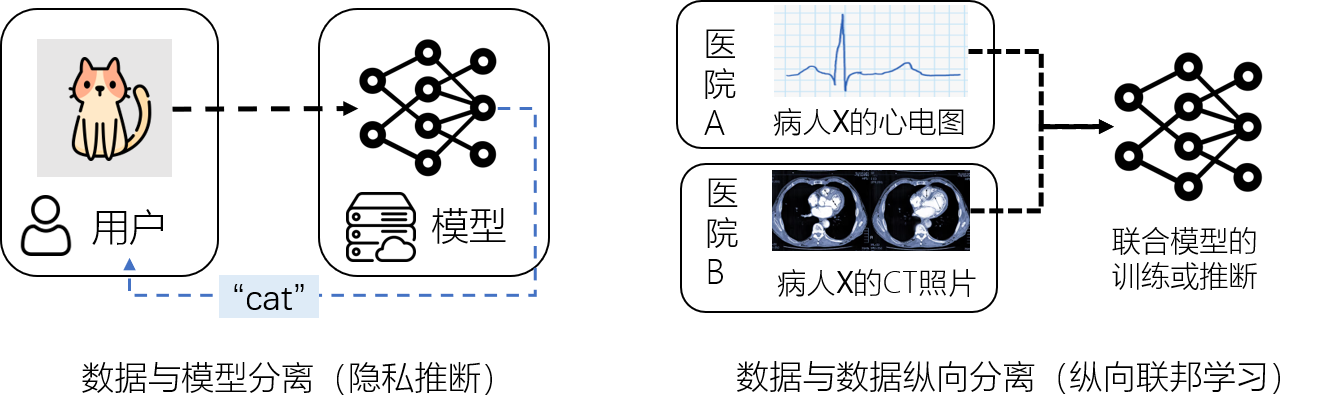
\includegraphics[width=1\linewidth]{Z_Resources/PPML-overview.png}
    \caption{人工智能应用中的三大隐私保护场景}
    \label{fig:intro:ppml-overview}
\end{figure}


人工智能应用中的隐私保护主要可以分为三个场景,分别是数据与模型分离的“隐私推断(Private Inference)”场景~\cite{mann_2023_secure_inference}、数据与数据纵向分离的“纵向联邦学习(Vertical Federated Learning)”场景~\cite{liu2024vertical}、以及数据与数据横向分离的“(横向)联邦学习(Federated Learning)”场景~\cite{yangqiang2019federated}。
%
我们将其呈现在\autoref{fig:intro:ppml-overview}中。
%
其中数据与数据横向分离场景中的数据隐私问题已经有联邦学习这一较为成熟的解决方案~\cite{yangqiang2019federated}。
联邦学习的基础范式为联邦平均(Federated Averaging)算法~\cite{mcmahan_2017_fedavg},其通过多个参与方在本地训练模型然后在服务器上以参数平均等方式聚合,从而保护各个参与方的数据隐私。
%
虽然联邦学习的实现较为简单高效,但是其应用场景局限在数据横向分布(各方拥有具有相同格式的不同样本)的模型训练阶段,且无法保护模型的隐私,因此具有一定的局限性。
%
而本文所讨论的隐私保护机器学习(Privacy-Preserving Machine Learning)是解决人工智能应用中的隐私问题的一种较为通用的解决方案~\cite{al_2019_ppml,xu_2021_ppml}。
%
其通过密码学~\cite{evans_2018_pragmatic_mpc}、拆分学习~\cite{vepakomma2018split}等多种方法,实现对人工智能模型训练或推断过程中的隐私保护,可以适配多种人工智能模型的训练和推断场景。
%
与联邦学习的场景互补,本文中所讨论的隐私保护机器学习方案往往考虑在单次计算中参与方较少的场景,对应数据与模型分离以及数据与数据纵向分离的场景。
%
对于包含大量参与方的联邦学习场景,可以通过各个参与方将数据以加密的形式上传至指定的几个服务器,从而将其转化为隐私保护机器学习问题。

隐私保护机器学习的核心问题在于效率和安全。
%
基于密码学的隐私保护机器学习,能够达到很高的安全性,并且可以对安全性进行严格的数学证明,但是其需要复杂的多方交互计算以及昂贵的密码学加解密运算。
随着人工智能模型的规模日益庞大,许多类似ChatGPT的大规模模型被提出~\cite{chatgpt,touvron_2023_llama,duzhengxiao_2022_glm},其对计算能力的要求逐步提升,导致基于密码学方法的效率往往难以达到实用的标准~\cite{hou2023ciphergpt}。
%
而拆分学习相比密码学方法有着较高的效率,但是其安全性缺少严格的证明,许多研究也提出了针对拆分学习的攻击方法~\cite{hezecheng_2019_model_inversion_attack,abuadbba2020can_split},
同时,当前对于其效率优化的研究也较为缺少。
%
上述的效率和安全问题制约了隐私保护机器学习的应用,因此如何更好地平衡隐私保护机器学习的效率和安全,是当前人工智能隐私领域亟待解决的问题。
%
通过优化隐私保护机器学习的效率和安全,可以使得人工智能的应用更加广泛,并且更好地保护用户的隐私权和人工智能公司的数据及模型资产,推动人工智能产业可持续发展。




    \chapter{相关研究综述}
隐私保护机器学习(Privacy-Preserving Machine Learning)指的是在保护数据以及模型隐私的前提下进行机器学习模型的训练和推断。
%
当前的隐私保护机器学习包含了基于密码学的隐私计算、拆分学习、联邦学习、可信执行环境、差分隐私等多种方法。
%
基于密码学的隐私计算~\cite{al_2019_ppml}通过各种密码学底层技术实现可证明安全的隐私保护机器学习,但是由于牵涉到大量密码学计算,会带来较高的通信和计算开销。
%
拆分学习~\cite{vepakomma2018split}通过切分模型和交换中间结果实现隐私的训练和推断,具有实现简单、计算和通信开销小的优点,但是由于部分模型和中间结果的暴露,存在一定的隐私泄露风险。
%
联邦学习\cite{yangqiang2019federated,mcmahan_2017_fedavg}通过多个参与方聚合模型来保护各个参与方的本地数据隐私,适用于数据横向分割、训练阶段的场景。
%
可信执行环境~\cite{sabt_2015_tee,2016_intel_sgx}将模型和数据装载入特定可以被信任的硬件中进行运算,与外部环境隔离,从而实现隐私保护。
%
差分隐私~\cite{dwork_2006_differential_privacy,wuruihan_2023_label_dp}通过在计算过程中加入特定分布的噪声,使得计算结果满足一定的隐私性,可以控制输入数据的隐私泄露程度,但是其必须在隐私保护程度和计算精确性之间进行权衡~\cite{abadi_2016_dp_dl}。
%
上述的几类方法彼此相对独立,但是又在一定程度上相互重叠,大量研究~\cite{zhangqiao_2018_gelu_net,bonawitz_2017_secure_agg,thapa_2022_splitfed,zhou_2022_codesign,riazi_2018_chameleon,weikang_2020_fed_dp}采用其中的多种方法来共同构建新的隐私保护机器学习方法,旨在更好地平衡效率和隐私。
%
本文主要研究通用的适用于多方场景的隐私保护机器学习的训练和推断算法框架,因此聚焦于拆分学习、密码学方法以及密码学和非密码学的混合方法三个方面。
%
本章节对以上的三个方面的研究现状逐一进行更细致的介绍。

\section{基于拆分学习的隐私保护机器学习}
%
拆分学习~\cite{vepakomma2018split,poirot2019split}是纵向联邦学习(Vertical Federated Learning)~\cite{liu2024vertical}的主流范式,指的是在纵向联邦学习中,把模型拆分成多个部分划分给不同的参与方,参与方之间相互交换中间结果和梯度,从而实现模型的正向传播和反向传播。
%
在此过程中,各方的输入数据并未直接泄露,因此拆分学习被认为在一定程度上可以保护隐私。

\begin{figure}[h]
    \centering
    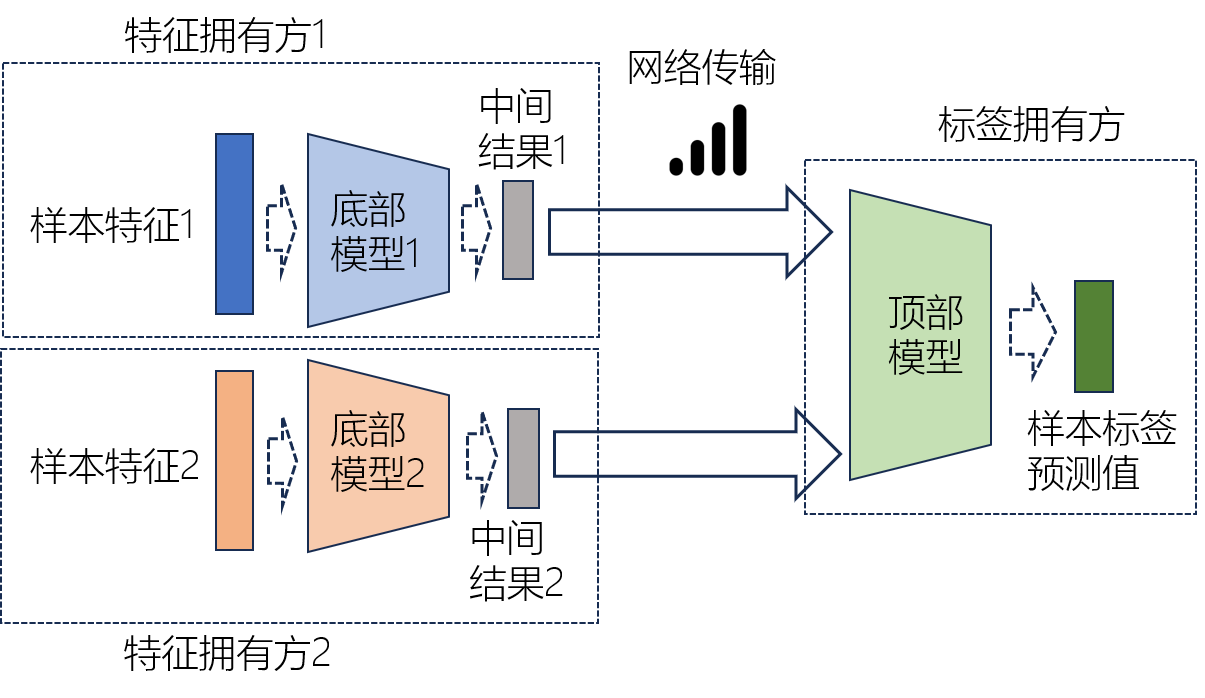
\includegraphics[width=0.8\linewidth]{Z_Resources/拆分学习示意图.png}
    \caption{拆分学习示意图}
    \label{fig:related_work:split_learning}
\end{figure}

一个简单的拆分学习例子如\autoref{fig:related_work:split_learning}所示。
%
此时纵向联邦学习有3个参与方(记作$P_1, P_2, P_3$),分别拥有样本特征第一部分($\bvec x_1$)、样本特征第二部分($\bvec x_2$)和样本标签($\hat y$)。
%
相应地,模型也被划分成了3个部分,分别是底部模型第一部分($M_{b1}$,参数记为$\Theta_{b1}$),底部模型第二部分($M_{b2}$,参数记为$\Theta_{b2}$),以及顶部模型($M_t$,参数记为$\Theta_h$)。
%
在前向传播的过程中,$P_1$和$P_2$分别本地计算得到各自的中间结果:
$
    \left(
        \bvec h_1 = M_{b1}(\bvec x_1;\Theta_1),
        \bvec h_2 = M_{b2}(\bvec x_2;\Theta_2)
    \right)
$,
然后将其发送给$P_3$(标签拥有方)。
%
$P_3$接收到$\bvec h_1, \bvec h_2$之后,将其输入到顶部模型,计算得到模型输出$y = M_t(\bvec h_1, \bvec h_2; \Theta_h)$。
%
这样便完成了一次前向传播过程。
%
%
在反向传播过程中,$P_3$通过模型的预测标签($y$)和真实标签($\hat y$),计算出损失函数$L(y, \hat y)$,并且将其对于顶部模型和中间结果的参数求梯度得到${\partial L(\hat y, y)}/{\partial \Theta_t}, {\partial L(\hat y, y)}/{\partial \bvec h_1}$ 和 ${\partial L(\hat y, y)}/{\partial \bvec h_2}$.
%
其中,前者被标签拥有方用于更新顶部模型参数,而后两者则发给相应的特征拥有方用于计算损失函数相对于底部模型参数的梯度。
%
该计算通过链式求导法则进行,以$P_1$为例:
\begin{equation}
    \dfrac{\partial L(\hat y, y)}{\partial \Theta_{b1}} = \dfrac{\partial L(\hat y, y)}{\partial \bvec h_1}\cdot \dfrac{\partial \bvec h_1}{\partial \Theta_{b1}}.
\end{equation}
%
注意,上式中的${\partial \bvec h_1}/{\partial \Theta_{b1}}$是雅可比矩阵,链式法则中的乘法也是对应的矩阵乘法运算。

拆分学习具有原理简单、实现方便、计算和通信开销小、可以适用于不同的深度学习模型等优势,因此其已经被应用于很多需要考虑数据隐私的领域,如:医疗影像分割\cite{roth2022split_unet}、边缘设备中的图像分类\cite{fagbohungbe2022split_edge_image,palanisamy2021spliteasy}、毫米波接收功率预测\cite{koda2020split_mmwave}等。

\subsection{拆分学习中的隐私问题}
虽然拆分学习具有实现简单、效率高等诸多优势,但是在训练和推断过程中,各方直接交换了中间结果和中间梯度的明文,从而存在一定的隐私泄漏风险。
%
拆分学习的隐私泄露可以分为两类:特征拥有方的隐私泄露和标签拥有方的隐私泄露。
%
下面将对这两种隐私泄露分别进行介绍。
%
\subsubsection{特征拥有方的隐私泄露}
在拆分学习的过程中,特征拥有方将底部模型产生的中间结果,也就是神经网络的隐层表征(Hidden Representation),直接发送给了标签拥有方。
%
作为输入特征经过变换的结果,隐层表征必然包含了输入特征的信息。
%
假设攻击者腐化了标签拥有方,便可以通过各种手段从隐层表征中恢复出部分输入特征的信息。
%https://www.overleaf.com/project/6564295824afdb06585a588e#
因此,近年来也有许多工作研究了拆分学习中特征拥有方的隐私泄露问题,现总结如下:
%
\begin{enumerate}
    \item 在卷积神经网络中,隐层表征直接包含了输入的信息\cite{abuadbba2020can_split}。
    由于卷积层的局域运算特性,其会保留图像本身的大致形状、轮廓等信息。
    即便经过多个卷积层后,隐层表征依然能够保留图像的整体轮廓,从而使得原始图像的数据出现一定程度的泄露。
    %
    \item 攻击者可能训练一个逆向网络从隐层表征中重构出原始输入特征~\cite{vepakomma2020nopeek,hezecheng_2019_model_inversion_attack}。
    一种简单的情况可以是,攻击者能够获取一部分泄漏的样本特征$(\bvec x_1, \cdots, \bvec x_n)$和对应的隐层表征$(\bvec h_1, \cdots, \bvec h_n)$,则最优的重构函数$R_*$可以定义为:
    \begin{equation}
        R_* = \mathop{\text{argmin}}_{R} \sum_{i=1}^n \Vert R(\bvec h_i) - \bvec x_i\Vert^2 = 
        \mathop{\text{argmin}}_{R} \sum_{i=1}^n \Vert R(M_b(\bvec x_i)) - \bvec x_i\Vert^2,
    \end{equation}
    其中,$\Vert \cdot\Vert^2$ 表示二范数平方,也可以按照具体情况换成其他的函数来度量重构效果。
    一般可以采用一个和底部模型相对应的神经网络作为重构函数,比如原始模型是是多层卷积,则$R$可以主要由反卷积(ConvTranspose)构成。
    %
    \item 如果攻击者本身拥有底部模型的参数信息,则可以采用白盒攻击的形式,优化$\bvec x'$使得$M_b(\bvec x')$尽可能接近$\bvec h = M_b(\bvec x)$~\cite{hezecheng_2019_model_inversion_attack,luoxinjian2021feature_attack}:
    \begin{equation}
    \label{eq:related_work:whitebox-reconstruction}
        \bvec x'_* = \mathop{\text{argmin}}_{\bvec x'} \Vert M_b(\bvec x') - \bvec h\Vert^2 = \mathop{\text{argmin}}_{\bvec x'} \Vert M_b(\bvec x') - M_b(\bvec x)\Vert^2.
    \end{equation}
    %
    注意到\autoref{eq:related_work:whitebox-reconstruction}可能有无穷多个解,影响重构效果。为了提高重构效果,也可以在损失函数中加入关于输入特征的先验知识。
    %
    比如输入特征是图像,则可以在损失函数中加入$\bvec x'$的总变差(Total Variance),使得重构出来的结果更接近实际图像;
    如果攻击者有同一样本的额外特征$\bvec z$,则可以将$\bvec x'$替换为$g(\bvec z)$,这里假设想要攻击的输入特征和攻击者获取的额外特征有关。
    %
    \item 在训练过程中,攻击者可以对训练目标进行修改,使得中间结果包含更多关于输入特征的信息。比如假设攻击者拥有一部分泄漏的样本特征$\{ \bvec x' \}$,
    则他可以先训练一个自编码器~\cite{kramer1991autoencoder,baldi2012autoencoders}$(f,f^{-1})$使得$f^{-1}\circ f(\bvec x')\approx \bvec x'$。
    %
    在拆分学习训练过程中,攻击者采用对抗训练的方式,使得待攻击样本的隐层表征$\bvec h = M_b(\bvec x)$与自编码器编码的泄漏样本的特征$f(\bvec x')$尽可能接近。
    %
    于是攻击者可以直接通过$f^{-1}(\bvec h)$来重构原始的输入特征~\cite{pasquini2921inference_attack_tiger}。
    %
\end{enumerate}

值得注意的是,第4种方法需要攻击者改变正常的拆分学习训练过程,而前面介绍的3种方法则不需要改变训练过程。
%
一般将主动改变训练过程的攻击者称为“主动攻击者(Active Attacker)”,反之则称为“被动攻击者(Passive Attacker)”。
%
主动攻击者往往能取得更强大的攻击效果,但是由于其对训练本身的改变,可能导致训练效果变差、训练速度变慢等问题,会更容易被检测出来,且无法在模型推断阶段进行攻击。
与此相反,被动攻击者的攻击效果会更低,但是具有更好的隐蔽性。

\subsubsection{标签拥有方的隐私泄露}
对于标签拥有方的隐私泄露,我们考虑的是攻击者腐化特征拥有方的情况。
%
标签拥有方的隐私泄露主要来源于两个方面:
\begin{enumerate}
    \item 隐层表征(中间结果)导致的标签信息泄露。
    深度学习模型学习的过程,可以看做一个将输入特征逐渐转化成标签的过程。
    因此,随着训练的进行,隐层表征会逐渐变得与标签更为相关。
    %
    许多将神经网络隐层表征可视化的工作也显示出,随着训练的进行,隐层表征逐渐按照对应的标签聚类成不同的簇;且越靠近输出的隐层表征和标签关联度越大~\cite{paulo2017visualize_hidden,pezzotti2017deepeyes,cantareira2020hidden_vector_fields}。
    %
    在这种情况下,攻击者就可以根据隐层表征来推断输入数据的标签。
    %
    即使在没有任何额外信息的情况下,攻击者也可以对隐层表征进行聚类,从而获取输入样本的类别关系~\cite{liujunlin2022clustering_attack,liujunlin2023distance_attack}。
    %
    如果攻击者能够获取少量泄漏的隐层表征和对应的标签,也可以自己训练一个顶部模型,并且获得很好的分类效果~\cite{fucong2022label_infer_attack}。
    %
    \item 隐层表征的梯度导致的标签信息泄露。
    与隐层表征类似,隐层的梯度和标签信息也呈现出非常强的相关性。
    %
    比如在二分类模型中,同类样本的梯度间的余弦相似度接近1,而异类样本的梯度间的余弦相似度则接近-1,直接暴露了样本的类别信息~\cite{oscarli2022label_defense_marvell}。
    %
    此外,也可以通过优化替代样本的梯度,使其尽可能接近攻击者获取到的梯度,从而复原出样本的标签~\cite{erdogan2022unsplit}。
    %
    具体方法如下:
    \begin{equation}
        \mathop{\text{argmin}}_{\Theta_t', \hat y'} \left\Vert \dfrac{\partial L[\hat y', M_t(M_b(\bvec x);\Theta_t')]}{\partial M_b(\bvec x)} - \dfrac{\partial L[\hat y, M_t(M_b(\bvec x);\Theta_t)]}{\partial M_b(\bvec x)} \right\Vert^2,
    \end{equation}
    其中,$\bvec x, \hat y$ 是原样本的特征和标签,而$\hat y'$是随机初始化的替代标签;$\Theta_t, \Theta_t'$分别表示原始的顶部模型参数和替代的顶部模型参数。
    通过优化替代的样本和顶部模型参数,可以恢复出样本的标签。
\end{enumerate}

标签泄露不仅仅带来了样本标签的隐私问题,同时还会泄露模型本身。
%
如上文所述,当特征拥有方腐化(Corrupted)后,它可以利用少量标签(或直接聚类生成标签),训练出顶部模型。
%
由于在模型训练的后期,底部模型的表征提取能力已经很强,固定底部模型后,攻击者很容易就可以训练出一个表现良好的顶部模型,从而得到整个完整的模型。
%
因此,这种攻击也被称为“模型补全攻击(Model Completion Attack)”~\cite{fucong2022label_infer_attack}。
%
在这种情况下,腐化的特征拥有方可以窃取几乎标签拥有方的所有资产(标签和顶部模型),从而使得拆分学习的隐私保护能力受到严重损害。


\subsubsection{总结}
%
无论是输入特征的泄露还是标签的泄露,都与许多因素有关,包括模型结构和拆分的层数。
%
显而易见的是,如果分割点靠近模型输入,则隐层表征泄漏的特征信息更多;而分割点接近模型输出,则会泄露更多关于标签的信息。
%
这也是著名的数据处理不等式(Data Processing Inequality)的推论。
%
模型的结构也对隐私泄漏的程度有很大的影响。
%
从输入特征的角度而言,
%
对于卷积神经网络,卷积层的隐层表征与输入十分相关,且很多网络的隐层维度也很高,因此很容易被攻击者重构出输入特征~\cite{abuadbba2020can_split};
%
对于全连接网络,如果隐层维度小于数据维度,则会存在无穷多组输入拥有同样的隐层表征,
这导致没有先验知识的情况下,攻击者难以获取输入特征信息;
%
基于Transformer结构的语言模型,包括时下流行的大语言模型(Large Language Model),拥有很高的隐层表征维度,并且保留了序列结构,因此攻击者也可以轻易地从隐层表征中重构出原始的输入文本~\cite{morris2023embedding_almost}。
%
从标签的角度而言,更低的隐层表征维度往往意味着更容易恢复出标签,因为高维度的特征中可能包含许多与标签无关的信息,使得攻击者更难从中提取出标签~\cite{oscarli2022label_defense_marvell,sunjiankai2022forward_embedding_protect}。


\subsection{拆分学习的隐私保护方法}
为了解决前文所述的拆分学习中的隐私泄露问题,一些研究也提出了保护拆分学习中输入特征和标签的隐私的方法,当前主要采用的方法是对隐层表征或隐层梯度进行扰动。

首先介绍对隐层表征进行扰动,使其与输入特征或标签特征不相关的方法。
%
由于隐层表征、输入特征、标签的维度可以是任意的,因此常用的皮尔逊相关性(Pearson Correlation)并不适用。
%
因此现有工作主要采用距离相关性来衡量隐层表征和输入特征、标签的相关性~\cite{vepakomma2020nopeek,sunjiankai2022forward_embedding_protect}。
%
距离相关性(Distance Correlation)~\cite{szekely2007dcor,szekely2009brownian_dcor}是一种特殊的相关性度量,可以度量不同维度的随机向量之间的相关性,并且可以度量非线性的相关性,距离相关性为0当且仅当两个变量是无关的(互信息为0)。
%
使用距离相关性来保护输入特征或标签信息的损失函数可以写为:
\begin{equation}
    L' = L_0 + \alpha \text{Dcor}(H, X) + \beta \text{Dcor}(H, Y),
\end{equation}
其中,$\text{Dcor}(\cdot, \cdot)$表示距离相关性,$X,H,Y$分别表示当前批次的输入特征、拆分层表征和标签,$\alpha,\beta$则用于控制扰动程度。
%
注意到,此处的距离相关性计算是通过批样本的经验分布(Empirical Distribution)进行估计的,因此需要较大的批大小(Batch Size),否则估计值会出现较大的误差。
%

针对隐层梯度泄露标签信息的情况,Marvell方法~\cite{oscarli2022label_defense_marvell}通过最小化正样本和负样本之间的隐层梯度间的KL散度来保护样本的标签信息。
%
当标签拥有方计算出隐层梯度$g = \partial L/\partial \bvec h$时,它会对其加入一个正态分布的噪声$D \sim \mathcal N(0, \Sigma_D)$,然后将其发给特征拥有方。
%
具体的优化问题可以写做:
\begin{equation}
\begin{split}
\label{eq:related_work:marvell}
    & \min_{\Sigma_D^+,\Sigma_D^-} \text{KL}\left[\mathcal N(\mu_g^+, \Sigma_g^+ + \Sigma_D^+)\Vert\mathcal N(\mu_g^-, \Sigma_g^- + \Sigma_D^-)\right],
    \\
    & \text{s.t.}\quad p\text{tr}(\Sigma_D^+) + (1-p)\text{tr}(\Sigma_D^-) \le P,
\end{split}
\end{equation}
这里假设正样本和负样本的原始的隐层梯度也分别满足正态分布$\mathcal N(\mu_g^+, \Sigma_g^+)$和$\mathcal N(\mu_g^-, \Sigma_g^-)$,
而$\Sigma_D^+,\Sigma_D^-$则分别是给正样本和负样本的隐层梯度家的噪声的协方差矩阵。
%
约束条件中的$p$和$1-p$分别代表正样本和负样本的频率,$P$表示设定的噪声大小的平均值上限,用于控制噪声的规模,防止添加的噪声太大。
%


上述对隐层表征和梯度的扰动方法均存在一些缺陷。
%
在隐层表征维度高的情况下,距离相关性的估计会变差,从而使得其保护效果大幅度降低~\cite{erdogan2022unsplit}。
%
而Marvell方法~\cite{sunjiankai2022forward_embedding_protect}虽然对梯度进行了扰动,并不能防止从隐层表征直接推出样本标签的情形,
同时该方法也仅适用于二分类场景。
%
因此,如何保护拆分学习过程中的特征和标签隐私,依然是个极具挑战性的问题。


\subsection{拆分学习的效率提升}
相对于基于密码学方法的隐私保护机器学习,拆分学习具有较小的开销,因为拆分学习仅仅是在明文计算的基础上,传输隐层表征和隐层梯度,并未引入额外的计算。
%
但是考虑到许多神经网络的隐层尺寸较大,因此在通信效率方面,拆分学习依然存在可以优化的空间。
%
一种简单的思路是将稀疏(Sparsification)和量化(Quantization)方法引入拆分学习,对隐层表征和隐层梯度进行压缩,从而减少拆分学习训练和推断过程中的通信量。
%

\textbf{稀疏化:}
对一个向量(或矩阵、张量)进行稀疏化,指的是将其(绝对值)较大的元素保留,而将其绝对值较小的元素丢弃,即设置为0。
%
稀疏化有效性基于“较大的元素在计算过程中较为重要,而较小的元素在计算过程中可以忽略”这一假设。
%
稀疏化之后,数据的传输格式也会发生变化。一种简单的做法是将数据以“(下标,值)”的形式进行编码。假设原有的数据位数为$L$(如对于32位浮点数$L=32$),数据的总量为$N$,稀疏率为$p$,则简单的下标-值编码方法可以实现压缩比率(压缩后大小/压缩前大小)为:
\begin{equation}
    \text{压缩比率}=\dfrac{pN(L + \lceil \log_2N \rceil)}{NL} = p(1 + \dfrac{\lceil \log_2N \rceil}{L}).
\end{equation}
为了提高压缩比率,可以采用更加先进的数据压缩方法,如经典的Huffman编码~\cite{huffman1952}可以直接应用于稀疏化后的数据(的二进制表示)上。
%
更为适合稀疏化的编码为对下标的差值(Run-length)序列进行Golomb编码~\cite{gallager1975golomb}。
%
如果在一批数据中,每个下标被稀疏化的概率是均等的,则Golomb编码具有最小的期望压缩比率,大约可以在下标-值编码的基础上再减少一半~\cite{sattler2019sparse_binary}。
%
值得注意的是,采用编码方案虽然减少了通信开销,但是也会带来一定的计算开销。


\textbf{量化:}
量化指的是降低数据的精确度,使用较少的比特位保留数据,在尽可能保证数据的准确性的情况下,压缩其存储空间。
%
一般的机器学习模型的训练或推断采用的都是32位浮点数,通过量化的方式,可以将模型的权重、模型计算的中间结果等压缩到更低位数(如8位,4位,甚至1位),从而减少模型大小或降低模型计算过程中的内存开销和计算开销~\cite{zhou2016dorefa,banner2018_8bit,yang2019quantization}。




利用稀疏化和量化减轻通信量的方法,在分布式计算、横向联邦学习领域被广泛应用~\cite{wen2017terngrad,sattler2019sparse_binary}。
%
此时,稀疏化和量化可以同时被应用在表征和梯度上,从而减少了每轮训练过程中的通信量开销。
%
虽然稀疏化和量化导致梯度不准确,由于使用随机梯度下降(Stochastic Gradient Descent)优化时,批样本梯度本身有一定噪声,甚至被认为对收敛(Convergence)和泛化(Generalization)是有益的~\cite{hardt2016sgd,goyal2017sgd_imagenet,chaudhari2018sgd}。
%
同时,相关研究也表明,稀疏化和量化并未对模型最终的结果有显著影响,而训练到一个较高准确度的通信量也显著小于常规训练的通信量~\cite{aji2017sparse,sattler2019sparse_binary,wen2017terngrad}。

%
但是拆分学习作为一个较新的领域,其通信效率提升的研究相对较少。
%
Castiglia等人~\cite{castiglia2022compressed_vfl}研究了基本的Top-$k$稀疏化、(标量)量化以及向量量化(Vector Quantization)在拆分学习中的应用,并且证明了其收敛性。
%
具体而言,拆分学习训练时的前向传播过程被更改为
\begin{equation}
\label{eq:split-compress}
    Y = M_t(\mathsf{Compress}[M_b(X)]),
\end{equation}
%
其中,$M_t$表示顶部模型,$M_b$表示底部模型,$X, Y$ 表示输入特征和模型预测值,$\mathsf{Compress}$表示压缩操作(如稀疏、量化)。
%
尽管收敛性得到证明,但是该文采用的压缩方法最多只能将压缩率降低到1/16,且常规的稀疏和量化(除了向量量化外)对模型最终的效果有较明显的降低。
%
此外,该方法只适用于训练场景,并未考虑推断场景,并且要求公开的顶部模型让各个参与方执行块坐标下降法(Block Coordinate Descent)对自身的参数进行优化。

也有部分研究采用异步更新的方式提高拆分学习的通信效率,其方法包括底部模型多轮本地更新~\cite{fu2022cache_vfl}或是顶部模型多轮本地更新~\cite{chen2021async_split}。
%
这些方法同样针对的是拆分学习训练的场景,并不能应用于推断阶段。
%
此外,Ayad等人~\cite{ayad202vfl}提出使用自编码器压缩中间表征,也就是将\eqref{eq:split-compress}中的$\mathsf{Compress}$替换为一个自编码器,从而实现训练和推断过程中的通信优化。
%
但是该方法需要针对特定模型定制自编码器,并非一种通用的方法。
\section{基于密码学的隐私保护机器学习}
纵向联邦学习可以看作是特定的一类隐私计算问题,即:在保护数据和模型参数的情况下进行模型的训练和推断,因此也可以通过基于密码学的安全多方计算(Secure Multiparty Computation)来实现。
%
\begin{definition}[安全多方计算]
    有$n$个参与方$P_1, \cdots, P_n$与各自的输入$X_1, \cdots, X_n$,以及一个公共函数$f$,安全多方计算指的是各方根据指定的协议交互计算出$Y= f(X_1, \cdots, X_n)$($Y$可以是公开的或是被指定的参与方获得,两种定义是等价的),同时保护各方输入的隐私。
\end{definition}
%
注意安全多方计算的定义隐含了安全性设定(Security Setting),也就是对于各个参与方行为的限制条件,包括:各个参与方忠实执行计算协议但是同时利用自己获取到的一切信息,称为半可信(Semi-honest)安全性设定,以及参与方可能存在不遵守计算协议的情况,称为恶意(Malicious)安全性设定,以及在上述两种情况下部分参与方共谋(Collusion)的情况。
%
复杂的安全性设定可能导致极为复杂的协议设计和安全性证明。
%
本文遵循一般隐私保护机器学习中的半可信安全性设定。
%
%


安全多方计算协议往往基于几种特定的密码学原语来实现,包括秘密分享(Secret Sharing)、同态加密(Homomorphic Encryption)、混淆电路(Garbled Circuits)等。
%
下面对此进行简要介绍。
%


\textbf{秘密分享}:
秘密分享~\cite{shamir1979share}指的是把一个值分享给多个参与方,其中一定数量的参与方合作才能恢复出该值。
%
具体而言,
%
$(t,n)$-秘密分享指的是将一个值$x$分享给$n$方$P_0, \cdots, P_{n-1}$,其中$P_i$得到的值记作$\langle x \rangle_i$。
%
至少要$t$个参与方一起,才能恢复出$x$的值。低于$t$个参与方则无法得到任何关于$x$的信息。
%
常用的秘密分享包括两方加法分享(Additive Sharing)以及两方布尔分享(Boolean Sharing),这两种分享分别把一个数$x$拆分成两个随机数相加($x = \langle x \rangle_0 + \langle x \rangle_1$)或是两个随机数(按位)异或($x = \langle x \rangle_0 \oplus \langle x \rangle_1$)。
%
在秘密分享的情况下,进行加法(异或)只需各方本地运算,但是进行乘法(异与)较为复杂,一般可以采用离线(Offline)计算的Beaver三元组进行~\cite{beaver1992efficient},即:在获得具体的输入前,两方通过一定方法计算出一组秘密分享的随机数$(u,v,w)$满足$uv = w$。
%
一般可以使用同态加密、不经意传输(Oblivious Transfer)等手段,在三方场景下,可以使用一个半可信第三方分发从而提高离线计算的效率。
%
注意秘密分享一般在有限域上进行,如:加法分享在模$N$的整数环$\mathbb Z_N$进行,布尔分享按照定义在$\mathbb Z_2$进行)。
%
此时各方所获取到的值都是在有限域上均匀分布的随机数,与实际值无关,因此实现信息论安全(Information-Theoretic Security)。


\textbf{同态加密}:
同态加密是一类特殊的加密算法,其支持在密文上进行一定的计算,使得解密的结果和明文计算一致。
%
令某种加密系统的加密函数为\textsf{Enc},解密函数为\textsf{Dec}。
%
如果对于某个定义在明文上的运算符$\mathsf{OP}_P$,存在密文上的运算符$\mathsf{OP}_C$,使得对于任意明文$X, Y$都满足:
\begin{equation}
    \textsf{OP}_P(X, Y) = \mathsf{Dec}[\mathsf{OP}_C (\mathsf{Enc}[X], \mathsf{Enc}[Y])],
\end{equation}
%
则称该加密系统可以同态地计算$\mathsf{OP}_P$的运算。
%
注意$\mathsf{OP}_P$ 往往不等于 $\mathsf{OP}_C$。
比如,Paillier同态加密支持明文加法,即:$\mathsf{OP}_P=$`$+$',但是对应的密文运算是乘法,也就是$\mathsf{OP}_C=$`$\times$'。
%
同态加密按照支持的运算的不同,一般可以分为半同态加密(Partial Homomorphic Encryption)和全同态加密(Fully Homomorphic Encryption)。
%
半同态加密支持一种同态运算,如加法或乘法,分别可以称为加同态加密和乘同态加密。
%
全同态加密同时支持加法或乘法。
%
除此之外,还有分级(Leved)全同态加密,其只支持一定次数多乘法运算。
%
当前常用的同态加密包括Paillier加同态加密~\cite{paillier1999},其定义域为大整数;BFV/BGV全同态加密~\cite{2012bfv1,2012bfv2,2014bgv},其定义域为整系数多项式;以及CKKS全同态加密~\cite{ckks2017},其定义域是实系数多项式,并且运算过程会产生一定的误差。


\textbf{混淆电路}:
混淆电路由姚期智院士于1986年提出~\cite{yao1986gc},是一个两方安全计算协议,可以用于计算任意布尔电路。
%
混淆电路通过对原始电路的逻辑门进行“混淆”得到,具体而言,每个门的输入和输出都变成了随机数,因此无法根据混淆后的电路的输入、输出以及中间值,获取关于原始电路输入输出值的任何信息。
%
混淆电路的执行过程可以表示为:给定一个公开函数$f$,某方(这里设为$P_0$)产生一个布尔电路$C$,然后对其进行混淆得到混淆电路$C^G$,并发送给另一方(这里设为$P_1$);同时,$P_0$自身的输入$X_0$ 混淆后得到 $X_0^G$
%
同时,$P_1$和$P_0$ 执行不经意传输协议,获取$P_1$输入的混淆值 $X_1^G$。
%
然后$P_1$可以根据混淆输入计算出混淆输出:$Y_G = C_G(X_0^G, X_1^G)$,将其返还给$P_0$后,$P_0$根据自身维护的混淆表得到实际的输出值。
%
混淆电路只需要常数轮的通信即可计算任何门电路的值,但是因为电路中的每个布尔值都转化成了高位的随机数,会消耗大量通讯流量;由于涉及密码学计算,也有较大的计算开销。
%
混淆电路发展至今有多种优化方案提出,包括Free-XOR~\cite{kolesnikov2008free_xor},HalfGate~\cite{zahur2015halfgate}等,降低了通讯和计算开销。
%

除去以上介绍的几种密码学技术,多方安全计算还可以包含其他技术,以及一些定制化的计算协议。
%
下文将对部分主要的基于密码学的隐私保护机器学习研究进行介绍。


\subsection{基于单一密码学技术的隐私保护机器学习}
本节对采用单一密码学技术来实现隐私保护机器学习的相关工作进行介绍。
%
这些工作基于两方的隐私保护机器学习场景,如MLaaS(Machine Learning as a Service),即:用户提供数据,服务方提供机器学习模型。
%

\textbf{基于同态加密}:
2016年微软提出CryptoNets~\cite{gilad2016cryptonets},率先通过同态加密实现神经网络的推断。
%
由于神经网络的权重和输入都被加密,因此这种方法可以实现安全的神经网络推断。
%
CryptoNets采用了YASHE加密算法~\cite{bos2013yashe},这是一种分级同态加密算法,可以支持一定次数的乘法运算、
%
由于同态加密仅仅支持加法和乘法运算,因此CryptoNets将神经网络中的非线性激活函数替换成了平方函数,然后再明文上训练得到模型权重。
%
该方法需要花费数分钟和300Mb左右的流量对MNIST数据集中的一张图片进行分类。
%
%
一些未正式发表的工作~\cite{hesamifard2017cryptodl,chabanne2017pp_dnn}对CryptoNets进行了改进,包括使用更加精确的多项式拟合激活函数、将同态加密算法换为BGV或CKKS等更高效的算法,以及优化同态加密的密文打包技术等。
%
Zhou等人通过将卷积神经网络的权重二值化,实现了更高效的基于全同态加密的神经网络推理~\cite{zhoujunwei2020binary_encrypted_nn}。

\textbf{基于混淆电路}:
DeepSecure框架~\cite{rouhani2018deepsecure}将神经网络模型转化为布尔电路,从而实现隐私神经网络推断。
%
为了提高效率,该框架减少了各类电路中的非异或门数目,从而适配Free-XOR算法。
%
该框架运算速度高于CryptoNets,但是带来了更高的通讯开销。
%
实验表明,一个简单的全连接网络的推断消耗800MB左右的流量。
%
XONN框架~\cite{riazi2019xonn}将二值神经网络(Binary Neural Network)与混淆电路结合,将内积运算转变为异或运算,从而极大地提高了安全推断的效率。


\subsection{基于混合技术的隐私保护机器学习}
为了提高隐私保护机器学习的效率,现有的隐私保护机器学习框架大多将多种密码学技术混合,为机器学习中不同的算子找到最佳的密码学技术。
%

\textbf{两方框架}:
ABY框架~\cite{demmler2015aby}提出将算数秘密分享、布尔秘密分享以及YAO分享(基于混淆电路~\cite{yao1986gc}的两方分享,一方持有混淆值和真实值的对照表,另一方持有混淆电路和混淆值)融合,并且涉及协议对三种分享状态的值进行相互转化,从而为特定的计算任务找到最适合的混合计算协议。
%
SecureML框架~\cite{mohassel2017secureml}将算数秘密分享和混淆电路结合,实现了逻辑回归的推断和训练。
%
其还使用分级同态加密和不经意传输对算数秘密分享的Beaver三元组~\cite{beaver1992efficient}的离线生成进行了优化,并且将Sigmoid函数表示为分段线性函数,通过混淆电路(计算当前值落在哪一段)和算数秘密分享融合来提高计算效率。
%
MiniONN框架~\cite{liujian2017minionn}将秘密分享和混淆电路进一步应用于神经网络推断中,并且使用分段的Spline插值来拟合激活函数,以及采用SIMD(Single Instruction Multiple Data)技术加速了Beaver三元组的生成,从而提高了隐私神经网络的模型准确率和效率。
%
Gazelle框架~\cite{juvekar2018gazelle}使用优化的基于格密码的同态加密(BFV加密~\cite{2012bfv1,2012bfv2})直接加速安全矩阵乘法计算,而非用于产生三元组,从而极大提高了通讯效率;同时采用混淆电路来计算ReLU、最大池化(Max Pooling)等非线性运算。
实验结果表明Gazelle的性能甚至大幅度优于需要依赖第三方的Chameleon框架。
%
Delphi框架~\cite{mishra2020delphi}基于Gazelle框架进行了改进,将同态加密的安全乘法计算用于离线计算Beaver三元组,并利用了神经网络推断过程中权重不变的特性减少了在线的开销;同时将ReLU激活函数替换成二次函数以降低开销。
%
CryptFlow2框架~\cite{rathee2020cryptflow2}基于秘密分享,采用同态加密和不经意传输实现安全乘法,并且新设计了高效的基于不经意传输的安全比较和除法协议,将两方的隐私保护机器学习推广到ResNet等大型模型中。
%
Cheetah框架~\cite{huang2022cheetah}进一步对基于同态加密的神经网络线性运算以及基于不经意传输的ReLU激活函数等非线性运算进行优化。
%si
SIRNN框架~\cite{rathee2021sirnn}通过查真值表的方式计算指数函数,进一步对神经网络中Softmax等非线性函数进行了优化。

\textbf{三方框架}:
Chameleon框架~\cite{riazi_2018_chameleon}混合秘密分享、GMW协议和混淆电路协议进行神经网络计算,在离线阶段使用了可信硬件作为第三方,并采用相关随机性(Correlated Randomness)在各方生成相同的随机数,提高了Beaver三元组产生的效率。
%
ABY3框架~\cite{mohassel2018aby3}基于ABY框架~\cite{demmler2015aby},将秘密分享、布尔分享和混淆电路推广到三方计算的场景以提高效率,并对乘法截断进行了改进。
%
SecureNN框架~\cite{wagh2019securenn}采用了两方秘密分享并且使用第三方来产生Beaver三元组,同时基于比较的布尔运算电路设计了高效的三方安全比较协议,实现了高效的隐私神经网络推断。
%
CryptFlow~\cite{kumar2020cryptflow}是一个支持两方和三方协议的开源框架,其两方协议采用的是ABY协议,而三方协议基于SecureNN框架,对其卷积操作的Beaver三元组进行了优化,同时使用相关随机性来进一步降低通信量;该框架还提供了基于可信执行环境(Trusted Execution Environment, TEE)的恶意安全转换机制,可以将半可信安全的协议转换为恶意安全的协议。
%
Crypten框架~\cite{knott2021crypten}基于秘密分享和GMW协议实现安全的深度学习,并且提供了类似Pytorch风格的接口,使得非密码学专业研究者也可以进行隐私保护机器学习。
%
Falcon框架~\cite{wagh2021falcon}基于ABY3和SecureNN进行了改进,优化了比较协议。
%
AriaNN框架~\cite{ryffel2021ariann}提出使用函数秘密分享(Function Secret Sharing)来计算比较函数,将其降低到仅需一轮通信轮次。

\subsection{其他相关研究}
除了设计安全多方计算框架之外,也有一些其他关于提高基于密码学的隐私保护机器学习效率的研究。
%
比如,
Dalskov等~\cite{dalskov2020secure_q8}研究了将量化(Quantization)技术应用于隐私保护机器学习,将神经网络量化到8比特,并在多个现有的隐私保护机器学习框架上进行了测试。
%
此外,也有许多对于非神经网络的专用机器学习模型进行隐私保护的研究,如树模型~\cite{wu2020vf_tree,fang2021secure_xgb,lu2023squirrel}、聚类模型~\cite{bunn2007secure_kmeans,wu2020secure_kmeans}、矩阵分解~\cite{nikolaenko2013ppmf,kim2018ppmf}等。
%
这些方法往往基于已有的同态加密、混淆电路、多方安全计算协议等技术,对于特定的机器学习模型进行设计和优化。
%


2023年起,随着ChatGPT的出现,大语言模型在工业界和学术界产生了巨大的影响。
%
而大模型的参数量和计算量都极为巨大,即使是明文推断的情况下也对硬件有较高要求,因此对基于密码学的隐私保护机器学习提出了新的挑战。
%
Iron Transformer~\cite{hao2022iron},MPCFormer~\cite{li2022mpcformer},SecureTLM~\cite{chen2024securetlm},PrivFormer~\cite{akimoto2023privformer}等框架在之前研究的基础上,采用同态加密、秘密分享、多项式拟合ReLU、使用特定结构的模型等方法,实现了Transformer模型的隐私保护推断。
%
针对参数量高达数十亿的大语言模型,最近也有研究基于已有的ABY3协议或Cheetah框架进行~\cite{dong2023puma,lu2023bumblebee,hou2023ciphergpt}。
目前这些方案在生成单个输出单词时需要至少进行数十GB的流量传输,在理想环境下也需要数分钟的计算时间,因此依然难以用于实际应用。




\section{密码学与非密码学混合的隐私保护机器学习}
考虑到基于密码学的隐私保护机器学习框架往往开销巨大且实现困难,也有许多研究尝试将密码学和非密码学方法进行融合,从而实现更高效的隐私保护机器学习。
%

一种方法是将同态加密和其他方法结合,将线性计算部分用同态加密实现,而非线性激活函数部分则用明文实现,其计算流程大致可以表示为
\begin{equation}
    \llbracket \bvec y \rrbracket = W \otimes \llbracket \bvec x \rrbracket  + \llbracket \bvec b \rrbracket, \quad \bvec x' = f(\bvec y),
\end{equation}
其中,$\llbracket \cdot \rrbracket$表示加同态加密的密文,$\otimes$ 表示明文和密文的同态乘法,其结果为乘积的密文,$f$表示激活函数,$\bvec x, \bvec x'$分别表示当前层和下一层的输入。
%
GELU-Net算法~\cite{zhangqiao_2018_gelu_net}利用同态加密实现了两方的安全神经网络推断。
该算法假设用户拥有同态加密的私钥。
对于神经网络的每一层,用户将数据上传至服务器,服务器执行同态乘法运算,得到加密的结果后返回给用户,用户再计算非线性的激活函数值。
%
该方法虽然保护了用户的隐私,但是若用户多次进行查询,即可通过对多个输入$\bvec x_i$和输出$\bvec y_i$ 解线性方程组$(W\bvec x_i + b = y_i)$,恢复出神经网络的权重。
%
BAYHENN算法~\cite{xiepeichen_2019_bayhenn}类似GELU-Net,区别在于其采用贝叶斯神经网络来保证模型的隐私。
在贝叶斯神经网络中,模型的权重是随机变量,使得根据输入和输出学习权重转换成一个“噪声学习(Learning With Errors)”问题~\cite{regev_2010_lwe},而该问题被证明是一个困难问题。
%
然而后续研究~\cite{wong_2020_lwe_model}指出,BAYHENN和GELU-Net的安全性都存在问题,很容易被攻击者通过选取特定输入的方式窃取模型参数

此外,还有一些研究通过结合拆分学习和密码学方法,提高了隐私保护机器学习的效率。
Zhou等~\cite{zhou_2022_codesign}提出在多方的纵向联邦学习中使用秘密分享计算神经网络的第一个全连接层,此后在服务器上明文计算。
Chen等~\cite{chen2020vertically}将该方法进一步扩展到图神经网络~\cite{defferrard_2016_gcn,hamilton_2017_graphsage,wuzonghan_2020_gnn_survey}中。
%
BlindFL框架~\cite{fu2022blindfl}将纵向联邦学习的底部模型拆分层使用密码学方法计算,同时明文计算底部模型的其他层和顶部模型。
%
这些方法在一定程度上权衡了效率和隐私,相比于传统的拆分学习,其一般只暴露多个底部模型产生的联合表征而非单一参与方底部模型的输出。
%
但是由于中间结果的暴露,其依然面临着较大的隐私泄漏风险,存在着被逆向攻击的可能性~\cite{hezecheng_2019_model_inversion_attack,abuadbba2020can_split,luoxinjian2021feature_attack,erdogan2022unsplit,qiupengyu_2023_label_selling_you_out}。

综上所述,当前密码学和非密码学方法混合实现隐私保护机器学习的研究仍然处于起步阶段,面临着安全性方面的许多挑战。
%

    
    \chapter{研究方案}
    \section{研究目标、内容和拟解决的关键问题}
    当前隐私保护机器学习的关键问题是隐私和效率问题。
综合已有研究,我们可以对当前的隐私保护机器学习领域总结出如下几条挑战:
\begin{itemize}
    \item \textbf{拆分学习的隐私和效率的进一步优化}:
    拆分学习是纵向联邦学习的一种范式,其通过将模型切分划分给各个参与方的形式来实现一定程度的隐私保护。
    %
    在拆分学习模型的推断和训练中,中间结果需要频繁交换,因此也带来了隐私和效率的问题。
    隐私方面,已有许多研究调查了拆分学习中间结果泄露输入特征和标签信息的问题,但是对应的防护措施却鲜有提出。
    效率方面,不同于联邦学习中通讯压缩的广泛使用,对于拆分学习的效率研究依然处于起步阶段。
    %
    因此,如何对拆分学习的隐私和效率进行优化,是拆分学习走向更广泛应用的一大挑战。

    \item \textbf{更好地混合密码学和非密码学方法来实现效率与隐私的平衡}:
    虽然基于密码学算法的隐私保护机器学习系统有着可证明的安全性,但是其带来的巨大的计算和通讯量使其在许多人工智能模型上难以实用。
    %
    当前的将密码学方法和拆分学习等非密码学方法的研究往往对安全性做出了较大的妥协,有一些研究甚至对其安全性提出了严重的质疑。
    %
    因此,探究如何更好地将密码学方法和非密码学方法结合,同时尽可能保证其安全性影响最小,是让隐私保护机器学习系统走向实用的一大挑战。

    \item \textbf{将隐私保护机器学习应用到更大规模的模型中}:
    随着人工智能和深度学习的发展,模型的规模日益加大,尤其是ChatGPT等大语言模型的兴起,许多模型的参数量已经增长到数十亿甚至百亿、千亿量级。
    %
    在如此大规模的模型上采用密码学方法会带来巨大的计算和通讯开销,难以达到实用水平;而由于大规模模型的中间结果也十分庞大,导致基于拆分学习的方法的隐私泄露大大增加。
    %
    因此,大规模模型的出现和流行给隐私保护机器学习带来了新的挑战。
    %
\end{itemize}


本文针对上述的三大挑战,围绕着拆分学习以及密码学和其他方法混合的隐私保护机器系统进行研究,提出了一系列创新的解决方案,对隐私保护机器学习的效率和隐私进行了更好的优化和平衡,并且提出了在大语言模型上可以实用的、高安全性的隐私保护机器学习系统。
%
本文的研究内容具体如下:
%
\begin{enumerate}
    \item \textbf{基于随机top-$k$算法的拆分学习的通讯效率优化}:
    拆分学习要求每一轮训练或推断都传输拆分层的隐层表征,因此也具有一定的通讯开销,
    %
    在联邦学习中,稀疏和量化等通讯压缩方法已经被广泛使用,但是其在拆分学习中的应用依然鲜有研究。
    %
    本文考虑标签数量大且标签信息不敏感的拆分学习场景,对缩小拆分层维度、top-$k$稀疏化、拆分层L1正则化、拆分层量化等集中基础的通讯压缩方法
    进行了研究。
    %
    通过对收敛性和泛化性的理论分析,最终提出了随机top-$k$稀疏化,在保证模型准确率的基础上大幅降低了拆分学习的通讯和部署开销。
    
    \item \textbf{基于势能损失的拆分学习隐私保护}:
    拆分学习过程中暴露的中间结果带来的隐私泄露问题已经被大量研究提出,如何对此进行防护是一个亟待解决的问题。
    %
    我们针对拆分学习的拆分层表征于模型预测值相关性高的问题,以及随之而来的模型补全攻击进行理论分析,将攻击问题转化为一个有监督或无监督的机器学习问题。
    %
    通过对泛化误差和聚类误差进行分析,并受到静电平衡的物理现象启发,我们提出了基于势能损失的拆分层扰动方法,对拆分层的标签信息提供了有力防护。
    %
    \item \textbf{基于秘密分享和随机排列的隐私保护神经网络}:
    基于密码学的隐私保护机器学习框架的开销主要集中在非线性激活函数的计算上,而对于矩阵乘法之类的线性运算则有较成熟的解决方案。
    %
    而现有的基于密码学和其他方法的混合框架,往往需要暴露中间层结果,在安全性上面临较大的质疑。
    %
    为此,本文利用神经网络中非线性函数的逐元素(Element-Wise)性质,基于半可信的辅助第三方,提出了基于随机排列的算法来计算非线性函数,并与秘密分享的线性计算融合,实现了高效的三方隐私保护神经网络。
    %
    本文还对随机排列的安全性进行了细致的理论和实验分析,表明随机排列带来的隐私泄露小到忽略不计。
 
    \item \textbf{高效的大语言模型安全推理}:
    大语言模型即使是明文也需要极高的计算资源,因此目前的基于密码学的隐私保护机器学习系统应用在大模型上往往会产生更为巨大的通讯和计算开销。
    %
    本文基于此前研究的基于秘密分享和随机排列的隐私保护神经网络框架,结合同态加密技术,针对大模型推理进行了进一步优化。
    %
    考虑到推理过程的权重是不变的,本文将秘密分享的乘法计算过程分为三个阶段,并且减少了重复的秘密分享环节。
    同时,采用了安全的排列协议来计算随机排列,将第三方的所有工作转移到离线阶段进行,进一步提高在线阶段的效率。
    %
    本文提出的大模型隐私推断框架,实现了在常规网络环境下的数秒内两方大模型在线推理,相比于已有算法产生了数百倍的提升。
    %
\end{enumerate}
    \section{研究方法、技术路线、及可行性分析}
    \subsection{研究方法和技术路线}
    针对上节的研究内容,本文提出以下研究方案和路线:
\begin{itemize}
    \item 对拆分学习的效率问题进行调研,重点研究对中间结果进行压缩的方案,并通过实验分析和理论分析考察各种压缩方法的优劣性,提出进一步改进思路。
    \item 对拆分学习的隐私问题进行调研,研究关于模型补全攻击的攻击和防御方法,同时调研神经网络泛化误差和数据分布的相关研究,并进行相关实验模拟。
    \item 对隐私保护机器学习系统进行调研,考察知名密码学协议和开源框架,并着手实现基于秘密分享的隐私计算框架。研究随机排列的安全性,调研距离相关性指标,并通过数值模拟对距离相关性指标进行量化分析。
    \item 对大模型的结构进行研究,考察大模型开源代码,同时考察基于密码学的大模型隐私推断解决方案。考察安全排列协议、隐匿查询协议,对秘密分享协议进行更深入研究,并且着手实现大模型隐私推断框架。
\end{itemize}
    \subsection{可行性分析}
    本课题立足于本人对于隐私保护机器学习和拆分学习的预研成果,具备较强的可行性,具体如下:
\begin{itemize}
    \item 技术可行性:拆分学习和隐私保护机器学习在业界已经被广泛研究,并且在大量机器学习具体应用中证明了可行性。本文对其进行改进和优化,在技术上也是可行的。
    \item 研究积累可行性:本人对拆分学习和隐私保护机器学习已有数篇论文接收或提交投稿,具有足够的积累开展本课题的研究。
    \item 研究条件可行性:本人所在实验室具有充足的实验设备,包括数台装载有NVIDIA 3090/4090 GPU、数十CPU核心的高性能服务器,能够支撑所需用到的深度学习以及密码学相关实验。
\end{itemize}

综上所述,本人对本课题进行了广泛调研,并且有足够的技术积累和硬件条件,可以完成本课题研究。
    \section{研究的创新点}
    本文对应的研究有如下创新点:
\begin{enumerate}
    \item 提出随机top-$k$稀疏化优化了拆分学习的通讯压缩:
    \item 提出势能损失提高了拆分学习的隐私水平:
    \item 将随机排列与秘密分享结合:
    \item 基于随机排列和密码学技术,对大语言模型实现了秒级安全推断:
\end{enumerate}
    \section{研究计划}
    研究计划持续12个月。
\begin{enumerate}
    \item 第1 - 3月:文献调研,考察拆分学习、隐私保护机器学习相关工作。
    \item 第4 - 6月:开始进行方法研究论证,通过理论分析和实现分析手段,对研究方案进行实验调优。
    \item 第7 - 9月:实验和理论的进一步改进,并同步进行相关的投稿工作。
    \item 第10 - 12月:将研究内容进行整合,进行大论文的写作。
\end{enumerate}

    \section{研究基础}
    本人长期研究隐私保护机器学习领域,以第一作者身份发表相关CCF A类论文2篇,SCI论文1篇,以学生一作身份发表SCI论文1篇,以学生二作身份发表CCF B类论文一篇。另有一篇相关专利授权。
此外,有2篇论文已投稿CCF A类期刊/会议,并提交了数项相关专利申请。
}
{
    % 正式论文
    \chapter{绪论}
本章将介绍隐私保护机器学习相关的研究背景、研究现状,梳理本文的研究目的和研究问题,最后总结本文的主要工作和贡献,并呈现本文的组织结构。
\section{研究背景和意义}
近年来,以深度神经网络(Deep Neural Network)为代表的人工智能(Artificial Intelligence)技术在多个领域被广泛应用,包括金融领域的智能推荐、风险控制;媒体领域的智能翻译、语音识别和生成;工业或医学领域的图识别;机器人和自动驾驶领域的智能控制;以及近年来新出现的内容生成领域的文本、图像和视频的生成~\cite{lecun2015deep_learning,zhang2021ai_survey,wang2023chatgpt_survey}。
%
人工智能技术作为近年来广泛发展的新兴技术,在各个领域显示出了其潜力,因此各国企业和政府都在不断加大对人工智能的投入。
%
我国国务院于2017年发布《新一代人工智能发展规划》~\cite{china2017ai_plan},提出“人工智能是引领未来的战略性技术”。
%
美国于2016年提出《国家人工智能研发计划》,并于2019年、2023年进行了两次更新,强调联邦政府必须继续支持人工智能的长期研究~\cite{usa2023ai_plan}。
%
根据2023年世界人工智能大会,目前我国人工智能产业规模以及达到5000亿人民币,企业数量超过4300多家~\cite{2023china_ai_conf}。
%
据Statista数据库的估计,全球人工智能的产业规模在2023年达到1400亿美元,并且将在2030年前后增长到8000亿美元~。

%
数据是人工智能应用的关键一环。
%
训练人工智能模型,往往需要采集大量的数据。
而使用人工智能模型,也需要提供数据才能产生模型的输出。
%
因此,随着人工智能的广泛应用,数据隐私和安全的问题也越来越突出。
%
从用户角度而言,数据被搜集用于人工智能模型的应用将会暴露用户自身的隐私。
%
比如,电商平台的APP为了训练和使用其推荐系统模型,必须采集用户的浏览、点击等行为信息,甚至用户的地址、生活习惯等敏感信息;
使用类似ChatGPT的聊天机器人时,用户的数据也会被发送到模型所在的服务器中。
%
从公司角度而言,如果多个公司想要互相利用对方的数据用于训练更强大的模型,使用一般的人工智能模型的训练方法将数据集中在某个服务器上进行集中式训练,则有数据泄露的风险。
因此,各个公司难以将数据进行共享以训练更强大的模型,形成了“数据孤岛”问题。
%
近年来各国政府也相继出台了有关保护数据隐私的相关法律法规,旨在加强数据的安全使用,防止出现数据滥用和泄露问题。
%
例如:
2021年,我国通过了《个人信息保护法》~\cite{china_personal_information_protection},规定信息处理者有“采取相应的加密、去标识化等安全技术措施”的义务。
2016年欧盟提出的《一般资料保护规则(GDPR)》法案~\cite{GDPR}也要求,数据处理时需要考虑使用匿名化、加密等技术保证数据的隐私。


\begin{figure}[h]
    \centering
    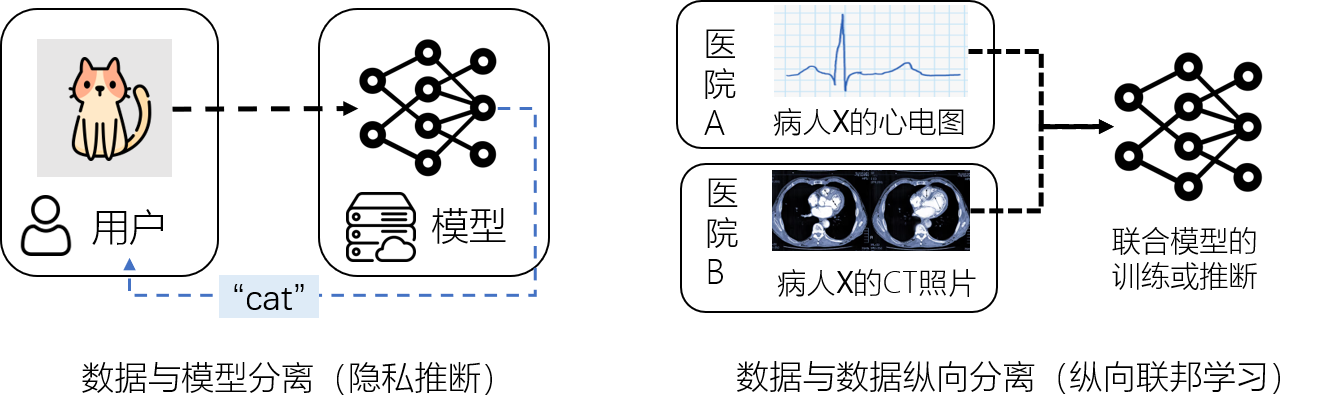
\includegraphics[width=1\linewidth]{Z_Resources/PPML-overview.png}
    \caption{人工智能应用中的三大隐私保护场景}
    \label{fig:intro:ppml-overview}
\end{figure}


人工智能应用中的隐私保护主要可以分为三个场景,分别是数据与模型分离的“隐私推断(Private Inference)”场景~\cite{mann_2023_secure_inference}、数据与数据纵向分离的“纵向联邦学习(Vertical Federated Learning)”场景~\cite{liu2024vertical}、以及数据与数据横向分离的“(横向)联邦学习(Federated Learning)”场景~\cite{yangqiang2019federated}。
%
我们将其呈现在\autoref{fig:intro:ppml-overview}中。
%
其中数据与数据横向分离场景中的数据隐私问题已经有联邦学习这一较为成熟的解决方案~\cite{yangqiang2019federated}。
联邦学习的基础范式为联邦平均(Federated Averaging)算法~\cite{mcmahan_2017_fedavg},其通过多个参与方在本地训练模型然后在服务器上以参数平均等方式聚合,从而保护各个参与方的数据隐私。
%
虽然联邦学习的实现较为简单高效,但是其应用场景局限在数据横向分布(各方拥有具有相同格式的不同样本)的模型训练阶段,且无法保护模型的隐私,因此具有一定的局限性。
%
而本文所讨论的隐私保护机器学习(Privacy-Preserving Machine Learning)是解决人工智能应用中的隐私问题的一种较为通用的解决方案~\cite{al_2019_ppml,xu_2021_ppml}。
%
其通过密码学~\cite{evans_2018_pragmatic_mpc}、拆分学习~\cite{vepakomma2018split}等多种方法,实现对人工智能模型训练或推断过程中的隐私保护,可以适配多种人工智能模型的训练和推断场景。
%
与联邦学习的场景互补,本文中所讨论的隐私保护机器学习方案往往考虑在单次计算中参与方较少的场景,对应数据与模型分离以及数据与数据纵向分离的场景。
%
对于包含大量参与方的联邦学习场景,可以通过各个参与方将数据以加密的形式上传至指定的几个服务器,从而将其转化为隐私保护机器学习问题。

隐私保护机器学习的核心问题在于效率和安全。
%
基于密码学的隐私保护机器学习,能够达到很高的安全性,并且可以对安全性进行严格的数学证明,但是其需要复杂的多方交互计算以及昂贵的密码学加解密运算。
随着人工智能模型的规模日益庞大,许多类似ChatGPT的大规模模型被提出~\cite{chatgpt,touvron_2023_llama,duzhengxiao_2022_glm},其对计算能力的要求逐步提升,导致基于密码学方法的效率往往难以达到实用的标准~\cite{hou2023ciphergpt}。
%
而拆分学习相比密码学方法有着较高的效率,但是其安全性缺少严格的证明,许多研究也提出了针对拆分学习的攻击方法~\cite{hezecheng_2019_model_inversion_attack,abuadbba2020can_split},
同时,当前对于其效率优化的研究也较为缺少。
%
上述的效率和安全问题制约了隐私保护机器学习的应用,因此如何更好地平衡隐私保护机器学习的效率和安全,是当前人工智能隐私领域亟待解决的问题。
%
通过优化隐私保护机器学习的效率和安全,可以使得人工智能的应用更加广泛,并且更好地保护用户的隐私权和人工智能公司的数据及模型资产,推动人工智能产业可持续发展。




\section{研究内容}
当前隐私保护机器学习的关键问题是隐私和效率问题。
综合已有研究,我们可以对当前的隐私保护机器学习领域总结出如下几条挑战:
\begin{itemize}
    \item \textbf{拆分学习的隐私和效率的进一步优化}:
    拆分学习是纵向联邦学习的一种范式,其通过将模型切分划分给各个参与方的形式来实现一定程度的隐私保护。
    %
    在拆分学习模型的推断和训练中,中间结果需要频繁交换,因此也带来了隐私和效率的问题。
    隐私方面,已有许多研究调查了拆分学习中间结果泄露输入特征和标签信息的问题,但是对应的防护措施却鲜有提出。
    效率方面,不同于联邦学习中通讯压缩的广泛使用,对于拆分学习的效率研究依然处于起步阶段。
    %
    因此,如何对拆分学习的隐私和效率进行优化,是拆分学习走向更广泛应用的一大挑战。

    \item \textbf{更好地混合密码学和非密码学方法来实现效率与隐私的平衡}:
    虽然基于密码学算法的隐私保护机器学习系统有着可证明的安全性,但是其带来的巨大的计算和通讯量使其在许多人工智能模型上难以实用。
    %
    当前的将密码学方法和拆分学习等非密码学方法的研究往往对安全性做出了较大的妥协,有一些研究甚至对其安全性提出了严重的质疑。
    %
    因此,探究如何更好地将密码学方法和非密码学方法结合,同时尽可能保证其安全性影响最小,是让隐私保护机器学习系统走向实用的一大挑战。

    \item \textbf{将隐私保护机器学习应用到更大规模的模型中}:
    随着人工智能和深度学习的发展,模型的规模日益加大,尤其是ChatGPT等大语言模型的兴起,许多模型的参数量已经增长到数十亿甚至百亿、千亿量级。
    %
    在如此大规模的模型上采用密码学方法会带来巨大的计算和通讯开销,难以达到实用水平;而由于大规模模型的中间结果也十分庞大,导致基于拆分学习的方法的隐私泄露大大增加。
    %
    因此,大规模模型的出现和流行给隐私保护机器学习带来了新的挑战。
    %
\end{itemize}


本文针对上述的三大挑战,围绕着拆分学习以及密码学和其他方法混合的隐私保护机器系统进行研究,提出了一系列创新的解决方案,对隐私保护机器学习的效率和隐私进行了更好的优化和平衡,并且提出了在大语言模型上可以实用的、高安全性的隐私保护机器学习系统。
%
本文的研究内容具体如下:
%
\begin{enumerate}
    \item \textbf{基于随机top-$k$算法的拆分学习的通讯效率优化}:
    拆分学习要求每一轮训练或推断都传输拆分层的隐层表征,因此也具有一定的通讯开销,
    %
    在联邦学习中,稀疏和量化等通讯压缩方法已经被广泛使用,但是其在拆分学习中的应用依然鲜有研究。
    %
    本文考虑标签数量大且标签信息不敏感的拆分学习场景,对缩小拆分层维度、top-$k$稀疏化、拆分层L1正则化、拆分层量化等集中基础的通讯压缩方法
    进行了研究。
    %
    通过对收敛性和泛化性的理论分析,最终提出了随机top-$k$稀疏化,在保证模型准确率的基础上大幅降低了拆分学习的通讯和部署开销。
    
    \item \textbf{基于势能损失的拆分学习隐私保护}:
    拆分学习过程中暴露的中间结果带来的隐私泄露问题已经被大量研究提出,如何对此进行防护是一个亟待解决的问题。
    %
    我们针对拆分学习的拆分层表征于模型预测值相关性高的问题,以及随之而来的模型补全攻击进行理论分析,将攻击问题转化为一个有监督或无监督的机器学习问题。
    %
    通过对泛化误差和聚类误差进行分析,并受到静电平衡的物理现象启发,我们提出了基于势能损失的拆分层扰动方法,对拆分层的标签信息提供了有力防护。
    %
    \item \textbf{基于秘密分享和随机排列的隐私保护神经网络}:
    基于密码学的隐私保护机器学习框架的开销主要集中在非线性激活函数的计算上,而对于矩阵乘法之类的线性运算则有较成熟的解决方案。
    %
    而现有的基于密码学和其他方法的混合框架,往往需要暴露中间层结果,在安全性上面临较大的质疑。
    %
    为此,本文利用神经网络中非线性函数的逐元素(Element-Wise)性质,基于半可信的辅助第三方,提出了基于随机排列的算法来计算非线性函数,并与秘密分享的线性计算融合,实现了高效的三方隐私保护神经网络。
    %
    本文还对随机排列的安全性进行了细致的理论和实验分析,表明随机排列带来的隐私泄露小到忽略不计。
 
    \item \textbf{高效的大语言模型安全推理}:
    大语言模型即使是明文也需要极高的计算资源,因此目前的基于密码学的隐私保护机器学习系统应用在大模型上往往会产生更为巨大的通讯和计算开销。
    %
    本文基于此前研究的基于秘密分享和随机排列的隐私保护神经网络框架,结合同态加密技术,针对大模型推理进行了进一步优化。
    %
    考虑到推理过程的权重是不变的,本文将秘密分享的乘法计算过程分为三个阶段,并且减少了重复的秘密分享环节。
    同时,采用了安全的排列协议来计算随机排列,将第三方的所有工作转移到离线阶段进行,进一步提高在线阶段的效率。
    %
    本文提出的大模型隐私推断框架,实现了在常规网络环境下的数秒内两方大模型在线推理,相比于已有算法产生了数百倍的提升。
    %
\end{enumerate}

    \chapter{相关研究综述}
隐私保护机器学习(Privacy-Preserving Machine Learning)指的是在保护数据以及模型隐私的前提下进行机器学习模型的训练和推断。
%
当前的隐私保护机器学习包含了基于密码学的隐私计算、拆分学习、联邦学习、可信执行环境、差分隐私等多种方法。
%
基于密码学的隐私计算~\cite{al_2019_ppml}通过各种密码学底层技术实现可证明安全的隐私保护机器学习,但是由于牵涉到大量密码学计算,会带来较高的通信和计算开销。
%
拆分学习~\cite{vepakomma2018split}通过切分模型和交换中间结果实现隐私的训练和推断,具有实现简单、计算和通信开销小的优点,但是由于部分模型和中间结果的暴露,存在一定的隐私泄露风险。
%
联邦学习\cite{yangqiang2019federated,mcmahan_2017_fedavg}通过多个参与方聚合模型来保护各个参与方的本地数据隐私,适用于数据横向分割、训练阶段的场景。
%
可信执行环境~\cite{sabt_2015_tee,2016_intel_sgx}将模型和数据装载入特定可以被信任的硬件中进行运算,与外部环境隔离,从而实现隐私保护。
%
差分隐私~\cite{dwork_2006_differential_privacy,wuruihan_2023_label_dp}通过在计算过程中加入特定分布的噪声,使得计算结果满足一定的隐私性,可以控制输入数据的隐私泄露程度,但是其必须在隐私保护程度和计算精确性之间进行权衡~\cite{abadi_2016_dp_dl}。
%
上述的几类方法彼此相对独立,但是又在一定程度上相互重叠,大量研究~\cite{zhangqiao_2018_gelu_net,bonawitz_2017_secure_agg,thapa_2022_splitfed,zhou_2022_codesign,riazi_2018_chameleon,weikang_2020_fed_dp}采用其中的多种方法来共同构建新的隐私保护机器学习方法,旨在更好地平衡效率和隐私。
%
本文主要研究通用的适用于多方场景的隐私保护机器学习的训练和推断算法框架,因此聚焦于拆分学习、密码学方法以及密码学和非密码学的混合方法三个方面。
%
本章节对以上的三个方面的研究现状逐一进行更细致的介绍。

\section{基于拆分学习的隐私保护机器学习}
%
拆分学习~\cite{vepakomma2018split,poirot2019split}是纵向联邦学习(Vertical Federated Learning)~\cite{liu2024vertical}的主流范式,指的是在纵向联邦学习中,把模型拆分成多个部分划分给不同的参与方,参与方之间相互交换中间结果和梯度,从而实现模型的正向传播和反向传播。
%
在此过程中,各方的输入数据并未直接泄露,因此拆分学习被认为在一定程度上可以保护隐私。

\begin{figure}[h]
    \centering
    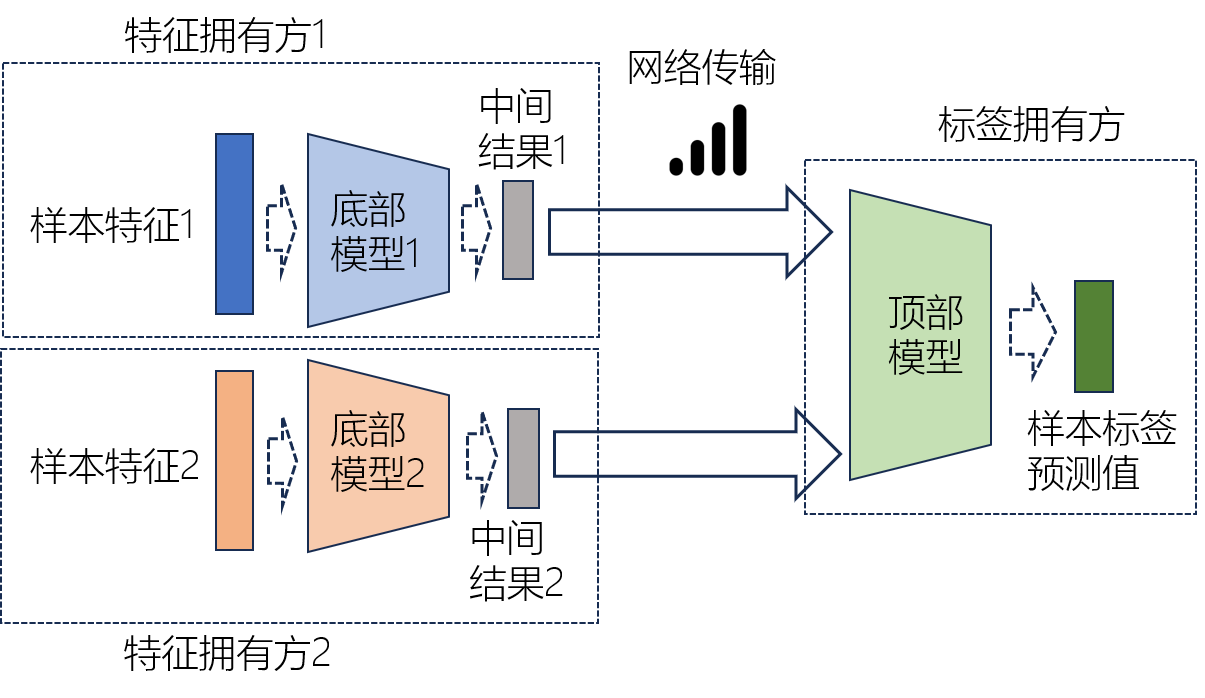
\includegraphics[width=0.8\linewidth]{Z_Resources/拆分学习示意图.png}
    \caption{拆分学习示意图}
    \label{fig:related_work:split_learning}
\end{figure}

一个简单的拆分学习例子如\autoref{fig:related_work:split_learning}所示。
%
此时纵向联邦学习有3个参与方(记作$P_1, P_2, P_3$),分别拥有样本特征第一部分($\bvec x_1$)、样本特征第二部分($\bvec x_2$)和样本标签($\hat y$)。
%
相应地,模型也被划分成了3个部分,分别是底部模型第一部分($M_{b1}$,参数记为$\Theta_{b1}$),底部模型第二部分($M_{b2}$,参数记为$\Theta_{b2}$),以及顶部模型($M_t$,参数记为$\Theta_h$)。
%
在前向传播的过程中,$P_1$和$P_2$分别本地计算得到各自的中间结果:
$
    \left(
        \bvec h_1 = M_{b1}(\bvec x_1;\Theta_1),
        \bvec h_2 = M_{b2}(\bvec x_2;\Theta_2)
    \right)
$,
然后将其发送给$P_3$(标签拥有方)。
%
$P_3$接收到$\bvec h_1, \bvec h_2$之后,将其输入到顶部模型,计算得到模型输出$y = M_t(\bvec h_1, \bvec h_2; \Theta_h)$。
%
这样便完成了一次前向传播过程。
%
%
在反向传播过程中,$P_3$通过模型的预测标签($y$)和真实标签($\hat y$),计算出损失函数$L(y, \hat y)$,并且将其对于顶部模型和中间结果的参数求梯度得到${\partial L(\hat y, y)}/{\partial \Theta_t}, {\partial L(\hat y, y)}/{\partial \bvec h_1}$ 和 ${\partial L(\hat y, y)}/{\partial \bvec h_2}$.
%
其中,前者被标签拥有方用于更新顶部模型参数,而后两者则发给相应的特征拥有方用于计算损失函数相对于底部模型参数的梯度。
%
该计算通过链式求导法则进行,以$P_1$为例:
\begin{equation}
    \dfrac{\partial L(\hat y, y)}{\partial \Theta_{b1}} = \dfrac{\partial L(\hat y, y)}{\partial \bvec h_1}\cdot \dfrac{\partial \bvec h_1}{\partial \Theta_{b1}}.
\end{equation}
%
注意,上式中的${\partial \bvec h_1}/{\partial \Theta_{b1}}$是雅可比矩阵,链式法则中的乘法也是对应的矩阵乘法运算。

拆分学习具有原理简单、实现方便、计算和通信开销小、可以适用于不同的深度学习模型等优势,因此其已经被应用于很多需要考虑数据隐私的领域,如:医疗影像分割\cite{roth2022split_unet}、边缘设备中的图像分类\cite{fagbohungbe2022split_edge_image,palanisamy2021spliteasy}、毫米波接收功率预测\cite{koda2020split_mmwave}等。

\subsection{拆分学习中的隐私问题}
虽然拆分学习具有实现简单、效率高等诸多优势,但是在训练和推断过程中,各方直接交换了中间结果和中间梯度的明文,从而存在一定的隐私泄漏风险。
%
拆分学习的隐私泄露可以分为两类:特征拥有方的隐私泄露和标签拥有方的隐私泄露。
%
下面将对这两种隐私泄露分别进行介绍。
%
\subsubsection{特征拥有方的隐私泄露}
在拆分学习的过程中,特征拥有方将底部模型产生的中间结果,也就是神经网络的隐层表征(Hidden Representation),直接发送给了标签拥有方。
%
作为输入特征经过变换的结果,隐层表征必然包含了输入特征的信息。
%
假设攻击者腐化了标签拥有方,便可以通过各种手段从隐层表征中恢复出部分输入特征的信息。
%https://www.overleaf.com/project/6564295824afdb06585a588e#
因此,近年来也有许多工作研究了拆分学习中特征拥有方的隐私泄露问题,现总结如下:
%
\begin{enumerate}
    \item 在卷积神经网络中,隐层表征直接包含了输入的信息\cite{abuadbba2020can_split}。
    由于卷积层的局域运算特性,其会保留图像本身的大致形状、轮廓等信息。
    即便经过多个卷积层后,隐层表征依然能够保留图像的整体轮廓,从而使得原始图像的数据出现一定程度的泄露。
    %
    \item 攻击者可能训练一个逆向网络从隐层表征中重构出原始输入特征~\cite{vepakomma2020nopeek,hezecheng_2019_model_inversion_attack}。
    一种简单的情况可以是,攻击者能够获取一部分泄漏的样本特征$(\bvec x_1, \cdots, \bvec x_n)$和对应的隐层表征$(\bvec h_1, \cdots, \bvec h_n)$,则最优的重构函数$R_*$可以定义为:
    \begin{equation}
        R_* = \mathop{\text{argmin}}_{R} \sum_{i=1}^n \Vert R(\bvec h_i) - \bvec x_i\Vert^2 = 
        \mathop{\text{argmin}}_{R} \sum_{i=1}^n \Vert R(M_b(\bvec x_i)) - \bvec x_i\Vert^2,
    \end{equation}
    其中,$\Vert \cdot\Vert^2$ 表示二范数平方,也可以按照具体情况换成其他的函数来度量重构效果。
    一般可以采用一个和底部模型相对应的神经网络作为重构函数,比如原始模型是是多层卷积,则$R$可以主要由反卷积(ConvTranspose)构成。
    %
    \item 如果攻击者本身拥有底部模型的参数信息,则可以采用白盒攻击的形式,优化$\bvec x'$使得$M_b(\bvec x')$尽可能接近$\bvec h = M_b(\bvec x)$~\cite{hezecheng_2019_model_inversion_attack,luoxinjian2021feature_attack}:
    \begin{equation}
    \label{eq:related_work:whitebox-reconstruction}
        \bvec x'_* = \mathop{\text{argmin}}_{\bvec x'} \Vert M_b(\bvec x') - \bvec h\Vert^2 = \mathop{\text{argmin}}_{\bvec x'} \Vert M_b(\bvec x') - M_b(\bvec x)\Vert^2.
    \end{equation}
    %
    注意到\autoref{eq:related_work:whitebox-reconstruction}可能有无穷多个解,影响重构效果。为了提高重构效果,也可以在损失函数中加入关于输入特征的先验知识。
    %
    比如输入特征是图像,则可以在损失函数中加入$\bvec x'$的总变差(Total Variance),使得重构出来的结果更接近实际图像;
    如果攻击者有同一样本的额外特征$\bvec z$,则可以将$\bvec x'$替换为$g(\bvec z)$,这里假设想要攻击的输入特征和攻击者获取的额外特征有关。
    %
    \item 在训练过程中,攻击者可以对训练目标进行修改,使得中间结果包含更多关于输入特征的信息。比如假设攻击者拥有一部分泄漏的样本特征$\{ \bvec x' \}$,
    则他可以先训练一个自编码器~\cite{kramer1991autoencoder,baldi2012autoencoders}$(f,f^{-1})$使得$f^{-1}\circ f(\bvec x')\approx \bvec x'$。
    %
    在拆分学习训练过程中,攻击者采用对抗训练的方式,使得待攻击样本的隐层表征$\bvec h = M_b(\bvec x)$与自编码器编码的泄漏样本的特征$f(\bvec x')$尽可能接近。
    %
    于是攻击者可以直接通过$f^{-1}(\bvec h)$来重构原始的输入特征~\cite{pasquini2921inference_attack_tiger}。
    %
\end{enumerate}

值得注意的是,第4种方法需要攻击者改变正常的拆分学习训练过程,而前面介绍的3种方法则不需要改变训练过程。
%
一般将主动改变训练过程的攻击者称为“主动攻击者(Active Attacker)”,反之则称为“被动攻击者(Passive Attacker)”。
%
主动攻击者往往能取得更强大的攻击效果,但是由于其对训练本身的改变,可能导致训练效果变差、训练速度变慢等问题,会更容易被检测出来,且无法在模型推断阶段进行攻击。
与此相反,被动攻击者的攻击效果会更低,但是具有更好的隐蔽性。

\subsubsection{标签拥有方的隐私泄露}
对于标签拥有方的隐私泄露,我们考虑的是攻击者腐化特征拥有方的情况。
%
标签拥有方的隐私泄露主要来源于两个方面:
\begin{enumerate}
    \item 隐层表征(中间结果)导致的标签信息泄露。
    深度学习模型学习的过程,可以看做一个将输入特征逐渐转化成标签的过程。
    因此,随着训练的进行,隐层表征会逐渐变得与标签更为相关。
    %
    许多将神经网络隐层表征可视化的工作也显示出,随着训练的进行,隐层表征逐渐按照对应的标签聚类成不同的簇;且越靠近输出的隐层表征和标签关联度越大~\cite{paulo2017visualize_hidden,pezzotti2017deepeyes,cantareira2020hidden_vector_fields}。
    %
    在这种情况下,攻击者就可以根据隐层表征来推断输入数据的标签。
    %
    即使在没有任何额外信息的情况下,攻击者也可以对隐层表征进行聚类,从而获取输入样本的类别关系~\cite{liujunlin2022clustering_attack,liujunlin2023distance_attack}。
    %
    如果攻击者能够获取少量泄漏的隐层表征和对应的标签,也可以自己训练一个顶部模型,并且获得很好的分类效果~\cite{fucong2022label_infer_attack}。
    %
    \item 隐层表征的梯度导致的标签信息泄露。
    与隐层表征类似,隐层的梯度和标签信息也呈现出非常强的相关性。
    %
    比如在二分类模型中,同类样本的梯度间的余弦相似度接近1,而异类样本的梯度间的余弦相似度则接近-1,直接暴露了样本的类别信息~\cite{oscarli2022label_defense_marvell}。
    %
    此外,也可以通过优化替代样本的梯度,使其尽可能接近攻击者获取到的梯度,从而复原出样本的标签~\cite{erdogan2022unsplit}。
    %
    具体方法如下:
    \begin{equation}
        \mathop{\text{argmin}}_{\Theta_t', \hat y'} \left\Vert \dfrac{\partial L[\hat y', M_t(M_b(\bvec x);\Theta_t')]}{\partial M_b(\bvec x)} - \dfrac{\partial L[\hat y, M_t(M_b(\bvec x);\Theta_t)]}{\partial M_b(\bvec x)} \right\Vert^2,
    \end{equation}
    其中,$\bvec x, \hat y$ 是原样本的特征和标签,而$\hat y'$是随机初始化的替代标签;$\Theta_t, \Theta_t'$分别表示原始的顶部模型参数和替代的顶部模型参数。
    通过优化替代的样本和顶部模型参数,可以恢复出样本的标签。
\end{enumerate}

标签泄露不仅仅带来了样本标签的隐私问题,同时还会泄露模型本身。
%
如上文所述,当特征拥有方腐化(Corrupted)后,它可以利用少量标签(或直接聚类生成标签),训练出顶部模型。
%
由于在模型训练的后期,底部模型的表征提取能力已经很强,固定底部模型后,攻击者很容易就可以训练出一个表现良好的顶部模型,从而得到整个完整的模型。
%
因此,这种攻击也被称为“模型补全攻击(Model Completion Attack)”~\cite{fucong2022label_infer_attack}。
%
在这种情况下,腐化的特征拥有方可以窃取几乎标签拥有方的所有资产(标签和顶部模型),从而使得拆分学习的隐私保护能力受到严重损害。


\subsubsection{总结}
%
无论是输入特征的泄露还是标签的泄露,都与许多因素有关,包括模型结构和拆分的层数。
%
显而易见的是,如果分割点靠近模型输入,则隐层表征泄漏的特征信息更多;而分割点接近模型输出,则会泄露更多关于标签的信息。
%
这也是著名的数据处理不等式(Data Processing Inequality)的推论。
%
模型的结构也对隐私泄漏的程度有很大的影响。
%
从输入特征的角度而言,
%
对于卷积神经网络,卷积层的隐层表征与输入十分相关,且很多网络的隐层维度也很高,因此很容易被攻击者重构出输入特征~\cite{abuadbba2020can_split};
%
对于全连接网络,如果隐层维度小于数据维度,则会存在无穷多组输入拥有同样的隐层表征,
这导致没有先验知识的情况下,攻击者难以获取输入特征信息;
%
基于Transformer结构的语言模型,包括时下流行的大语言模型(Large Language Model),拥有很高的隐层表征维度,并且保留了序列结构,因此攻击者也可以轻易地从隐层表征中重构出原始的输入文本~\cite{morris2023embedding_almost}。
%
从标签的角度而言,更低的隐层表征维度往往意味着更容易恢复出标签,因为高维度的特征中可能包含许多与标签无关的信息,使得攻击者更难从中提取出标签~\cite{oscarli2022label_defense_marvell,sunjiankai2022forward_embedding_protect}。


\subsection{拆分学习的隐私保护方法}
为了解决前文所述的拆分学习中的隐私泄露问题,一些研究也提出了保护拆分学习中输入特征和标签的隐私的方法,当前主要采用的方法是对隐层表征或隐层梯度进行扰动。

首先介绍对隐层表征进行扰动,使其与输入特征或标签特征不相关的方法。
%
由于隐层表征、输入特征、标签的维度可以是任意的,因此常用的皮尔逊相关性(Pearson Correlation)并不适用。
%
因此现有工作主要采用距离相关性来衡量隐层表征和输入特征、标签的相关性~\cite{vepakomma2020nopeek,sunjiankai2022forward_embedding_protect}。
%
距离相关性(Distance Correlation)~\cite{szekely2007dcor,szekely2009brownian_dcor}是一种特殊的相关性度量,可以度量不同维度的随机向量之间的相关性,并且可以度量非线性的相关性,距离相关性为0当且仅当两个变量是无关的(互信息为0)。
%
使用距离相关性来保护输入特征或标签信息的损失函数可以写为:
\begin{equation}
    L' = L_0 + \alpha \text{Dcor}(H, X) + \beta \text{Dcor}(H, Y),
\end{equation}
其中,$\text{Dcor}(\cdot, \cdot)$表示距离相关性,$X,H,Y$分别表示当前批次的输入特征、拆分层表征和标签,$\alpha,\beta$则用于控制扰动程度。
%
注意到,此处的距离相关性计算是通过批样本的经验分布(Empirical Distribution)进行估计的,因此需要较大的批大小(Batch Size),否则估计值会出现较大的误差。
%

针对隐层梯度泄露标签信息的情况,Marvell方法~\cite{oscarli2022label_defense_marvell}通过最小化正样本和负样本之间的隐层梯度间的KL散度来保护样本的标签信息。
%
当标签拥有方计算出隐层梯度$g = \partial L/\partial \bvec h$时,它会对其加入一个正态分布的噪声$D \sim \mathcal N(0, \Sigma_D)$,然后将其发给特征拥有方。
%
具体的优化问题可以写做:
\begin{equation}
\begin{split}
\label{eq:related_work:marvell}
    & \min_{\Sigma_D^+,\Sigma_D^-} \text{KL}\left[\mathcal N(\mu_g^+, \Sigma_g^+ + \Sigma_D^+)\Vert\mathcal N(\mu_g^-, \Sigma_g^- + \Sigma_D^-)\right],
    \\
    & \text{s.t.}\quad p\text{tr}(\Sigma_D^+) + (1-p)\text{tr}(\Sigma_D^-) \le P,
\end{split}
\end{equation}
这里假设正样本和负样本的原始的隐层梯度也分别满足正态分布$\mathcal N(\mu_g^+, \Sigma_g^+)$和$\mathcal N(\mu_g^-, \Sigma_g^-)$,
而$\Sigma_D^+,\Sigma_D^-$则分别是给正样本和负样本的隐层梯度家的噪声的协方差矩阵。
%
约束条件中的$p$和$1-p$分别代表正样本和负样本的频率,$P$表示设定的噪声大小的平均值上限,用于控制噪声的规模,防止添加的噪声太大。
%


上述对隐层表征和梯度的扰动方法均存在一些缺陷。
%
在隐层表征维度高的情况下,距离相关性的估计会变差,从而使得其保护效果大幅度降低~\cite{erdogan2022unsplit}。
%
而Marvell方法~\cite{sunjiankai2022forward_embedding_protect}虽然对梯度进行了扰动,并不能防止从隐层表征直接推出样本标签的情形,
同时该方法也仅适用于二分类场景。
%
因此,如何保护拆分学习过程中的特征和标签隐私,依然是个极具挑战性的问题。


\subsection{拆分学习的效率提升}
相对于基于密码学方法的隐私保护机器学习,拆分学习具有较小的开销,因为拆分学习仅仅是在明文计算的基础上,传输隐层表征和隐层梯度,并未引入额外的计算。
%
但是考虑到许多神经网络的隐层尺寸较大,因此在通信效率方面,拆分学习依然存在可以优化的空间。
%
一种简单的思路是将稀疏(Sparsification)和量化(Quantization)方法引入拆分学习,对隐层表征和隐层梯度进行压缩,从而减少拆分学习训练和推断过程中的通信量。
%

\textbf{稀疏化:}
对一个向量(或矩阵、张量)进行稀疏化,指的是将其(绝对值)较大的元素保留,而将其绝对值较小的元素丢弃,即设置为0。
%
稀疏化有效性基于“较大的元素在计算过程中较为重要,而较小的元素在计算过程中可以忽略”这一假设。
%
稀疏化之后,数据的传输格式也会发生变化。一种简单的做法是将数据以“(下标,值)”的形式进行编码。假设原有的数据位数为$L$(如对于32位浮点数$L=32$),数据的总量为$N$,稀疏率为$p$,则简单的下标-值编码方法可以实现压缩比率(压缩后大小/压缩前大小)为:
\begin{equation}
    \text{压缩比率}=\dfrac{pN(L + \lceil \log_2N \rceil)}{NL} = p(1 + \dfrac{\lceil \log_2N \rceil}{L}).
\end{equation}
为了提高压缩比率,可以采用更加先进的数据压缩方法,如经典的Huffman编码~\cite{huffman1952}可以直接应用于稀疏化后的数据(的二进制表示)上。
%
更为适合稀疏化的编码为对下标的差值(Run-length)序列进行Golomb编码~\cite{gallager1975golomb}。
%
如果在一批数据中,每个下标被稀疏化的概率是均等的,则Golomb编码具有最小的期望压缩比率,大约可以在下标-值编码的基础上再减少一半~\cite{sattler2019sparse_binary}。
%
值得注意的是,采用编码方案虽然减少了通信开销,但是也会带来一定的计算开销。


\textbf{量化:}
量化指的是降低数据的精确度,使用较少的比特位保留数据,在尽可能保证数据的准确性的情况下,压缩其存储空间。
%
一般的机器学习模型的训练或推断采用的都是32位浮点数,通过量化的方式,可以将模型的权重、模型计算的中间结果等压缩到更低位数(如8位,4位,甚至1位),从而减少模型大小或降低模型计算过程中的内存开销和计算开销~\cite{zhou2016dorefa,banner2018_8bit,yang2019quantization}。




利用稀疏化和量化减轻通信量的方法,在分布式计算、横向联邦学习领域被广泛应用~\cite{wen2017terngrad,sattler2019sparse_binary}。
%
此时,稀疏化和量化可以同时被应用在表征和梯度上,从而减少了每轮训练过程中的通信量开销。
%
虽然稀疏化和量化导致梯度不准确,由于使用随机梯度下降(Stochastic Gradient Descent)优化时,批样本梯度本身有一定噪声,甚至被认为对收敛(Convergence)和泛化(Generalization)是有益的~\cite{hardt2016sgd,goyal2017sgd_imagenet,chaudhari2018sgd}。
%
同时,相关研究也表明,稀疏化和量化并未对模型最终的结果有显著影响,而训练到一个较高准确度的通信量也显著小于常规训练的通信量~\cite{aji2017sparse,sattler2019sparse_binary,wen2017terngrad}。

%
但是拆分学习作为一个较新的领域,其通信效率提升的研究相对较少。
%
Castiglia等人~\cite{castiglia2022compressed_vfl}研究了基本的Top-$k$稀疏化、(标量)量化以及向量量化(Vector Quantization)在拆分学习中的应用,并且证明了其收敛性。
%
具体而言,拆分学习训练时的前向传播过程被更改为
\begin{equation}
\label{eq:split-compress}
    Y = M_t(\mathsf{Compress}[M_b(X)]),
\end{equation}
%
其中,$M_t$表示顶部模型,$M_b$表示底部模型,$X, Y$ 表示输入特征和模型预测值,$\mathsf{Compress}$表示压缩操作(如稀疏、量化)。
%
尽管收敛性得到证明,但是该文采用的压缩方法最多只能将压缩率降低到1/16,且常规的稀疏和量化(除了向量量化外)对模型最终的效果有较明显的降低。
%
此外,该方法只适用于训练场景,并未考虑推断场景,并且要求公开的顶部模型让各个参与方执行块坐标下降法(Block Coordinate Descent)对自身的参数进行优化。

也有部分研究采用异步更新的方式提高拆分学习的通信效率,其方法包括底部模型多轮本地更新~\cite{fu2022cache_vfl}或是顶部模型多轮本地更新~\cite{chen2021async_split}。
%
这些方法同样针对的是拆分学习训练的场景,并不能应用于推断阶段。
%
此外,Ayad等人~\cite{ayad202vfl}提出使用自编码器压缩中间表征,也就是将\eqref{eq:split-compress}中的$\mathsf{Compress}$替换为一个自编码器,从而实现训练和推断过程中的通信优化。
%
但是该方法需要针对特定模型定制自编码器,并非一种通用的方法。
\section{基于密码学的隐私保护机器学习}
纵向联邦学习可以看作是特定的一类隐私计算问题,即:在保护数据和模型参数的情况下进行模型的训练和推断,因此也可以通过基于密码学的安全多方计算(Secure Multiparty Computation)来实现。
%
\begin{definition}[安全多方计算]
    有$n$个参与方$P_1, \cdots, P_n$与各自的输入$X_1, \cdots, X_n$,以及一个公共函数$f$,安全多方计算指的是各方根据指定的协议交互计算出$Y= f(X_1, \cdots, X_n)$($Y$可以是公开的或是被指定的参与方获得,两种定义是等价的),同时保护各方输入的隐私。
\end{definition}
%
注意安全多方计算的定义隐含了安全性设定(Security Setting),也就是对于各个参与方行为的限制条件,包括:各个参与方忠实执行计算协议但是同时利用自己获取到的一切信息,称为半可信(Semi-honest)安全性设定,以及参与方可能存在不遵守计算协议的情况,称为恶意(Malicious)安全性设定,以及在上述两种情况下部分参与方共谋(Collusion)的情况。
%
复杂的安全性设定可能导致极为复杂的协议设计和安全性证明。
%
本文遵循一般隐私保护机器学习中的半可信安全性设定。
%
%


安全多方计算协议往往基于几种特定的密码学原语来实现,包括秘密分享(Secret Sharing)、同态加密(Homomorphic Encryption)、混淆电路(Garbled Circuits)等。
%
下面对此进行简要介绍。
%


\textbf{秘密分享}:
秘密分享~\cite{shamir1979share}指的是把一个值分享给多个参与方,其中一定数量的参与方合作才能恢复出该值。
%
具体而言,
%
$(t,n)$-秘密分享指的是将一个值$x$分享给$n$方$P_0, \cdots, P_{n-1}$,其中$P_i$得到的值记作$\langle x \rangle_i$。
%
至少要$t$个参与方一起,才能恢复出$x$的值。低于$t$个参与方则无法得到任何关于$x$的信息。
%
常用的秘密分享包括两方加法分享(Additive Sharing)以及两方布尔分享(Boolean Sharing),这两种分享分别把一个数$x$拆分成两个随机数相加($x = \langle x \rangle_0 + \langle x \rangle_1$)或是两个随机数(按位)异或($x = \langle x \rangle_0 \oplus \langle x \rangle_1$)。
%
在秘密分享的情况下,进行加法(异或)只需各方本地运算,但是进行乘法(异与)较为复杂,一般可以采用离线(Offline)计算的Beaver三元组进行~\cite{beaver1992efficient},即:在获得具体的输入前,两方通过一定方法计算出一组秘密分享的随机数$(u,v,w)$满足$uv = w$。
%
一般可以使用同态加密、不经意传输(Oblivious Transfer)等手段,在三方场景下,可以使用一个半可信第三方分发从而提高离线计算的效率。
%
注意秘密分享一般在有限域上进行,如:加法分享在模$N$的整数环$\mathbb Z_N$进行,布尔分享按照定义在$\mathbb Z_2$进行)。
%
此时各方所获取到的值都是在有限域上均匀分布的随机数,与实际值无关,因此实现信息论安全(Information-Theoretic Security)。


\textbf{同态加密}:
同态加密是一类特殊的加密算法,其支持在密文上进行一定的计算,使得解密的结果和明文计算一致。
%
令某种加密系统的加密函数为\textsf{Enc},解密函数为\textsf{Dec}。
%
如果对于某个定义在明文上的运算符$\mathsf{OP}_P$,存在密文上的运算符$\mathsf{OP}_C$,使得对于任意明文$X, Y$都满足:
\begin{equation}
    \textsf{OP}_P(X, Y) = \mathsf{Dec}[\mathsf{OP}_C (\mathsf{Enc}[X], \mathsf{Enc}[Y])],
\end{equation}
%
则称该加密系统可以同态地计算$\mathsf{OP}_P$的运算。
%
注意$\mathsf{OP}_P$ 往往不等于 $\mathsf{OP}_C$。
比如,Paillier同态加密支持明文加法,即:$\mathsf{OP}_P=$`$+$',但是对应的密文运算是乘法,也就是$\mathsf{OP}_C=$`$\times$'。
%
同态加密按照支持的运算的不同,一般可以分为半同态加密(Partial Homomorphic Encryption)和全同态加密(Fully Homomorphic Encryption)。
%
半同态加密支持一种同态运算,如加法或乘法,分别可以称为加同态加密和乘同态加密。
%
全同态加密同时支持加法或乘法。
%
除此之外,还有分级(Leved)全同态加密,其只支持一定次数多乘法运算。
%
当前常用的同态加密包括Paillier加同态加密~\cite{paillier1999},其定义域为大整数;BFV/BGV全同态加密~\cite{2012bfv1,2012bfv2,2014bgv},其定义域为整系数多项式;以及CKKS全同态加密~\cite{ckks2017},其定义域是实系数多项式,并且运算过程会产生一定的误差。


\textbf{混淆电路}:
混淆电路由姚期智院士于1986年提出~\cite{yao1986gc},是一个两方安全计算协议,可以用于计算任意布尔电路。
%
混淆电路通过对原始电路的逻辑门进行“混淆”得到,具体而言,每个门的输入和输出都变成了随机数,因此无法根据混淆后的电路的输入、输出以及中间值,获取关于原始电路输入输出值的任何信息。
%
混淆电路的执行过程可以表示为:给定一个公开函数$f$,某方(这里设为$P_0$)产生一个布尔电路$C$,然后对其进行混淆得到混淆电路$C^G$,并发送给另一方(这里设为$P_1$);同时,$P_0$自身的输入$X_0$ 混淆后得到 $X_0^G$
%
同时,$P_1$和$P_0$ 执行不经意传输协议,获取$P_1$输入的混淆值 $X_1^G$。
%
然后$P_1$可以根据混淆输入计算出混淆输出:$Y_G = C_G(X_0^G, X_1^G)$,将其返还给$P_0$后,$P_0$根据自身维护的混淆表得到实际的输出值。
%
混淆电路只需要常数轮的通信即可计算任何门电路的值,但是因为电路中的每个布尔值都转化成了高位的随机数,会消耗大量通讯流量;由于涉及密码学计算,也有较大的计算开销。
%
混淆电路发展至今有多种优化方案提出,包括Free-XOR~\cite{kolesnikov2008free_xor},HalfGate~\cite{zahur2015halfgate}等,降低了通讯和计算开销。
%

除去以上介绍的几种密码学技术,多方安全计算还可以包含其他技术,以及一些定制化的计算协议。
%
下文将对部分主要的基于密码学的隐私保护机器学习研究进行介绍。


\subsection{基于单一密码学技术的隐私保护机器学习}
本节对采用单一密码学技术来实现隐私保护机器学习的相关工作进行介绍。
%
这些工作基于两方的隐私保护机器学习场景,如MLaaS(Machine Learning as a Service),即:用户提供数据,服务方提供机器学习模型。
%

\textbf{基于同态加密}:
2016年微软提出CryptoNets~\cite{gilad2016cryptonets},率先通过同态加密实现神经网络的推断。
%
由于神经网络的权重和输入都被加密,因此这种方法可以实现安全的神经网络推断。
%
CryptoNets采用了YASHE加密算法~\cite{bos2013yashe},这是一种分级同态加密算法,可以支持一定次数的乘法运算、
%
由于同态加密仅仅支持加法和乘法运算,因此CryptoNets将神经网络中的非线性激活函数替换成了平方函数,然后再明文上训练得到模型权重。
%
该方法需要花费数分钟和300Mb左右的流量对MNIST数据集中的一张图片进行分类。
%
%
一些未正式发表的工作~\cite{hesamifard2017cryptodl,chabanne2017pp_dnn}对CryptoNets进行了改进,包括使用更加精确的多项式拟合激活函数、将同态加密算法换为BGV或CKKS等更高效的算法,以及优化同态加密的密文打包技术等。
%
Zhou等人通过将卷积神经网络的权重二值化,实现了更高效的基于全同态加密的神经网络推理~\cite{zhoujunwei2020binary_encrypted_nn}。

\textbf{基于混淆电路}:
DeepSecure框架~\cite{rouhani2018deepsecure}将神经网络模型转化为布尔电路,从而实现隐私神经网络推断。
%
为了提高效率,该框架减少了各类电路中的非异或门数目,从而适配Free-XOR算法。
%
该框架运算速度高于CryptoNets,但是带来了更高的通讯开销。
%
实验表明,一个简单的全连接网络的推断消耗800MB左右的流量。
%
XONN框架~\cite{riazi2019xonn}将二值神经网络(Binary Neural Network)与混淆电路结合,将内积运算转变为异或运算,从而极大地提高了安全推断的效率。


\subsection{基于混合技术的隐私保护机器学习}
为了提高隐私保护机器学习的效率,现有的隐私保护机器学习框架大多将多种密码学技术混合,为机器学习中不同的算子找到最佳的密码学技术。
%

\textbf{两方框架}:
ABY框架~\cite{demmler2015aby}提出将算数秘密分享、布尔秘密分享以及YAO分享(基于混淆电路~\cite{yao1986gc}的两方分享,一方持有混淆值和真实值的对照表,另一方持有混淆电路和混淆值)融合,并且涉及协议对三种分享状态的值进行相互转化,从而为特定的计算任务找到最适合的混合计算协议。
%
SecureML框架~\cite{mohassel2017secureml}将算数秘密分享和混淆电路结合,实现了逻辑回归的推断和训练。
%
其还使用分级同态加密和不经意传输对算数秘密分享的Beaver三元组~\cite{beaver1992efficient}的离线生成进行了优化,并且将Sigmoid函数表示为分段线性函数,通过混淆电路(计算当前值落在哪一段)和算数秘密分享融合来提高计算效率。
%
MiniONN框架~\cite{liujian2017minionn}将秘密分享和混淆电路进一步应用于神经网络推断中,并且使用分段的Spline插值来拟合激活函数,以及采用SIMD(Single Instruction Multiple Data)技术加速了Beaver三元组的生成,从而提高了隐私神经网络的模型准确率和效率。
%
Gazelle框架~\cite{juvekar2018gazelle}使用优化的基于格密码的同态加密(BFV加密~\cite{2012bfv1,2012bfv2})直接加速安全矩阵乘法计算,而非用于产生三元组,从而极大提高了通讯效率;同时采用混淆电路来计算ReLU、最大池化(Max Pooling)等非线性运算。
实验结果表明Gazelle的性能甚至大幅度优于需要依赖第三方的Chameleon框架。
%
Delphi框架~\cite{mishra2020delphi}基于Gazelle框架进行了改进,将同态加密的安全乘法计算用于离线计算Beaver三元组,并利用了神经网络推断过程中权重不变的特性减少了在线的开销;同时将ReLU激活函数替换成二次函数以降低开销。
%
CryptFlow2框架~\cite{rathee2020cryptflow2}基于秘密分享,采用同态加密和不经意传输实现安全乘法,并且新设计了高效的基于不经意传输的安全比较和除法协议,将两方的隐私保护机器学习推广到ResNet等大型模型中。
%
Cheetah框架~\cite{huang2022cheetah}进一步对基于同态加密的神经网络线性运算以及基于不经意传输的ReLU激活函数等非线性运算进行优化。
%si
SIRNN框架~\cite{rathee2021sirnn}通过查真值表的方式计算指数函数,进一步对神经网络中Softmax等非线性函数进行了优化。

\textbf{三方框架}:
Chameleon框架~\cite{riazi_2018_chameleon}混合秘密分享、GMW协议和混淆电路协议进行神经网络计算,在离线阶段使用了可信硬件作为第三方,并采用相关随机性(Correlated Randomness)在各方生成相同的随机数,提高了Beaver三元组产生的效率。
%
ABY3框架~\cite{mohassel2018aby3}基于ABY框架~\cite{demmler2015aby},将秘密分享、布尔分享和混淆电路推广到三方计算的场景以提高效率,并对乘法截断进行了改进。
%
SecureNN框架~\cite{wagh2019securenn}采用了两方秘密分享并且使用第三方来产生Beaver三元组,同时基于比较的布尔运算电路设计了高效的三方安全比较协议,实现了高效的隐私神经网络推断。
%
CryptFlow~\cite{kumar2020cryptflow}是一个支持两方和三方协议的开源框架,其两方协议采用的是ABY协议,而三方协议基于SecureNN框架,对其卷积操作的Beaver三元组进行了优化,同时使用相关随机性来进一步降低通信量;该框架还提供了基于可信执行环境(Trusted Execution Environment, TEE)的恶意安全转换机制,可以将半可信安全的协议转换为恶意安全的协议。
%
Crypten框架~\cite{knott2021crypten}基于秘密分享和GMW协议实现安全的深度学习,并且提供了类似Pytorch风格的接口,使得非密码学专业研究者也可以进行隐私保护机器学习。
%
Falcon框架~\cite{wagh2021falcon}基于ABY3和SecureNN进行了改进,优化了比较协议。
%
AriaNN框架~\cite{ryffel2021ariann}提出使用函数秘密分享(Function Secret Sharing)来计算比较函数,将其降低到仅需一轮通信轮次。

\subsection{其他相关研究}
除了设计安全多方计算框架之外,也有一些其他关于提高基于密码学的隐私保护机器学习效率的研究。
%
比如,
Dalskov等~\cite{dalskov2020secure_q8}研究了将量化(Quantization)技术应用于隐私保护机器学习,将神经网络量化到8比特,并在多个现有的隐私保护机器学习框架上进行了测试。
%
此外,也有许多对于非神经网络的专用机器学习模型进行隐私保护的研究,如树模型~\cite{wu2020vf_tree,fang2021secure_xgb,lu2023squirrel}、聚类模型~\cite{bunn2007secure_kmeans,wu2020secure_kmeans}、矩阵分解~\cite{nikolaenko2013ppmf,kim2018ppmf}等。
%
这些方法往往基于已有的同态加密、混淆电路、多方安全计算协议等技术,对于特定的机器学习模型进行设计和优化。
%


2023年起,随着ChatGPT的出现,大语言模型在工业界和学术界产生了巨大的影响。
%
而大模型的参数量和计算量都极为巨大,即使是明文推断的情况下也对硬件有较高要求,因此对基于密码学的隐私保护机器学习提出了新的挑战。
%
Iron Transformer~\cite{hao2022iron},MPCFormer~\cite{li2022mpcformer},SecureTLM~\cite{chen2024securetlm},PrivFormer~\cite{akimoto2023privformer}等框架在之前研究的基础上,采用同态加密、秘密分享、多项式拟合ReLU、使用特定结构的模型等方法,实现了Transformer模型的隐私保护推断。
%
针对参数量高达数十亿的大语言模型,最近也有研究基于已有的ABY3协议或Cheetah框架进行~\cite{dong2023puma,lu2023bumblebee,hou2023ciphergpt}。
目前这些方案在生成单个输出单词时需要至少进行数十GB的流量传输,在理想环境下也需要数分钟的计算时间,因此依然难以用于实际应用。




\section{密码学与非密码学混合的隐私保护机器学习}
考虑到基于密码学的隐私保护机器学习框架往往开销巨大且实现困难,也有许多研究尝试将密码学和非密码学方法进行融合,从而实现更高效的隐私保护机器学习。
%

一种方法是将同态加密和其他方法结合,将线性计算部分用同态加密实现,而非线性激活函数部分则用明文实现,其计算流程大致可以表示为
\begin{equation}
    \llbracket \bvec y \rrbracket = W \otimes \llbracket \bvec x \rrbracket  + \llbracket \bvec b \rrbracket, \quad \bvec x' = f(\bvec y),
\end{equation}
其中,$\llbracket \cdot \rrbracket$表示加同态加密的密文,$\otimes$ 表示明文和密文的同态乘法,其结果为乘积的密文,$f$表示激活函数,$\bvec x, \bvec x'$分别表示当前层和下一层的输入。
%
GELU-Net算法~\cite{zhangqiao_2018_gelu_net}利用同态加密实现了两方的安全神经网络推断。
该算法假设用户拥有同态加密的私钥。
对于神经网络的每一层,用户将数据上传至服务器,服务器执行同态乘法运算,得到加密的结果后返回给用户,用户再计算非线性的激活函数值。
%
该方法虽然保护了用户的隐私,但是若用户多次进行查询,即可通过对多个输入$\bvec x_i$和输出$\bvec y_i$ 解线性方程组$(W\bvec x_i + b = y_i)$,恢复出神经网络的权重。
%
BAYHENN算法~\cite{xiepeichen_2019_bayhenn}类似GELU-Net,区别在于其采用贝叶斯神经网络来保证模型的隐私。
在贝叶斯神经网络中,模型的权重是随机变量,使得根据输入和输出学习权重转换成一个“噪声学习(Learning With Errors)”问题~\cite{regev_2010_lwe},而该问题被证明是一个困难问题。
%
然而后续研究~\cite{wong_2020_lwe_model}指出,BAYHENN和GELU-Net的安全性都存在问题,很容易被攻击者通过选取特定输入的方式窃取模型参数

此外,还有一些研究通过结合拆分学习和密码学方法,提高了隐私保护机器学习的效率。
Zhou等~\cite{zhou_2022_codesign}提出在多方的纵向联邦学习中使用秘密分享计算神经网络的第一个全连接层,此后在服务器上明文计算。
Chen等~\cite{chen2020vertically}将该方法进一步扩展到图神经网络~\cite{defferrard_2016_gcn,hamilton_2017_graphsage,wuzonghan_2020_gnn_survey}中。
%
BlindFL框架~\cite{fu2022blindfl}将纵向联邦学习的底部模型拆分层使用密码学方法计算,同时明文计算底部模型的其他层和顶部模型。
%
这些方法在一定程度上权衡了效率和隐私,相比于传统的拆分学习,其一般只暴露多个底部模型产生的联合表征而非单一参与方底部模型的输出。
%
但是由于中间结果的暴露,其依然面临着较大的隐私泄漏风险,存在着被逆向攻击的可能性~\cite{hezecheng_2019_model_inversion_attack,abuadbba2020can_split,luoxinjian2021feature_attack,erdogan2022unsplit,qiupengyu_2023_label_selling_you_out}。

综上所述,当前密码学和非密码学方法混合实现隐私保护机器学习的研究仍然处于起步阶段,面临着安全性方面的许多挑战。
%

    \chapter{基于随机Top-$k$算法的拆分学习效率优化}
\label{chap:randomized_topk}

拆分学习是一种简单的隐私保护机器学习方法,其适用于纵向联邦学习和隐私推断的场景。
%
在拆分学习中,各方交换模型的中间表征或梯度,实现多方的推断和训练。
%
尽管拆分学习的效率远高于基于密码学的隐私保护机器学习方法,但是其效率依然存在进一步优化的空间。
%
本章探索了拆分学习通信效率的优化方法,对稀疏、量化、缩小拆分层等方法进行了研究,从收敛和泛化两个角度进行优化,最终提出随机Top-$k$稀疏化方法,提高了拆分学习的通信效率。
%

\section{研究背景}
随着社会的数据隐私保护意识的提升和相关法律法规的出台,许多隐私保护机器学习方法被提出。
%
拆分学习~\cite{vepakomma2018split,poirot2019split}作为纵向联邦学习~\cite{liu2024vertical}的一种主要方法,有着效率较高、实现简单的优势,因此获得了工业界和学术界的广泛关注~\cite{palanisamy2021spliteasy,koda2020split_mmwave,fagbohungbe2022split_edge_image,roth2022split_unet}。
%


\begin{figure}[htbp]
    \centering
    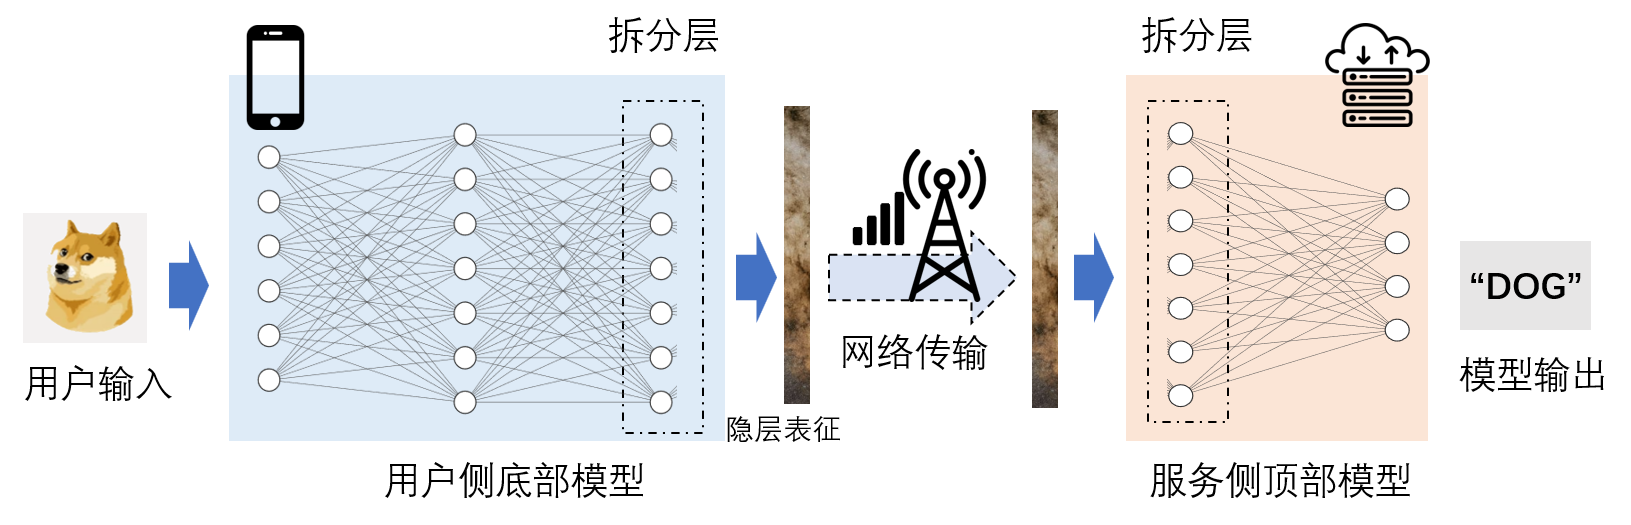
\includegraphics[width=\linewidth]{Z_Resources/随机topk_两方拆分学习示意图.png}
    \caption{两方拆分学习推断示意图}
    \label{fig:randomized_topk-split_example}
\end{figure}

拆分学习的思想是把模型拆分成多个部分分发给各个参与方,各方以交换中间结果的方式进行模型训练和推断,从而实现一定程度上的隐私保护。
%
\autoref{fig:randomized_topk-split_example}显示了一个典型的两方拆分学习的推断场景,我们假设用户具有输入数据,而服务器拥有一个分类模型。
%
进行拆分学习的推断时,用户拥有底部模型,而服务器拥有顶部模型。用户将输入输入底部模型获得隐层表征后,通过网络传输给服务器,然后将其输入顶部模型,从而得到最终的模型预测值。
%
在此过程中,用户只暴露了输入数据的隐层表征,因此其原始输入获得了一定的保护;而服务器只暴露了底部模型而非完整模型,因此模型的隐私也在一定程度上得到了保护。
%
虽然拆分学习的效率相对于密码学方法很高,但是由于拆分学习训练过程中依然需要在每一轮传输隐层特征和梯度,考虑到许多深度学习模型的隐层空间较大,因此拆分学习在通讯效率上依然存在可以优化的空间。
%



本文主要关注类别数量多的深度学习模型场景。
%
分类模型往往可以拆分为特征抽取器和分类器两个部分,其中,特征抽取器的结构较为复杂,可以包含卷积层、长短期记忆层等;而分类器可能是一层简单的全连接层。
%
但是在类别数量众多的情况下,分类器往往包含了模型的大部分参数,如:
%
推荐系统模型~\cite{jannach2017gru4rec,kang2018sasrec}的最后一层可能包含了所有商品的嵌入向量(Embedding Vector);
%
人脸识别模型~\cite{parkhi2015deepface}的最后一层可能包含了所有用户的人脸对应的嵌入向量。
%
在这种情况下,若简单地将整个模型部署到用户侧,既会占用大量的用户侧存储空间,也会带来模型隐私泄露的风险。
%
因此,在这种情况下,就需要采用拆分学习的方式来提高效率,同时保护用户输入和模型参数的隐私。

当前关于纵向联邦学习通讯压缩的研究相对较少,仅有对基础压缩算法的收敛性分析~\cite{castiglia2022compressed_vfl}、拆分层嵌入自编码器~\cite{ayad202vfl}等,前者仅考虑了基本的压缩方法且只应用于训练阶段,而后者只针对拆分学习的一个特定场景。
%
关于提升横向联邦学习的通讯效率的工作则较多,包括了加快收敛速度~\cite{karimireddy2020scaffold,reddi2020fed_opt}、压缩每一轮传输的梯度值~\cite{wen2017terngrad,aji2017sparse,sattler2019sparse_binary}等。
%
前者并不适用于拆分学习,因此本文主要研究如何压缩拆分学习训练和推断过程中传递的中间结果或中间梯度信息。
%


\section{压缩方法初步研究}
本节介绍了几种基础的可以对拆分学习的通信量进行压缩的方法,包括缩小拆分层、Top-$k$稀疏、量化拆分层、使用L1损失函数诱导稀疏,并对各方法进行初步分析。
%
在以下的分析中,我们将拆分学习的底部模型记作$M_b$,顶部模型记作$M_t$,输入、中间结果、输出分别记作$X, H, Y$。
我们使用$d$表示初始的拆分层的维度,$k$表示拆分层压缩后的维度。


\textbf{缩小拆分层}:
在拆分学习中,每一轮训练或推断都会传输拆分层(Cut Layer)的表征以及(训练时)梯度。
%
因此,缩小拆分层的大小可以直接减少拆分学习每一轮的通信量。
%
假设1个全连接网络的隐层维度分别是1000(输入)-100(第1层)-100(第2层/拆分层)-10(输出层),则每一轮前向传播需要传输100个数值;若把拆分层维度缩小到10,则只需要传输10个数值。
%
同样地,在反向传播过程中,也只需要传输10个梯度值。
%
因此,这种方法可以削减90\%的每轮通信量。

\textbf{量化拆分层}:
量化指的是将较高比特位的值(如32位浮点数)转化为较小比特位的近似值(如16位浮点数,4位整数,甚至1位的0/1布尔值)~\cite{zhou2016dorefa,banner2018_8bit,yang2019quantization}。
%
其在神经网络中被广泛应用于减少计算和存储开销。
%
通过对拆分层的值以及梯度进行量化压缩,也可以减少拆分学习训练和推断过程中的通信量。
%
本文考虑最常用的等距均匀量化(Uniform Quantization),对于一个隐层向量$\bvec{h} = (h_1, \cdots, h_d)$,将其量化为 $b$ 比特的量化方法为:
\begin{equation}
    \bvec{h}^C = \mathsf{Compress}(\bvec{h}) = \left( \left\lfloor \dfrac{h_1 - h_\text{min}}{h_\text{max} - h_\text{min}} \cdot  2^b \right\rfloor, \cdots, \left\lfloor \dfrac{h_n - h_\text{min}}{h_\text{max} - h_\text{min}} \cdot 2^b \right\rfloor \right),
\end{equation}
其中,$h_\text{min}$ 和 $h_\text{max}$ 分别表示向量$\bvec{h}$中的最小值和最大值。
%
而解压缩的过程则可以表示为:
\begin{equation}
    \bvec{h}' = \mathsf{Decompress}(\bvec{h}^C) = \left(\cdots, h_\text{min} + \big(h^C_i + \dfrac12 \big) \big(\dfrac{h_\text{max} - h_\text{min}}{2^b}\big), \cdots \right).
\end{equation}
% 
尽管量化压缩可以应用于前向传播的隐层值和反向传播的梯度值,但是在实验中我们发现,如果将量化压缩同时应用于前向传播和反向传播,会带来严重的模型效果损失。
%
考虑到本文主要关注拆分学习推断过程中的通信压缩,因此只将量化压缩应用于反向传播的隐层梯度中。

\textbf{Top-$k$稀疏化}:
Top-$k$稀疏化指在向量中只保留$k$个绝对值最大的元素,而将其他元素置为0。
%
在这种情况下,只需要传输$k$个元素的值和下标。
%
如果在前向传播中应用了Top-$k$稀疏化,则较小的$d-k$个元素没有参与顶部模型的计算,因此在反向传播过程中也无需传播这$d-k$个元素的信息。
%
Top-$k$稀疏化可以自然地同时应用于前向传播和反向传播~\cite{jayakumar_2020_topkast}。
%

\textbf{L1正则化}:L1正则化通过L1损失来诱导稀疏性,被广泛应用在不同的机器学习领域~\cite{tibshirani1996lasso,wright2008sparse_face,yin2012kernel,hoefler2021sparse_deeplearning}。
%
具体来说,在拆分学习的训练过程中,我们在原有的损失函数上加入一个对于拆分层表征向量的L1损失:$L' = L + \lambda \sum_{i=1}^d |h_i|$。
%
其中,$\lambda$用于控制稀疏化的强度,越大的$\lambda$会导致越高的稀疏性,但是同时也会降低模型训练的效果。
%
由于L1正则化需要在训练过程中逐渐实现稀疏化,因此其稀疏化只适用于模型的推断阶段,此时我们可以将拆分层表征中接近0的元素删除,类似Top-$k$稀疏化来传播绝对值较大的值和对应的下标。
%


我们将各种方法对应的压缩比率(压缩后大小/压缩前大小)总结在表 \ref{tab:randomized_top-k:compression_ratio}中。
%
对于Top-$k$即L1稀疏化,我们未考虑对下标进行压缩。
%
表中 $N$ 表示初始值的比特位数,一般为32,$k$表示保留的元素的个数。

\begin{table}[h]
    \centering
    \begin{tabular}{ccc}
    \toprule
    \multirow{2}{*}{压缩方法} & \multicolumn{2}{c}{压缩比率} \\ 
    \cmidrule(lr){2-3}
            & 前向传播 & 反向传播 \\ \midrule
    拆分层缩小     & $k/d$       & $k/d$ \\
    $b$比特量化    & $b/N$    & 1 \\
    Top-$k$稀疏化  & $k/d\cdot (1 + \lceil \log_2 d \rceil/N)$ & $k/d$ \\
    L1正则化       & $k/d\cdot (1 + \lceil \log_2 d \rceil/N)$ & 1 \\
    \bottomrule
    \end{tabular}
    \caption{不同压缩方法的压缩比率}
    \label{tab:randomized_top-k:compression_ratio}
\end{table}
\section{随机Top-$k$算法}
\label{sec:randomized_topk:method}
本章节将提出随机Top-$k$算法,其优势来自于两个方面:
(1)从模型泛化(Generalization)角度,Top-$k$稀疏化优于缩小拆分层,因为同等压缩比率下,Top-$k$稀疏化能够提供更大的表征空间和决策边界大小。
(2)从模型训练和收敛的角度,Top-$k$稀疏化会导致部分神经元训练困难,导致收敛变慢,并且无法完全利用表征空间,从而降低其泛化性能上的优势。
%
基于以上两个观察,我们通过在Top-$k$稀疏化中加入随机扰动的方式,解决了第二点的部分神经元训练困难问题,从而提高了模型的收敛速度和泛化效果。
%
下文将对其进行具体的分析。

\subsection{Top-$k$稀疏化和缩小拆分层算法的分析}
首先,我们注意到在输出类别数较多的分类模型中,如果缩小拆分层的神经元数目,模型将会产生更大的泛化误差。
而Top-$k$稀疏化因为在同等压缩率下有更大的样本空间,在理论上可以解决这个问题。


\textbf{增大类间距离可以提高模型泛化性能}:
许多神经网络泛化的研究都表明泛化误差与模型的光滑度(Smoothness)密切相关。
%
简单而言,模型越光滑,其泛化效果越好~\cite{neysharbur2015norm_capacity,neysharbur2017generalization,gouk2021lipschitz_reg}。
%
考虑拆分层在最后一层,激活函数是Softmax的情况。
此时模型的输出值可以写成:
\begin{equation}
    \bvec{y} = \text{Softmax}(\bvec{h}\cdot \bvec{w}_1, \cdots, \bvec{h} \cdot \bvec{w}_n),
\end{equation}
其中,$\bvec{h}$表示拆分层的隐层表征,$\bvec{w}_i$ 表示最后一层权重矩阵的第$i$行,$n$是类别个数。
%
当模型训练到一个较高准确率后,假设$\bvec{h}$对应某个第$i$类样本的拆分层表征,则$\bvec{h}$和$\bvec{w}_i$会比较接近,而和其他的权重$\bvec{w}_{j\ne i}$距离较远。
%
令最短类间距离(Inter-Class Distance)$d_W = \min_{i\ne j} \Vert \bvec{w}_i - \bvec{w}_j \Vert$,
则我们可以估算顶部模型的光滑度为$\Vert \nabla_{\bvec{h}} M_t(\bvec{h}) \Vert \approx c/d_W$,其中$M_t$表示顶部模型,$c$是某个常数。
%
直接理解,$d_W$是两个不同类别对应的权重的最短距离。
当拆分层表征从一个类别的表征$\bvec{w}_i$变化到另一个类别的表征$\bvec{w}_j$时,其最短的移动距离为$d_W$,而模型的输出也应该从$\mathsf{onehot}(i)$变化到$\mathsf{onehot}(j)$。
%
可以看出,$d_W$越小,要实现准确的分类效果,模型的输出就需要变化得越剧烈,也就是模型更不光滑;反之,模型的输出变化可以更加缓慢,模型可以更加光滑。
%
由于光滑性和泛化误差是直接相关的,因此,我们可以使用$d_W$作为一个模型泛化的指标。
%


\textbf{同等压缩率下,Top-$k$稀疏化比缩小拆分层有更大的类间距离}:
首先注意到,类间距离和表征空间(Feature Space)的体积呈正相关---表征空间越大,则可以有更大的类间距离。
%
但是一般神经网络的隐层表征的值域是无限大的,即$\mathbb R^d$,导致最短类间距离无法计算。
%
但是注意到,对于Softmax的多分类层,其分类结果仅仅和隐层表征的方向有关,而和其大小无关。
%
因此,我们可以给拆分层表征空间加上一个范数约束,即$\Vert \bvec{h} \Vert = 1$,而不影响模型输出结果。
%
此时整个表征空间可以划分为$n$个类别的决策区域(Decision Region)。
假设第$i$个类别与其他所有类别的最短类间距离$d_i$和该类别的决策区域大小$s_i$呈现单调递增关系,则很显然得到最短类间距离最大时,各个类别应该有相同的决策区域大小,因为:
\begin{equation}
    \min (s_1, \cdots, s_n), \quad \text{s.t. } {\sum_{i=1}^n s_i = S, s_i > 0}.
\end{equation}
在$s_1 = \cdots = s_n$时取得最小值 $S/n$。
其中,$S$表示表征空间的总面积。

假设表征空间维度为$k$,考虑到$\Vert \bvec{h} \Vert^2 = 1$的约束,则表征空间构成一个$k-1$维超球面,其面积为:
\begin{equation}
    S = 2\pi^{k/2}/\Gamma(k/2).
\end{equation}



我们可以假设样本的决策区域面积约为对应的权重向量的附近的$k-1$维圆形区域面积。
该圆形落在$k-1$维的球面空间,但是在类别数量多的情况下各个类别的决策区域较小,因此可以近似为欧氏空间,此时决策区域的大小可以用圆面积近似表示:
\begin{equation}
    s_i \approx \dfrac{\pi^{(k-1)/2}}{\Gamma((k+1)/2)} \cdot r_i^{k-1},
\end{equation}
其中,$r_i = d_i/2$表示决策区域的半径。
%
%ci
此时,我们可以分别计算缩小拆分层和Top-$k$稀疏化后的类间距离。



\begin{itemize}
    \item 
    缩小拆分层:假设缩小后的拆分层维度为$k$,则表征空间大小为$k$维球体的表面积大小$S = 2\pi^{k/2}/\Gamma(k/2)$。
    而单个类别对应的决策区域为$k - 1$维半径为$r$的圆形,其面积为 $r^{k-1}\pi^{(k-1)/2} / \Gamma[(k + 1)/2]$。
    %
    考虑到总共有$n$个类别,可以得到以下关系:
    \begin{equation}
        n r^{k-1} \cdot \pi^{(k-1)/2} / \Gamma[(k + 1)/2] \approx 2\pi^{k/2}/\Gamma(k/2).
    \end{equation}
    于是可以求出决策边界半径大小:
    \begin{equation}
        r^{k-1} \approx \dfrac{2\sqrt\pi}{n} \cdot \dfrac{\Gamma[(k+1)/2]}{\Gamma[k/2]}.
    \end{equation}
    注意到伽马函数(Gamma Function)的特性 $\Gamma(x + 1/2) \approx \Gamma(x)\times x^{1/2}$,上式可以进一步化简为
    \begin{equation}
        r \approx \left(\dfrac{2}{n} \sqrt{\dfrac{k\pi}{2}} \right)^{1/(k-1)}.
    \end{equation}

    \item
    Top-$k$稀疏化:假设缩小后的拆分层维度为$k'$(在同等压缩率下,$k' < k$,因为需要传输额外的下标信息 )。
    %
    注意到此时的表征空间由${d \choose k'}$ 个$k$维球面组成,因为Top-$k$稀疏化每次从$d$维中选出$k'$维保留。
    %
    因此,类似缩小拆分层的推导,可以得到决策区域半径为:
    \begin{equation}
        r' \approx {d \choose k'} \left(\dfrac{2}{n} \sqrt{\dfrac{k'\pi}{2}} \right)^{1/(k'-1)}.
    \end{equation}
\end{itemize}
%
对两个决策区域半径相除,得到:
\begin{equation}
\label{eq:randomized_topk_r_ratio}
    \dfrac{r'}{r} = \dfrac{d'_W}{d_W} \approx \tilde c := {d \choose k'} \left( \dfrac2n \sqrt{\dfrac{k\pi}{2}} \right)^
    {1/(k'-1) - 1/(k-1)} \sqrt{\dfrac{k'}{k}}^{1/(k' - 1)}.
\end{equation}
%
其中,我们用$\tilde c$表示估计的决策区域半径(类间距离的一半)比值。
%
现在我们考察$k'$和$k$的关系。很显然注意到,神经网络的隐层大小一般不超过$2^{16}\approx 250K$,因此我们最多只需要16个比特来表示每个元素的下标;同时考虑一般的浮点数本身也是32位的,
要约束Top-$k$的压缩率不高于缩小拆分层,只需要满足
$k' +  k'/2 \le k$,其中$k'$表示$k'$个元素的值自身需要$k'$个浮点数的空间,而$k'/2$表示$k'$个下标需要$k'/2$个浮点数的空间(因为16位比特足以表示下标)。
%
因此,可以取$k' = 2/3 k$使得式\eqref{eq:randomized_topk_r_ratio}最大。
%

考虑指数项:
\begin{equation}
    f(k) = \dfrac{1}{k' - 1} - \dfrac{1}{k} = \dfrac{1}{2/3 \cdot k - 1} - \dfrac{1}{k - 1} \le 1/2.
\end{equation}
%
对$k$求导得到:
\begin{equation}
    f'(k) = \dfrac{1}{(k - 1)^2} - \dfrac{1}{(3/2)(2/3 \cdot k - 1)^2}.
\end{equation}
%
注意到在$k \ge 3$时有:
\begin{equation}
    (k - 1)^2 = k^2 - 2k + 1 > 3/2 \cdot (2/3\cdot k - 1)^2 = 2/3 \cdot k^2 -2k + 3/2.
\end{equation}
%
于是,$f'(k) \le 0$ 对$k \ge 3$都成立,同理得到$k \ge 3$时,$f(3) = 1/2 \ge f(k)$。
%



假设$\sqrt{2k\pi} < n$,则$2/n \sqrt{k\pi/2} \in (0, 1)$,又考虑到 $a^x$ 在$a \in (0, 1)$时单调递减,代入式\eqref{eq:randomized_topk_r_ratio},可以得到:
\begin{equation}
    \tilde c \ge \dfrac23 {d \choose k'} \left(\dfrac{2k\pi}{n^2}\right)^{1/4}.
\end{equation}
%
在${d \choose k'} > \sqrt{n}$ 的情况下,该式大于1。
%
举例来说,比如原始的特征维度$d = 1000$,类别数目$n = 1000$,稀疏化后的$k = 6$, $k' = 4$,则有$\tilde c \approx 10^{10} \gg 1$。
%
若将特征维度缩小到$d = 100$,则$\tilde c \approx 10^6 \gg 1$。
%

通过以上推导可以看出,使用Top-$k$稀疏算法时,虽然保留的维度变少了一些,但是由于引入了${d \choose k'}$这一组合项,使得表征空间远大于同等压缩率下直接缩小拆分层的方法。
%
因此,从理论上来说Top-$k$稀疏化将使模型具有更好的泛化性能。
%


\subsection{Top-$k$算法训练收敛问题}
尽管上文的推导证明Top-$k$稀疏化具有更好的泛化性能,但是其依然可能存在收敛性上的问题。
因为将Top-$k$稀疏化运用在训练过程中时,存在“赢家通吃”的问题,导致非Top-$k$的神经元可能难以得到训练。
%
具体而言,假设一个神经元对应的输入权重都较低,那么这个神经元很可能在不同的输入样本上都会获得较小的激活值,从而导致其一直无法得到训练。
%
在这种情况下,Top-$k$可能陷入局部最优。
%
下文将用一个简单的例子来说明Top-$k$陷入局部最优的情况。

考虑如下的目标函数:
\begin{equation}
    f: (x_1, x_2) \to \text{Sign}(x_1 - x_2),
\end{equation}
以及如下的拆分逻辑回归模型:
\begin{equation}
\begin{cases}
    M_b: & (x_1, x_2) \to (h_1, h_2) = (w_1x_1, w_2x_2), \\
    M_t: & (h_1, h_2)\rightarrow \text{Tanh}(h_1 + h_2).
\end{cases}
\end{equation}
这里我们用$x_1, x_2 \in \mathbb R$表示二维的输入特征,$h_1, h_2 \in \mathbb R$表示拆分层的表征,而$w_1, w_2$表示底部模型的权重,初始值为$w_1 = 1, w_2 = -0.1$。


假设有以下两个训练样本:
\begin{equation}
\begin{cases}
    \bvec{x}_1 = (\phantom{0.}1, \, 0), \quad y_1 = \phantom{-}1, \\
    \bvec{x}_2 = (          0.5, \, 1), \quad y_2 = -1.
\end{cases}
\end{equation}
%
很容易可以看出,在Top-$k$($k=1$)稀疏的情况下,$w_1 \to +\infty, w_2 \to -\infty$ 是最优的权重。
%
我们在\autoref{fig:randomized_topk:example}中显示了这个例子的损失函数曲面和梯度下降方向。


\begin{figure}[htbp]
    \centering
    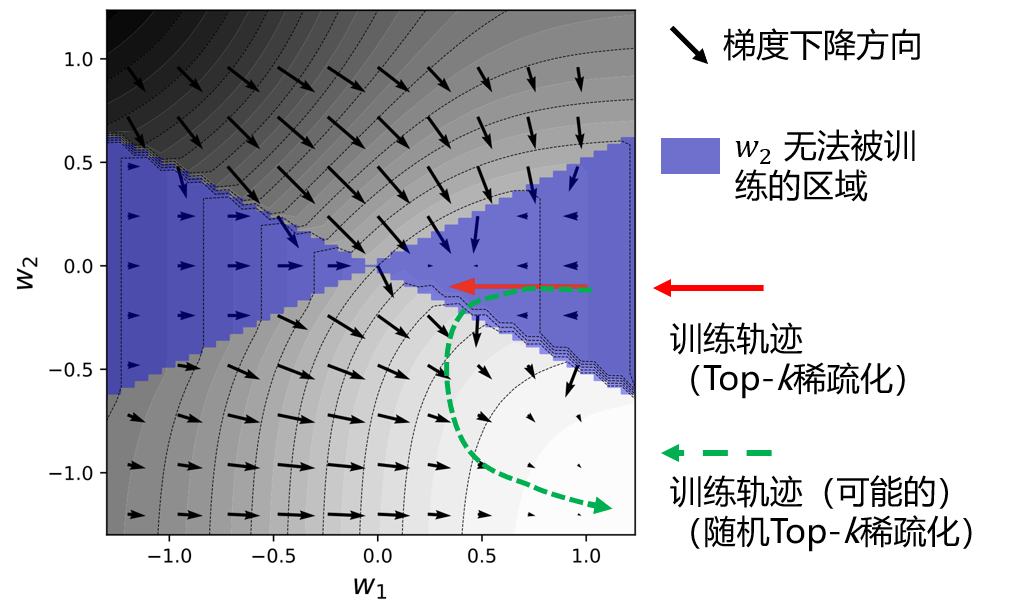
\includegraphics[width=0.75\linewidth]{Z_Resources/randtopk_example.png}
    \caption{使用Top-$k$稀疏化时的损失函数曲面和梯度下降方向}
    \label{fig:randomized_topk:example}
\end{figure}



然而如果在训练过程中使用Top-$k$稀疏化(假设使用平方损失函数),由于$h_2$的值在各个样本上都很小,则$h_2$总是无法被选为Top-$k$,从而导致其对应的权重$w_2$一直无法被训练(对应图中的蓝色区域)。
%
在这种情况下,模型会收敛到一个远离最优点的区域,使得$w_1$降低到$0.4$左右,平衡两个样本的误差,而$w_2$则未被更新而停留在$0.1$处,对应\autoref{fig:randomized_topk:example}中的红色训练轨迹。
%
但是如果在Top-$k$的过程中加入一点随机性,使得$h_2$也有一定的几率被选中,则可以让$w_2$被训练到并且更新,从而摆脱局部最优。
图中的绿色轨迹表明了在Top-$k$稀疏化中加入随机性后产生的一条可能的训练轨迹。


Top-$k$稀疏化的收敛问题也会进一步导致其泛化性能降低。
%
如上文所述,Top-$k$稀疏化带来的泛化优势是因为其表征空间包含了$d \choose k$个超球面,其中$d$是原始的拆分层维度(神经元个数),$k$是稀疏化后保留的维度。
%
但是由于Top-$k$稀疏化带来某些神经元(维度)一直难以得到训练的问题,导致某些神经元在各个样本都无法被选中为Top-$k$,从而导致这些神经元被在模型中无法发挥作用,缩小了表征空间的大小。
%
具体而言,如果采用Top-$k$算法进行训练,假设有$d'$个神经元处于“废弃”状态,则最终得到的表征空间中的超球面数目就会从$d \choose k$减少到$d - d' \choose k$。
%
同样地,如果在Top-$k$稀疏化中加入随机性,将使得各个神经元都有一定的机会被训练,提高表征空间的利用率,从而提高泛化效果。


\subsection{随机Top-$k$算法定义}
基于以上分析,我们可以定义如下的随机Top-$k$算法:
%
选择$k$个要保留的神经元时,每一次选择某个神经元的概率为:
\begin{equation}
\label{eq:randomized_topk:def}
    P(\text{选择该神经元}) = 
    \begin{cases}
        (1 - \alpha) / N_1  & \text{如果该神经元是Top-$k$的,} \\
        \alpha / N_2        & \text{反之.}    
    \end{cases}
\end{equation}
%
其中,$N_1$和$N_2$分别表示当前未被选择的Top-$k$神经元数目和非Top-$k$神经元数目。
%
\autoref{fig:randomized_topk:algo}显示了随机Top-$k$算法的可能执行结果。
%
可以看出,$\alpha$表示选择非Top-$k$神经元的概率。
%
当$\alpha=0$时,随机Top-$k$算法退化为普通的Top-$k$稀疏化;而当$\alpha=1$时,则转变为完全随机的Dropout算法~\cite{srivastava_2014_dropout}。
%
注意到,随机Top-$k$仅仅被应用于模型的训练阶段,在推断阶段,我们依然采用确定性的Top-$k$稀疏化。
%
通过实验,我们发现$\alpha \in [0.05, 0.1]$时模型能取得较好的训练效果。
%
\begin{figure}[h!]
    \centering
    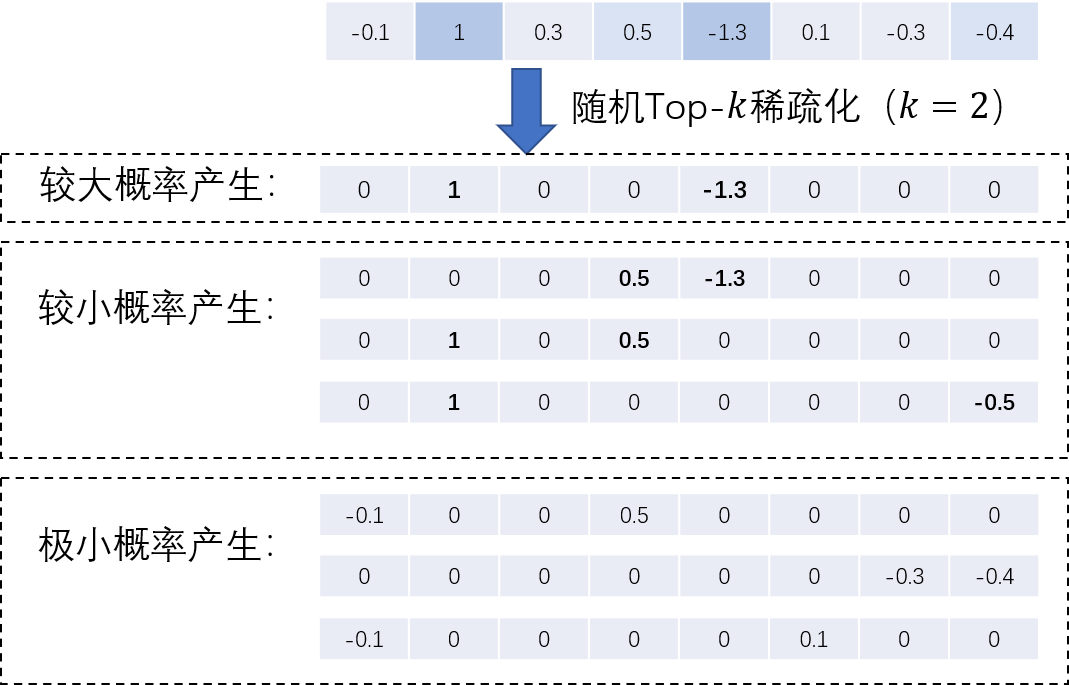
\includegraphics[width=0.7\linewidth]{Z_Resources/randtopk_algorithm.png}
    \caption{随机Top-$k$算法示意图}
    \label{fig:randomized_topk:algo}
\end{figure}


\subsection{隐私分析}
对拆分层表征进行稀疏化后,大部分的拆分层表征元素被丢弃,因此Top-$k$稀疏化或随机Top-$k$稀疏化都能够比原始的拆分学习更多地保护输入特征的隐私。
%
我们在后续实验章节中提供了通过拆分层表征对输入特征进行重建攻击(Reconstruction Attack)的结果。
%
尽管如此,研究表明拆分学习对于标签推理攻击(Label Inference Attack)或模型补全攻击(Model Completion Attack)较为脆弱\cite{fucong2022label_infer_attack},随机Top-$k$算法也并不能解决标签的隐私问题。
%
因此本文考虑的应用场景为标签类别数量大且标签推断攻击不可行的深度学习应用。
%
比如,包含了数千个类别的人脸识别模型、包含了上万种商品的推荐系统模型。
%
对于这些模型,使用者难以获取其他类别对应的输入特征,因此也难以进行标签推断攻击或是模型补全攻击。
%


\section{实验分析}

为了验证本章所提出的随机top-$k$算法的性能,我们在4个不同类型数据集上使用不同的模型进行了实验:
\begin{itemize}
    \item CIFAR-100~\cite{krizhevsky_2009_cifar}: 一个常用的包含了100类总共5万张大小为$32\times 32$的彩色图片。
        我们使用ResNet-20模型~\cite{hekaiming2016resnet}进行分类,拆分层设置为最后的隐层,大小为128。
    %
    \item YooChoose(1/64)~\cite{ben2015yoochoose}:一个推荐系统的数据集,包含了大约15万条用户的点击序列,总共有约1.8万个商品类别。
        我们使用GRU4Rec模型~\cite{jannach2017gru4rec}进行分类,隐层大小设置为300。
        拆分层设置为最后的隐层,大小为300。
    %
    \item DBPedia~\cite{2007dbpedia}:一个文本分类数据集,包含了219种类别,总共有大约34万条文本。
        我们采用TextCNN模型~\cite{kimyoon2014textcnn}进行分类,卷积核的大小为 $(3,4,5)$,并且使用Glove预训练词向量~\cite{pennington2014glove}。
        拆分层设置为最后的隐层,大小为300。
    %
    \item Tiny-Imagenet~\cite{tiny-imagenet}:一个图像分类数据集,包含了200类的10万张彩色图片,图片尺寸为$64\times 64$。
        我们采用EfficientNet-b0模型~\cite{tanmingxing2019efficientnet}进行分类。
        拆分层设置为最后的隐层,大小为1280。
        额外地,我们对权重采用ImageNet的预训练权重和随机初始化两种情况分别进行了实验并汇报结果。
\end{itemize}
%
对于每个任务,我们都测试了不同的模型压缩方法和压缩比率,并且对每一个设定都重复了5次实验取平均值汇报。
%
实验的代码基于Pytorch框架编写,在带有NVIDIA RTX 3090的服务器上进行。
%
实验时我们按照8:1:1的比例划分训练集、验证集合测试集(对于Yoochoose数据集按照先后时间划分),使用Early Stop策略获得验证集上最佳的模型,然后在测试集上进行测试。

\subsection{压缩比率和模型准确率对比}
%
我们测试了模型在测试集上的准确率(对于Yoochoose数据集,我们用前20准确率代替),汇报在。
%
我们把随机top-$k$的随机参数在CIFAR-100, DBPedia, Tiny-Imagenet三个任务上$\alpha$设置为0.1,在Yoochoose任务上设置为0.05。
%
我们把实验结果汇报在\autoref{tab:randomized_topk:main-result}中的。
表内每一项的格式为“准确率/压缩比率*100”,任务名称下方的准确率表示无压缩的普通拆分学习的准确率(压缩比率=100)。
表内空白项表示该方法无法达到对应的压缩比率。
我们用粗体表示同等压缩比率下最高的准确率,用下划线表示次高的准确率。


\begin{table*}[h]
    \centering
    \setlength\tabcolsep{10pt}
    \renewcommand{\arraystretch}{0.8}
    \caption{实验结果:准确率和压缩比率}
    \label{tab:randomized_topk:main-result}
    \small
    \begin{tabular}{@{}ccrrrrr@{}}
    \toprule
    任务          & 压缩  & 随机top-$k$                        & Top-$k$                        & 缩小拆分层             & 量化                 & L1正则化    \\ \midrule
    \multirow{3}{*}{\begin{tabular}[c]{@{}c@{}}CIFAR-100\\      67.20\end{tabular}}\hspace{-3pt}      
        & 高      & \textbf{65.25 / 2.86}       & \underline{62.23 / 2.86} & 55.52 / 3.13       & -                            & -          \\ \cmidrule(lr){2-7} 
        & 中      & \textbf{65.83 / 5.71}       & \underline{61.56 / 5.71} & 60.43 / 6.25       & 53.56 / 6.25          & \underline{62.11 / 8.41}   \\ \cmidrule(lr){2-7} 
        & 低      & \underline{65.98 / 12.4}         & 62.11 / 12.3       & 62.93 / 12.4       & \textbf{66.01 / 12.5} & 63.87 / 19.5          \\ \midrule
    \multirow{3}{*}{\begin{tabular}[c]{@{}c@{}}YooChoose\\      63.57\end{tabular}}\hspace{-3pt}      
        & 高      & \textbf{60.29 / 0.85}       & \underline{60.28 / 0.85} & 50.71 / 1.00       & -                            & -          \\ \cmidrule(lr){2-7} 
        & 中      & \textbf{64.55 / 1.71}       & \underline{63.81 / 1.71} & 62.20 / 2.00       & -                            & -                                   \\ \cmidrule(lr){2-7} 
        & 低      & \textbf{66.88 / 3.84}       & \underline{66.12 / 3.84} & \underline{66.12 / 4.00} & 64.69 / 3.13          & 61.48 / 3.01          \\ \midrule
    \multirow{4}{*}{\begin{tabular}[c]{@{}c@{}}DBPedia\\      93.11\end{tabular}}\hspace{-3pt}        
        & 很高    & \textbf{84.88 / 0.44}       & \underline{83.04 / 0.44} & 64.80 / 0.50       & -                            & -          \\ \cmidrule(lr){2-7} 
        & 高      & \textbf{88.01 / 0.88}       & \underline{85.49 / 0.88} & 78.57 / 1.00       & -                            & 81.35 / 1.08          \\ \cmidrule(lr){2-7} 
        & 中      & \textbf{90.50 / 1.97}       & 87.74 / 1.97       & 86.42 / 2.00       & -                            & \underline{87.88 / 0.93}    \\ \cmidrule(lr){2-7} 
        & 低      & \underline{91.59 / 3.06}          & 90.05 / 3.06       & 88.38 / 3.00       & 91.20 / 6.25          & \textbf{93.11 / 5.31} \\ \midrule
    \multirow{3}{*}{\begin{tabular}[c]{@{}c@{}}Tiny-ImageNet \\ 随机初始化 \\      53.11\end{tabular}}\hspace{-3pt}   
        & 高      & \textbf{50.83 / 0.21}       & 48.36 / 0.21       & 35.46 / 0.23       & -                            & -           \\ \cmidrule(lr){2-7} 
        & 中      & \textbf{51.75 / 0.42}       & \underline{47.24 / 0.42} & 45.66 / 0.47       & -                            &  -                                 \\ \cmidrule(lr){2-7} 
        & 低      & \textbf{51.16 / 0.94}       & 45.50 / 0.94       & \underline{48.87 / 0.14} & -                            & -                                   \\ \midrule
    \multirow{3}{*}{\begin{tabular}[c]{@{}c@{}}Tiny-ImageNet \\ 预训练 \\ 75.18\end{tabular}}\hspace{-3pt} 
        & 高      & \textbf{71.09 / 0.21}       & \underline{70.86 / 0.21} & 59.23 / 0.23       & -                            & -           \\ \cmidrule(lr){2-7} 
        & 中      & \textbf{72.15 / 0.42}       & \underline{71.19 / 0.42} & 66.52 / 0.47       & -                            & -                                   \\ \cmidrule(lr){2-7} 
        & 低      & \textbf{73.83 / 0.94}       & \underline{72.52 / 0.94} & 68.67 / 0.94       & -                            & 67.82 / 1.24          \\ \bottomrule
    \end{tabular}
\end{table*}


实验结果表明,随机top-$k$算法几乎在所有任务上都取得了最好的准确率和最低的压缩比率,且大幅领先于其他方法,在很低的压缩比率情况下依然保持了和原始无压缩拆分学习相近的表现。
%
在YooChoose任务中,随机top-$k$算法甚至超过了无压缩的拆分学习,我们认为这可能归功于随机top-$k$的正则化效果。
%
同时,我们注意到,量化方法和$L1$正则化方法在无法达到一些较低的压缩比率。
这是因为量化方法最低智能达到1/32的压缩比率,并且此时拆分层表征被压缩为2值,往往会导致模型无法收敛。
而$L1$正则化在系数过大时也会导致模型无法收敛。
%

\subsection{训练速度分析}
\begin{figure}[h!]
    \centering
    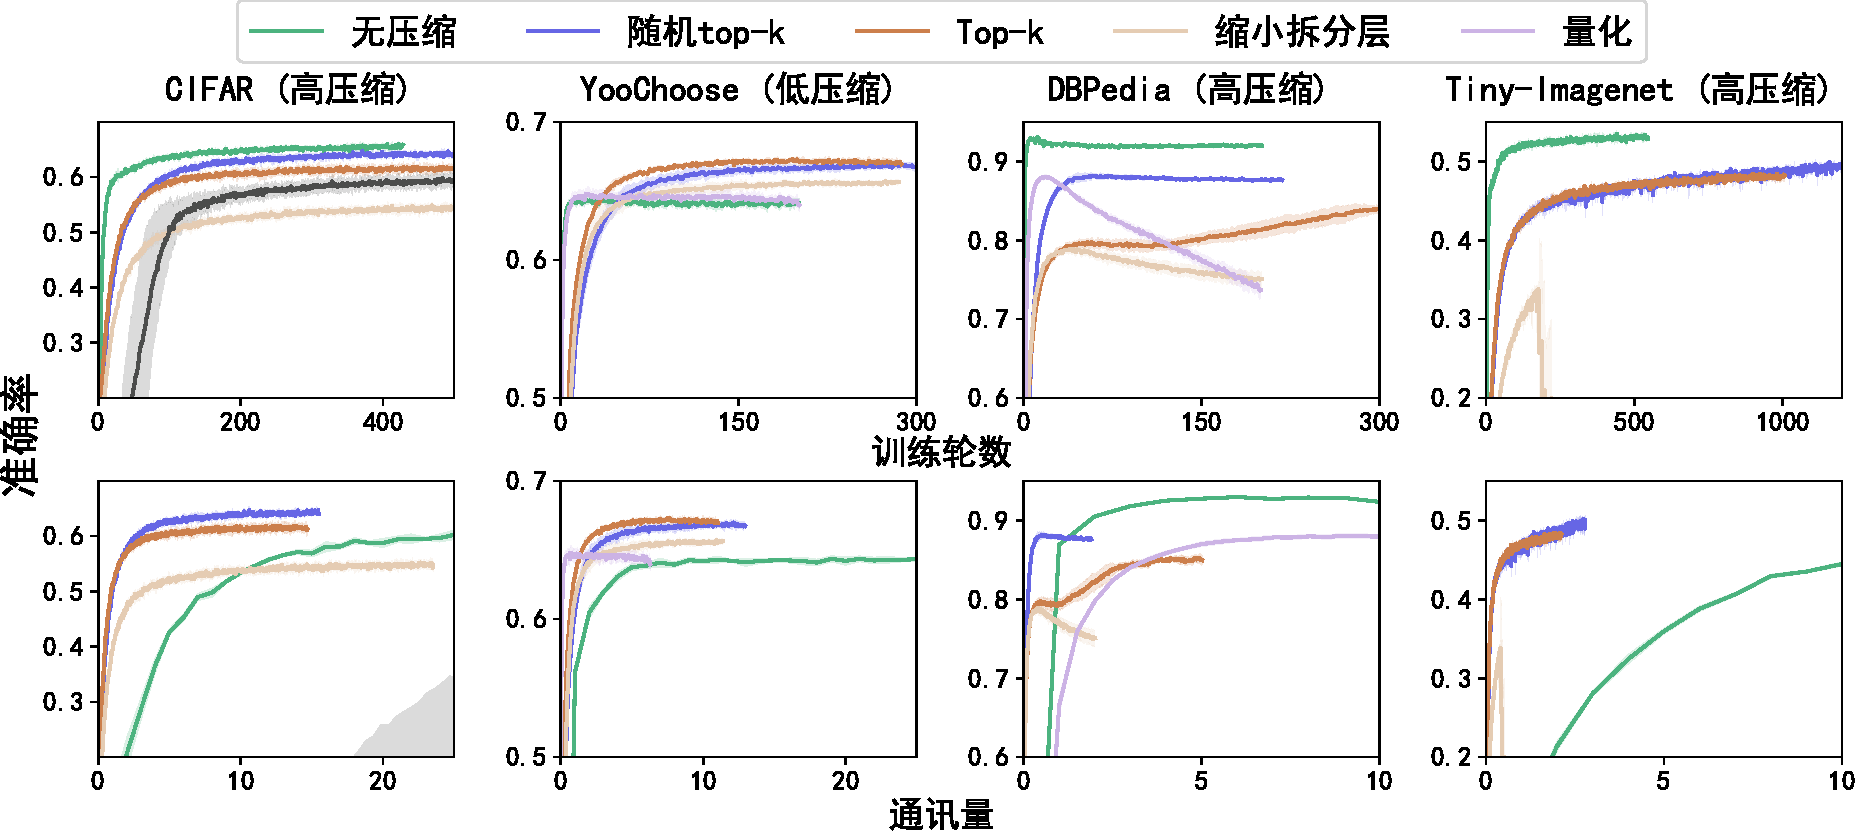
\includegraphics[width=1\linewidth]{Z_Resources/随机topk_训练曲线.pdf}
    \caption{训练轮次/通讯量和准确率}
    \label{fig:randomized_topk:training}
\end{figure}


我们在\autoref*{fig:randomized_topk:training}中汇报了训练过程中准确率和训练轮次以及通信量的关系。
图的第一行是训练轮次和准确率的对比,第二行是通信量和训练轮次的对比,其中我们把一轮无压缩的拆分学习的通信量设为1。
%
实验结果表明,无压缩的拆分学习收敛所需要的训练论次数最少。
但是以通信量衡量时,几乎所有压缩方法的收敛所需的通信量都不无压缩的拆分学习少,并且相比于其他方法,随机top-$k$的收敛速度和准确率都是最高的。
%

\subsection{随机参数$\alpha$分析}
本节我们汇报了变化随机参数$\alpha$时的实验结果,包括了$\alpha$和准确率、收敛速度、泛化误差,top-$k$神经元分布、以及输入特征重构攻击效果的关系,为选取合适的$\alpha$提供参考,并且印证前文关于收敛性、泛化效果以及隐私保护的理论分析。


\begin{figure}[h!]
    \centering
    \begin{subfigure}{0.46\linewidth}
        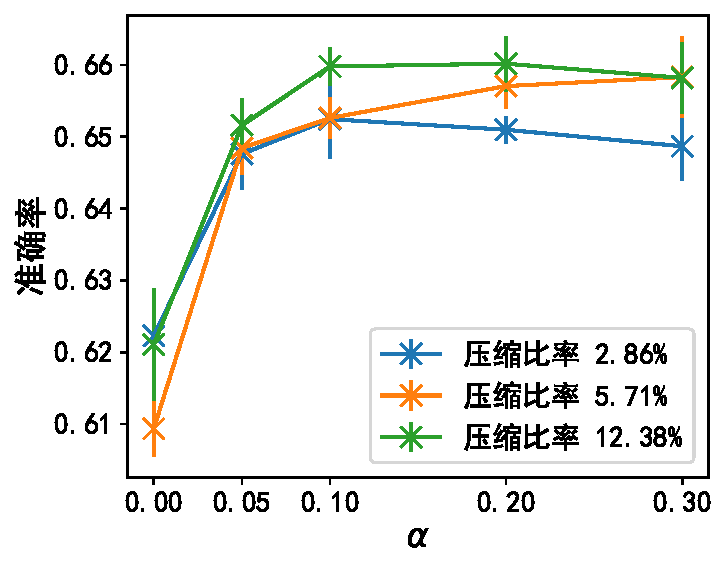
\includegraphics[width=1\linewidth]{Z_Resources/随机topk_cifar-alpha.pdf}
        \subcaption{CIFAR.}
        \label{fig:cifar-trainloss}
    \end{subfigure}
    \begin{subfigure}{0.46\linewidth}
        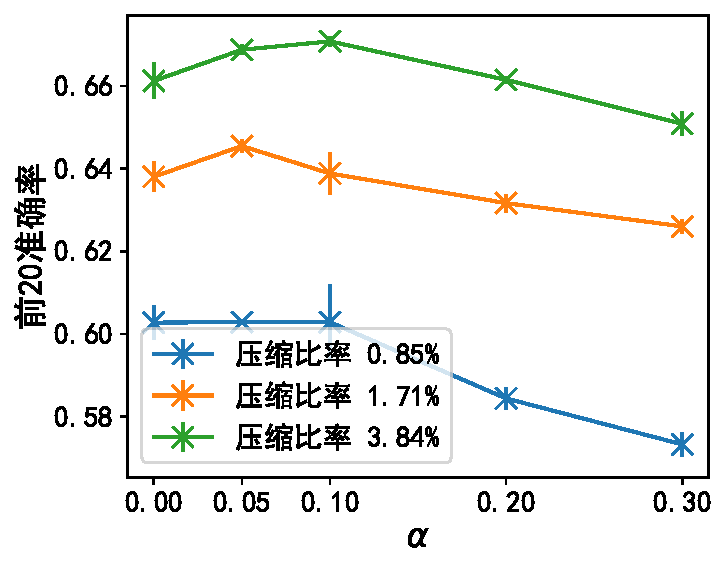
\includegraphics[width=1\linewidth]{Z_Resources/随机topk_yoochoose-alpha.pdf}
        \subcaption{YooChoose.}
        \label{fig:cifar-generror}
    \end{subfigure}
    \caption{$\alpha$与准确率的关系}
    \label{fig:randomized_topk-alpha-acc}
\end{figure}

\textbf{准确率}:
\autoref{fig:randomized_topk-alpha-acc}展示了在CIFAR-100任务中$k=3$情况下,随机参数$\alpha$与模型测试准确率的关系。
可以看出,在CIFAR-100任务中,无论怎样选取$\alpha$都可以比无压缩情况下显著提高准确率,而在YooChoose任务中,提高的幅度则相对有限。
同时,在$\alpha$ 提高到 0.1之后,准确率随着$\alpha$的进一步提高呈现出下降趋势。
%
分析表明,$\alpha \in [0.5, 1]$ 可以使得模型达到较高准确率;而过大的$\alpha$会引入过多的噪声,从而损害模型的效果。


\begin{figure}[h!]
    \centering
    \begin{subfigure}{0.45\linewidth}
        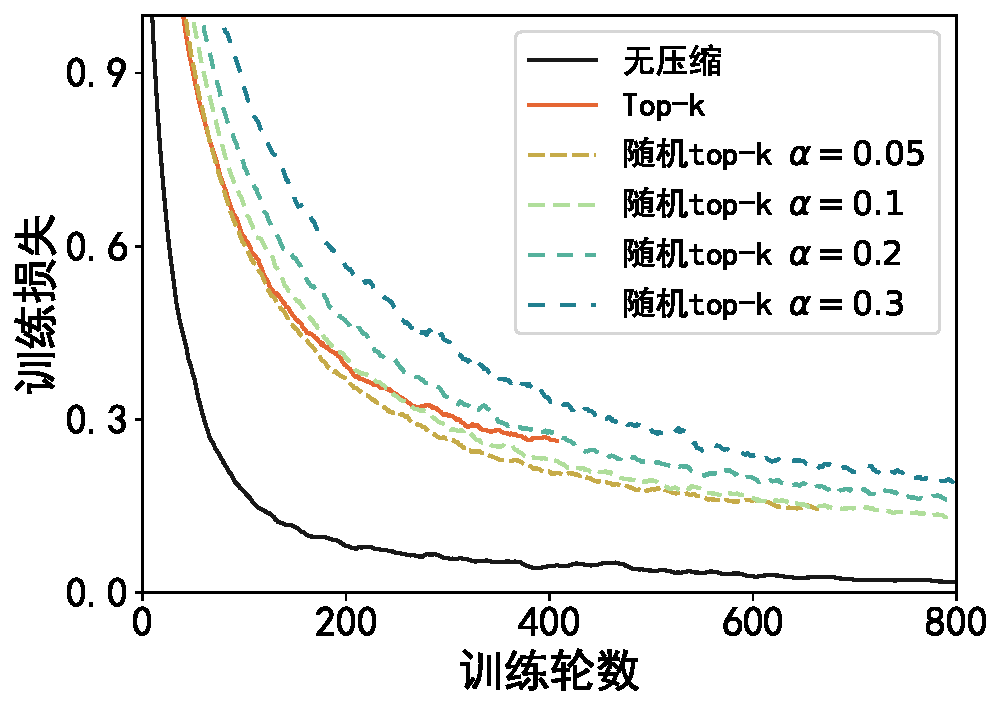
\includegraphics[width=1\linewidth]{Z_Resources/随机topk_cifar100-trainacc.pdf}
        \subcaption{训练损失.}
        \label{fig:randomized_topk-cifar-trainloss}
    \end{subfigure}
    \begin{subfigure}{0.47\linewidth}
        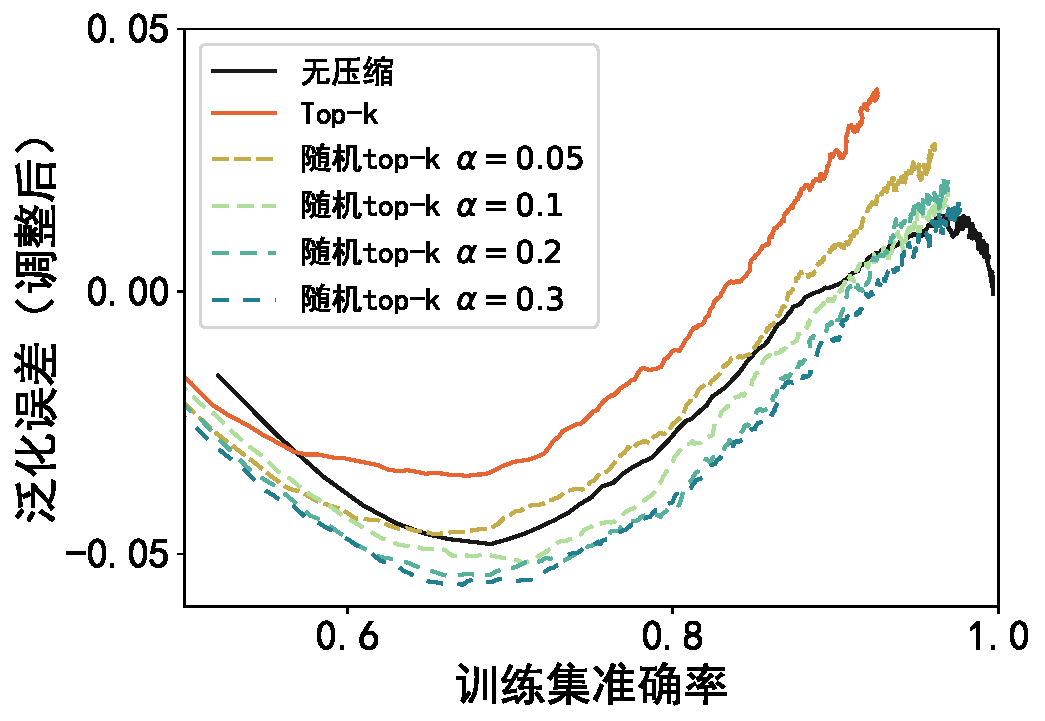
\includegraphics[width=1\linewidth]{Z_Resources/随机topk_cifar100-generror.pdf}
        \subcaption{泛化误差.}
        \label{fig:randomized_topk-cifar-generror}
    \end{subfigure}
    \caption{$\alpha$与训练损失以及泛化误差的关系}
    \label{fig:randomized_topk-alpha-loss}
\end{figure}
\textbf{收敛性和泛化误差}:
\autoref{fig:randomized_topk-alpha-loss}展示了在CIFAR-100任务中$k=3$情况下,随机参数$\alpha$与模型训练损失和泛化误差的关系。
为了更清晰呈现泛化误差的变化,我们再对泛化误差进行了调整,将\autoref{fig:randomized_topk-cifar-trainloss}调整为的Y轴调整为如下:
\begin{equation}
    y = \text{泛化误差(训练集准确率 - 测试集准确率)} - 0.5 \times \text{训练集准确率} + 0.2.
\end{equation}
%
从图中可以看出,top-$k$稀疏化在训练开始时损失下降较快,但是随着训练轮数的增长,随机top-$k$的损失下降变快,并且最终收敛的损失低于top-$k$。
另外,太大的$\alpha$也导致损失下降变慢。
%
同时,相对于无压缩的情况,top-$k$稀疏化显著增加了泛化误差。而增大$\alpha$也显著降低了泛化误差。
%
这和我们在\autoref{sec:randomized_topk:method}中对于随机top-$k$算法的收敛性和泛化性的理论分析相对应。



\begin{figure}[h!]
    \centering
    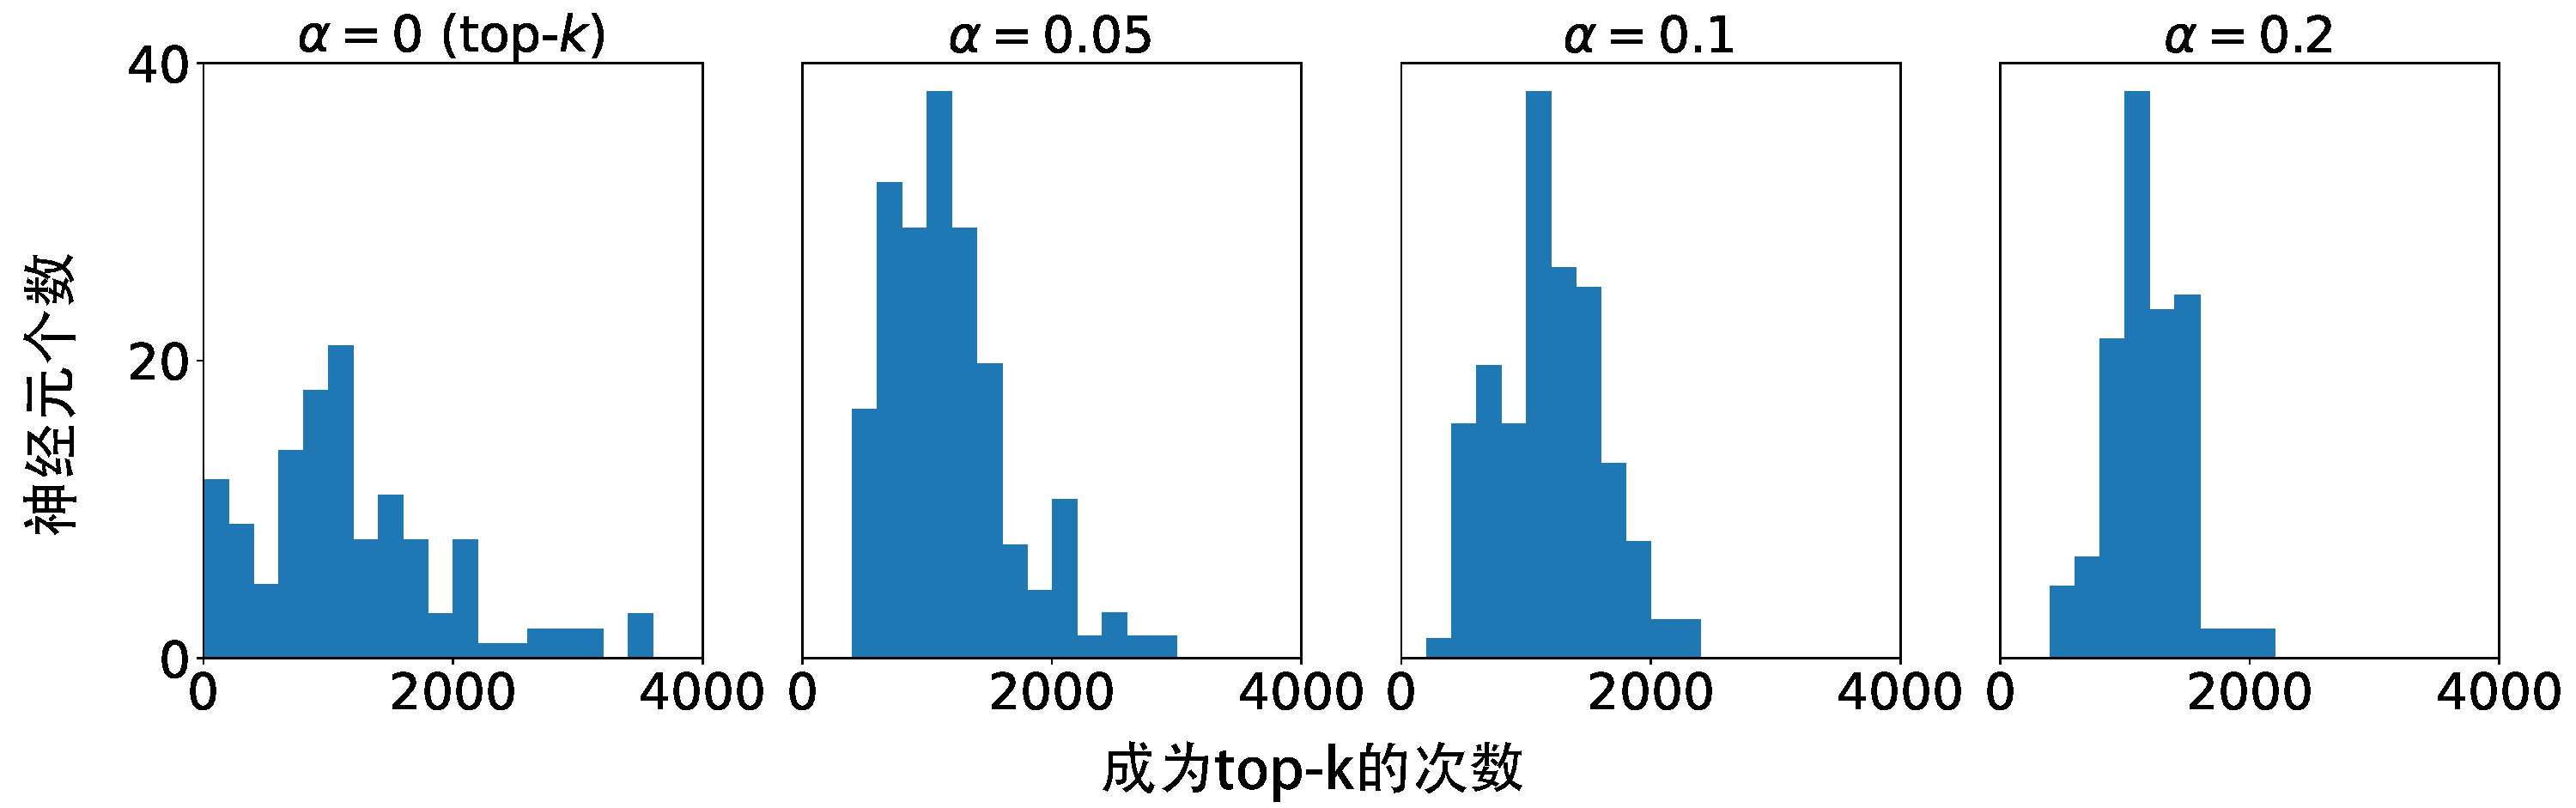
\includegraphics[width=\linewidth]{Z_Resources/随机topk_cifar100-dist-topk.pdf}
    \caption{两方拆分学习推断示意图}
    \label{fig:randomized_topk-dist}
\end{figure}

\textbf{Top-$k$神经元的分布}
\autoref{fig:randomized_topk-dist}显示了采用不同的$\alpha$训练后,在推断阶段使用测试集样本时,神经元被选为top-$k$次数的分布。具体而言,隐层的第$i$个神经元被选为top-$k$的次数按照如下公式计算:
\begin{equation}
    C_i = \sum_{j=1}^N [\text{$M_b(X_j)$的 top-$k$ 神经元包含了其第 $i$ 个神经元(是=1,否=0)}],
\end{equation}
其中,$N$表示测试集样本数,$X_j$表示第$j$个样本。
%
%
可以看出,仅使用top-$k$稀疏化时,神经元被选为top-$k$次数的分布不均匀,部分神经元几乎从未被选为top-$k$,而某些神经元则总是被选中;而使用随机top-$k$有效地解决了这一问题,top-$k$次数的分布变得均匀,说明各个神经元被选为top-$k$的概率更加均等。
%
即使是一个较小的$\alpha$(0.05),也能显著使得top-$k$次数的分布变得均匀。
%
这也说明,随机top-$k$更好地利用了表征空间,从而提高了泛化性能。
%


\begin{figure}[htbp]
    \centering
    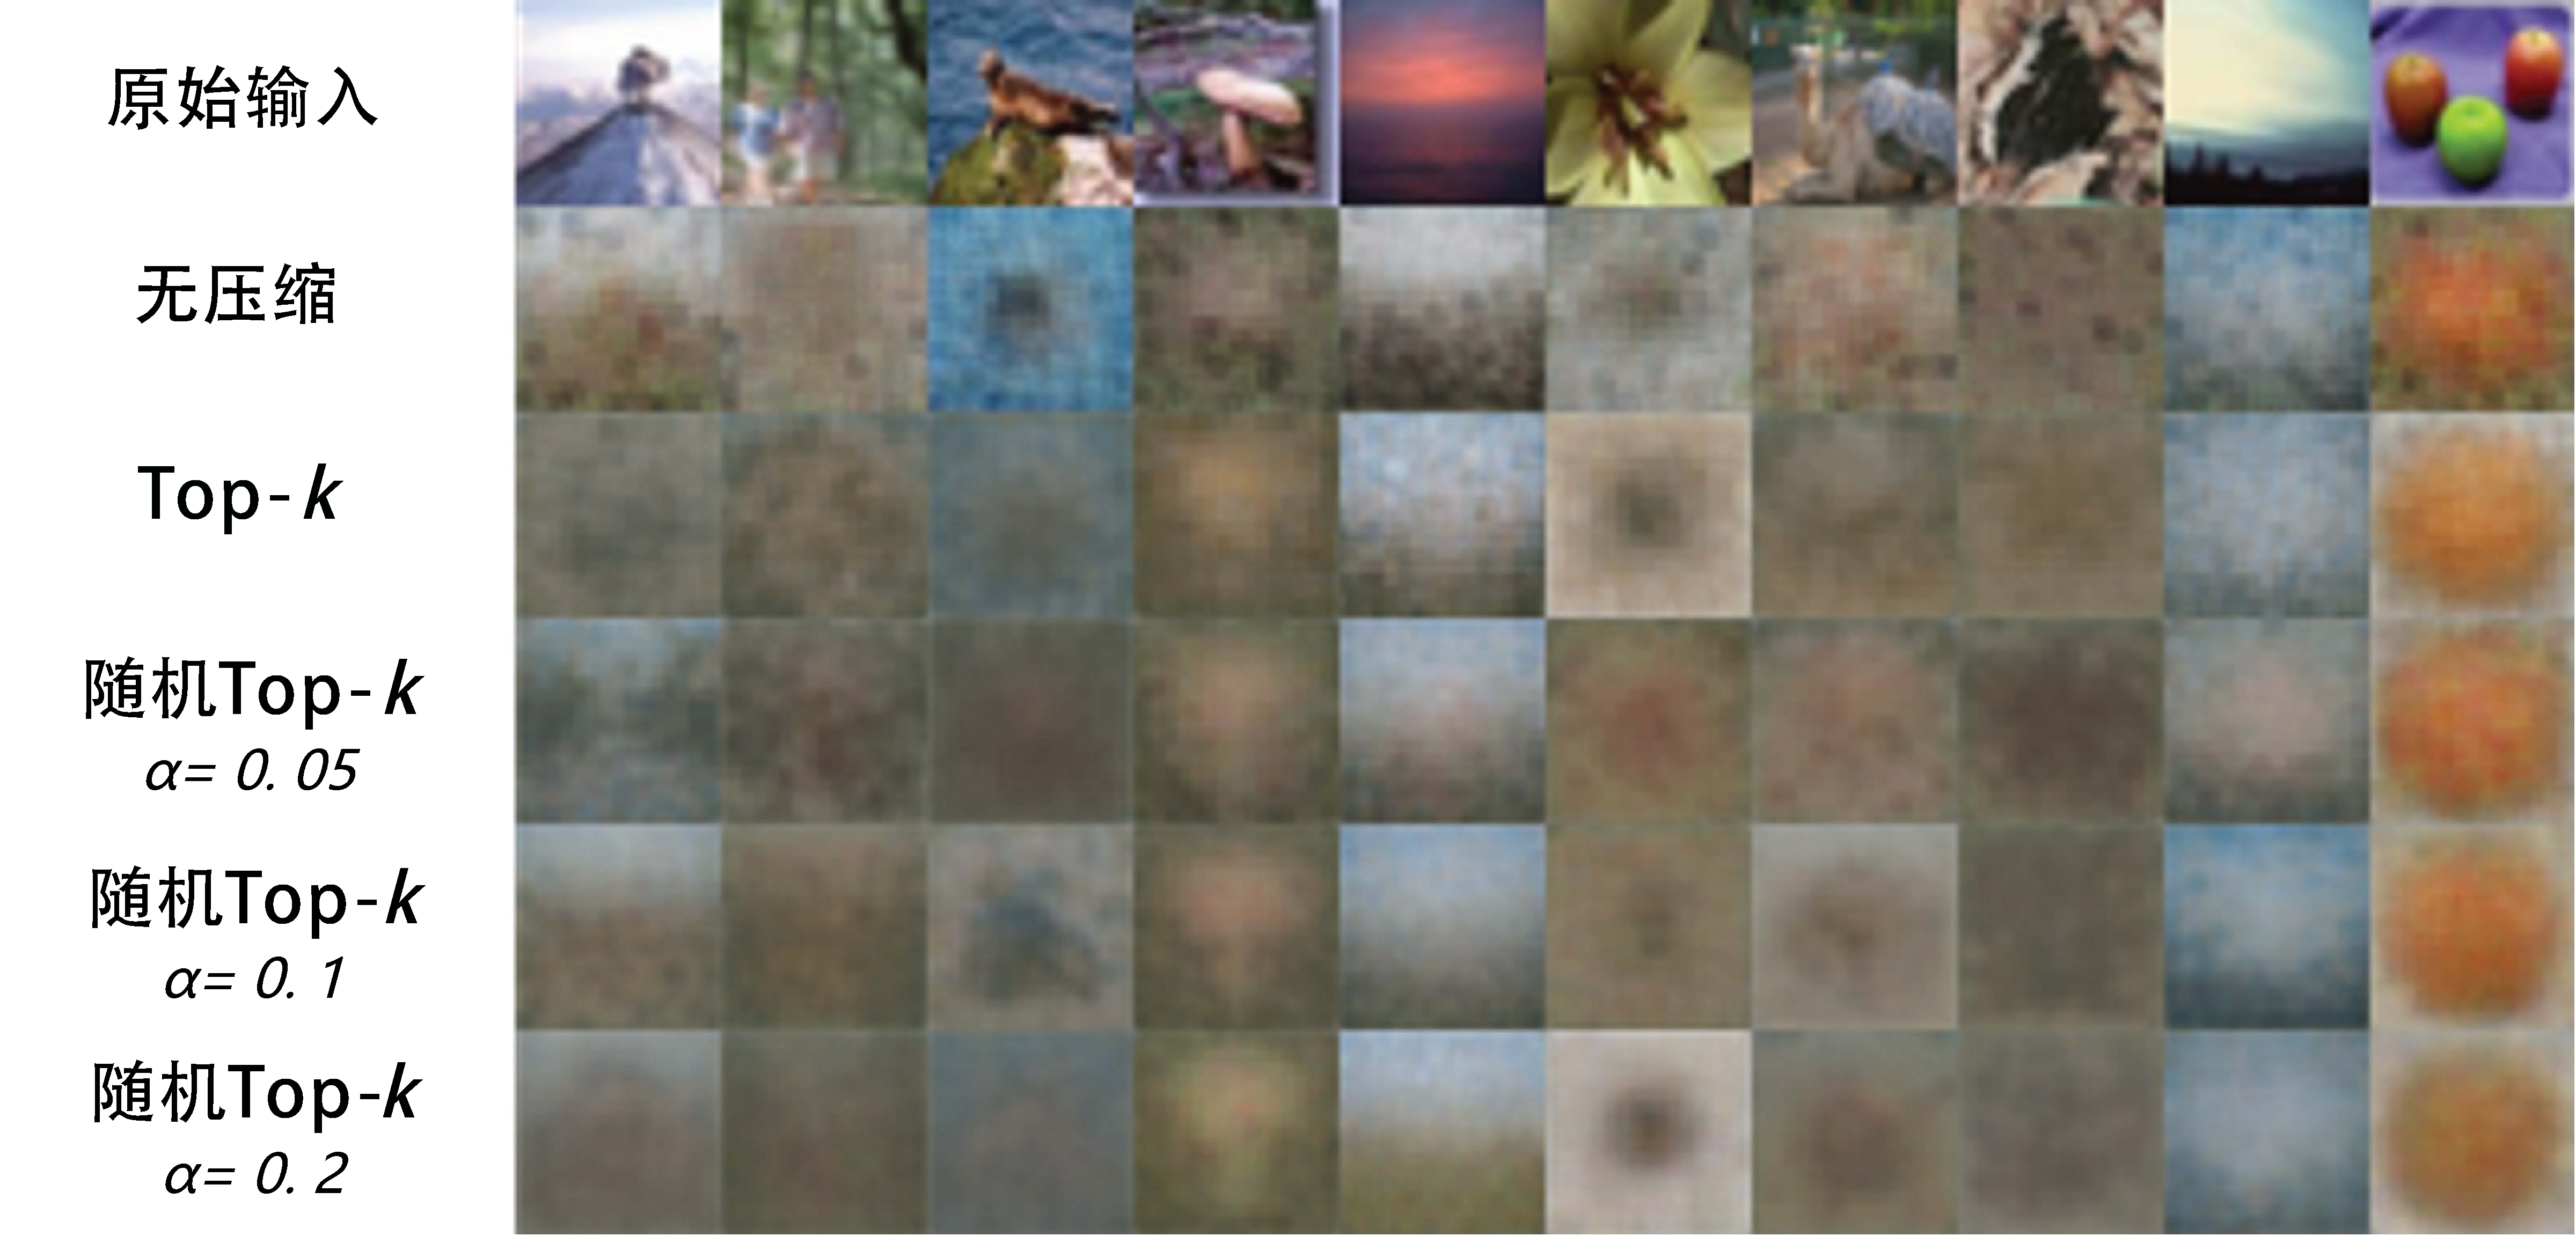
\includegraphics[width=\linewidth]{Z_Resources/随机topk_inversion-attack.pdf}
    \caption{CIFAR-100输入重建攻击效果}
    \label{fig:randomized_topk-inversion_attack}
\end{figure}

\begin{figure}[h!]
    \centering
    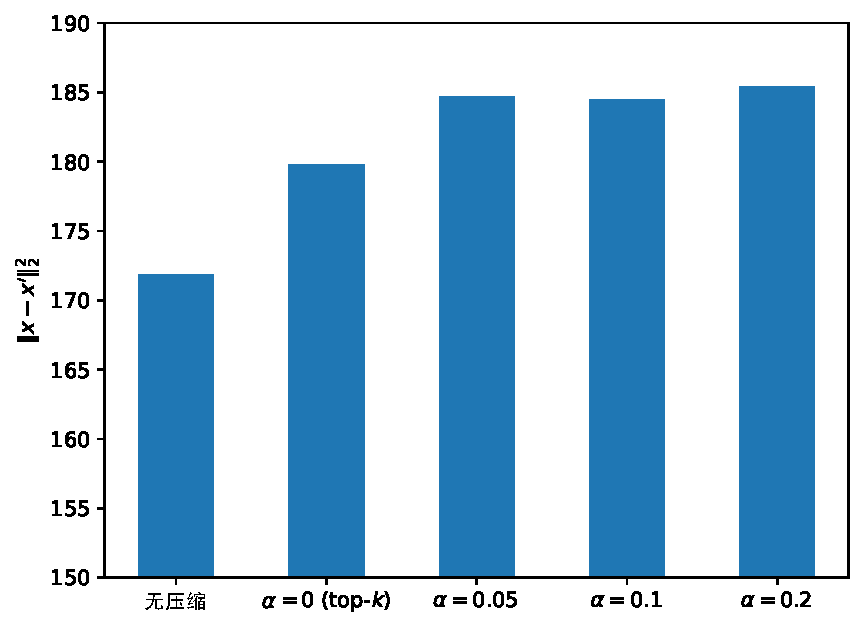
\includegraphics[width=0.58\linewidth]{Z_Resources/随机topk_attack-error.pdf}
    \caption{CIFAR-100输入重建攻击误差}
    \label{fig:randomized_topk-attack-error}
\end{figure}


\subsection{隐私分析}
为了表明随机top-$k$压缩方法对于输入数据的隐私的影响,我们在CIFAR-100数据集上进行了输入特征重建攻击的实验。
%
输入重建攻击是一种从隐层恢复出输入数据的手段,其方法是通过泄漏的数据,训练一个重构神经网络将拆分层数据逆向回原始输入特征~\cite{hezecheng_2019_model_inversion_attack,vepakomma2020nopeek}。
%
本实验中,重构神经网络的结构为(全连接,卷积,反卷积,卷积),其中全连接层将128维拆分层投影为$4 \times 16\times 16$ (4表示频道数),此后三层的输出大小分别为$16\times 16 \times  16$,$32\times 32 \times 32$,$3\times 32 \times 32$。激活函数为LeakyReLU~\cite{maas2013leaky_relu}。

\autoref{fig:randomized_topk-inversion_attack}展示了在CIFAR-100任务中$k=3$情况下,在模型推断阶段,攻击者根据拆分层表征对原始输入图片进行恢复攻击的效果。
从图中可以看出,由于拆分层被设置在最后一层线性层,因此即使是无压缩的情况下,攻击者依然难以还原图片的主要信息,只能呈现出模糊的类似于类别的“平均图”的图片。
%
而top-$k$和随机top-$k$进一步使得原始图片中的色彩信息几乎也被丢失。
%

为了更加清晰地现实随机top-$k$和其他方法的输入特征隐私保护效果,我们测量了图片恢复攻击的平方误差,即$\mathbb E\left[ \Vert \text{恢复值} - \text{原始值} \Vert_2^2 \right]$,并汇报在\autoref{fig:randomized_topk-attack-error}中。
%
从图中可以看出,top-$k$稀疏相对于原始无压缩的拆分学习显著提高了攻击者的重建损失,增强了隐私保护效果。
而随机top-$k$比top-$k$拥有更高的重建损失,说明其进一步提高了对于输入特征的隐私保护。



\section{本章小结}
本章节针对多分类拆分学习中的通信效率问题,提出了随机Top-$k$稀疏方法,并且从泛化误差、收敛性以及隐私性三个角度进行了理论和实验分析,证明了随机Top-$k$算法的优越性。
%
我们通过近似计算表征空间大小,表明了Top-$k$算法在同等压缩率下拥有更大的表征空间,从而使各个类别的决策区域更大,带来更低的泛化误差。
%
同时,通过一个二维例子说明了Top-$k$算法在收敛性上可能面临部分神经元无法被训练到的问题,而在Top-$k$中加入随机性可以有效地防止该类问题。
%
基于以上分析,我们提出随机Top-$k$算法对传统的Top-$k$进行了改进。
%
通过与Top-$k$算法、拆分层量化、L1正则化、缩小拆分层等方法对比,随机Top-$k$显示出了其在拆分学习训练与推断过程中的优越性,包含了更高的模型准确率和训练/推断速度。
%
此外,实验结果也表明稀疏化后的拆分层表征也能降低对于输入特征的隐私泄漏问题。
%
总之,随机Top-$k$算法显著提高了类别数量众多时拆分学习训练和推断过程中的通信效率,为拆分学习模型在实际应用中的部署提供了有力支持。

    \chapter{基于势能损失的隐私保护拆分学习}
\section{研究背景}
拆分学习是一种高效的隐私保护机器学习手段~\cite{vepakomma2018split,poirot2019split}。
在拆分学习中,模型被分割为数个部分分发给各个参与方,各个参与方在模型的训练或推断过程中只需要交换中间结果而非原始数据,在一定程度上保护了数据的和模型参数的隐私。
%
相比于基于密码学的隐私保护机器学习方法,拆分学习具有非常高的通讯和计算效率。
%
如今拆分学习已经被应用在机器学习的多个领域中~\cite{palanisamy2021spliteasy,fagbohungbe2022split_edge_image,ccc2022vfgnn}。

由于第\ref{chap:randomized_topk}章中已经对拆分学习进行了基本的介绍,本节对此不再赘述。
%
虽然拆分学习拥有实现简单、效率高等诸多优势,但是在训练和推断过程中,各方直接交换了中间结果和中间梯度的明文,从而存在一定的隐私泄漏风险。
%
本章主要考虑的是拆分学习中的模型和标签数据的隐私问题。
%
不失一般性地,我们考虑两方拆分学习的场景,其中用户拥有输入特征($X$),而模型拥有方拥有模型参数并把底部模型($M_b$)下发给用户。
一个两方拆分学习推断的流程可以表示为:
\begin{equation}
    X \stackrel{M_b}{\to} H \stackrel{M_t}{\to} Y,
\end{equation}
其中,$X$是输入特征,$H$是拆分层的隐层表征,$Y$是预测的样本标签,而$M_b, M_t$表示底部模型和顶部模型。
%
可以看出,拆分层表征$H$同输入特征$X$、预测值$Y$都具有一定的相关性,因此有一定的隐私泄露风险。


目前已经有一些研究考察了从拆分层表征逆推输入特征的攻击,并提出了对应的防御手段,如Vepakomma等人~\cite{vepakomma2020nopeek}提出了在训练过程中加入额外的基于距离相关性~\cite{szekely2007dcor}的损失函数$\text{Dcor}(H, X)$来减少表征中包含的输入信息,并取得了一定的效果。
%
而拆分层表征泄露标签隐私的问题则更为严重。
%
Fu等人~\cite{fucong2022label_infer_attack}提出通过少量泄漏的带标签样本即可从随机初始化训练出顶部模型,从而窃取样本的标签以及整体模型,并将这种攻击称之为模型补全攻击(Model Completion Attack)。
%
针对这种攻击,Sun等人~\cite{sunjiankai2022forward_embedding_protect}提出使用距离相关性对表征和输出标签进行解耦,并取得了一定的效果。
%
除此之外,拆分学习的训练过程中的梯度也会泄露标签隐私。
Li等人~\cite{oscarli2022label_defense_marvell}表明的拆分层的梯度和样本标签的相关性很高,并提出了一些对于二分类模型的防御方法。
Sanjay等人~\cite{sanjay2023exploit_split_learning}在训练时采用替代的头部模型对梯度进行匹配从而实现盗取标签的目的。
%
本文研究的是针对分类模型的拆分学习推断阶段,尽可能地对$H\to Y$这一隐私泄漏链条进行保护,防止模型补全攻击。

直觉而言,拆分层表征泄露模型输出信息似乎是不可避免的。
%
因为在模型训练过程中,其逐渐丢弃隐层表征中关于输入特征的无关信息,只保留与标签相关的信息。
为了模型能产生准确的预测,隐层表征中必须包含关于标签的信息。
%
因此,本文并不尝试将标签相关信息从拆分层表征中彻底删除,而是把攻击问题转化成一个监督学习或无监督学习问题,研究如何使得攻击者难以从拆分层表征中获取标签信息。
%

\section{问题描述}
本节我们对拆分学习中底部模型产生的拆分层表征带来的对顶部模型以及标签的隐私泄漏问题(模型补全攻击)进行描述和定义,并且将该隐私泄漏问题转化为一个攻击者的有监督或无监督的学习问题。

\begin{figure}[h!]
    \centering
    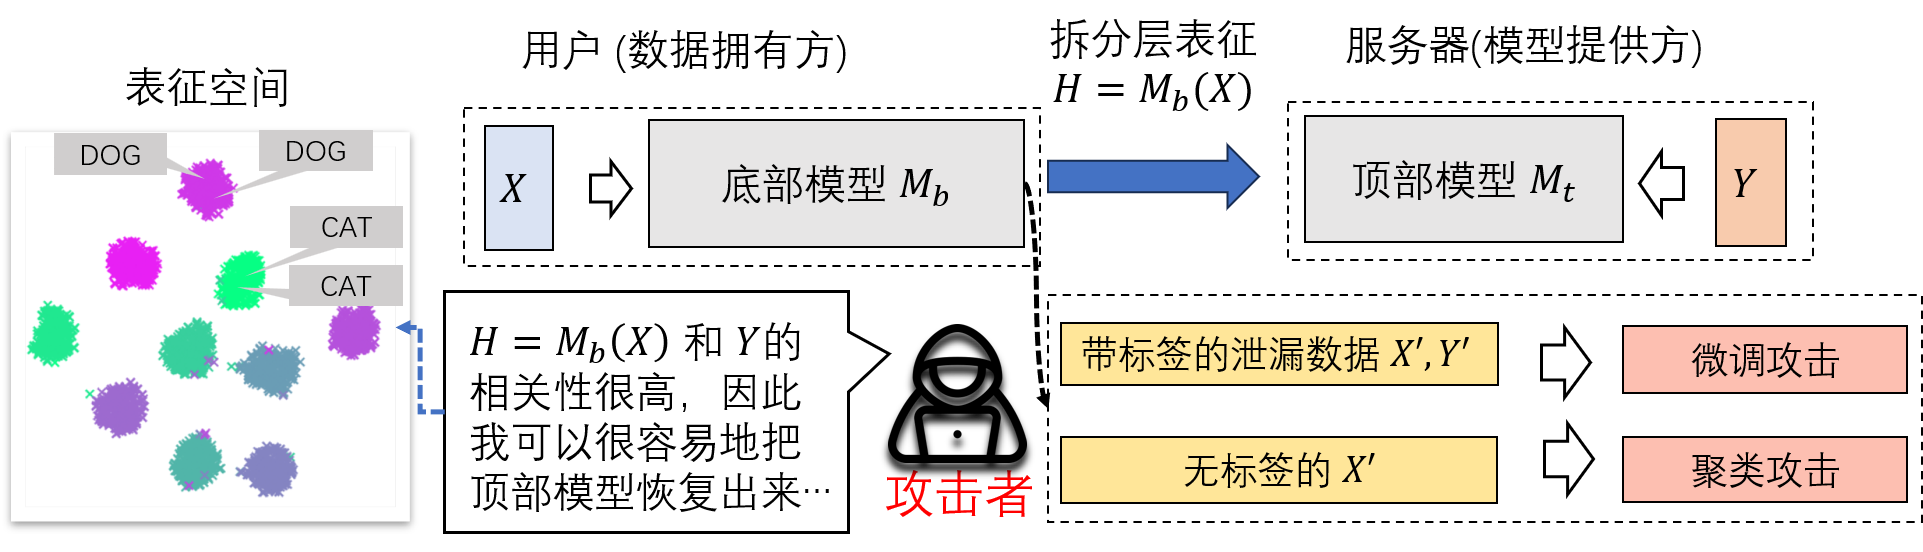
\includegraphics[width=1\linewidth]{Z_Resources/peloss_attack.png}
    \caption{拆分学习中底部模型带来的隐私泄露问题和模型补全攻击示意图}
    \label{fig:peloss:attack}
\end{figure}

\subsection{拆分层的隐私泄露}
许多对神经网络隐层进行可视化的研究都揭露了如下的规律:在神经网络的训练过程中,隐层表征与样本标签的关联性逐渐增加,相同标签对应的隐层表征会逐渐聚集成簇,而不同标签对应的隐层表征会逐渐分离开~\cite{paulo2017visualize_hidden,pezzotti2017deepeyes,cantareira2020hidden_vector_fields}。
%
并且位置越靠后(接近模型输出)的隐层的表征,与样本标签的关联性越高。
%
尽管上述的“同类别隐层表征靠近,不同类别隐层表征分离”的规律是神经网络具备学习能力的一个重要原因,这个规律也给拆分学习带来了很大的隐私泄漏风险。
%

理想的两方拆分学习$X \stackrel{M_b}{\to} H \stackrel{M_t}{\to} Y$应该满足下述的两个条件:
\begin{itemize}
    \item 从$H$推出$X$是困难的,从而保证用户的输入数据的隐私。
    \item 从$H$推出$Y$是困难的,因此用户必须和模型拥有方合作,才能获取模型预测值,而不能仅仅通过$M_b$获取预测值,从而保证模型的隐私。
\end{itemize}
然而,前面所述的神经网络隐层表征的性质,恰恰说明$H$推出$Y$可能是十分容易的,与我们期望的理想拆分学习的性质所矛盾。
%
假设攻击者腐化了用户,它可以轻松地通过少量带标签样本$(\cdots, (X_i, Y_i), \cdots)$,然后通过用户侧的底部模型$M_b$来产生拆分层表征$(\cdots, H_i, \cdots)$,并通过拆分层表征-标签对$(\cdots, (H_i, Y_i), \cdots)$来训练顶部模型$M_t$,从而窃取整个模型;
同时,攻击者也可以直接通过无标签的样本产生大量表征,并对其进行聚类得到类别标签,从而得到样本标签$Y$或训练出顶部模型$M_t$。
%
我们将这两种攻击统称为模型补全攻击,与现有研究一致~\cite{fucong2022label_infer_attack,liu2024vertical}。
%
\autoref{fig:peloss:attack}是模型补全攻击的示意图。


\subsection{威胁模型}
为了更清晰地定义上述的隐私泄漏问题,我们定义两种攻击方法:
\begin{itemize}
    \item \textbf{微调攻击}:
    假设攻击者具有底部模型$M_b$,并且拥有少部分泄露的带标签样本$Z = (\cdots, (X'_i, Y'_i), \cdots)$,其中每一种类别的样本都有$k$个。攻击者也知道顶部模型$M_t$的结构,但是不知道具体参数。
    攻击者通过泄漏样本$Z$和固定的$M_b$来微调(Fine-Tune)$M_t$,从而实现窃取模型的目的。

    \item \textbf{聚类攻击}:
    假设攻击者具有底部模型$M_b$,并且拥有大量泄漏的无标签样本$X = (\cdots, X_i, \cdots)$。
    攻击者通过$M_b$产生中间表征$H = (\cdots, H_i = M_b(X_i), \cdots)$,然后对其进行聚类产生类别标签,使得聚类模型实现顶部模型$M_t$的功能,从而窃取整个模型。
\end{itemize}

注意到,我们的攻击场景设定为拆分学习的推断阶段而非训练阶段,因为本文的目标是降低拆分层表征的隐私泄露。
%
如果要对拆分层梯度进行保护,可以使用非敏感数据进行训练,或者使用基于密码学的隐私保护神经网络训练方法~\cite{mohassel2017secureml,wagh2019securenn}。
%
除此之外,一些研究也指出对于无标签的样本进行无监督学习也能产生一个表现良好的分类模型~\cite{berthelot2019mixmatch,xuyi2021dp_ssl}。
但是这些方法与拆分学习无关,因为它们不需要任何关于底部模型或是拆分层表征的知识。
因此本文不考虑这些方法。
%

\subsection{问题定义}
表面上看来,上述的攻击和模型正常的训练过程的目标是类似的:两者都会学习从拆分层表征$H$到标签$Y$的映射。
%
然而攻击者的训练过程和正常的模型训练过程存在着一个本质区别,即两者的训练数据不同。
正常的模型训练过程需要大量的带标签数据,而在模型补全攻击中,我们假设攻击者只能获取少量的带标签样本(或是一定数量的无标签样本)。
%
因此,我们可以把模型补全攻击转化成一个机器学习问题,即攻击者使用少量带标签样本以及训练好的底部模型$M_b$来学习顶部模型$M_t$。
具体而言,防御的目标转换为:控制底部模型$M_b$,使得整体模型$(M_b, M_t)$有较高的准确率,但是使用少量带标签的$H = M_b(X)$对随机初始化的$M_t$进行微调,则会产生较高的泛化误差。
%

\begin{definition}[底部模型优势]
    我们定义底部模型优势为攻击者利用底部模型$M_b$进行攻击产生的额外优势。
    考虑一个攻击者$\mathcal A$和其输入数据$D$以及底部模型$M_b$(可以为空),其输出则为一个完整模型$M = (M_b, M_t): X \to Y$,底部模型优势可以定义为:
    \begin{equation}
        Adv(M_b; \mathcal A) = \mathbb E_D \{ R[\mathcal A(D; null)] - R[\mathcal A(D; M_b)]\},
    \end{equation}
    其中,$R[\cdot]$ 表示攻击者产生的完整模型在测试集上的误差,$\mathcal A(D; null)$ 表示攻击者在没有底部模型时的产生的完整模型。
\end{definition}
%
例如,在微调攻击时,$D = (\cdots, (X_i, Y_i), \cdots)$ 是泄露的带标签的样本;而在聚类攻击时,$D = (\cdots, X_i, \cdots)$是泄露的无标签的样本。
%
而$\mathcal A(D; null)$相当于攻击者在没有任何底部模型信息,仅有泄露数据的情况下产生的完整模型,即使用带标签数据/无标签数据从零开始训练模型(Train from Scratch)。

\begin{definition}[完美保护]
    对于某种攻击$\mathcal A$,如果底部模型$M_b$满足底部模型优势$Adv(M_b, \mathcal A) \le 0$,则称$M_b$对$\mathcal A$产生了完美保护,因为$M_b$的存在对攻击效果的提升没有任何作用。
\end{definition}

基于以上定义,本文目标可以描述为训练一个拆分学习模型$(M_b, M_t)$使得:
\begin{itemize}
    \item 模型本身的准确率越高越好。
    \item 微调攻击和聚类攻击的底部模型优势越小越好。
\end{itemize}
\section{势能损失函数}
如上节所述,我们把模型补全攻击考虑为攻击者基于泄露数据的机器学习过程。
%
本节我们研究攻击者在泄露样本上学习得到的顶部模型的泛化误差。
我们通过二分类例子表明当拆分层表征分布在决策边界附近时,攻击者的泛化误差较大。
%
受到静电平衡理论以及库仑定律的启发,我们提出了势能损失,使得拆分层表征满足上述的分布,从而实现对于模型补全攻击的保护。
%

\subsection{数据分布导致的学习误差}
我们从微调攻击的泛化误差以及聚类误差两个角度来说明同类样本分布在决策边界附近时可以使得攻击者的学习误差变大。


\subsubsection{泛化误差}
直观地说,当同类表征分布在决策边界附近时,表明同类表征之间的距离加大,从而使得少量该类别的表征无法代表整个类别的表征,因此会提高攻击者在少量样本上训练顶部模型的泛化误差。
%
下面我们使用一个二分类的例子对其进行说明。
%

考虑表征空间为一个$d$维超球体($d$-sphere)$\{ \bvec{x}: \sum_{i=1}^d x_i^2 = 1\}$,所有表征被划分为两个类别(正样本和负样本)。
令假设集(Hypothesis Set,即所有可能的分类函数的集合)为所有的半球面(表示正样本)集合:
\begin{equation}
    \mathcal H = \{ h: h(\bvec{x}) = \text{Sign}(\bvec{w} \cdot \bvec{x}), \Vert \bvec{w} \Vert_2 = 1\}.
\end{equation}
不失一般性,我们假设目标分类函数为$f(\bvec{x}) = \text{Sign}(x_1)$。
同时,我们对表征的分布做出如下假设:
\begin{itemize}
    \item 表征分布的概率密度仅仅和其坐标的第一维有关,也就是仅和$x_1$有关,而在其他维度上呈现出各向同性(Isotropic)性质。
    \item 给定一批正样本数据$S = \{\bvec{x}_1, \cdots, \bvec{x}_n\}$,学习算法简单地产生其归一化(Normalized)的平均值作为学到的分类模型的权重$\bvec{w}$。
    即:
    \begin{equation}
        f^{(S)}(\bvec{x}) = \text{Sign}\left[ \bvec{x} \cdot \sum_{i=1}^n {\bvec{x}_i} / \Vert \sum_{i=1}^n {\bvec{x}_i}\Vert_2 \right].
    \end{equation}
\end{itemize}

考虑当学习到的参数$\bvec{w} = \sum_{i=1}^n \bvec{x}_i / \Vert \sum_{i=1}^n \bvec{x}_i \Vert_2$ 与目标分类模型的参数 $\bvec{e}_1$ 有一个很小的偏差时的情况。
%
由于我们假设表征的分布在$\bvec{e}_1$之外的维度时各向同性的,我们可以假设$\bvec{w}$位于前两维展开的超平面上,也就是
\begin{equation}
    \bvec{w} = \bvec{e}_1 \cos \epsilon + \bvec{e}_2 \sin \epsilon,    
\end{equation}
其中$\epsilon$表示$\bvec{w}$和$\bvec{e}_1$之间的一个小角度。
%
此时我们可以得到泛化误差为:
\begin{equation}
\begin{split}
    1/2\cdot R[\bvec{w}] &= \mathop{\mathbb E}_{\bvec{x} \sim \mathcal S} \text{Sign}(x_1) \cdot I[x_1 \cos \epsilon + x_2 \sin \epsilon \le 0]
    \\
    & = \int_{\substack{x_1 > 0 \\ x_1 \cos \epsilon + x_2 \sin \epsilon \le 0 \\ x_1^2 + \cdots + x_d^2 = 1}} p(x_1, \cdots, x_d)dS
      \le \int_{\substack{x_1^2 + ... + x_d^2 = 1 \\0 < x_1 \le \tan\epsilon}}p(x_1, x_2, ...,x_d)dS
\end{split}
\end{equation}
注意到当$\epsilon \to 0$时,$\tan \epsilon \to \epsilon$,并且令$p_1$为表征在$\bvec{e}_1$上的边缘概率密度,即$p_1(x_1) = \int_{x_1^2 + \cdots + x_d^2} p(x_1, \cdots, x_d) dx_2\cdots dx_d$,
%
上式右侧可以进一步化为
\begin{equation}
    \int_{\substack{x_1^2 + ... + x_d^2 = 1 \\0 < x_1 \le \tan\epsilon}}p(x_1, x_2, ...,x_d)dS \approx \int_{x_1 = 0}^{\epsilon} p_1(x_1) dx_1 \approx \epsilon p_1(0).
\end{equation}
%
从上式可以看出,当$\epsilon$很小时,泛化误差的上界与$p_1(0)$呈近似线性关系。
由于$p_1(0)$就是正样本和负样本交界处的表征边缘概率密度,因此也可以说,此时泛化误差的大小与表征在决策边界附近的概率密度是成比例的。
越多的表征分布在决策边界上,则分类函数的(权重)误差导致的泛化误差就越大。

在上面的讨论中,我们假设$\epsilon$是一个固定的小量。
%
现在我们来讨论$\epsilon$与表征分布的关系。
%
对于任何一个随机变量$X$,如果$X_1, \cdots, X_m$是$m$个独立的采样,则有:
\begin{equation}
    \mathbb E \left[ \left(\dfrac{1}{m}\sum_{i=1}^m X_i - \mathbb E[X] \right)^2 \right] = \dfrac{1}{m} \mathbb E\left[\left(X -\mathbb EX\right)^2 \right].
\end{equation}
%
也就是说,如果随机变量的分布远离其均值,则多次采样后得到的采样均值相对于实际分布的均值的误差就越大。
%
虽然在先前的讨论中,我们假定表征空间是一个超球面,但是上述结论依然是近似成立的,也就是 $\mathbb E[\epsilon^2]\propto \mathbb E\left[(X - \mathbb EX)^2\right]$。
为了使得决策区域误差 $\epsilon$ 尽可能变大,同一类别的表征应该尽量分布在远离其分布均值的区域。
同时我们也可以注意到,离某一类别表征可以达到的距离分布均值最远的区域也正是该类别的决策边界。
%
上文的分析与从数据分布直接推导泛化误差上界的已有研究较为类似~\cite{jinpengzhan2020generalization},该研究使用数据的类内距离和类间距离对泛化误差上界进行估计。


%
\subsubsection{聚类误差}
当表征分布于决策边界附近时,对其进行聚类也将变得困难。
%
因为聚类的基本思想是把距离较近的一群数据点归入一个簇中~\cite{saxena2017cluster_review,murtagh_2012_cluster},也就是说,聚类之后的每个类别里面的数据点应该彼此靠近。
%
但是通过让表征分布到决策边界上,与其分布均值远离,同类表征之间的距离变得更大了,而不同类表征之间的距离变得更小了。
%
这与聚类的基本要求相违背,因此让表征分布于决策边界的做法很显然可以降低对其聚类的效果。


\subsubsection{总结}
综上所述,让表征分布到自身类别的决策边界,可以同时提高对其进行微调或聚类的学习误差,其原因可以总结为以下三点:
\begin{itemize}
    \item 学习得到的决策区域的误差$\epsilon$变大。
    \item 同样的决策区域误差$\epsilon$导致的模型泛化误差变大。
    \item 类间距离变小,类内距离变大。
\end{itemize}
我们将上述的分析直观地在\autoref{fig:peloss:method}中显示。

\begin{figure}[h!]
    \centering
    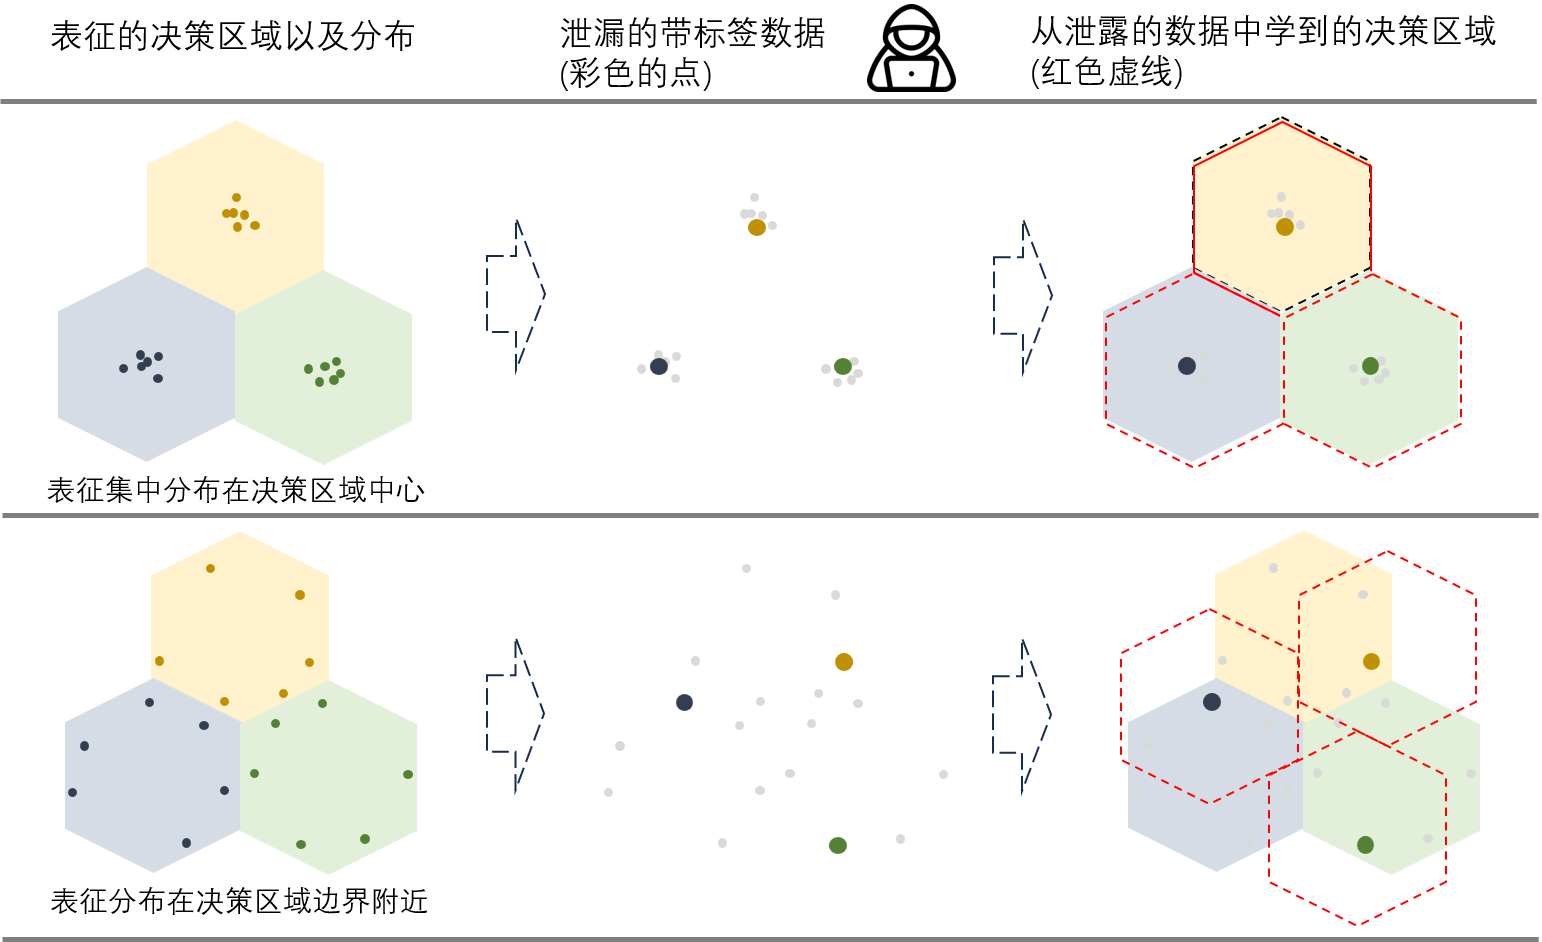
\includegraphics[width=1\linewidth]{Z_Resources/peloss_method.png}
    \caption{隐层表征分布导致的攻击者误差示意图}
    \label{fig:peloss:method}
\end{figure}


\subsection{势能损失函数定义}
物理学中的静电平衡(Electrostatic Equilibrium)现象告诉我们,当一个导体建立静电平衡时,其所有净电荷(Net Charge)将会分布在导体表面~\cite{griffiths2005introduction}。
%
这个现象的一部分原因时库仑定律(Coulomb's Law),即:同性电荷之间相互排斥,而异性电荷之间相互吸引。
%
受到该物理现象的启发,我们可以把相同类别的表征看作同性电荷,使得它们之间存在互相排斥对方的斥力。
因此,这些同类别的表征就会相互远离直到决策区域的边界处。
%

库仑定律的公式为
\begin{equation}
\label{eq:peloss:columb}
    \bvec{F} =  k {q_1q_2(\bvec{r}_1 - \bvec{r}_2)}/{\Vert r_1 - r_2 \Vert_2^3},
\end{equation}
其中,$k$表示一个常数,$q_1, q_2$是带符号的电荷大小(正电荷为正号,负电荷为负号),$\bvec{r}_1, \bvec{r}_2$表示两个电荷的位置,$\Vert \cdot \Vert$表示欧几里得范数,$\bvec{F}$则表示第二个电荷对第一个电荷产生的力(库仑力)的大小。
%
我们忽略常数以及电荷的大小,只考虑同性电荷,则可以把\autoref{eq:peloss:columb}化为$\bvec{F} = (\bvec{r}_1 - \bvec{r}_2) / \Vert\bvec{r}_1 - \bvec{r}_2 \Vert_2^3$。
%
由于库仑力也可以表示为电势能的梯度,我们可以进一步将其表示为梯度的形式$F = \nabla_{\bvec{r}_1} 1/\Vert \bvec{r}_1 - \bvec{r}_2 \Vert_2$。
%
这种表示方法与深度学习中所使用的梯度下降方法不谋而合。
%
基于以上分析,我们定义势能损失函数为:
\begin{equation}
    L_\text{pe} = \sum\limits_{c\in\mathcal C}\sum\limits_{\bvec{h} \in H_c}\sum\limits_{\bvec{h}' \in H_c, \bvec{h}' \ne \bvec{h}} \dfrac{1}{\Vert \bvec{h} - \bvec{h'} \Vert_2},
\end{equation}
其中$\mathcal C$表示标签的集合,$H_c$表示类别为$c$的表征集合。


通过把$L_{pe}$加入损失函数中,在拆分模型的训练过程中,同类别的表征互相之间会排斥并且逐渐移动到该类别的决策区域边界处。
%
在三维的情况下,汤姆森定理(Thomson's Theorem)证明电势能最小的情况对应于电荷全部分布在导体的表面~\cite{thomson_1913_atom,bakhoum_2008_thomson_proof},也就是此时表征的概率质量全部在决策边界。
%
但是考虑到拆分层的表征空间的维度一般远大于3维,因此其概率质量并不能完全集中在决策边界。
但是我们依然能证明,在势能损失函数最小的情况下,决策边界处必然有概率质量分布。

\begin{theorem}[决策边界的表征分布非零]
\label{thm:peloss:border-distribution}
    考虑一个$d$维有界区域$\Omega \subset \mathbb R^d$以及定义在$\Omega$内部的概率密度泛函$f^*$为最小化势能损失的概率密度:
    \begin{equation}
        \label{eq:peloss:potential-min}
        f^* = \mathop\textnormal{argmin}_f \textnormal{PE}(f) = \mathop\textnormal{argmin}_{f} \int_{\bvec{x} \in \Omega} \int_{y \in \Omega} \dfrac{f(\bvec{x})f(\bvec{y})}{\Vert \bvec{x} - \bvec{y} \Vert_2} dUdV,
    \end{equation}
    其中,$f$表示概率密度函数且满足$f \ge 0$(非负性) 以及 $\int_{\Omega} f(\bvec{x})dV = 1$(归一性)。
    令$\Delta_\epsilon \Omega = \{\bvec{x}: \bvec{x} + \epsilon \bvec{r} \not\in \Omega, \bvec{x} \in \Omega, \Vert \bvec{r} \Vert_2 = 1 \}$ 表示距离$\Omega$边界距离小于$\epsilon$的区域,那么$f^*$满足对于任意$\epsilon > 0$,有$\int_{\bvec{x}\in\Delta_\epsilon \Omega} f^*(\bvec{x})dV > 0$。
\end{theorem}
\begin{proof}
    为了让证明过程更加清晰,此处我们用$|\cdot |$来表示欧几里得范数。
    %
    首先考虑中心在$\bvec{x}_0$,半径为$r$的球$B_r(\bvec{x}_0)$。
    令
    \begin{equation}
        r_0 = \inf_r \left\{ \int_{\bvec{y}\in \Omega - B_{r}(\bvec{x}_0)} f(\bvec{y}) dV = 0 \right\},
    \end{equation}
    即:$f(x)$ 在$B_{r_0}(x_0)$ 之外几乎处处为0,也就是说$B_0 = B_{r_0}(x_0)$是以$x_0$为中心且包含了几乎所有概率质量的最小半径球。
    %
    因此我们可以找到一个靠近$B_0$边界的小球$B_1 = B_{\epsilon/4}(\bvec x_0 + \bvec{r}')$使得
    $\int_{\bvec{y}\in B_1} f(\bvec{y})dV = \delta$,其中$\delta > 0$,$|\bvec{r}'| = r_0 - \epsilon / 4$。
    也就是说,$B_1$内部的概率质量非零。
    %

    现在我们考虑将$f$在$B_1$里面的概率质量移动到$B_2 = B_{\epsilon/4}(\bvec x_0 + \bvec{r}'(1 + \dfrac{3\epsilon}{4|r'|})) = B_{\epsilon/4}(\bvec x_0 + \bvec{r}'')$中。
    %
    由于$B_2 \subset \Delta_\epsilon \Omega$且$B_1 \subset \Omega - \Delta_\epsilon \Omega$,所以上述的移动是可行的。
    %
    我们把概率质量移动后的概率密度函数记作
    \begin{equation}
        f'(\bvec{t}) = \begin{cases}
            f(\bvec{t} - \bvec{r}'' + \bvec{r}') & \quad \text{当 $\bvec{t} \in B_2$},\\
            0               & \quad \text{当 $\bvec{t} \in B_1$},\\
            f(t)            & \quad \text{其他}.
        \end{cases}
    \end{equation}
    此时我们计算$f'$和$f$的势能差异(把$\Omega - B_1 - B_2$记作$\Omega'$,并注意到$f'$和$f$在$\Omega'$内部的概率质量产生的势能差异为零):
    \begin{equation}
    \label{eq:peloss:diff0}
    \small
    \begin{split}
        & \text{PE}(f) - \text{PE}(f') 
        = \int_{\bvec{x} \in \Omega} \int_{\bvec{y} \in \Omega} \dfrac{f(\bvec{x})f(\bvec{y}) - f'(\bvec{x})f'(\bvec{y})}{|\bvec{x}-\bvec{y}|}dUdV 
        \\
        & = 
        \left( 
            \int_{\bvec{x} \in B_1 \cup B_2} \int_{\bvec{y} \in \Omega'} + 
            \int_{\bvec{x} \in \Omega'} \int_{\bvec{y} \in B_1 \cup B_2} +
            \int_{\bvec{x} \in B_1 \cup B_2} \int_{\bvec{y} \in B_1 \cup B_2}
        \right) 
        \dfrac{f(\bvec x)f(\bvec y) - f'(\bvec x)f'(\bvec y)}{|\bvec x - \bvec y|}dUdV
        \\
         & = 2 \int_{\bvec x \in B_1} \int_{\bvec y \in \Omega'} \dfrac{f(\bvec x)f(\bvec y)}{|\bvec x-\bvec y|}dUd -
             2 \int_{\bvec x \in B_2} \int_{\bvec y \in \Omega'} \dfrac{f'(\bvec x)f(\bvec y)}{|\bvec x-\bvec y|}dUdV + \\
            &\quad 
            \int_{\bvec x \in B_1} \int_{\bvec y \in B_1} \dfrac{f(\bvec x)f(\bvec y)}{|\bvec x-\bvec y|}dUdV -
            \int_{\bvec x \in B_2} \int_{\bvec y \in B_2} \dfrac{f'(\bvec x)f'(\bvec y)}{|\bvec x-\bvec y|}dUdV.
    \end{split}
    \end{equation}
注意到$f'$是把$f$在$B_1$处的值直接移动到了$B_2$,因此上式最后两项可以相消。
此时可以把\autoref{eq:peloss:diff0}写成:
\begin{equation}
\label{eq:peloss:diff1}
        \dfrac{1}{2}[\text{PE}(f) - \text{PE}(f')] =
        \int_{\bvec x \in B_1} \int_{\bvec y \in \Omega'} \dfrac{f(\bvec x)f(\bvec y)}{|\bvec x- \bvec y|}dUdV
        -
        \int_{\bvec x \in B_2} \int_{\bvec y \in \Omega'} \dfrac{f'(\bvec x)f(\bvec y)}{|\bvec x- \bvec y|}dUdV.
\end{equation}
令$g(\bvec{s}) = f(\bvec{x} - \bvec{r}') = f'(\bvec{x} - \bvec{r}''), \bvec s \in B_{\epsilon/4}(0)$,则可以讲上式进一步简化为
\begin{equation}
\label{eq:peloss:diff2}
    \int_{\bvec x \in B_{\epsilon/4}(0)}\int_{\bvec y \in \Omega'} g(\bvec x)f(\bvec y) \left[ \dfrac{1}{|\bvec x + \bvec r' - \bvec y|} - \dfrac{1}{|\bvec x + \bvec r'' - \bvec y|} \right]dUdV.
\end{equation}
由于$\bvec r'$ 和 $\bvec r''$ 方向一致(我们将其对应的单位向量记作$\bvec e_r$),因此我们可以将$\bvec x$和$\bvec y$分解为与$\bvec e_r$相同的方向和与其正交的方向:
\begin{equation}
    \begin{cases}
        \bvec x_r = (\bvec x \cdot \bvec e_r) \bvec e_r \\
        \bvec x_v = \bvec x - \bvec x_v
    \end{cases} 
    \quad \text{以及} \quad
    \begin{cases}
        \bvec y_r = (\bvec y \cdot \bvec e_r)\bvec e_r \\
        \bvec y_v = \bvec y - \bvec y_v
    \end{cases}
\end{equation}
于是我们有:
\begin{equation}
\begin{cases}
    |\bvec x + \bvec r' - \bvec y|^2 & = |\bvec x_r + \bvec y_r|^2 + |\bvec x_r + \bvec r' - \bvec y_r|^2 
     = |\bvec x_v + \bvec y_v|^2 + |\bvec x_r + \bvec r' - \bvec y_r|^2, \\
    |\bvec x + \bvec r'' - \bvec y|^2 & = |\bvec x_v + \bvec y_v|^2 + |\bvec x_r + \bvec r'' - \bvec y_r|^2
    = |\bvec x_r + \bvec y_r|^2 + |\bvec x_r + \bvec r'' - \bvec y_r|^2,
\end{cases}
\end{equation}
上式最后一项的左侧是相等的,因此只需考虑右侧。
我们只需考虑考虑如下两种情况:
\begin{itemize}
    \item $|\bvec x_r + \bvec r'| \ge |\bvec y_r|$: 
    同时注意到 $|\bvec r''| > |\bvec r'|$,因此$|\bvec x + \bvec r'' - \bvec y| < |\bvec x + \bvec r' - \bvec y|$。
    \item $|\bvec x_r + \bvec r'| < |\bvec y_r|$:
    因为$|\bvec y_r| < r_0$,$|\bvec x_r + \bvec r'| \ge r_0 - \epsilon / 2$,以及$|\bvec x_r + \bvec r''| > r_0 + \epsilon / 2$,因此有
    \begin{equation}
        |\bvec x_r + \bvec r'' - \bvec y_r| > \epsilon / 2 > |\bvec y_r - (\bvec x_r + \bvec r')|.
    \end{equation}
\end{itemize}
综上,当$x \in B_{\epsilon/4}(0), y \in \Omega'$时,就有
\begin{equation}
    |\bvec x + \bvec r' - \bvec y| < |\bvec x + \bvec r'' - \bvec y|,
\end{equation}
因此,
\begin{equation}
    1 / |\bvec x + \bvec r' - \bvec y| - 1 / |\bvec x + \bvec r'' - \bvec y| > 0.
\end{equation}
带入\autoref{eq:peloss:diff2},可以得到$\text{PE}(f') < \text{PE}(f)$。
至此\autoref{thm:peloss:border-distribution}得到证明。
\end{proof}

\autoref{thm:peloss:border-distribution}表明,当势能损失最小时,表征在决策边界上的分布必然不为0,否则我们便可以通过移动一小部分的概率质量到边界处使得势能损失更小,与势能损失最小的前提相矛盾。

\textbf{加入层归一化}:
势能损失方法有一个隐含条件:某一类别的表征的决策区域需要是有界的,并且要与其他类别的表征决策区域相邻。
否则,势能损失可以把同类表征推向无穷远处或是与其他类别决策区域不相邻的“边界”,使得其保护能力降低。
%
这要求表征空间是一个有界(Bounded)并且无边界(Borderless)的流形。
%
我们简单地通过层归一化(Layer Normalization)~\cite{hinton_2016_layernorm}来实现该要求。
%
经过层归一化后,拆分层的表征被投影到$d$维超球体上。
%
为了保持一致性,我们也需要改变其距离的计算方式,将欧氏距离(Euclidean Distance)转化为超球面上的测地距离(Geodesic Distance),此时势能损失函数被修改为:
\begin{equation}
    L_\text{pe} = \sum\limits_{c\in\mathcal C}\sum\limits_{\bvec{h} \in H_c}\sum\limits_{\bvec{h}' \in H_c, \bvec{h}' \ne \bvec{h}} {1}/{\arccos \left({\bvec h \cdot \bvec h'} \over {\Vert \bvec h \Vert_2 \cdot \Vert \bvec h' \Vert_2}\right)}.
\end{equation}
%

最终,在模型的训练过程中,我们把势能损失加入到原有的损失函数(如交叉熵分类损失)中,并设置权重为$\alpha$。
总的损失函数为$L' = L + \alpha L_{pe}$。

\subsection{与距离相关性的关系}
已有研究采用了距离相关性将拆分层表征对输入特征~\cite{vepakomma2020nopeek}或预测标签~\cite{sunjiankai2022forward_embedding_protect}进行解耦,从而保护输入特征或标签。
%
我们在这里讨论对标签进行保护的情况,此时距离相关性损失可以表示为
\begin{equation}
\label{eq:peloss:dcorloss}
    L_\text{dcor} = \sum_{i=1}^n d_{i,j} d'_{i, j} \Big/ \sqrt{\sum_{i,j=1}^n d_{i, j}^2 \sum_{i,j=1}^n {d'}_{i, j}^2},
\end{equation}
%
其中,$d_{i,j}$表示样本$i$和样本$j$的表征之间的双中心(Doubly-Centered)距离,即:
\begin{equation}
    d_{i, j} = \Vert \bvec h_i - \bvec h_j \Vert_2 - \mathop{\mathbb E}_{\bvec h'\in H}\Vert \bvec h_i - \bvec h' \Vert_2 - \mathop{\mathbb E}_{\bvec h'\in H}\Vert \bvec h' - \bvec h_j \Vert_2 + \mathop{\mathbb E}_{\bvec h', \bvec h'' \in H}\Vert \bvec h' - \bvec h'' \Vert_2.
\end{equation}
%
类似地,$d'_{i,j}$则是样本$i$和样本$j$的标签的双中心距离,以独热(One-Hot)标签为例,当$i,j$标签不同时$d_{i,j} = \sqrt 2$。
将其带入\autoref{eq:peloss:dcorloss},提取出其分母,得到
\begin{equation}
    \sum_{\substack{c,c'\in \mathcal C \\ c\ne c'}} \sum_{\substack{\bvec h\in H_c \\ \bvec h' \in H_c'}} \sqrt2 
    \left( 
        \Vert \bvec h - \bvec h'\Vert_2 - \overline{\Vert \bvec h - \cdot \Vert_2} - \overline{\Vert \bvec \cdot - \bvec h' \Vert_2} + \overline{\Vert \cdot - \cdot\Vert_2}, 
    \right)
\end{equation}
其中,我们用 $\overline{\Vert \bvec h - \cdot \Vert_2}$ 表示 $\mathbb E_{\bvec h'\in H} \Vert \bvec h - \bvec h'\Vert_2$,$\overline{\Vert \cdot - \cdot \Vert_2}$ 表示 $\mathbb E_{\bvec h, \bvec h'\in H} \Vert \bvec h - \bvec h'\Vert_2$,$H$表示当前批样本表征集合,$H_c$表示当前批样本中类别为$c$的表征集合。
%
可以看出最小化距离相关性损失类似于最小化表征的类间距离,而本文提出的势能损失则旨在最大化类内距离,两者之间有一定的相似性。
%
然而直观地来讲,不同类别的决策边界分布在不同的方向上,导致距离相关性的计算有更高的误差且难以优化。
%
后续的实验结果也表明势能损失相比于距离相关性更加优越。


\subsection{输入特征的隐私保护}
势能损失虽然没有直接保护输入特征的隐私,但是间接地对其进行了保护。
%
这是因为在拆分学习中,可以通过拆分层位置的选择来调节输入特征和标签的隐私泄露程度。
具体而言,拆分层靠近模型输入,则输入特征隐私泄露加大;而拆分层靠近模型输出,则输出特征隐私泄露加大~\cite{abuadbba2020can_split}。
%
而通过势能损失函数,我们可以将拆分层设置到更靠近输出的位置,此时输入特征的隐私泄露自然也就减少了。
%
尤其是对于基于卷积神经网络或Transformer的模型,在无保护的情况下,其中间层会保留大量的输入数据的信息。
通过势能损失,可以把拆分层设置为最后一层,极大提高对于输入特征的保护,同时也保护标签的隐私。
%
\section{实验分析}
为了验证本文所提出的势能损失函数对于模型补全攻击的有效性,本文在多个数据集上进行了实验,并且与距离相关性损失~\cite{vepakomma2020nopeek,sunjiankai2022forward_embedding_protect}以及标签差分隐私(Label Differential Privacy)~\cite{wuruihan_2023_label_dp}的方法进行对比。
%
各个数据集和对应的模型介绍如下:
\begin{itemize}
    \item MNIST~\cite{mnist}:一个常用的手写数字数据集,是一个10分类的手写数字分类数据集,包含了60000个训练样本和10000个验证样本,每个样本为$28\times 28$的灰度图片。
    对应的模型是一个隐层大小为[128, 32]的全连接神经网络,激活函数采用LeakyReLU。
    
    \item Fashion-MNIST~\cite{fashion}:一个包含了10个类别的图片数据集,包含了7万张服饰相关的$28\times 28$大小的黑白图片。
    对应的模型是一个双层卷积加上双层全连接的模型,卷积层的通道数分别为[32, 64],卷积核大小分别为$[5, 3]$,每一个卷积层后面跟随LeakyReLU激活函数和大小为2的最大池化层。
    全连接层的维度为2304(卷积层提供的输入)-128-10(输出)。
    
    \item CIFAR-10~\cite{krizhevsky_2009_cifar}:一个包含了10个类别的6万张图片的彩色图片数据集,图片大小为$3\times 32\times 32$。
    对应的模型是ResNet-20模型~\cite{hekaiming2016resnet}。

    \item DBPedia~\cite{2007dbpedia}:一个文本分类数据集,在第\ref{chap:randomized_topk}章已经进行了介绍。
    我们采用TextCNN模型~\cite{kimyoon2014textcnn}进行分类,卷积核的大小为 $(3,4,5)$,并且使用Glove预训练词向量~\cite{pennington2014glove}。
    拆分层设置为最后的隐层,大小为300。
\end{itemize}
%

攻击者采用微调攻击和聚类攻击两种方法对训练完成的拆分学习模型进行攻击。
对于微调攻击,当拆分层为最后一层的时候,攻击者使用同类样本表征均值来初始化最后一层的权重。
对于聚类攻击,我们采用经典的$k$-平均($k$-Means)聚类算法~\cite{macqueen1967kmeans},并且给定类别个数。

所有实验都在装配有NVIDIA RTX 3090 GPU的服务器上进行,并使用不同的随机种子重复5次以上。
%
对于所有的任务,我们最多训练100轮模型,并在90-100轮中采用“早停(Early Stopping)”策略获取验证集最佳的模型,以保证原始损失函数和额外损失函数均被充分优化。
%
对于聚类攻击,我们采用Scikit-Learn库~\cite{pedregosa_2011_scikit}中的$k$-平均聚类算法,并采用默认参数。
%
我们将势能损失的权重从0.25变化到32,每次翻倍;
类似地,对于距离相关性损失,我们也把权重从1变化到32,每次翻倍;
对于标签差分隐私方法,我们将翻转的标签比例从0.01提高到0.16,每次翻倍。
%
我们默认将拆分层选为模型的最后一层,因为其最贴近模型的输出,但我们也汇报了拆分层选为其他层的实验结果。
%



\subsection{微调攻击}

我们测量了模型在测试集上的准确率,以及攻击者在泄漏的带标签数据上进行微调攻击得到的模型的准确率。
我们将拆分层为最后一层的结果和拆分层为中间其他层的结果分别汇报在\autoref{fig:peloss:fine-tuning}和\autoref{fig:peloss:fine-tuning-middle}中。
%
在拆分中间其他层的实验中,我们将MNIST任务的全连接神经网络的拆分层设置在第一个隐层处,将CIFAR-10任务的拆分层设置在第二个残差块(Residual Block)之后。

图中的数据点的深浅对应实验中势能损失函数/距离相关性损失函数的系数或标签翻转概率,颜色越深代表超参数的设定越偏向于保护隐私,越浅则代表超参数的设定越偏向于保留原始任务的准确率。
%
落在灰色区域的数据表示训练好的拆分学习模型实现了完美保护,也就是底部模型或隐层表征对于攻击者没有任何额外作用,攻击者对其实行攻击的效果未达到在泄漏的数据集上直接训练的效果。
%
如果数据点落在图的左下角,说明该实验降低了攻击准确率的同时保持了原始任务的准确率。

实验结果表明,如果不对拆分学习加以防护,则攻击者可以获得很高的攻击效果。
%
标签差分隐私、距离相关性损失和势能损失都能一定程度上降低攻击准确率,且势能损失的数据点大多落在对比方法的右下方,表明势能损失取得了更好的保护效果的同时又有更高的原始任务准确率。
%
同时,势能损失数据点连成的曲线较为平滑,可以很清楚展现出通过改变损失系数来权衡原始任务准确率和攻击效果的过程。与此同时,距离相关性损失的数据点则难以连成曲线,表明其效果难以控制。
%
此外,势能损失有最多的数据点落在完美保护区域,而其他方法落在完美保护区域的数据点则很少。
%
综上,对于微调攻击,在同等的原始任务准确率下,势能损失的防御效果显著高于其他方法。

\begin{figure}[h!]
    \centering
    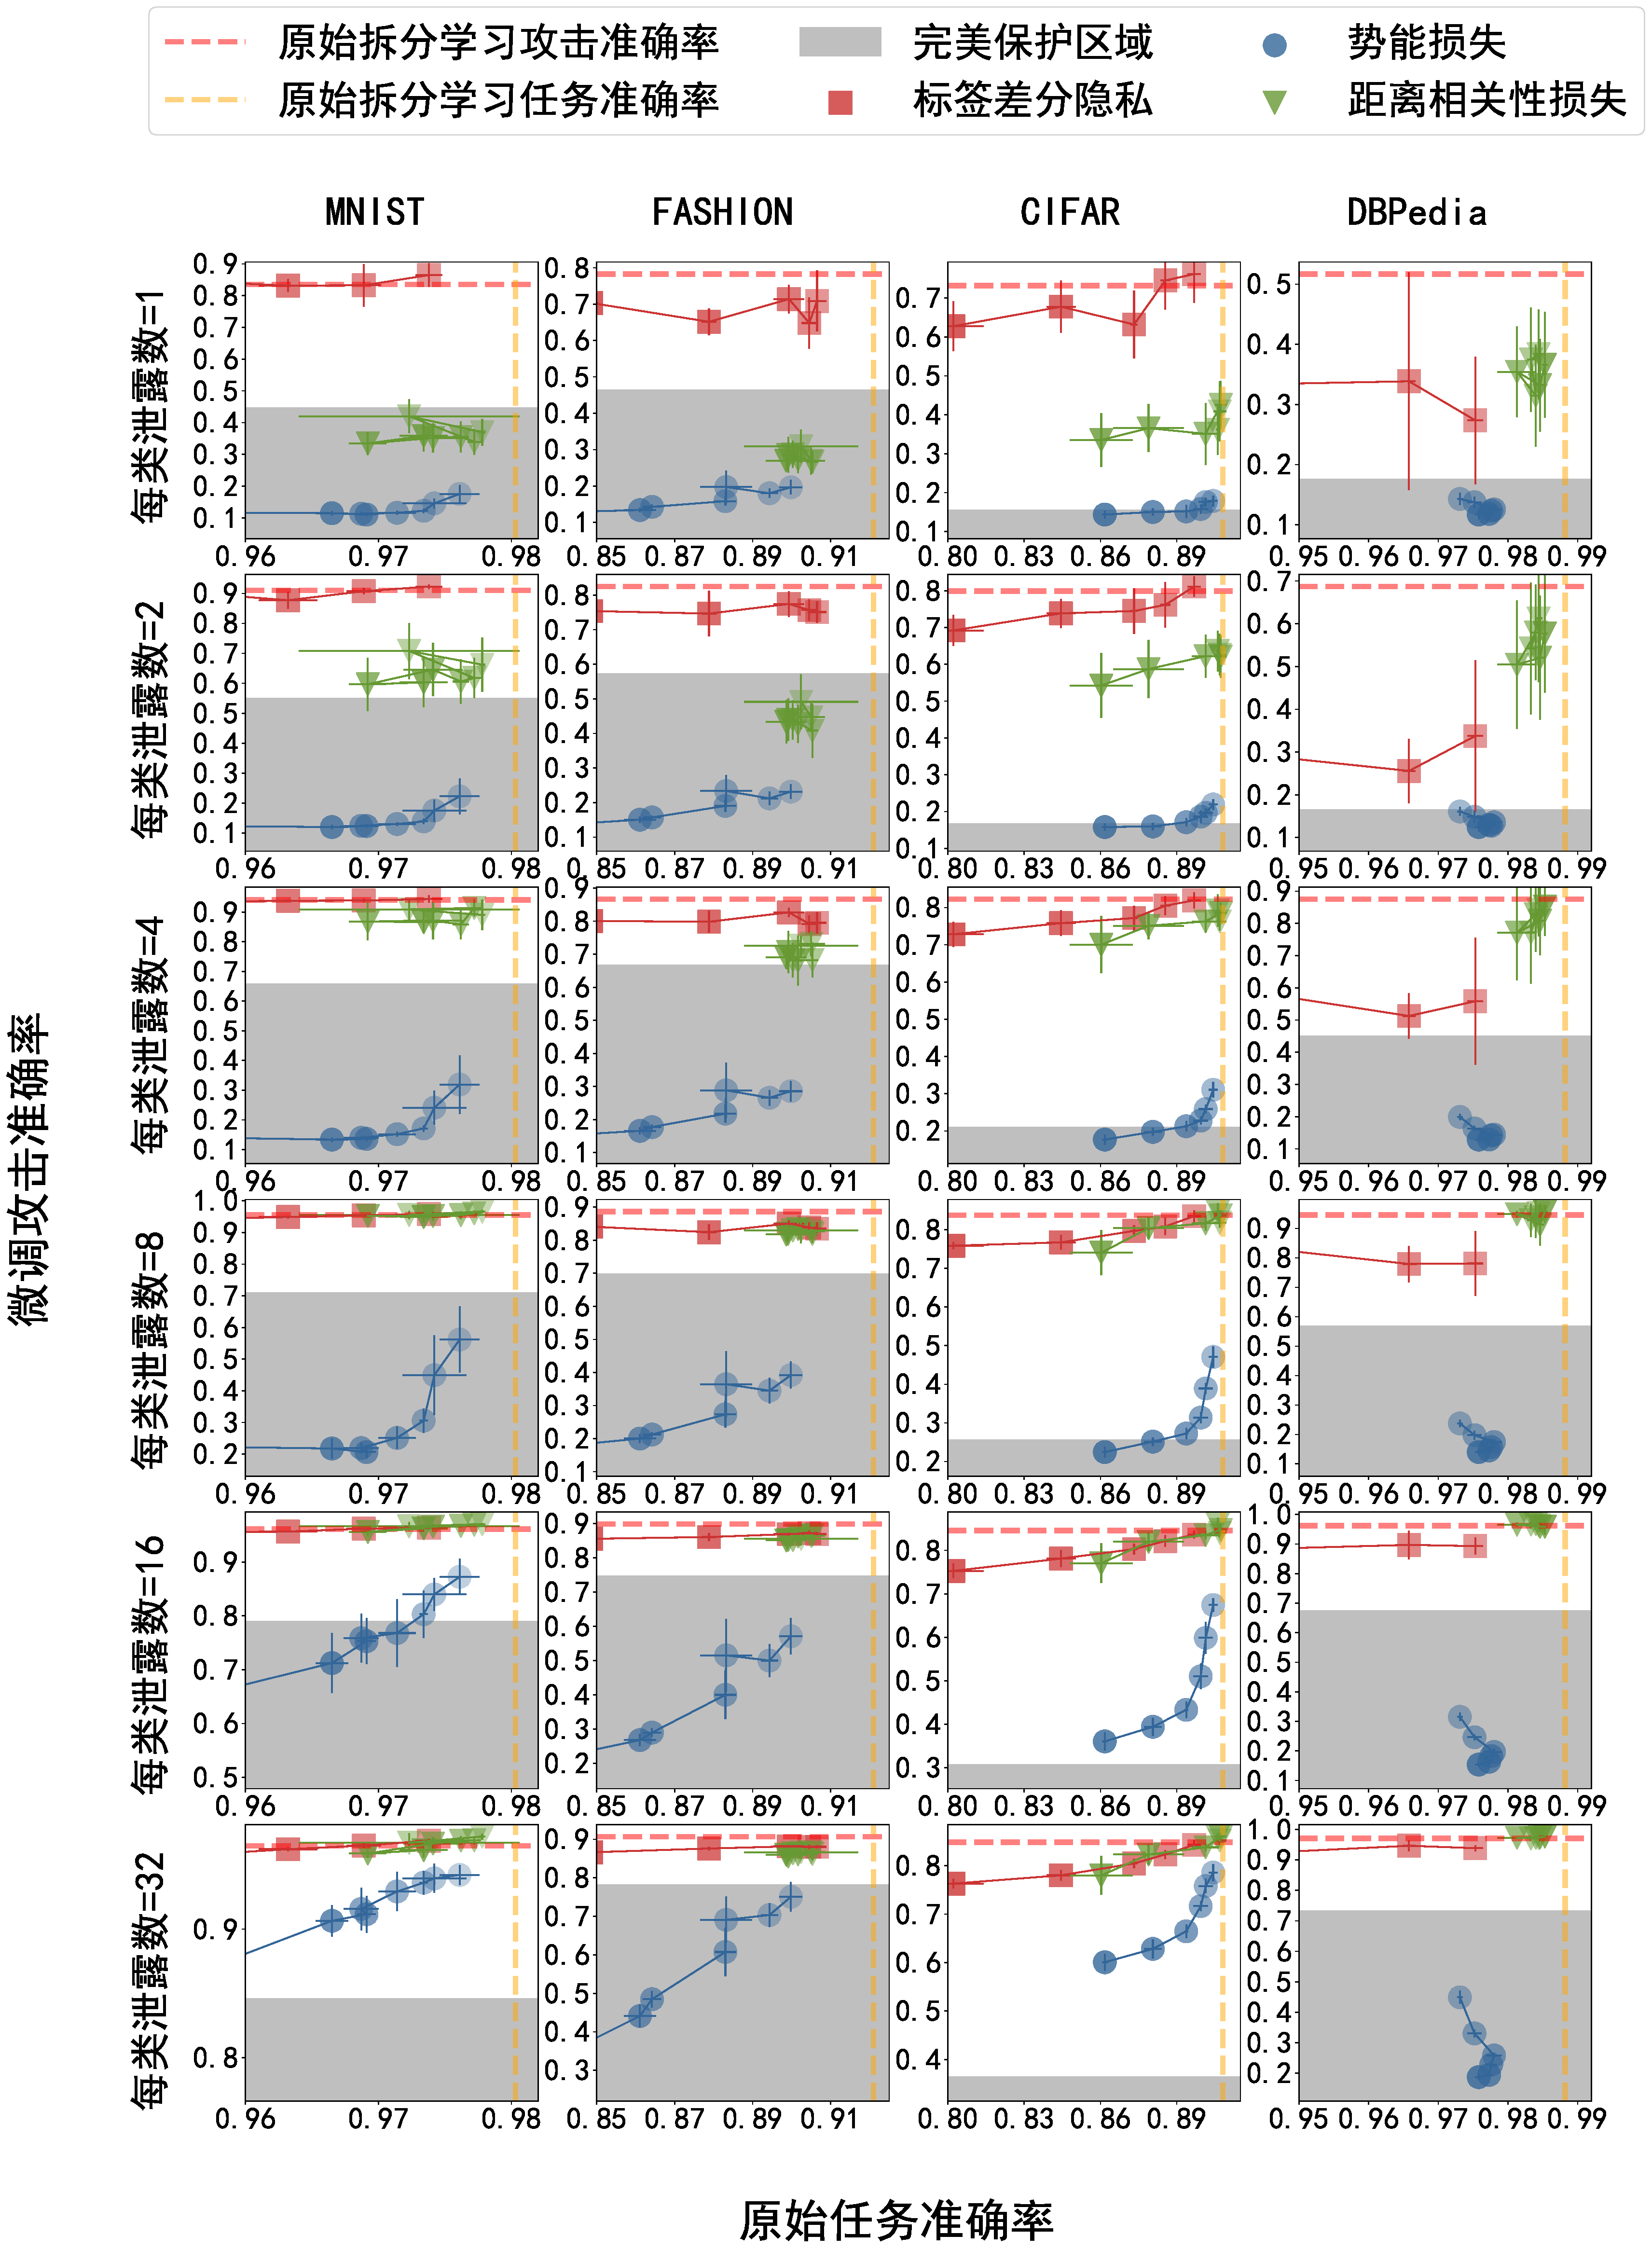
\includegraphics[width=1\linewidth]{Z_Resources/peloss_fine-tuning}
    \caption{拆分层为最后一层时原始任务准确率与微调攻击准确率对比图}
    \label{fig:peloss:fine-tuning}
\end{figure}


\begin{figure}[h!]
    \centering
    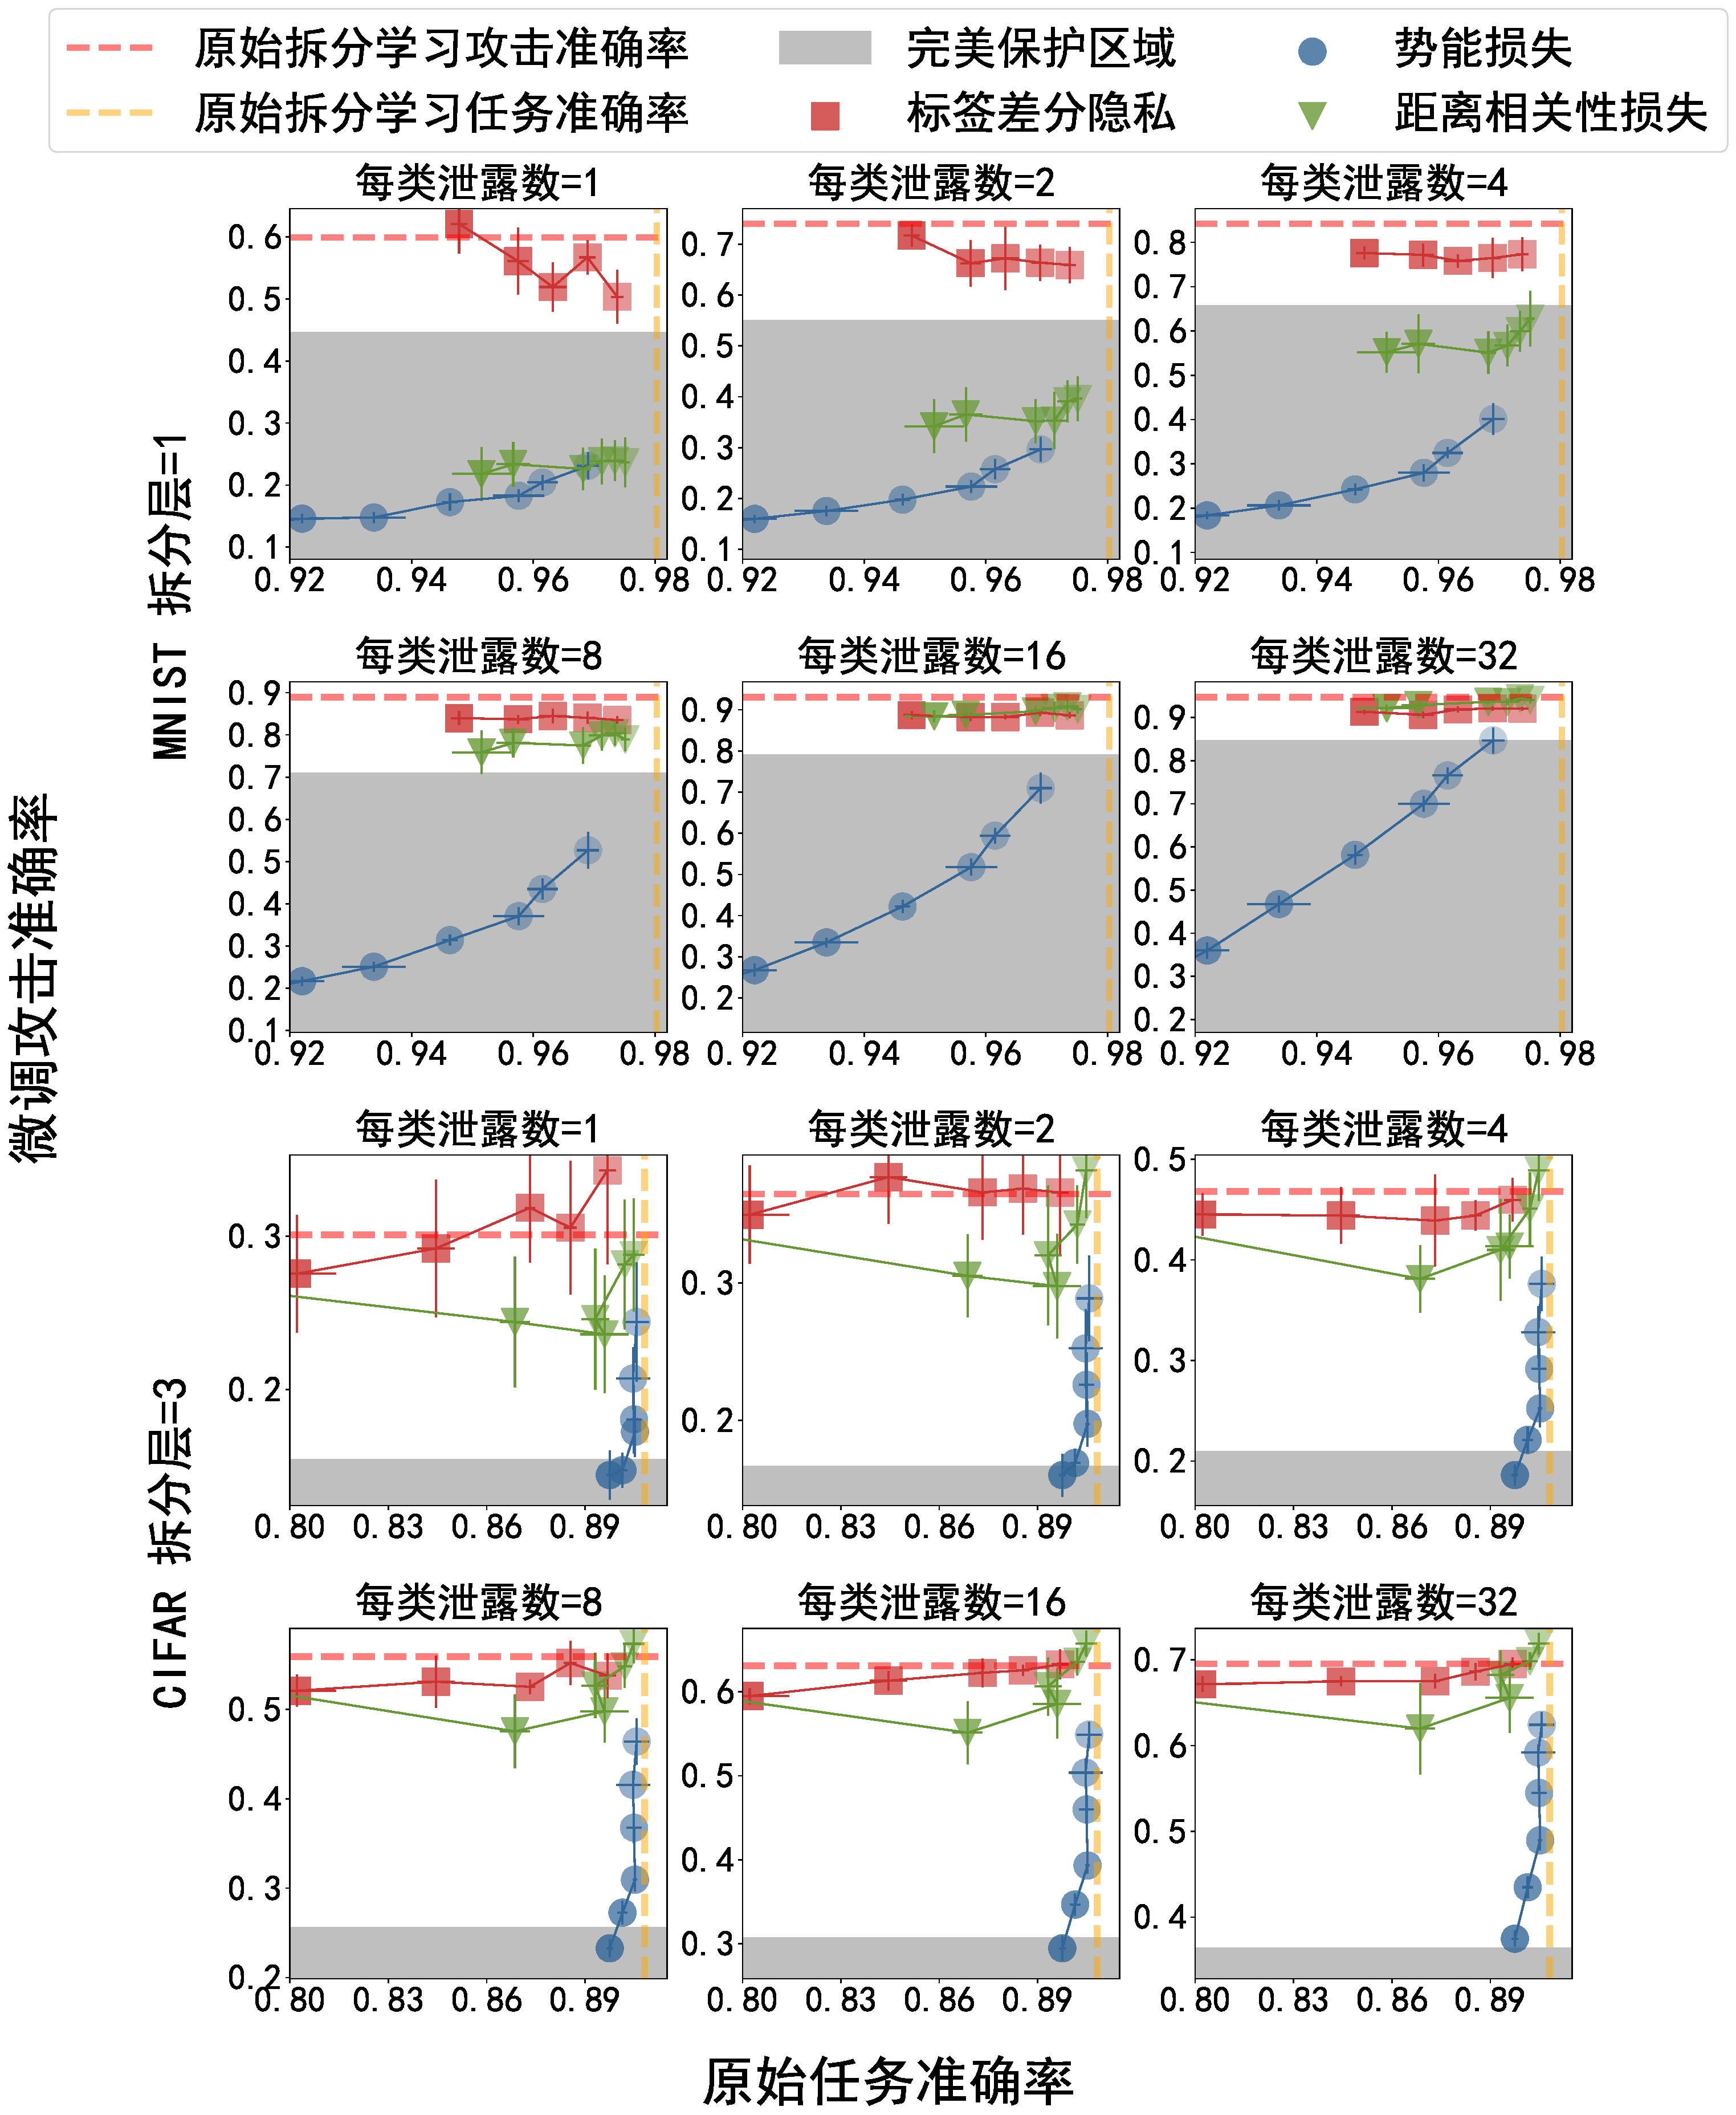
\includegraphics[width=0.85\linewidth]{Z_Resources/peloss_fine-tuning-middle}
    \caption{拆分层为中间层时原始任务准确率与微调攻击准确率对比图}
    \label{fig:peloss:fine-tuning-middle}
\end{figure}


\subsection{聚类攻击}
\begin{figure}[h!]
    \centering
    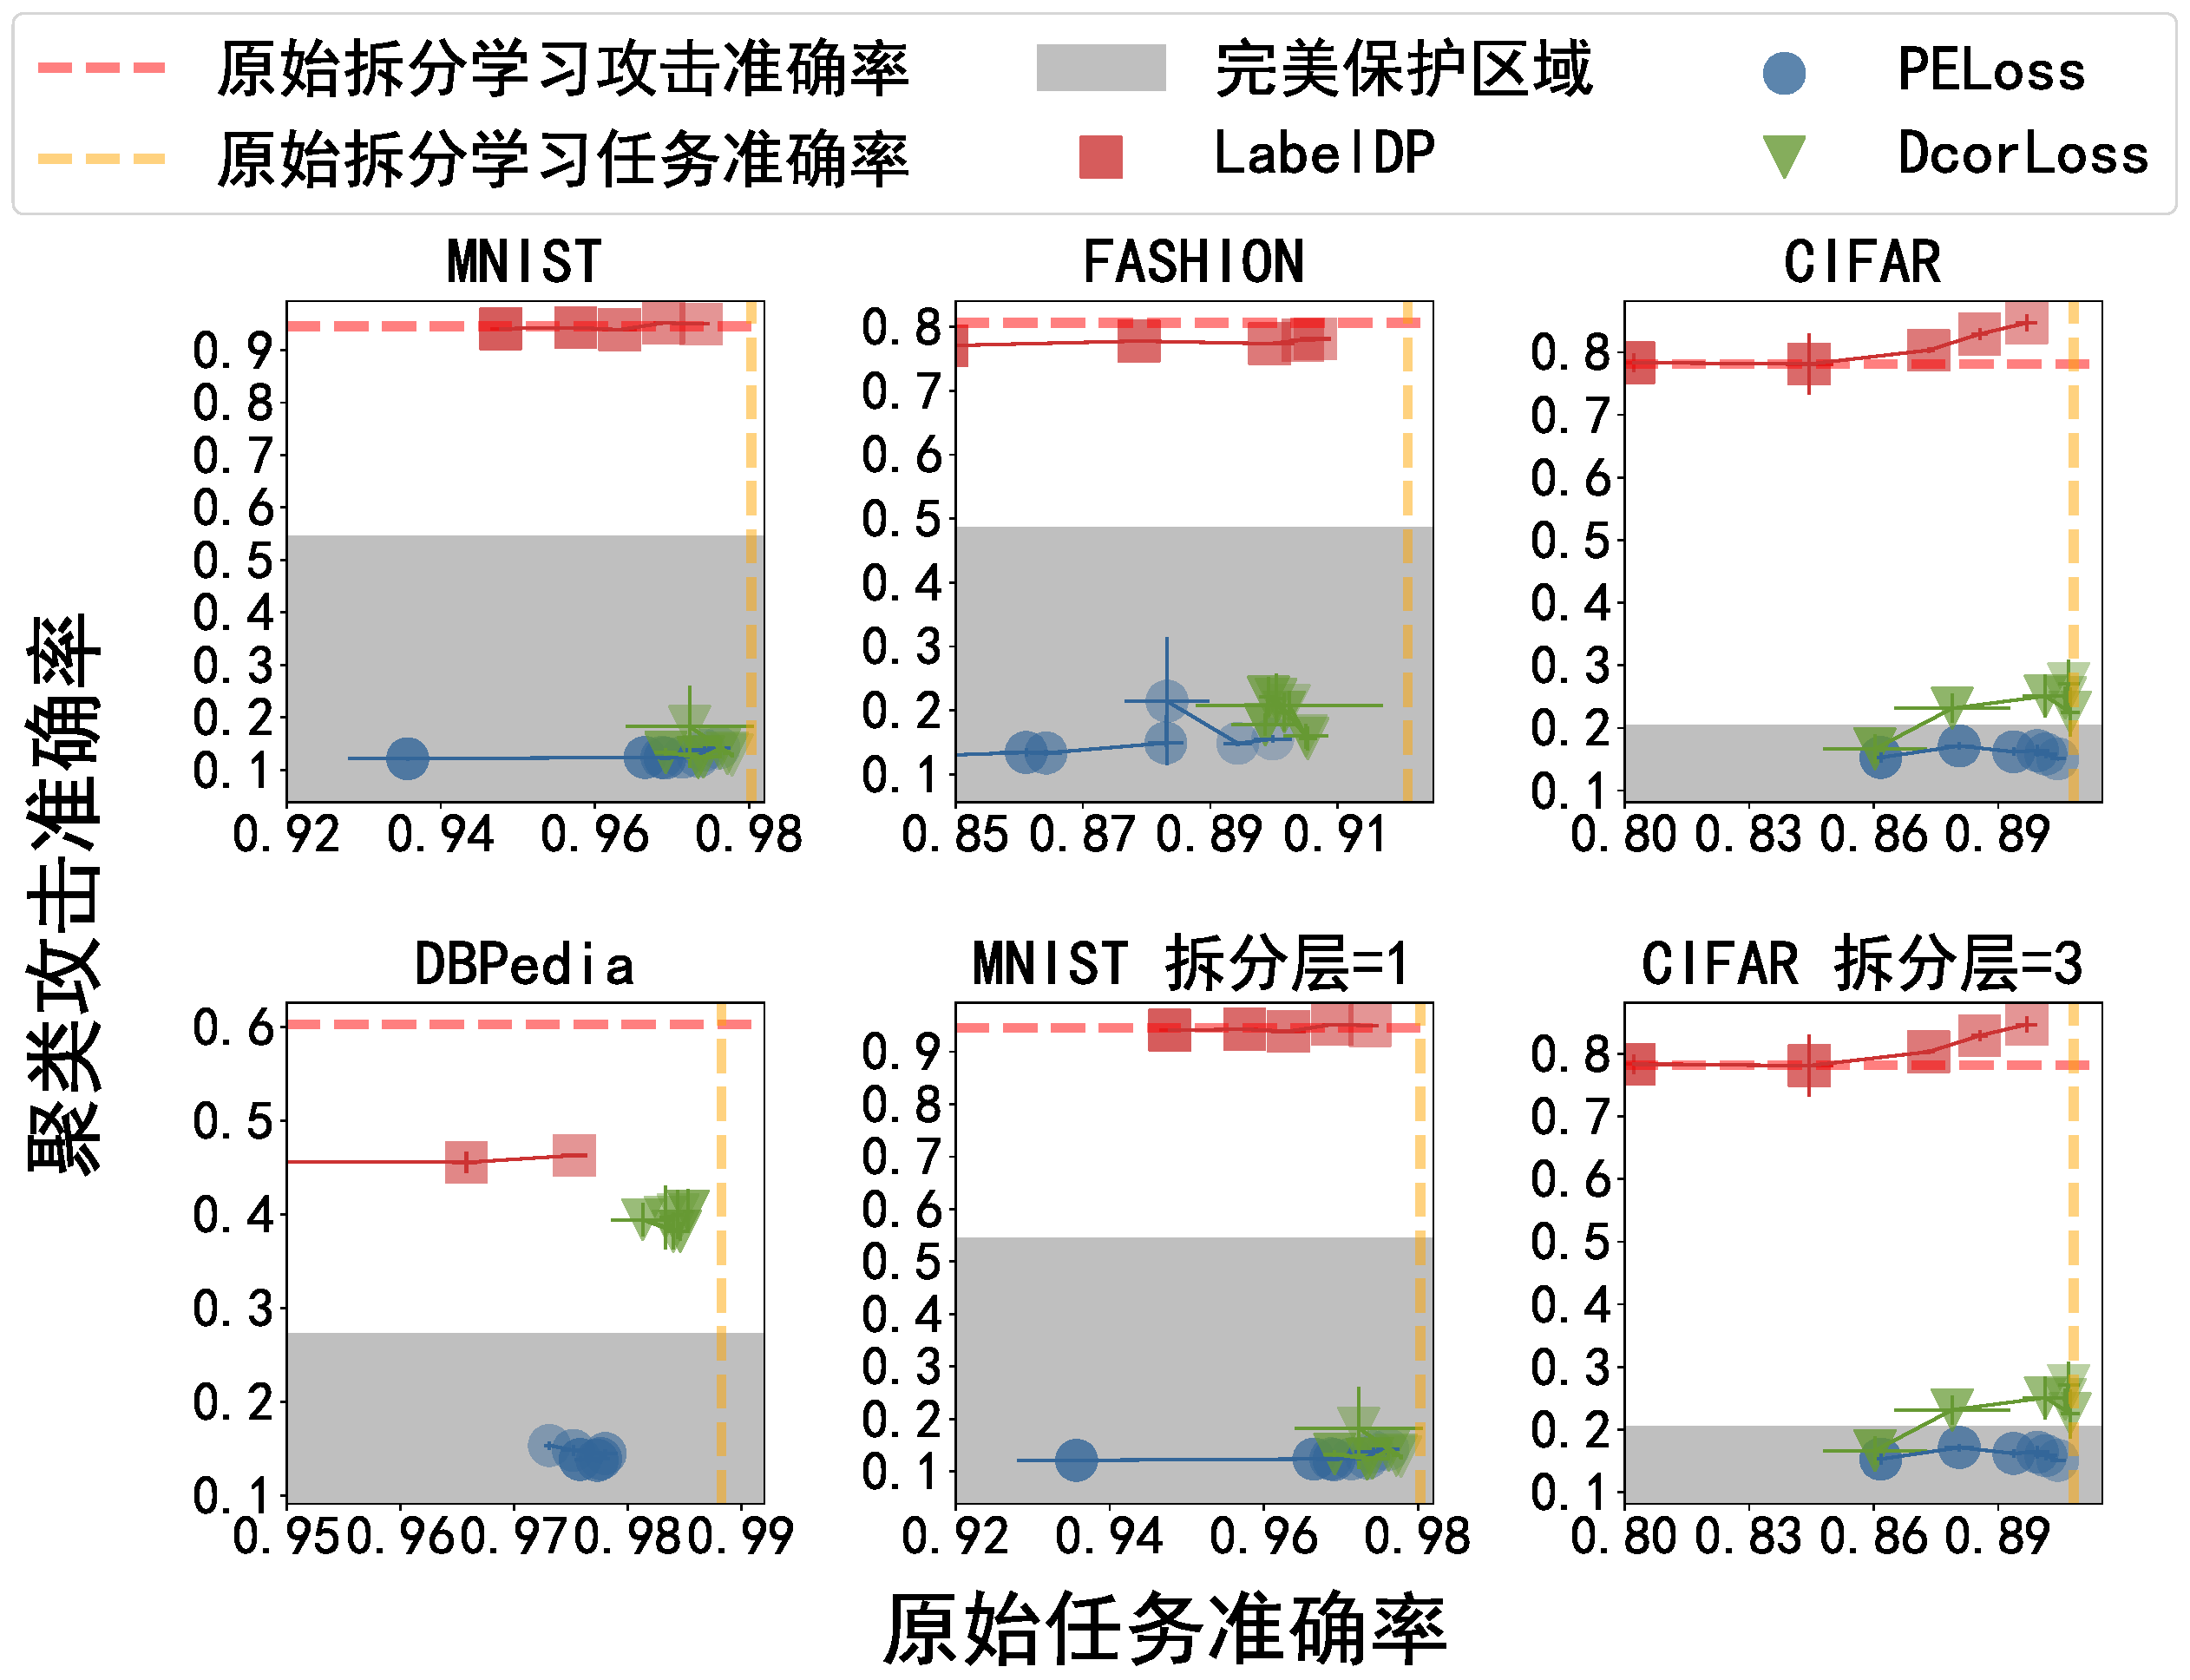
\includegraphics[width=0.8\linewidth]{Z_Resources/peloss_cluster-attack-both}
    \caption{原始任务准确率与聚类攻击准确率对比图}
    \label{fig:peloss:clustering}
\end{figure}

我们测量了模型在测试集上的准确率,以及攻击者无标签数据(整个测试集,均超过1万个样本)上进行聚类攻击得到的模型的准确率。
全部结果汇报在\autoref{fig:peloss:clustering}中。
%
由于聚类结果本身并不与实际的标签类别相对应,我们通过匈牙利匹配算法(Hungarian Matching Algorithm)~\cite{kuhn_1955_hungarian}找到准确率最高的类别映射关系并汇报该准确率。
该准确率计算公式可以表示为:
\begin{equation}
    \max\limits_{k_1,\cdots,k_C \in \text{Permutation}(1,\cdots,C)} \dfrac{\sum_{i=1}^C c_{i,k_i}}{\sum_{i,j=1}^C c_{i,j}},
\end{equation}
其中 $C$表示样本总数,$c_{i,j}$ 表示第 $i$ 个簇中实际标签是 $j$ 的样本数量, $1 < i, j \le C$。

%
实验结果表明,势能损失在所有的情况下均实现了完美保护,大幅领先于其他对比方法。
也就是说攻击者直接在泄漏的无标签数据上聚类得到的效果高于在拆分层表征上聚类得到的效果。
%
而标签差分隐私在对抗聚类攻击上效果不佳,相比于原始的拆分学习,未呈现出明显的保护作用。


\subsection{在拆分层之前攻击}
\begin{figure}[h!]
    \centering
    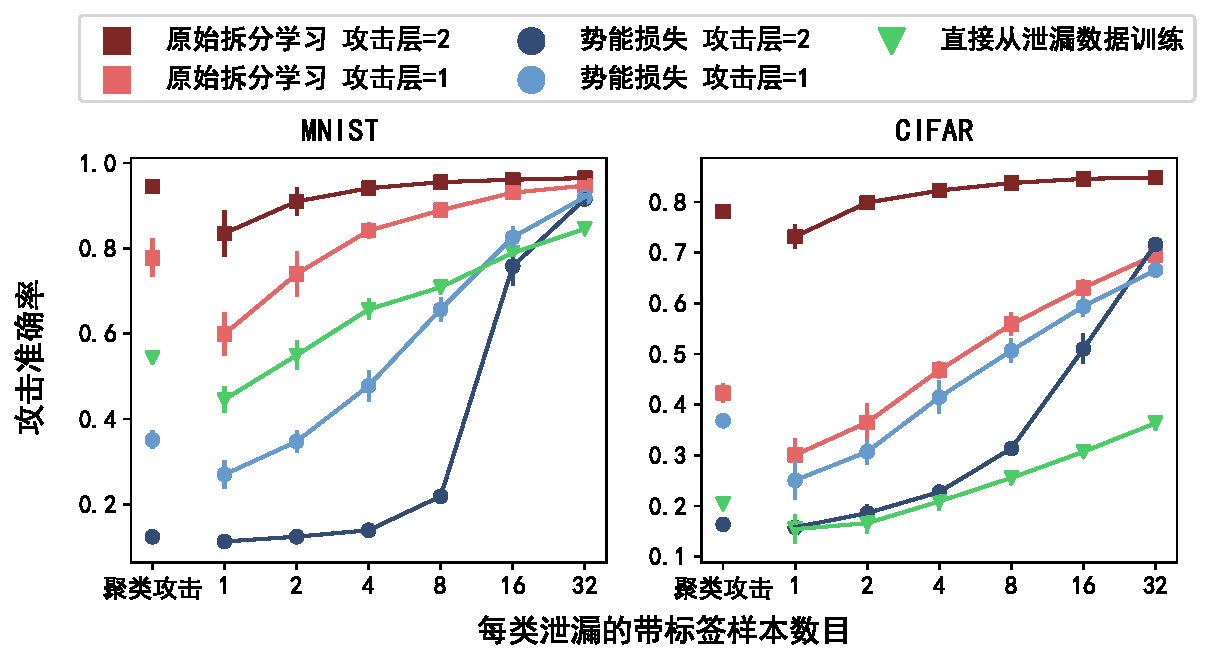
\includegraphics[width=0.85\linewidth]{Z_Resources/peloss_attack-layer}
    \caption{攻击层在拆分层之前时原始任务准确率与模型补全攻击准确率对比图}
    \label{fig:peloss:attack-layer}
\end{figure}

在之前的模型补全攻击实验中,我们假设攻击者使用了拆分层的表征进行攻击。
如果攻击者可以获取并操纵整个底部模型,则他也可以在拆分层之前的层进行攻击,也就是获取拆分层之前的隐层表征来微调模型或聚类。
%
因此,我们在MNIST和CIFAR任务中考察了攻击者在拆分层之前的层攻击的情况。
我们将拆分层设置为模型最后一个隐层,然后将MNIST任务的攻击层设置在第一个隐层处,将CIFAR-10任务的攻击层设置在第二个残差块(Residual Block)之后。
%
对于该实验,势能损失的系数被选取为$\alpha=4$。
%
我们在\autoref{fig:peloss:attack-layer}呈现在拆分层之前攻击的实验结果。

可以看到,在拆分层之前攻击可以让攻击效果有所提升,但是依然比无保护的拆分学习的攻击效果要低很多。
%
这是由于势能损失在训练过程中作用于拆分层的表征上而非之前的表征,因此拆分层之前的层的表征分布可能与标签关联性更大,使得攻击者更容易对其进行训练。

\subsection{拆分层维度的影响}
\begin{figure}[h!]
    \centering
    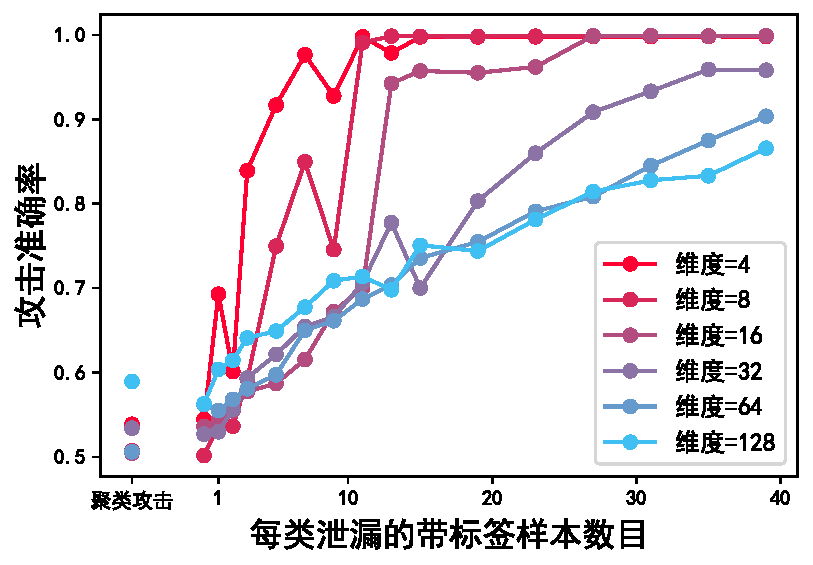
\includegraphics[width=0.7\linewidth]{Z_Resources/peloss_mnist-subclass2}
    \caption{拆分层维度对模型补全攻击准确率的影响}
    \label{fig:peloss:bottom_dim}
\end{figure}

为了研究拆分层的维度对于攻击效果的影响,我们对MNIST数据集的01子集上(只保留0和1类别的样本)进行了实验,其结果被汇报在\autoref{fig:peloss:bottom_dim}中。
此时我们设置势能损失的系数$\alpha=1$。

从图中可以看出,较高的拆分层维度大体上让微调攻击变得更难了,特别在每类样本泄露数较多的情况下。
%
例如,拆分层仅仅为4维的时候,只需要每个类别10个样本就可以让攻击准确率达到100;
而拆分层维度为128时,每类泄露40个样本后攻击准确率也不到90\%。
这是因为对更高维度的数据(也就是隐层表征)进行分类时,自然需要更多的样本。
%
作为对比,在聚类攻击时,更高的拆分层维度并未降低攻击的效果,甚至反倒有所提高。
这可能与聚类攻击时样本数量庞大有关。



\subsection{拆分层表征分布分析}
%
为了分析拆分层表征的分布,我们在MNIST数据集上计算了同类别表征之间和不同类别表征之间的角距离的分布,并且呈现在\autoref{fig:peloss:angular-distance} 中。
%
对于势能损失和距离相关性损失,我们分别把系数设置为$\alpha=1$和$\alpha=0.5$,这两者的原始任务效果基本相同。
%
图中可以看出,无论是否是同类别,抑或是属于训练集或者测试集,势能损失方法的样本表征间的角距离都接近$\pi/2$。
也就是说,无论两个表征是异类的或是同类的表征,它们都几乎相互正交。
%
对于距离相关性损失, 角距离则呈现出一个双峰分布,峰值靠近$0$和$\pi$。
并且同类别的样本表征对的角距离在靠近0的分布明显增加,导致保护效果变差。
%
而原始拆分学习中,同类别的表征之间的角距离则明显小于不同类别的表征之间的角距离,因此攻击准确率较高。


\begin{figure}[h!]
    \centering
    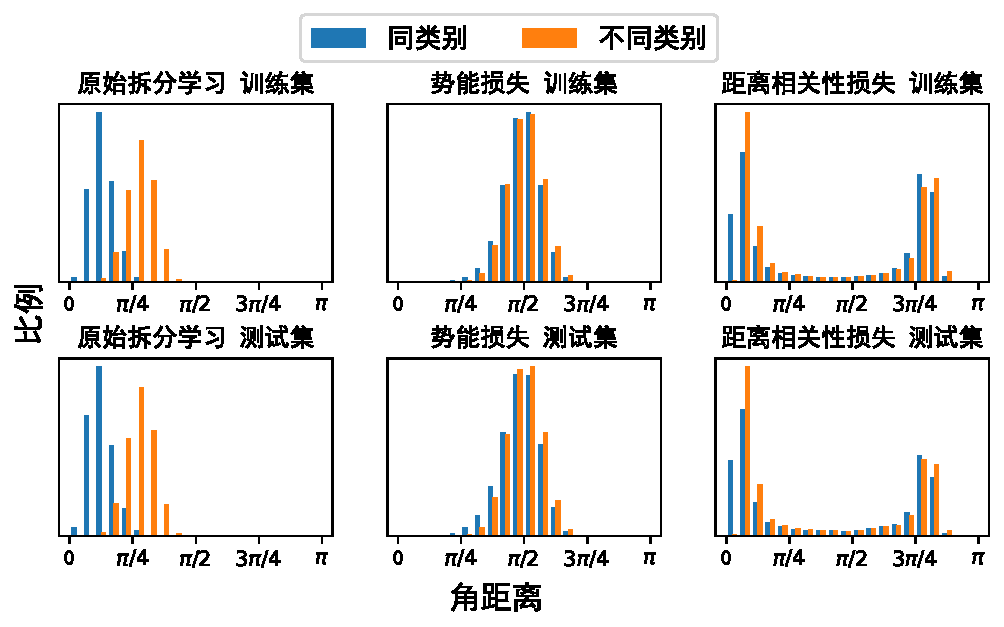
\includegraphics[width=0.8\linewidth]{Z_Resources/peloss_angular-distance}
    \caption{同类别和不同类别的隐层表征之间的角距离分布}
    \label{fig:peloss:angular-distance}
\end{figure}

为了更直观地呈现拆分层表征的分布,我们使用了t-SNE降维~\cite{van_2008_tsne}对拆分层表征进行可视化,呈现在\autoref{fig:peloss:tsne}中。
%
可以看到,原始拆分学习的拆分层表征呈现出明显的聚类性质,各个类别之间的表征可以很容易地被划分开。
%
而加入了势能损失后,不同类别的表征的分布的t-SNE投影融为一体,难以区分。
%
而距离相关性损失则呈现出了较为奇怪的分布,其分布被分为多个小块,而每个小块内都对应某个类别,且单个类别可能对应多个块。
由于同类表征间仍有一定程度的集聚效应,因此其安全性低于势能损失。

\begin{figure}[h!]
    \centering
    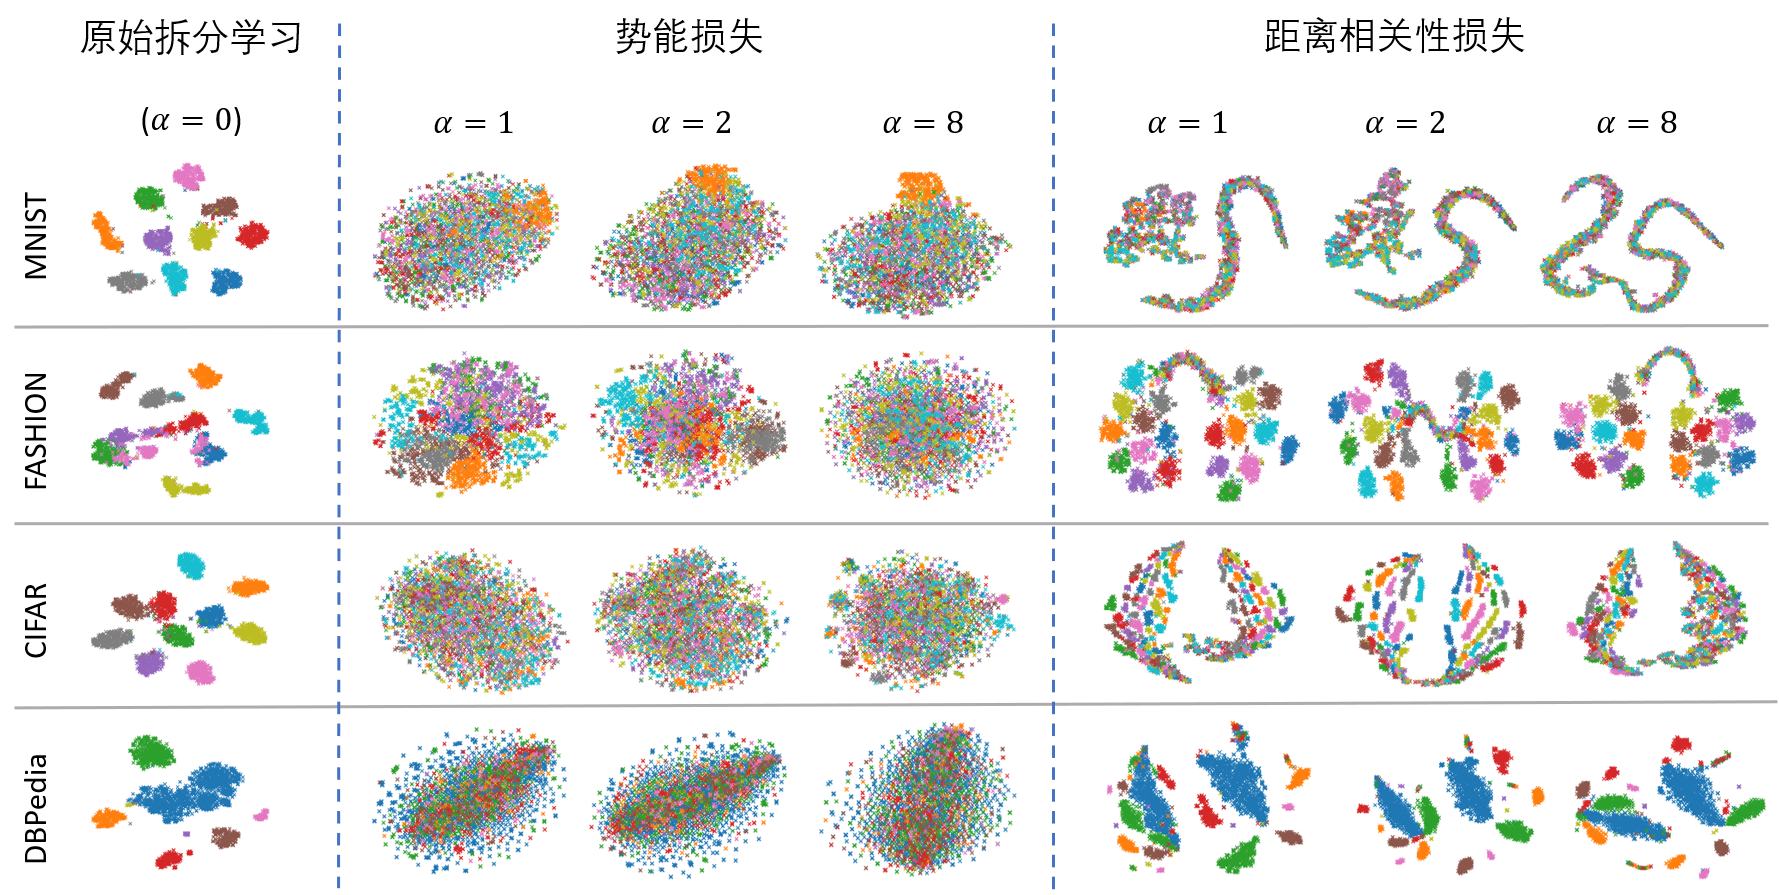
\includegraphics[width=1\linewidth]{Z_Resources/peloss_tsne}
    \caption{势能损失和距离相关性损失的隐层分布t-SNE降维}
    \label{fig:peloss:tsne}
\end{figure}


\subsection{在Transformer架构模型上的补充实验}
\begin{figure}[h!]
    \centering
    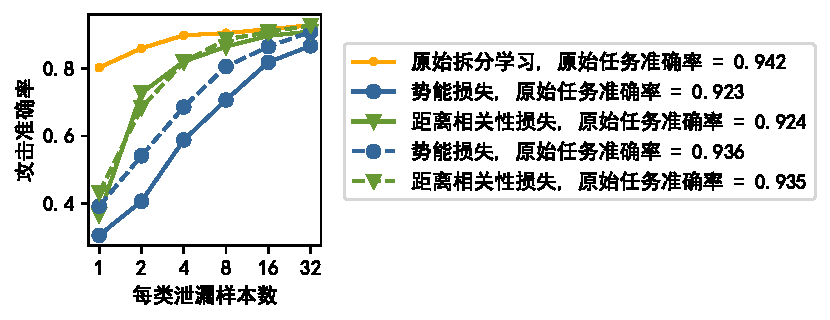
\includegraphics[width=1\linewidth]{Z_Resources/peloss_vegetable-primary}
    \caption{Vegetable Images数据集下不同泄露样本数和攻击准确率的对比}
    \label{fig:peloss:vegetable}
\end{figure}
为了进一步验证势能损失在Transformer结构的模型上的效果,我们在蔬菜图像~\cite{vegetable_2021}数据集上使用视觉Transformer(ViT, Vision Transformer)模型~\cite{alexey_2021_vit}进行了部分实验。
%
蔬菜图像数据集包含21000张图片,分为15个类别,其图片大小为$128\times 128 \times 3$。
%
我们将ViT模型的分块大小(Patch Size)设置为$16\times 16$,隐层大小为256,层数为4,注意力头(Attention Heads)个数为8。
%
实验结果呈现在\autoref{fig:peloss:vegetable}中,可以看出,势能损失在ViT模型上依然显著领先于对比的距离相关性损失。
\section{本章小结}
本章节针对拆分学习模型推断过程中的标签隐私泄露以及模型补全攻击问题,提出了受物理学现象启发的势能损失函数。
%
我们将模型补全攻击转化成一个攻击者的有监督或无监督的学习问题,通过分析泛化误差、聚类误差,表明拆分层表征分布在决策区域边缘可以增加攻击者的攻击难度,而势能损失函数恰好可以帮助样本的拆分层表征产生如此分布。
%
实验结果表明,势能损失函数在多个数据集、不同的泄漏标签数量上均优于对比算法,同时保证了原始任务准确率和攻击误差。
%
总之,势能损失降低了拆分学习推断过程中的隐私泄露问题,为拆分学习模型的实际应用提供了有力保护。
    \chapter{基于秘密分享和随机排列的高效隐私保护机器学习}
基于密码学隐私保护机器学习框架面临着非线性激活函数开销大的问题,而拆分学习和其他混合方法往往面临着中间结果产生的隐私泄漏问题。
%
为此,本文混合秘密分享技术和随机排列技术,使用秘密分享协议计算矩阵乘法灯线性运算,同时基于随机排列进行逐元素的非线性激活函数计算,提出了高效易用的隐私保护神经网络框架。
%
本文也对随机排列后的中间结果的隐私泄露程度进行了量化分析,表明随机排列可以有效地保护数据隐私。
%


\label{chap:ss-perm}
\section{研究背景}
随着机器学习在各个领域的广泛应用,数据隐私问题日益严重。
%
训练机器学习模型所需的数据可能分散在多个参与方中,比如两家医院分别有患者的CT图像数据和患者的心电图数据;银行和电商平台分别有用户的金融数据和消费数据。
%
直接把数据汇聚到一个服务器上进行中心化的模型训练,会直接暴露参与方的数据隐私。
%
类似地,在机器学习模型的部署应用阶段,用户需要将数据发送给服务器来获得模型的预测结果,这也暴露了用户的隐私数据。

%
为了解决隐私问题,许多隐私保护机器学习的方案被提出。
%
比如(横向)联邦学习(Federated Learning)~\cite{yangqiang2019federated,mcmahan_2017_fedavg}通过各方训练本地模型再聚合的方式,保护各方本地数据不出域。
但是其仅支持数据横向分割(各个参与方有不同的训练样本,但是样本的特征列是相同的)的情况,且在联邦学习过程中,模型的参数信息也会被暴露给各个参与方。
%
此外,联邦学习主要针对模型训练场景,无法在模型推断阶段提供隐私保护。
%
对于更加复杂的数据纵向分割(各个参与方有同样的样本,但是特征列不同)的情况,或是用户使用模型对自身的输入进行推断的情形,传统的横向联邦学习就无法被应用。
%
拆分学习技术~\cite{vepakomma2018split}可以适用于数据纵向分割或是模型推断的场景。
但是由于在拆分学习的训练和推断过程中,各方需要交换中间结果,因此存在较大的隐私泄漏风险,带来了诸多安全性质疑~\cite{abuadbba2020can_split,hezecheng_2019_model_inversion_attack}。
尽管第\ref{chap:randomized_topk}、\ref{chap:peloss}章提出的方案一定程度上缓解了拆分学习的隐私泄露问题,但是拆分学习交换中间结果的特性注定其无法做到对数据或模型隐私的完全保护,因此在某些安全性要求较高的领域难以应用。

为了实现计算过程中完全的、可证明的隐私保护,必须采用密码学的安全计算技术。
%
近年来,许多基于密码学的隐私保护机器学习框架被提出~\cite{mohassel2017secureml,wagh2019securenn,mohassel2018aby3}。
%
这些框架一般假设有2方或3方参与隐私保护的机器学习计算,采用秘密分享、同态加密、混淆电路等密码学基础技术,来实现安全的神经网络的推断和训练。
%
尽管基于密码学的隐私保护机器学习框架拥有可证明的安全性,其也存在着严重的效率问题。
相比于中心化的明文计算,密码学方法的通信和计算开销往往高出几个数量级。
%
由于使用密码学方法进行算术运算(加法、乘法)的技术已经相对成熟,密码学方法的性能瓶颈往往在于神经网络中的激活函数。
%
神经网络中的激活函数是非线性的,其无法用算术运算简单表示,因此需要使用开销相对较高的混淆电路协议~\cite{yao1986gc}、GMW协议~\cite{gmw_1987}或是其他的定制化协议进行安全计算,并以分段线性~\cite{mohassel2017secureml}或多项式~\cite{gilad2016cryptonets}等方法对非线性函数进行拟合。
%
另一方面,近年来也有一些研究通过将密码学与其他方法结合,设计更加高效的隐私保护机器学习框架~\cite{zhangqiao_2018_gelu_net,xiepeichen_2019_bayhenn,zhou_2022_codesign}。
%
但是这些研究一般采用了类似拆分学习的思想,部分暴露了中间结果的信息,因此存在一定程度的数据或模型的隐私泄露~\cite{wong_2020_lwe_model,abuadbba2020can_split,hezecheng_2019_model_inversion_attack}。
%
因此,如何更好地将密码学方法与非密码学方法结合以提高效率,同时尽可能地保持安全性,成为了隐私保护机器学习中亟待解决的问题。

\section{问题描述}
本节我们先探究暴露模型中间结果带来的隐私泄露问题,然后定义本章所解决的三方协作的隐私保护机器学习问题。

\subsection{隐层表征的隐私泄露}
在拆分学习或部分密码学和拆分学习等其他方法混合的隐私保护机器学习框架中,模型的部分隐层表征会暴露~\cite{zhangqiao_2018_gelu_net,vepakomma2018split,fu2022blindfl,zhou_2022_codesign}。
%
这些研究对于安全性的论证往往基于中间表征的不可逆性质,也就是在没有辅助信息的情况下,从拆分表征恢复出原始的输入特征是不可能的。
%
比如考虑全连接神经网络的第一层表征$\bvec h=W \bvec x$,其中$W \in \mathbb R^{d_1 \times d_0}$是第一层的权重(这里忽略偏置项),$X \in \mathbb R^{d_0}$表示输入表征。
%
即使攻击者收集到了大量隐层表征$H = (\bvec h_1, \cdots, h_n)$,只需要隐层表征维度$d_1$小于输入特征维度$d_0$,线性方程组
\begin{equation}
\begin{cases}
    \bvec h_1 = W \bvec x_1 \\
    \cdots \\
    \bvec h_n = W \bvec x_n \\
\end{cases}
\end{equation}
就是有无穷多解的。
%
这是因为其已知量的个数 $nd_1$ 小于未知量的个数 $d_0d_1 + nd_0$。
%
尽管一些研究在特定条件下提出了对隐层表征进行攻击从而恢复训练特征的办法,但是这些方法往往需要一些额外信息,比如底部模型权重$W$,或是部分泄露的样本-表征对$(\bvec x_i, \bvec h_i)$。
%
接下来我们将说明,即使攻击者只搜集隐层表征,而没有模型的额外信息,依然存在隐私泄露的问题。

\textbf{样本间距离信息的隐私泄露}:
%
Johnson-Lindenstrauss引理~\cite{matouvsek_2008_jl_lemma}告诉我们,对高维数据点的低维线性投影可以很大程度上保留数据点之间的距离关系。
%
也就是说,
\begin{equation}
    \Vert W \bvec x_1 - W \bvec x_2 \Vert \approx c\Vert \bvec x_1 - \bvec x_2 \Vert,    
\end{equation}
其中$c$是一个和$W$的分布以及维度相关的常数。
%
考虑到神经网络的全连接层也可以视为一个随机线性投影,因此隐层表征之间的距离也可以反应原始输入特征之间的距离,从而使得整个数据集的拓扑结构信息被暴露。
%
以MNIST数据集~\cite{mnist}为例,我们将784维的输入图片通过一个按照正态分布随机初始化的矩阵(类似于神经网络的权重初始化)投影到128维,然后对低维投影计算欧氏距离,找到最相似的样本,结果呈现在\autoref{fig:ss-perm:mnist-knn}中。
%
%
\begin{figure}[h!]
    \centering
    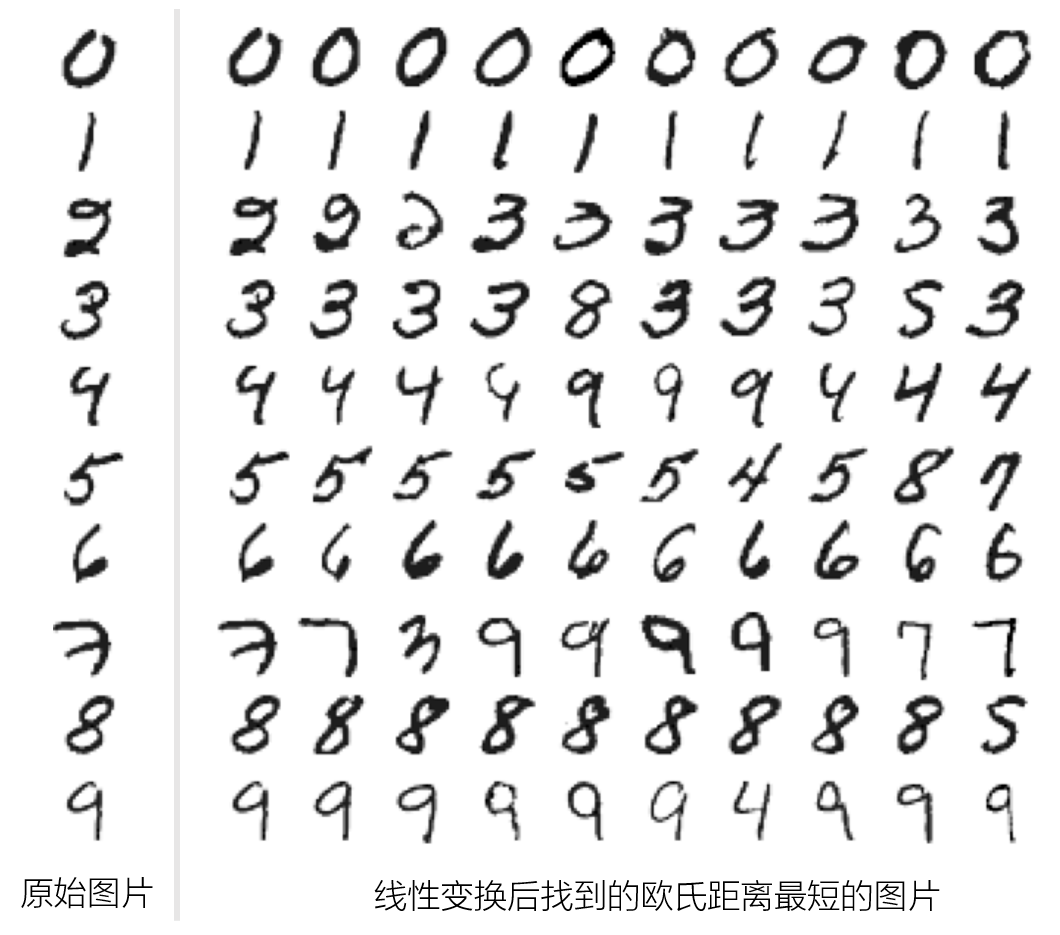
\includegraphics[width=0.66\linewidth]{Z_Resources/ss-perm_mnist-knn}
    \caption{通过对比低维投影得到的最相似样本}
    \label{fig:ss-perm:mnist-knn}
\end{figure}
%
可以看出,低维的投影相似的图片,其原始图片也十分相似。
%
因此,攻击者可以通过分析隐层表征,得到特征拥有方的数据分布、数据之间的关系,乃至数据分布随着时间变化的变化等信息。
%
以疫情防控期间的口罩检测为例,假设某公司A采用了某公司B的“口罩检测”模型来判断员工是否按照规定佩戴了口罩,并采用拆分学习(或其他需要发送隐层表征给公司B的方式)在公司内部监控摄像头的控制中心进行了模型部署。
%
公司B可以仅仅通过分析隐层表征,而无需其他任何复杂的攻击操作,来判断公司A的员工出现情况。
若某一天公司A传输的隐层表征与之前的隐层表征的相似度降低,则可以判断公司A出现了较大的人事变动情况。
%
这显然对公司A的隐私信息造成了严重泄露。


\textbf{隐层表征的重用攻击}:
在纵向联邦学习开始前,各参与方需要进行样本对齐操作,即按照统一的样本ID对各参与方数据库中的样本进行统一,保证在训练中各方采用的是相同的样本。
%
因此,在纵向联邦学习过程中,某一个恶意的参与方也可以将样本的隐层表征信息记录下来,并对这些进行滥用。
%
比如某电商公司A为了训练更好的推荐系统,与某社交平台B达成协议,让社交平台B提供一部分用户数据并且以纵向联邦的方式进行训练。
两者采用用户的手机号作为ID进行样本对齐。
%
在训练过程中,A公司可以存储隐层表征信息。
%
训练完成后,A公司可以将这些隐层表征信息,连同对应的手机号售卖给其他公司。
%
虽然这些隐层表征信息主要是通过B公司的数据以及底部模型产生的,但是在拆分学习的场景下,B公司缺少有效的技术手段检测或防止A公司对其滥用的行为。
%
因此,这种隐层表征的重复利用攻击也对拆分学习的安全性带来了不利影响。

综上所述,使用拆分学习或是其他暴露中间结果的隐私保护机器学习方法,必然要面对中间结果的隐私泄漏问题以及中间结果可能被再次利用的问题。


\subsection{问题定义}
本文考虑如下的隐私保护机器学习问题。
两方$P_0, P_1$分别持有部分数据$X$和模型参数$\Theta$,并且要进行模型的推断或训练,具体如下:
\begin{enumerate}[label=(\arabic*)]
    \item 模型推断:计算 $Y = f(X; \Theta)$,其中$f$表示模型的推断函数,是公开的。要求在推断过程中,模型参数$\Theta$和各方数据$X$,以及其他中间结果尽可能不暴露。
    模型预测值$Y$只暴露给设定的结果获取方,可能是$P_0$或$P_1$,也可以是其他方。
    \item 模型训练:计算 $\Theta' = g(X; \Theta)$,其中$g$表示模型的训练函数,其输出为更新后的参数。
    比如对于梯度下降法,$g(X;\Theta) = \Theta - \alpha \partial L(X;\Theta) / \partial \Theta$,其中$L$表示损失函数,$\alpha$是学习率。
    要求在训练过程中,模型参数$\Theta, \Theta'$,各方数据$X$,以及其他中间结果尽可能不暴露。
\end{enumerate}

在上述的隐私保护机器学习过程中,我们新增一个第三方$P_2$,其自身不带任何模型参数或数据,仅为$P_0$和$P_1$的计算提供辅助作用。
此外,我们假设各个参与方在执行特定的算法(协议)时,会遵守协议进行计算,但是可能地利用其在执行协议中接收到的信息来获取其他参与方的隐私数据。
同时,任何参与方之间不会通过共谋(Collusion)来获取其他参与方的数据。
%
这个设定在密码学中被称为半可信安全性(Semi-Honest Security)设定或诚实但好奇(Honest-but-Curious)设定,在许多隐私保护机器学习算法的设计中被采用~\cite{wagh2019securenn,mohassel2018aby3,riazi_2018_chameleon}。
\section{方法描述}
本节我们描述实现隐私保护神经网络运算的方法,包括了线性计算和非线性计算两个部分。
%
我们用$\langle \cdot \rangle$表示秘密分享状态下的数值,$\langle x \rangle_i$ 表示 $P_i$所拥有的$x$的分享值,$\pi$表示排列函数。
%
我们用$UV = W$表示秘密分享采用的Beaver三元组,用于计算$XY = Z$。
%

\subsection{基于秘密分享的线性运算}
由于本章的设定是两方拥有数据和模型,外加第三方辅助计算,因此本章采用两方加法分享(Additive Sharing)作为秘密分享方案。
%
秘密分享一般在有限域上进行,在本章中我们将其定义在整数环$\mathbb Z_N$上。
%
$\mathbb Z_N$表示模$N$的整数环,其元素为$\{0, 1, \cdots, N - 1\}$。
所有的计算都通过模$N$进行,也就是将自然数运算的结果对$N$取余数。
%
在$\mathbb  Z_N$上两方加法分享的基本运算如下:
\begin{itemize}
    \item $\mathsf{Share}(x)$:
    将一个数$x \in \mathbb Z_N$分享给$P_0$和$P_1$。
    具体而言,分享方(可以是$P_0, P_1$或其他外部参与方)产生随机数$r \stackrel{\$}{\gets} \mathbb Z_N$($\stackrel{\$}{\gets}$表示等概率地从集合中选取),然后将$\langle x \rangle_0 := r$发送给$P_0$,将$\langle x \rangle_1 := x - r$发送给 $P_1$。
    我们用$\langle  x \rangle$表示$x$处于分享状态。

    \item $\mathsf{Reconst}(\langle x \rangle, P_i)$:
    将分享状态的$\langle x \rangle$恢复给$P_i$方(默认$P_i$为$P_0,P_1$双方)。
    $P_0$和$P_1$分别把$\langle x \rangle_0, \langle x \rangle_1$发送给$P_i$,然后$P_i$计算$x = \langle x \rangle_0 + \langle x \rangle_1$。

    \item $\mathsf{Add}(\langle x \rangle, y)$:
    将一个分享状态的数$\langle x \rangle$与一个公开的数$y$相加。
    将其和记为$\langle z \rangle$,$P_0$本地计算$\langle z \rangle_0 = \langle x \rangle_0 + y$,$P_1$本地计算$\langle z \rangle_1 = \langle x \rangle_1$。
    
    \item $\mathsf{Add}(\langle x \rangle, \langle x \rangle)$:
    将两个分享状态的数$\langle x \rangle, \langle y \rangle$相加。
    将其和记为$\langle z \rangle$,$P_{i\in \{0, 1\}}$本地计算$\langle z\rangle_i = \langle x \rangle_i + \langle y \rangle_i$。
    
    \item $\mathsf{Mul}(\langle x \rangle, y)$:
    将一个分享状态的数$\langle x \rangle$与一个公开的数$y$相乘。
    将其乘积记为$\langle z \rangle$,$P_{i\in \{0, 1\}}$本地计算$\langle z\rangle_i = \langle x \rangle_i y$。

    \item $\mathsf{Mul}(\langle x \rangle, \langle y \rangle)$:
    将两个分享状态的数$\langle x \rangle, \langle y \rangle$相乘。
    该过程较为复杂,需要借助Beaver三元组才可以进行。
    本章使用辅助第三方$P_2$来产生Beaver三元组。
    %
    具体步骤如下:
    \begin{enumerate}
        \item $P_2$产生$u, v\stackrel{\$}{\gets} \mathbb Z_N$,并计算$w = uv$。
        
        \item $P_2$执行$\mathsf{Share}(u), \mathsf{Share}(v), \mathsf{Share}(w)$,将$u, v, w$分享给$P_0, P_1$。
        
        \item $P_0$和$P_1$执行$\mathsf{Reconst}(\langle x \rangle - \langle u \rangle), \mathsf{Reconst}(\langle y \rangle - \langle v \rangle)$。

        \item $P_0$计算$\langle  z \rangle_0 = (x - u)(y - v) + (x - u)\langle v \rangle_0 + \langle u \rangle_0 (y - v) + \langle w \rangle_0$;$P_1$计算$\langle  z \rangle_1 = (x - u)\langle v \rangle_1 + \langle u \rangle_1 (y - v) + \langle w \rangle_1$。
    \end{enumerate}
    我们可以简单地验证 $z = xy$。
\end{itemize}

可以看到,秘密分享的所有运算中,仅有两个分享状态的数的乘法需要参与方之间进行信息传输。
%
且对于任何一个参与方$P_i$,如果其没有关于$x$的信息,则$x - u$对其来说是一个均匀分布的随机变量;同理,如果没有关于$y$的信息,则$y - v$ 对其来说也是一个均匀分布的随机变量。
%
因此,使用上述方法计算两个分享状态的数的乘法并不会暴露任何隐私信息。
%
事实上,上述秘密分享的运算均满足信息论安全性(Information-Theoretic Security),也就是在各个参与方不共谋的情况下,即使攻击者拥有无穷的计算力,他依然无法获得任何原始数据的信息\cite{beaver1992efficient}。

尽管上述的秘密分享运算只定义在单独一个整数上,很容易可以看出我们也可以将其定义到任何向量、矩阵,乃至张量(Tensor)的运算上,乘法也可以拓展为矩阵乘法、张量乘法等一切满足乘法分配律的运算,且安全性得到完全保留。

\subsubsection{定点数编码}
一般的神经网络的计算都定义在实数上,并且以浮点数的格式进行实际的计算。
%
但是上述的秘密分享运算只适用于整数。
%
因此,我们需要定义实数与浮点数点相互转换机制。
%
我们把整数环$\mathbb Z_N$分为两个部分:$[0, \lfloor N/2 \rfloor)$ 用于表示正数,而$[\lfloor N/2 \rfloor, N)$用于表示负数。
%
对于一个实数$x$,我们首先计算其正整数部分$\lfloor x\cdot P \rceil$,其中$P$表示放缩系数(Scaling Factor),用于控制小数部分的精度。
%
然后对于负数,我们则用$N - 1$对其进行相减,得到 $N - \lfloor x\cdot P \rceil$。
%
综上所述,将实数编码为整数的函数为:
\begin{equation}
    x_Z := \mathsf{Encode}(x) = x \cdot P \bmod N.
\end{equation}
%
相应的解码函数为:
\begin{equation}
    x := \mathsf{Decode}(x_Z) = \begin{cases}
        x_Z / P         & \text{如果 $x < N/2$ ($x$是正数)}, \\
        (N - x_Z) / P     & \text{否则 ($x$ 是负数)}.
    \end{cases}
\end{equation}
%
同时,为了保证编码和解码的准确性,实数$x$必须处于区间$\big[ -\dfrac{N}{2P}, \dfrac{N}{2P} \big)$中。


\subsubsection{乘法截断}
当两个被编码的实数$x_Z, y_Z$进行乘法后,其乘积的放缩系数也是各自放缩系数的乘积:
\begin{equation}
    x_Zy_Z = (xP \bmod N)(yP \bmod N) = xyP^2 \bmod N = [(xy)_F \bmod N \cdot P] \bmod N.
\end{equation}
%
若乘法执行了$L$次,则对应的放缩系数会变为$P^L$,此时乘积是$xyP^L$,很可能已经超出了$[-N/2, N/2)$这一个有效的解码范围,导致解码错误。
%
为此,我们需要在每次乘法之后进行截断操作,即
\begin{equation}
    z = xy \Rightarrow z_Z = \Big\lfloor \dfrac{(x_Z y_Z) \bmod P}{P} \Big\rceil.
\end{equation}
%

在明文状态下,该截断操作可以直接执行。
%
对于秘密分享状态下的正整数,则截断操作会更为复杂。
%
SecureML~\cite{mohassel2017secureml}论文的作者采用了两方直接本地截断(Local Truncation)的办法,也就是:
\begin{equation}
    \langle z_Z \rangle_i \gets \langle x_Zy_Z \rangle_i / P.
\end{equation}
%
注意这里的除法需要考虑符号位。
此处我们直接用“/”来表示整数除法($\lfloor \cdot / \cdot \rceil$)。
%
可以证明,该方法能够以很大的概率产生和在明文上截断最多相差1的结果。

\begin{theorem}[本地截断]
\label{thm:ss-perm:local-truncation}
    对于在$\mathbb Z_N$下分享状态的数$\langle x \rangle_0, \langle x \rangle_1$,且$|x| \le x_\text{max} < N/2$,则最多有
    $\dfrac{2x_\text{max}}{N}$的概率使得$\langle x \rangle_0/P + \langle x \rangle_1/P\notin [x/P - 1, x/P + 1]$。
\end{theorem}
\begin{proof}
    首先考虑$\langle x \rangle_0, \langle x \rangle_1$符号相反的情况,此时在$\mathbb Z$上有$\langle x \rangle_0 + \langle x \rangle_1 = x$。
    注意到因为四舍五入的误差不超过0.5,因此对于任何$a + b = c \in \mathbb R$,有$\lfloor a \rceil + \lfloor b \rceil \in [\lfloor c \rceil - 1, \lfloor c \rceil + 1]$。
    将其带入$\langle x \rangle_0/P + \langle x \rangle_1/P = x/P$,即可得到$\langle x \rangle_0, \langle x \rangle_1$符号相反时该结论成立。
    接下来考虑$\langle x \rangle_0, \langle x \rangle_1$符号相同的概率。
    %
    假设$-x_\text{max} \le x \le 0$,则需要满足 
    %
    \begin{equation}
    \begin{cases}
        0 \le \langle x \rangle_0 < N/2, \\
        0 \le x - \langle x \rangle_0 < N/2.
    \end{cases}
    \end{equation}
    第二行可以改为$N/2 < \langle x \rangle_0 - x \le N$,只有$\langle x \rangle_0 \in (N/2 + x, N/2)$时,上述条件成立。
    再考虑$-x_\text{max} \le x \le 0$,得到其概率小于 $2x_\text{max}/N$。
    对于$0 \le x \le x_\text{max}$的情况,我们也可以得到类似结果$\langle x \rangle_0 \in [N/2, N/2 + x)$,证明完毕。
\end{proof}
%
上述定理表明,采用简单的本地截断方法,其截断出错的概率也是很小的。
%
但是小概率的截断错误在神经网络训练中也是不可接受的,下面我们举例说明。
%
比如我们令$N = 2^{64}$,放缩系数$P = 2^{20}$,$|x|, |y| \le 2^{8}$,则经过一次乘法$z = xy$,$|z| \le 2^{56}$。
%
通过\autoref{thm:ss-perm:local-truncation}可以得到,此时截断出错的概率小于$2 \times 2^{56} / 2^{64} = 1/128$。
%
考虑到神经网络的计算中会涉及到较大的矩阵,则截断出错很容易在计算中出现。
%
不仅如此,我们可以看到该截断产生的误差是非常大的,可以到接近$\dfrac{N}{2P}$的量级。
%
如此巨大的误差将会给神经网络的训练或推断带来重大的影响,使得其结果毫无意义。
%
因此,我们必须采取措施避免简单的“本地截断”带来的误差。


根据\autoref{thm:ss-perm:local-truncation}的分析,可以看到截断错误是否发生与$\langle x \rangle_0$有关。
%
具体而言,当$|\langle x \rangle_0| \in (N/2-x_\text{max}, N/2]$时,才有可能产生截断错误。
%
因此,对$x$进行截断时,我们只需要让$P_0$检查$|\langle x \rangle_0|$是否在可能截断错误的范围内,再对其进行缩小处理。如果$|\langle x \rangle_0|$在该范围内,若$\langle x\rangle_0$为正数(在$[0, N/2)$区间),则$P_0$首先计算$\langle x \rangle_0 \gets \langle x \rangle_0 - N/4$,并发送“+”给$P_1$,$P_1$执行$\langle x \rangle_1 \gets \langle x \rangle_1 + N/4$。
%
注意到这种方法会暴露关于$x$的范围信息,但是其暴露的概率较小(等价于定理\autoref{thm:ss-perm:local-truncation}中截断出错的概率),且即使暴露,很大概率也只暴露一个宽度为$x_\text{max}$左右的范围。
%
考虑到神经网络的计算过程中的变量元素都很多,暴露其中很少部分元素的范围不会造成实质性的隐私泄露。
%
总而言之,本章所以出的方法是将小概率的截断错误转化为小概率的部分元素范围泄露。
因为在神经网络的训练和推断中往往涉及到数量庞大的大规模的矩阵运算,即使是小概率的截断错误,由于其错误的误差极大,也会导致神经网络的训练崩溃或输出无意义结果。
而相比之下,泄露少量元素的范围并不会让攻击者窃取有意义的隐私数据。
%
因此,本章提出的截断方法更适合神经网络的安全计算。

\subsubsection{优化的秘密分享乘法}
为了进一步提高效率,我们注意到上述截断过程可以与秘密分享的乘法过程绑定,从而实现减少通信量的目的。
%
在秘密分享的乘法中,$P_0$和$P_1$之间要进行两次通信来重构$x - u$和$y - v$,分别是$P_0$发送自身对应的分享值和$P_1$发送自身对应的分享值。
%
假设$P_1$先发送自身的秘密分享值,则$P_0$收到分享值后,可以先计算乘积分享值$\langle z \rangle_0$,同时利用该值检查是否有需要进行缩小,再把是否需要缩小的信息连同$\langle x \rangle_0 - \langle u \rangle_0, \langle y \rangle_0 - \langle v \rangle_0$一同发给$P_1$。
%
这样不会在秘密分析乘法中带来任何额外的通信。
%
我们将优化后的秘密分享张量乘法定义在\autoref{alg:ss-perm:ss-mul}中。


\begin{algorithm}[h!]
\caption{秘密分享乘法$\mathsf{SSMul}$}
\label{alg:ss-perm:ss-mul}
    \begin{algorithmic}[1]
    \Require{秘密分享的张量$\langle X \rangle, \langle Y \rangle$;乘法函数$f_\text{mul}$;放缩系数$P$;结果范围$z_\text{max}$}
    \Ensure{秘密分享的张量$\langle Z = \dfrac{XY}P \rangle$}
    \State 各方将默认乘法设置为$f_\text{mul}$ \LineComment{视具体情况,可以是逐元素乘法、矩阵乘法等}
    \State $P_2$生成Beaver三元组$UV=W$($U, V$形状和$X, Y$相同,其元素从$\mathbb Z_N$中均匀采样),并将其秘密分享给$P_0, P_1$
    \State $P_1$发送$\langle X \rangle_1 - \langle U \rangle_1, \langle Y \rangle_1 - \langle V \rangle_1$给$P_0$
    %
    \State $P_0$恢复出
    $X - U = \langle X \rangle_0 - \langle U \rangle_0 + \langle X \rangle_1 - \langle U \rangle_1, 
     Y - V = \langle Y \rangle_0 - \langle V \rangle_0 + \langle Y \rangle_1 - \langle V \rangle_1$
    %
     \State $P_0$计算出$\langle Z \rangle_0 = (X - U)(Y - V) + (X - U)\langle V \rangle_0 + \langle U \rangle_0 (Y - V) + \langle W \rangle_0$
    %
    \State $P_0$找出$\langle Z \rangle_0$中满足 $\langle Z \rangle_0[i] \in (N/2 - z_\text{max}, N/2)$的下标$i$集合,记作$I_\text{large}$;同理找到$\langle Z \rangle_0[i] \in [-N/2, -N/2 + z_\text{max})$的下标$i$集合,记作$I_\text{small}$
    %
    \NewlineComment{此处下标为把张量$\langle Z \rangle_0$转化为1维向量的下标}
    %
    \For{$i \in I_\text{large}$}
        \State $P_0$ 更新 $\langle Z \rangle_0[i] \gets \langle Z \rangle_0[i] - N/4$
    \EndFor
    \For{$i \in I_\text{small}$}
        \State $P_0$ 更新 $\langle Z \rangle_0[i] \gets \langle Z \rangle_0[i] + N/4$
    \EndFor
    %
    \State $P_0$发送$\langle X \rangle_0 - \langle U \rangle_0, \langle Y \rangle_0 - \langle V \rangle_0, I_\text{small}, I_\text{large}$给$P_1$
    %
    \State $P_1$恢复出$X - U, Y - V$
    \State $P_1$计算出$\langle Z \rangle_1 = (X - U)\langle V \rangle_1 + \langle U \rangle_1(Y - V) + \langle W \rangle_1$
    %
    \For{$i \in I_\text{large}$}
        \State $P_1$ 更新 $\langle Z \rangle_1[i] \gets \langle Z \rangle_1[i] + N/4$
    \EndFor
    \For{$i \in I_\text{small}$}
        \State $P_1$ 更新 $\langle Z \rangle_1[i] \gets \langle Z \rangle_1[i] - N/4$
    \EndFor
    \end{algorithmic}
\end{algorithm}




\subsection{基于随机排列的激活函数计算}
神经网络中除了矩阵的线性运算(加法、乘法),另一种不可或缺的运算是非线性激活函数(Activation Function)。
%
若没有激活函数,则整个神经网络将退化为一个线性映射。
%
由于激活函数是非线性的,甚至无法使用多项式表示,因此其对密码学方案不友好,当前许多研究采用混淆电路或其他精心设计的MPC协议计算,产生了大量的开销,同时由于其中采用了近似计算,可能还会带来神经网络的精确度损失~\cite{mohassel2017secureml,liujian2017minionn,mishra2020delphi}。
%
另一方面,如果将神经网络中间结果发送给第三方来算激活函数,则第三方可以根据中间结果来反推神经网络的权重。
%
为此,本章提出利用随机排列来安全地解决激活函数的计算。


对$n$个元素进行随机排列(Random Permutation),表示将$n$个元素打乱顺序,总共有$n!$种不同的排列顺序。
%
注意到,排列的数目随着$n$的增长呈现出超指数(Super-Exponential)增长,因此即使是较少的元素,其可能的排列顺序也是天文数字。
%
比如,仅仅10个元素有360多万种排列($\approx 2^{22}$);而当元素个数增长到100,则可能的排列数超出$2^{524}$。
%
如此大量的排列个数,使得从随机排列中猜测出原排列的概率几乎为0。
%
考虑到神经网络中间结果往往是包含大量元素的张量,我们可以认为对其进行随机排列后几乎可以消除所有原始张量的信息。
%
并且注意到,神经网络的激活函数是作用于每个元素上的(Element-Wise),因此打乱顺序后执行激活函数与执行激活函数后再打乱顺序是等价的。

因此,我们可以让$P_0$和$P_1$对秘密分享的神经网络中间结果执行随机排列后,再恢复到$P_2$上。
%
$P_2$随即在随机排列后的明文上计算出激活函数的值,再将其重新分享给$P_0$和$P_1$两方。
%
$P_0$和$P_1$可以通过逆向排列,恢复出最终结果的分享值。
%
注意到,在此过程中,$P_0$和$P_1$必须采用同样的随机排列,否则会导致恢复错误。
%
此外,我们还可以通过(在元素数量不足够大时)添加扰动元素;对Tanh、Sigmoid等对称激活函数在随机排列中加入随机翻转来进一步提高安全性。
上述方法实现简单,本文不再赘述。
%
我们将该方法在\autoref{alg:ss-perm:perm-act}中进行具体描述。


\begin{algorithm}[h!]
    \caption{基于随机排列的激活函数计算方法$\mathsf{PermNonlinear}$}
    \label{alg:ss-perm:perm-act}
        \begin{algorithmic}[1]
        \Require{秘密分享的张量$\langle X \rangle$;激活函数$f$}
        \Ensure{秘密分享的张量$\langle Y = f(X) \rangle$}
        %
        \State $P_0$ 生成一个随机排列 $\pi \stackrel{\$}{\gets} \text{Perm}(\text{Size}(X))$
        \LineComment{Size$(X)$表示张量$X$的元素个数}
        \State $P_0$ 将$\pi$ 发送给$P_1$
        %
        \State $P_0, P_1$分别将$\pi[\langle X \rangle_0], \pi[\langle X \rangle_1]$发送给$P_2$
        %
        \State $P_2$恢复出$\pi[X] = \pi[\langle X \rangle_0] + \pi[\langle X \rangle_1]$,并计算出$\pi[f(X)] = f(\pi[X])$
        \State $P_2$将$\pi[f(X)]$分享给$P_0, P_1$
        \State $P_0$和$P_1$分别计算得到$\langle Y \rangle_0 = \pi^{-1} \langle \pi[f(X)] \rangle_0, \langle Y \rangle_1 = \pi^{-1} \langle \pi[f(X)] \rangle_1$
    \end{algorithmic}
\end{algorithm}


通过该方法,我们可以极大的降低激活函数的计算开销。我们在\autoref{tab:ss-perm:relu}中对本方法和对比算法的ReLU激活函数计算的通信轮次/通信量进行对比。
%
表中的$p$是一个质数(一般为三位数),$k$是混淆电路的安全性参数(Security Paramter),一般大于128。
%
注意到,本方法的开销已经考虑了下一节所用基于关联随机性(Correlated Randomness)的通信优化算法。

\begin{table}[t]
    \caption{不同算法ReLU开销对比}
    \label{tab:ss-perm:relu}
    \centering
    \begin{tabular}{ccc}
    \toprule
    算法 & 通信轮次 & 通信量(比特) \\ 
    \midrule
    本方法 & $3$ & $3L$ \\
    SecureNN\cite{wagh2019securenn} & $11$ & $8L\log_2 p + 32L + 2$ \\
    ABY3\cite{mohassel2018aby3} & $6 + \log L$ & $105L$ \\
    混淆电路\cite{rouhani2018deepsecure} & $4$ & $k(3L - 1)$ \\
    \bottomrule
    \end{tabular}
\end{table}

\subsection{基于关联随机性的通信优化}
两方具有关联随机性,可以理解为两方有一个同样的伪随机数生成器(Pseudo-Random Generator),可以使得其每次采样时产生同样的随机数。
%
通过关联随机性,我们可以进一步降低上述的秘密分享乘法(\autoref{alg:ss-perm:ss-mul})以及基于随机排列的激活函数计算方法(\autoref{alg:ss-perm:perm-act})的通信复杂度~\cite{riazi_2018_chameleon}。
%

\textbf{优化\textsf{SSMul}}:具体而言,$P_0$和$P_2$分享一个伪随机数生成器$G_\text{beaver}$。
在\autoref{alg:ss-perm:ss-mul}第2行中,$P_2$使用$G_\text{beaver}$产生Beaver三元组给$P_0$的分享:$\langle U \rangle_0, \langle V \rangle_0, \langle W \rangle_0 \gets G_\text{beaver}$。
同时,$P_0$自身也可以产生这些分享,因此$P_2$无需再将这些分享值发送给$P_0$。


\textbf{优化\textsf{PermNonlinear}}:$P_0$和$P_1$分享一个伪随机数生成器$G_\text{perm}$,用于在\autoref{alg:ss-perm:perm-act}中产生同样的随机排列。因此,\autoref{alg:ss-perm:perm-act}第2行可以改为$P_1$通过$G_\text{perm}$产生随机排列,从而减少一次通信。
%
此外,$P_0$和$P_2$分享一个伪随机数生成器$G_\text{share}$,用于$P_2$产生$\langle \pi[f(X)] \rangle_0$时。此时在\autoref{alg:ss-perm:perm-act}第5行时,$P_2$无需再将$\langle \pi[f(X)] \rangle_0$发送给$P_0$,从而减少一次通信。


\subsection{隐私保护神经网络框架实现}
基于上述的秘密分享乘法和基于随机排列的激活函数,我们已经能够实现基本的全连接神经网络的推断和训练。
%
在神经网络中有如下的操作:
\begin{itemize}
    \item 线性运算:加法、减法、乘法(包含矩阵乘法和逐元素相乘);
    \item 激活函数运算:比如ReLU、Sigmoid、Tanh等;
    \item 本地计算:包括了矩阵转置(Transpose)等。
\end{itemize}
%
对于加法和乘法,我们采用秘密分享以及本章提出的\autoref{alg:ss-perm:ss-mul}来实现。
对于减法$x - y$,我们将其转换为$x + (-y)$,而负数在秘密分享中也只需要双方本地将该数取负号(在$\mathbb Z_N$中,$-x = N - x$)。
%
对于激活函数,采用上述的\autoref{alg:ss-perm:perm-act}实现。
%
综上,我们将全连接神经网络的推断和训练在\autoref{alg:ss-perm:train}和\autoref{alg:ss-perm:infer}中进行描述。
%
\begin{algorithm}[h!]
    \caption{隐私保护神经网络推断$\mathsf{PriavteNNInfer}$}
    \label{alg:ss-perm:train}
        \begin{algorithmic}[1]
        \Require{秘密分享的输入$\langle X \rangle$;秘密分享的第$i$层权重$\langle W \rangle_i$;偏置$\langle \bvec b \rangle_i$;激活函数$f_i$}
        \Ensure{秘密分享的神经网络输出$\langle Y\rangle$}
        %
        \State $\langle H \rangle_0 \gets \langle X \rangle$
        \For{$i = 0$ to $L -1$} \LineComment{$L$为总层数}
            \State $\langle Z_{i + 1} \rangle = \mathsf{SSMul}(\langle H_i \rangle, \langle W_i \rangle^T, \text{矩阵乘}) + \langle \bvec b_i \rangle$
            \State $\langle H_{i + 1} \rangle = \mathsf{PermNonlinear}(\langle Z \rangle_{i+1}, f_i)$
        \EndFor
        \State \Return $\langle H_L\rangle$
    \end{algorithmic}
\end{algorithm}

%
\begin{algorithm}[h!]
\caption{隐私保护神经网络训练$\mathsf{PriavteNNTrainStep}$}
\label{alg:ss-perm:infer}
    \begin{algorithmic}[1]
    \Require{秘密分享的输入特征$\langle X \rangle$ 和标签$\langle Y \rangle$;秘密分享的第$i$层权重$\langle W \rangle_i$;偏置$\langle \bvec b \rangle_i$;激活函数$f_i$;学习率$\alpha$}
    \Ensure{一次梯度下降后更新的权重和偏置}
    %
    \State 各方执行$\langle Y' \rangle \gets \mathsf{PrivateNNInfer}(\langle X \rangle, (\langle W \rangle_i, \langle \bvec{b} \rangle_i, f_i))$,
        并且在执行过程中保留中间变量$\langle Z_1 \rangle, \cdots, \langle Z_L \rangle$和$\langle H_1 \rangle, \cdots, \langle H_L \rangle$
    %
    \State $\langle G_L \rangle \gets 2 \cdot (\langle Y \rangle - \langle Y' \rangle)$
    %
    \For{$i = L - 1$ to $0$} \LineComment{$L$为总层数}
        \State $\langle G'_{i + 1} \rangle \gets \mathsf{PermNonlinear}(\langle Z_{i+1} \rangle, \dfrac{df_i}{dx})$ \LineComment{$\dfrac{df_i}{dx}$也是逐元素函数}
        \State $\langle G_{i + 1} \rangle \gets \mathsf{SSMul}(\langle G'_{i+1} \rangle, \langle G_{i+1} \rangle, \text{元素乘})$
        \State $\langle G_{i} \rangle \gets \mathsf{SSMul}(\langle G_{i+1} \rangle, \langle W_i \rangle, \text{矩阵乘})$ \LineComment{对权重进行了转置}
        \State $\langle \bvec b_i \rangle \gets \langle \bvec b_i \rangle - \alpha \cdot \mathsf{sum}(\langle G_i \rangle, \mathsf{axis}=0)$ \LineComment{\textsf{sum}可以表示为秘密分享的加法}
        \State $\langle W_i \rangle \gets \langle W_i \rangle - \alpha \cdot \mathsf{SSMul}(\langle G_i \rangle^T, \langle H_i \rangle, \text{矩阵乘})$
    \EndFor
\end{algorithmic}
\end{algorithm}

%
\section{安全性分析}
本章提出的隐私保护神经网络的线性计算部分采用秘密分享进行设计,在半可信安全性设定下满足信息论安全~\cite{demmler2015aby}。
%
因此,本节讨论基于随机排列的非线性激活函数计算的安全性。
%
尽管前文已经展示了可能的随机排列个数随着元素个数$n$的增长而超指数增长,本节采用了更加精确的量化手段基于分析。
%
具体而言,本节采用了距离相关性(Distance Correlation)作为安全性指标,对于随机排列以及简单的线性变换(拆分学习中直接暴露中间结果的情况)进行了分析,显示了随机排列带来的隐私泄露极小。

\subsection{距离相关性}
距离相关性(Distance Correlation)~\cite{szekely2007dcor,szekely2009brownian_dcor}是一种统计学上的相关性度量,可以度量任意两个高维向量之间的相关性。
相对于常用的皮尔逊相关性系数(Pearson Correlation Coefficient),距离相关性可以对任意两个不同维度的高维随机向量进行建模,并且可以捕获非线性的相关性,只有在两个随机向量完全无关时才会为0。
%
因此,距离相关性适合用来分析高维向量之间的关联性。

\begin{definition}[距离相关性]
    对于两个随机向量$X \in \mathbb R^p, Y\in \mathbb R^q$,距离相关性的定义为
    \begin{equation}
        \textnormal{DCOR}(X, Y) = \dfrac{\mathcal{V}(X, Y)^2}{\sqrt{\mathcal{V}(X, X)^2\mathcal{V}(Y, Y)^2}},
    \end{equation}
    其中$\mathcal{V}$表示距离协方差(Distance Covariance),定义如下
    \begin{equation}
        \mathcal{V}(X, Y)^2 = \dfrac{1}{c_pc_q} \int_{\mathbb R^{p + q}}
        \dfrac{|f_{X, Y}(t, s) - f_X(t)f_Y(s)|^2}{\Vert c_p \Vert^{p+1}\Vert c_q \Vert^{q+1}}dtds,
    \end{equation}
    其中,$c_p, c_q$为两个常数,$\Vert \cdot \Vert$表示欧几里得范数(Euclidean Norm)。
\end{definition}

除去上述的定义为,距离协方差还可以通过
\begin{equation}
\begin{split}
    \mathcal{V}(X, Y)^2 = 
    & \quad \mathbb E \Vert X-X'\Vert \Vert Y -Y'\Vert +\mathbb E\Vert X -X' \Vert \mathbb E \Vert Y -Y' \Vert
    \\ & 
    - \mathbb E\Vert X-X'\Vert  \Vert Y -Y''\Vert - \mathbb E \Vert X -X''\Vert  \Vert Y -Y' \Vert
\end{split}
\end{equation}
来计算,其中$(X, Y), (X', Y'), (X'', Y'')$是相互独立的。
%
通过上式可以以采样的方式来估算距离相关性。

\subsection{随机线性变换的距离相关性}
现在我们研究随机线性变换后的向量与随机变换之前的向量的距离相关性。
我们用$\angle[\cdot, \cdot]$表示两个向量之间的夹角。
\begin{theorem}
\label{thm:ss-perm:linear-dcov}
    令$X\in \mathbb R^n$是一个随机的$n$维随机向量,令$Y = AX$,
    %
    其中 $A \in \mathbb R^{n \times d}$是一个随机线性变换,并且满足在单位正交变换下概率不变,即$P(A) = P(AT)$, $T$是$n$维单位正交矩阵(Orthonormal Matrix)。
    %
    则
    \begin{equation}
    \label{eq:ss-perm:linear-dcov1}
            \mathop{\mathbb E}_A \mathcal{V}(X, AX)^2 = a\mathcal{V}(X, X)^2,
    \end{equation}
    以及    
    \begin{equation}
    \label{eq:ss-perm:linear-dcov2}
        \mathop{\mathbb E}_A \mathcal{V}(AX, AX)^2 = {a^2S_1 + b^2S_2 - 2S_3'},
    \end{equation}
    其中 $S_1 = \mathbb \Vert X - X'\Vert^2, S_2 = \left( \mathbb E \Vert X - X'\Vert \right)^2, S_3 = \mathbb E \Vert X - X' \Vert \Vert X - X'' \Vert$,\\
    $S' = \mathbb E \left[ g(\angle [X - X', X - X'']) \cdot \Vert X - X'\Vert \Vert X - X'' \Vert \right]$,
    以及
    $g_A(\theta) = \mathbb E_A \dfrac{\Vert A\bvec x \Vert \Vert A\bvec y \Vert}{\Vert \bvec x \Vert \Vert \bvec y \Vert} $,
    $a = \mathbb E_A \dfrac{\Vert A\bvec x \Vert}{\Vert \bvec x \Vert}$,
    $b = \sqrt{\mathbb E_A \dfrac{\Vert A\bvec x \Vert^2}{\Vert \bvec x \Vert^2}}$,$\bvec x, \bvec y$为任意的$n$维向量,且夹角为$\theta$。
\end{theorem}
\begin{proof}
我们用$\mathbb E$来简略表示$\mathbb E_{X,X',X''}$。
%
首先注意到$\mathbb E_A\mathbb E\Vert X - X' \Vert \Vert A(X - X') \Vert = \mathbb E \left[ \Vert X - X'\Vert^2 \mathbb E_A \dfrac{\Vert A(X - X') \Vert }{\Vert X - X'\Vert} \right]$。
%
可以看出$\mathbb E_A \dfrac{\Vert A(X - X') \Vert }{\Vert X - X'\Vert}$和$X$无关,因此可以进一步写成
$\mathbb E \Vert X - X'\Vert^2 \cdot \mathbb E_A \left[ \dfrac{\Vert A(X - X') \Vert }{\Vert X - X'\Vert} \right] = a\mathbb E \Vert X - X'\Vert^2$。
%
同理可得\autoref{eq:ss-perm:linear-dcov1}的推导。
另外
\begin{equation}
\begin{split}
    \mathbb E_A \mathbb E{\Vert AX - AX' \Vert \Vert AX - AX'' \Vert} = 
    \mathbb E \mathbb E_A \Vert A(X - X') \Vert \Vert A(X - X'') \Vert \\
    =
    \mathbb E \left[ \Vert X - X' \Vert \Vert X - X'' \Vert \mathbb E_A \dfrac{\Vert A(X - X') \Vert \Vert A(X - X'') \Vert}{\Vert X - X' \Vert \Vert X - X'' \Vert}  \right].
\end{split}
\end{equation}

下面我们证明$\mathbb E_A \dfrac{\Vert A\bvec x\Vert \Vert A \bvec y\Vert }{\Vert \bvec x \Vert \Vert \bvec y \Vert}$只和$\bvec x, \bvec y$之间的夹角有关。
%
由于对$\bvec x, \bvec y$放缩不影响结果,我们考虑两对$n$维向量$\bvec x, \bvec y$与$\bvec x', \bvec y'$满足$\Vert \bvec x \Vert = \Vert \bvec x' \Vert = \Vert \bvec y \Vert = \Vert \bvec y' \Vert = 1$,
且$\bvec x, \bvec y$和$\bvec x', \bvec y'$的夹角均为$\theta$。
%
令$\bvec e_1 = \bvec x/\Vert x \Vert, \bvec e_2 = (\bvec y - \bvec y \cdot \bvec x/\Vert \bvec x \Vert) / \Vert \bvec y - \bvec y \cdot \bvec x/\Vert \bvec x \Vert \Vert$,
且$\bvec e_3, \cdots, \bvec e_n$是与$\bvec e_1, \bvec e_2$正交的任意$n-2$组单位正交向量组。
%
此时,有$\bvec x = \bvec e_1, \bvec y = \cos \theta \bvec e_1 + \sin \theta \bvec e_2$。
%
同理,我们也可以把$\bvec x'$和$\bvec y'$表示为$\bvec e_1'$与$\cos \theta \bvec e'_1 + \sin \theta \bvec e'_2$。
%
此时$(\bvec e_1, \cdots, \bvec e_n)$与$(\bvec e'_1, \cdots, \bvec e'_n)$是$\mathbb R^n$的两组单位正交基,因此存在单位正交矩阵$T$使得$T\bvec e_i = \bvec e'_i$。
%
也就是$\dfrac{\Vert A\bvec x \Vert\Vert A\bvec y \Vert}{\Vert \bvec x\Vert \Vert \bvec y \Vert} = \dfrac{\Vert AT\bvec x' \Vert\Vert AT\bvec y' \Vert}{\Vert \bvec x'\Vert \Vert \bvec y' \Vert}$。
%
注意到$P(A)=P(AT)$,因此$\mathbb E_A f(A) = \mathbb E_A f(AT)$,令$f(A) = \dfrac{\Vert A\bvec x \Vert\Vert A\bvec y \Vert}{\Vert \bvec x\Vert \Vert \bvec y \Vert}$ 可以得到$f(A)$仅仅和$\theta$有关。
%
于是有$\mathbb E_A \mathcal{V}(AX, AX) = b^2 S_1 + a^2 S_2 - 2S_3'$,也就是\autoref{eq:ss-perm:linear-dcov2}。
\end{proof}

\autoref{thm:ss-perm:linear-dcov}显示出,当$A$是一个具有旋转不变性(Rotation Invariance)分布的随机线性变换时,$\mathcal{V}(X, AX)/\mathcal{V}(X, X)$的期望值只和$A$有关,而和$X$的具体分布无关。
%
同时,$\mathbb E_A \mathcal{V}(AX, AX)$随着$g_A(\theta)$的提升而降低。
%
我们可以进一步证明,$g_A(\theta)$在$[0, \pi/2]$上是单调递减的。
%
\begin{proposition}
    $g_A(\theta)$在$[0, \pi/2]$上是单调递减的。
\end{proposition}
%
\begin{proof}
    由于$A$的分布具有旋转不变性,不妨令
    $\bvec x = \begin{bmatrix}
        \cos \theta/2 \\ \sin \theta/2 \\ \bvec 0   
    \end{bmatrix}$
    和
    $\bvec y = \begin{bmatrix}
        \cos \theta/2 \\ \sin \theta/2 \\ \bvec 0
    \end{bmatrix}$,
    此时有 $g_A(\theta) = \mathbb E_A \Vert A\bvec x\Vert \Vert A \bvec y\Vert$。
    我们可以对$A$在前两个维度构成的平面上进行旋转角度$\alpha$:
    \begin{equation}
        AT = A \begin{bmatrix}
            \cos \alpha & \sin \alpha & O \\
            -\sin \alpha &\cos \alpha & O \\
            O & O & E
        \end{bmatrix}.
    \end{equation}
    此时有:
    \begin{equation}
    \begin{split}
        \mathbb E_A \Vert A\bvec x \Vert \Vert A \bvec y \Vert = \mathbb E_A \Vert AT \bvec x \Vert \Vert AT \bvec y \Vert = \mathbb E_A \mathbb E_T \Vert AT \bvec x \Vert \Vert AT \bvec y \Vert \\
        = \mathbb E_A \mathbb E_\alpha 
        \left[
        \Vert \cos(\alpha - \theta/2)\bvec a_0 - \sin (\alpha - \theta/2) \bvec a_1\Vert 
        \cdot
        \Vert \cos(\alpha + \theta/2)\bvec a_0 - \sin (\alpha + \theta/2) \bvec a_1\Vert
        \right],
    \end{split}   
    \end{equation}
    其中,$\bvec a_0, \bvec a_1$是$A$的前两列。
    %
    对$\theta$进行求导,得到:
    \begin{equation}
        \begin{split}
            & \dfrac{d\mathbb E_\alpha \Vert A\bvec x \Vert \Vert A\bvec y \Vert}{d\theta} = 
            -(\Vert \bvec a_0 \Vert^2 + \Vert \bvec a_1 \Vert^2)\sin \theta \cdot \\
            & \int_{\alpha=0}^{2\pi} 
                \text{Sign}[(\Vert \bvec a_0 \Vert^2 - \Vert\bvec a_1\Vert^2)\cos 2 \alpha] - 
                (\bvec a_0 \cdot \bvec a_1) \sin 2\alpha + 
                (\Vert \bvec a_0 \Vert^2 + \Vert\bvec a_1\Vert^2) \cos \theta d\alpha.
        \end{split}
    \end{equation}
    注意到积分号中的前两项积分后为0,整个式子为负数,因此我们可以得出$g(\theta)$在$[0, \pi/2]$中单调递减。
\end{proof}

直观角度理解,$S'$项反应了分布$X$的“集中度”对距离方差带来的影响。
%
当$X$中的各个点分布在很接近的方向上时,$\angle[X - X', X - X'']$变小,因此$S'$变大,从而导致$\mathcal{V}(AX, AX)$变小,随之$\text{DCOR}(X, AX)$变大。
%
也就是说,$X$的分布的方向越集中,则与其随机线性投影的距离相关性有更大可能变大。
%
在极端情况下,$X$分布在一条线上,则$S' = S_3$取得最大值。
%
同时,变换$A$若能尽可能保留数据点之间的距离,则也能提高变换前后的距离相关性。
%
如果$A$是保距变换(Distance-Preserving Transformation),则显然$\text{DCOR}(X, AX) = 1$。


%
在神经网络中,我们一般采用$\mathcal N(0, \sigma^2)$来初始化全连接权重。
%
考虑$W \sim \mathcal N(0, \sigma^2)^{n \times d}$,此时考虑对向量$\bvec e_1$计算$\mathbb E_A \Vert W\bvec e_1 \Vert$与$\sqrt{\mathbb E_A \left[\Vert W\bvec e_1 \Vert^2 \right]}$,对应卡方分布(Chi-Square Distribution)的均值以及其平方根的均值。
%
因此可以得到
$a = \mathbb E \sqrt{w_1^2 + \cdots + w_d^2} = \sigma \sqrt{2} \Gamma(d + 1/2) / \Gamma(d) \approx \sigma \sqrt{d - 1/2}$(对于较大的 $d$),
$b = \mathbb E \left[ {w_1^2 + \cdots + w_d^2} \right] = \sigma\sqrt{d}$。
%
再考虑$\bvec x = \bvec e_1, \bvec y = \cos \theta \bvec e_1 + \sin \theta \bvec e_2$,可以得到
\begin{equation}
    g_A(\theta) = \mathbb E_A \Vert A\bvec x \Vert \Vert A \bvec y \Vert = \int_{\bvec x, \bvec y \in \mathbb R^d} e^{-\dfrac{\Vert \bvec x \Vert^2 + \Vert \bvec y \Vert^2}{2\sigma^2}}
\Vert \bvec x \Vert \Vert \cos \theta \bvec x + \sin \theta \bvec y \Vert d\bvec x d\bvec y.
\end{equation}

通过数值模拟,我们也注意到:
\begin{equation}
\label{eq:ss-perm:linear-dcor-estimation}
\begin{split}
    \mathop{\mathbb E}_A \text{DCOR}(X, AX) & = \mathop{\mathbb E}_A \dfrac{\mathcal{V}(X, AX)^2}{\mathcal{V}(X, X)\mathcal{V}(AX, AX)}
    \\
    &\approx \dfrac{\mathbb E_A \mathcal{V}(X, AX)^2}{\mathcal{V}(X, X) \mathbb E_A \mathcal{V}(AX, AX)}
    \\
    &= \sqrt{\dfrac{a^2(S_1 + S_2 - 2S_3)}{a^2S_1 + b^2S_2 - 2S_3'}}.
\end{split}
\end{equation}
%
也就是我们可以用距离协方差的均值来估算距离相关性的均值(尽管一般情况下$\mathbb E X/Y \ne \mathbb E X/\mathbb E Y$),这给我们提供了新的估算距离相关性的手段。
%


\subsection{随机排列的距离相关性分析}
我们首先注意到,对于$\bvec x \in \mathbb R^d$和随机排列$\pi$,可以得到如下特性:
\begin{itemize}
    \item $\mathbb E_\pi \pi[\bvec x] = [\mathbb E\bvec x, \cdots, \mathbb E\bvec x] = M(\bvec x)$,其中我们定义$\mathbb E\bvec x = 1/d \cdot \sum_{i=1}^d x_i$。
    \item 对于任意排列$\pi'$,有$(\pi'[\bvec x] - \mathbb E_{\pi}\pi[\bvec x])^T \bvec 1 = 0$。
    \item 对于任意排列$\pi'$,有$\Vert \pi'[\bvec x] - M(\bvec x)\Vert = \Vert \bvec x - M(\bvec x)\Vert$。
\end{itemize}
%
通过以上特性可以归纳出,随机排列后的向量分布在以$M(\bvec x)$为中心,$\Vert \bvec x - \mathbb E_\pi \pi[\bvec x]\Vert$为半径的一个$d - 2$维超球面(Hypersphere)上,且该超球面所在的子空间为$\{\bvec x: \bvec x \in \mathbb R^d, \bvec 1^T\bvec x = 0\}$。
%
我们将$\pi[\bvec x] - M(\bvec x)$记为$r(\pi[\bvec x])$(误差向量),并考察其在子空间$\bvec 1^T \bvec y = 0$上面的投影。
%

\begin{theorem}
\label{thm:ss-perm:perm-dist}
    对于任何一个在子空间$\bvec 1^T \bvec y = 1$上的单位向量$\bvec y$,我们有:
    $\mathbb E_\pi \left[r(\pi[\bvec x])  \cdot \bvec y\right] = 0$,以及$\textnormal{Var}_\pi \left[ r(\pi[\bvec x])\cdot \bvec y \right] = \dfrac{1}{n - 1} \Vert r(\bvec x) \Vert^2$。
\end{theorem}
%
\begin{proof}
首先,$\mathbb E_\pi  \left[r(\pi[\bvec x]) \cdot \bvec y\right] = \sum_{i}^n \mathbb E_\pi [x_{\pi[i]} - \mathbb E\bvec x] y_i = \sum_{i=1}^d 0 \cdot \bvec y = 0$。然后考虑方差,
我们有:
\begin{equation}
\begin{split}
    \text{Var}\left[ r(\pi[\bvec x])\cdot \bvec y \right] = \mathbb E_\pi \left[\sum_{i,j=1}^n  r(\pi[\bvec x])_i y_i r(\pi[\bvec x])_j y_j \right].
\end{split}
\end{equation}
我们分为$i = j$和$i \ne j$两种情况进行讨论。
\begin{itemize}
    \item $i = j$:
    \begin{equation}
        \mathbb E_\pi \sum_{i = 1}^d r(\pi[\bvec x])_i^2 y_i^2 = \sum_{i=1}^d \mathbb E_\pi \left[ \Vert r(\pi[x])_i\Vert^2 \right] y_i^2 = \sum_{i=1}^d \dfrac{1}{d} \Vert r(\bvec x) \Vert^2 y_i^2 = \dfrac{\Vert r(\bvec x)\Vert^2}d.
    \end{equation}
    
    \item $i \ne j$:此时我们注意到$\sum_{i=1}^d r(\pi[\bvec x])_i = 0$和$\sum_{i=1}^d y_i = 0$两个等式,代入可得:
    \begin{equation}
    \label{eq:ss-perm:dcor-perm0}
        \mathbb E_\pi \sum_{i=1}^d  \sum_{j = 1, j\ne i}^d r(\pi[\bvec x])_i r(\pi[\bvec x])_j y_i y_j = \sum_{i=1}^d  \sum_{j = 1, j\ne i}^d \mathbb E_\pi \left[ r(\pi[\bvec x])_i r(\pi[\bvec x])_j \right] y_i y_j.
    \end{equation}
    %
    注意到,对于任意$i, i'$,$\pi[i] = i'$ 都是等概率的,因此,我们可以进一步得到:
    \begin{equation}
    \begin{split}
        \mathbb E_\pi \left[ r(\pi[\bvec x])_i r(\pi[\bvec x])_j \right] = \dfrac{1}{d(d-1)}\sum_{\substack{i',j'=1\\i'\ne j'}}^d r(\bvec x)_{i'} r(\bvec y)_{j'} \\
        = \dfrac{1}{d(d-1)}\sum_{i'=1}^d -r(\bvec x)_{i'}^2  = -\dfrac{1}{d(d-1)}\Vert r(\bvec x) \Vert^2.
    \end{split}
    \end{equation}
    代入\autoref{eq:ss-perm:dcor-perm0}中,得到
    \begin{equation}
        -\dfrac{\Vert r(\bvec x) \Vert^2 }{d(d-1)}\sum_{i=1}^d  \sum_{j = 1, j\ne i}^d y_i y_j = -\dfrac{\Vert r(\bvec x) \Vert^2 }{d(d-1)}\sum_{i=1}^d -y_i^2 = \dfrac{\Vert r(\bvec x) \Vert^2 }{d(d-1)}.
    \end{equation}
\end{itemize}
将上述两项相加,可以得到$\textnormal{Var}_\pi \left[ r(\pi[\bvec x])\cdot \bvec y \right] = \dfrac{1}{n - 1} \Vert r(\bvec x) \Vert^2$。
\end{proof}

\autoref{thm:ss-perm:perm-dist}表明,随机排列的误差向量几乎均匀地分布在超球面上,因为其没有对任何一个方向有偏好性(在任何一个方向上的投影的均值和标准差都是一样的)。
%
我们现在考虑随机投影$Y = AX, A \sim \mathcal N(0, 1)^{n\times d}$。
由于$A$中的元素符合正态分布,因此我们可以得到:$\Vert M(Y) \Vert^2 \approx  \dfrac{1}{n} \Vert Y \Vert^2$和$\Vert r(\pi[Y]) \Vert \approx \Vert Y \Vert$(因为$\pi[Y] = M(Y) + r(\pi[Y])$)。
%
这种情况下,$\pi[Y]$的误差向量的幅度显著高于其均值向量的维度。
%
由于误差向量的分布没有方向上的偏好性,我们可以假设$\mathcal{V}[X, r(Y)] = 0$以及$\mathcal{V}(M(Y), r(Y)) = 0$。
%
其次,由于误差向量的幅度远大于均值向量,我们可以假设
\begin{equation}
\mathcal{V}[\pi[Y], \pi[Y]] = \mathcal{V}[M(Y) + r(Y), M(Y) + r(Y)] > \mathcal{V}[M(Y), M(Y)].
\end{equation}
%
综合上述两点假设以及距离协方差的性质,我们可以得到:
\begin{equation}
\begin{split}
    \text{DCOR}(X, \pi[Y]) &= \mathcal{V}(X, \pi[Y]) / (\mathcal{V}[X, X] \mathcal{V}[\pi[Y], \pi[Y]]) \\
    & < \mathcal{V}(X, M(Y)) / (\mathcal{V}[X, X] \mathcal{V}[M(Y), M(Y)]) \\
    & = \text{DCOR}(X, M(Y)).
\end{split}
\end{equation}
注意到$M(Y)$是$X$的一维随机投影,可以进一步得到:
\begin{equation}
    \mathbb E_A \text{DCOR}(X, \pi[AX]) < \mathbb E_A \text{DCOR}(X, M(AX)) = \mathbb E_{B \sim \mathcal N(0, 1)^{n\times 1}} \text{DCOR}(X, BX).
\end{equation}
%
上述推导表明,$X$和$\pi[AX]$之间的距离相关性要小于$X$与其一维投影之间的距离相关性。
也就是说,从距离相关性的角度,随机投影再加上随机排列后泄漏的信息小于一维投影泄漏的信息。
%
这说明本章提出的基于随机排列的非线性激活函数计算基本可以认为是安全的。


\subsection{数值模拟}
为了验证上述对于距离相关性的分析以及呈现随机排列与随机投影对距离相关性的影响,本节我们进行了数值模拟实验来测算不同分布的数据经过随机投影/随机排列后的距离相关性。
%

我们令数据的原始维度均为100维,并且符合如下分布:
\begin{itemize}
    \item \textbf{正态分布}:数据从$\mathcal N(0, 1)^{100}$中抽取
    (注:我们用$\mathcal D^{n}$表示长度为$n$的随机向量,其中每个元素的分布都为$\mathcal D$且相互独立)。
    \item \textbf{均匀分布}:数据从$\mathcal U(0, 1)^{100}$中抽取。
    \item \textbf{稀疏分布}:数据中每个点有0.1的概率为1,否则则为0。
    \item \textbf{子空间分布}:数据分布在一个20维的子空间附近。
    具体而言,数据表示为$X = AH + E$,其中$H \sim \mathcal N(0, 1)^{20}, A \sim \mathcal N(0, 1/{20^2})^{20\times 100}, E \sim \mathcal N(0, 0.1)^{100}$。
\end{itemize}


\begin{figure}[h!]
    \centering
    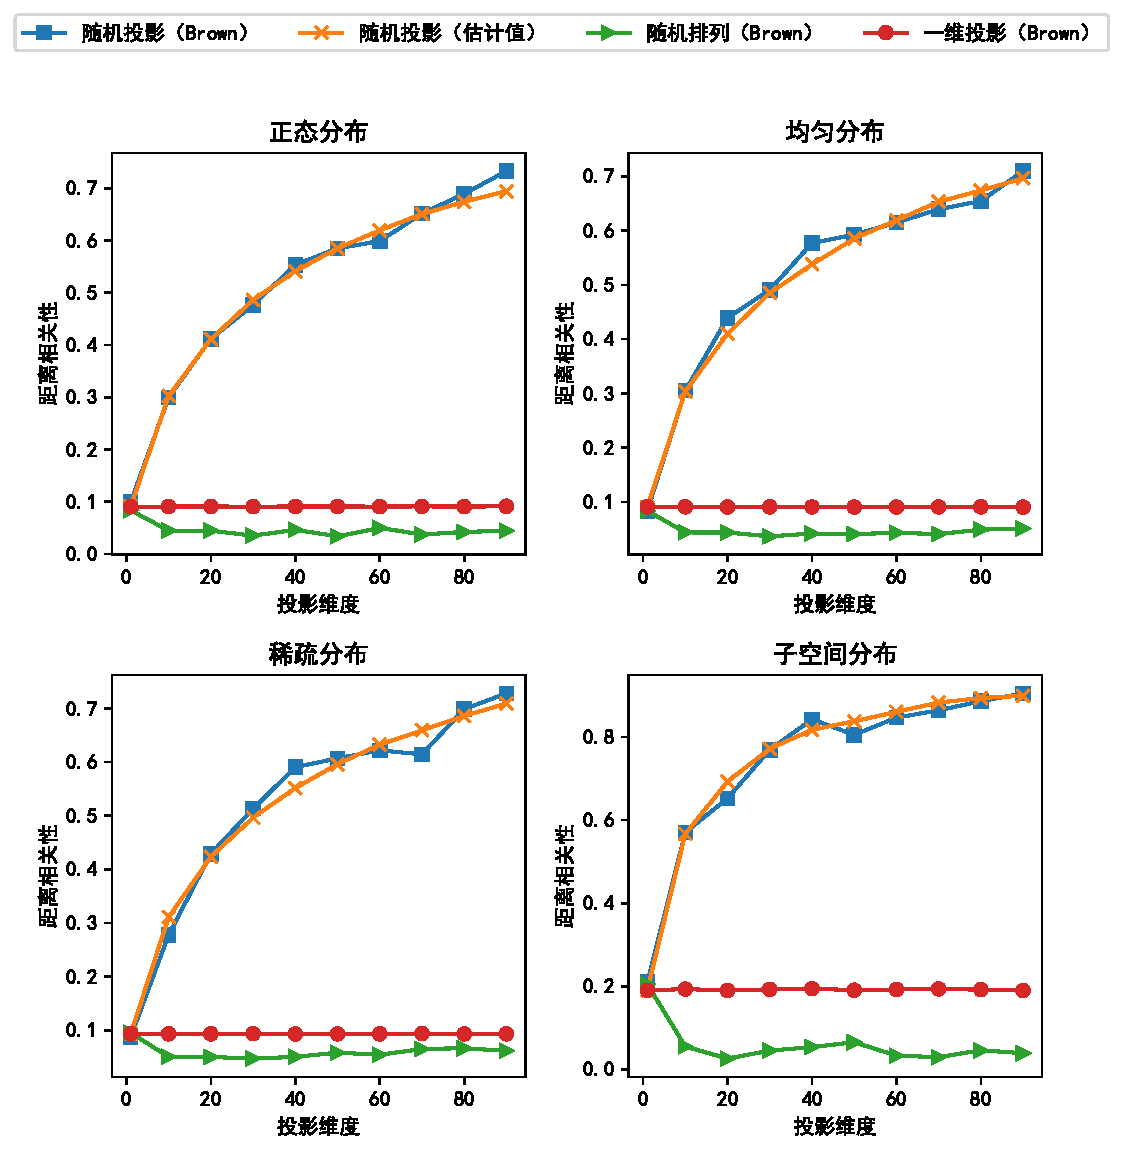
\includegraphics[width=\linewidth]{Z_Resources/ss-perm_dcor-estimation}
    \caption{各种数据分布下随机投影和随机排列的距离相关性}
    \label{fig:ss-perm:dcor-estimation}
\end{figure}


对于每个分布,我们采样1万个点(记作$X$),然后使用高斯分布的矩阵投影得到$Y = WX$,最后对投影后的向量进行随机排列得到$\pi[Y]$。
%
我们采用文献~\cite{szekely2009brownian_dcor}中的基于布朗运动(Brownian Motion)的方法对距离相关性进行数值计算(标记为“Brown”),同时也使用\autoref{eq:ss-perm:linear-dcor-estimation}对随机投影的距离相关性进行估算(标记为“估计值”),并一同呈现在\autoref{fig:ss-perm:dcor-estimation}中。
%


上述数值模拟表明,随机投影后的数据与原始数据具有较大的距离相关性,且投影后的维度越高,距离相关性越大。
%
而本文在投影后的数据上进一步采用随机排列,极大减少了距离相关性。
且无论投影维度变化,其距离相关性一直小于一维投影的距离相关性,验证了本节的理论分析结论。
\section{实验分析}
为了验证本章所提出的隐私保护神经网络框架的实用性,本节对本章的算法进行了实现。
%
我们基于Python的Numpy计算库~\cite{stefan_2011_numpy}实现了秘密分享的计算,其中秘密分享的整数环被选为$\mathbb Z_{2^{64}}$,因为64位整数能被计算机原生支持,可以方便地使用各种编程语言操作。
%
我们选择放缩系数为$2^{23}$,也就是对于任何实数(浮点数$x$),其整数表示为$x \cdot 2^{23}$。
此时定点数计算的精度达到$2^{-23}$,与32位浮点数的精确位一致~\cite{ieee_754_float},因此在该精度下神经网络的计算几乎不会有精度损失。
%
对于秘密分享中的通信交互,我们采用Python原生的套接字(Socket)接口进行编程,通过在节点之间建立持久化TCP连接的方式来交互数据,仅需初始化时的三次握手建立连接,防止其他上层协议带来的通信延迟。
同时我们采用流的方式进行数据读写,使用Pickle对变量进行打包。
%

\subsection{实验设置}
本节的实验在一台装备了16核Intel CPU,64GB内存的服务器上进行。
我们通过Linux自带的tc(Traffic Control)内核命令在本地网络(Localhost)上模拟了广域网(WAN, Wide Area Network)的带宽和延迟。
%
我们将WAN的带宽设置为80Mbps,将往返时间(Round Trip Time)设置为40ms。
%
这样的设置符合普通的家用宽带标准。
%
在实验开始之前,我们将训练数据以及初始化的神经网络权重秘密分享在$P_0$和$P_1$上。
%
我们对比了两个较新的密码学隐私保护神经网络方案,分别是SecureNN~\cite{wagh2019securenn}和ABY3~\cite{mohassel2018aby3}。
%
由于上述框架原始论文的开源代码未提供或无法运行,我们使用LatticeX-Rosetta库~\cite{latticex_rosetta}的SecureNN框架,以及TF-Encrypted库~\cite{tf_encrypted}的ABY3框架。
%
我们令所有的实验至少重复运行了10次,并把实验结果取平均值。


\begin{table}[h!]
\caption{逻辑回归的运行时间和通信量}
\label{tab:ss-perm:logistic}
\renewcommand{\arraystretch}{0.8}
\begin{tabular}{@{}cccrrrrrr@{}}
    \toprule
    \multicolumn{1}{l}{}     & \multicolumn{1}{l}{}    &    & \multicolumn{3}{c}{运行时间(秒)}       & \multicolumn{3}{c}{通信量(Mb)}       \\ 
    \cmidrule(lr){4-6}\cmidrule(lr){7-9}
    \multicolumn{1}{l}{输入维度} & \multicolumn{1}{l}{批大小} &    & 本方法            & SecureNN & ABY3  & 本方法            & SecureNN & ABY3  \\ 
    \cmidrule(lr){1-3}\cmidrule(lr){4-6}\cmidrule(lr){7-9}
    \multirow{4}{*}{100}     & \multirow{2}{*}{64}     & 推断 & \textbf{0.099} & 0.219    & 0.500 & \textbf{0.103} & 0.226    & 0.372 \\ \cmidrule(l){3-3}\cmidrule(lr){4-6}\cmidrule(lr){7-9}
        &                      & 训练 & \textbf{0.279} & 0.348 & 0.534 & \textbf{0.209} & 0.391 & 0.385          \\ \cmidrule(l){2-3}\cmidrule(lr){4-6}\cmidrule(lr){7-9}
        & \multirow{2}{*}{128} & 推断 & \textbf{0.108} & 0.228 & 0.500 & \textbf{0.202} & 0.448 & 0.624          \\ \cmidrule(l){3-3}\cmidrule(lr){4-6}\cmidrule(lr){7-9}
        &                      & 训练 & \textbf{0.281} & 0.367 & 0.539 & \textbf{0.413} & 0.775 & 0.639          \\ \midrule
    \multirow{4}{*}{1000}    & \multirow{2}{*}{64}     & 推断 & \textbf{0.132} & 0.358    & 0.511 & \textbf{0.996} & 1.072    & 1.369 \\ \cmidrule(l){3-3}\cmidrule(lr){4-6}\cmidrule(lr){7-9}
        &                      & 训练 & \textbf{0.294} & 0.698 & 0.831 & 1.988          & 2.581 & \textbf{1.678} \\ \cmidrule(l){2-3}\cmidrule(lr){4-6}\cmidrule(lr){7-9}
        & \multirow{2}{*}{128} & 推断 & \textbf{0.114} & 0.558 & 0.513 & 1.975          & 2.134 & \textbf{1.884} \\ \cmidrule(l){3-3}\cmidrule(lr){4-6}\cmidrule(lr){7-9}
        &                      & 训练 & \textbf{0.334} & 1.202 & 0.837 & 3.949          & 5.121 & \textbf{3.225} \\ \bottomrule
\end{tabular}
\end{table}

\begin{table}[h!]
\caption{神经网络的运行时间和通信量}
\label{tab:ss-perm:dnn}
\renewcommand{\arraystretch}{0.8}
\centering
\begin{tabular}{@{}cccrrrrrr@{}}
    \toprule
    \multicolumn{1}{l}{}  & \multicolumn{1}{l}{} &    & \multicolumn{2}{l}{运行时间(秒)} &      & \multicolumn{2}{l}{通信量(Mb)} &       \\ \cmidrule(lr){4-6}\cmidrule(lr){7-9}
    \multicolumn{1}{l}{模型} & \multicolumn{1}{l}{批大小} &    & 本方法           & SecureNN & \phantom{12}ABY3 & 本方法            & SecureNN & \phantom{12}ABY3           \\ \cmidrule(lr){1-3}\cmidrule(lr){4-6}\cmidrule(lr){7-9}
    \multirow{4}{*}{DNN1} & \multirow{2}{*}{64}  & 推断 & \textbf{0.19}     & 0.68    & 0.75 & \textbf{0.39}     & 1.98    & 1.90  \\ \cmidrule(l){3-3}\cmidrule(lr){4-6}\cmidrule(lr){7-9}
                            &                         & 训练 & \textbf{0.54} & 1.29     & 0.88 & \textbf{0.78}  & 4.05     & 2.21  \\ \cmidrule(l){2-3}\cmidrule(lr){4-6}\cmidrule(lr){7-9}
                            & \multirow{2}{*}{128}    & 推断 & \textbf{0.20} & 1.10     & 0.92 & \textbf{0.70}  & 3.89     & 3.63  \\ \cmidrule(l){3-3}\cmidrule(lr){4-6}\cmidrule(lr){7-9}
                            &                         & 训练 & \textbf{0.59} & 2.08     & 1.78 & \textbf{1.38}  & 7.90     & 4.10  \\ \midrule
    \multirow{4}{*}{DNN2} & \multirow{2}{*}{64}  & 推断 & \textbf{1.05}     & 5.67    & 1.86 & \textbf{10.69}    & 25.18   & 17.16 \\ \cmidrule(l){3-3}\cmidrule(lr){4-6}\cmidrule(lr){7-9}
                            &                         & 训练 & \textbf{1.86} & 12.11    & 3.24 & \textbf{17.97} & 55.98    & 35.20 \\ \cmidrule(l){2-3}\cmidrule(lr){4-6}\cmidrule(lr){7-9}
                            & \multirow{2}{*}{128}    & 推断 & \textbf{1.26} & 9.88     & 3.65 & \textbf{12.54} & 43.08    & 36.09 \\ \cmidrule(l){3-3}\cmidrule(lr){4-6}\cmidrule(lr){7-9}
                            &                         & 训练 & \textbf{2.58} & 20.00    & 5.14 & \textbf{24.84} & 93.19    & 47.71 \\ \bottomrule
\end{tabular}
\end{table}


\subsection{基准测试}
我们在逻辑回归模型以及全连接神经网络上对本方法和SecureNN~\cite{wagh2019securenn}、ABY3~\cite{mohassel2018aby3}框架进行了效率的评估,包含了运行时间、网络通信量的测量。

\textbf{逻辑回归}:
对于逻辑回归模型,我们把输入维度设置为100或1000,并把样本批次大小(Batch Size)设置为64或128。
实验结果汇报在\ref{tab:ss-perm:logistic}中。
可以看出,本章提出的方法相比于对比方法,训练或推断同时减少了2 -- 4倍,并且在大多数情况下也取得了更低的通信消耗。
%



\textbf{神经网络}:
我们测试了两种全连接神经网络模型,其输入维度分别为100和1000,云层大小分别为50和500。
样本批次大小也同样设置为64和128。
实验结果汇报在\ref{tab:ss-perm:dnn}中。
%
实验结果表明,相比于逻辑回归模型,本方法在神经网络上具有更高的优越性。
本方法相比于对比方法,在训练速度上有1.5 -- 5.5倍提升,同时减少了40\% -- 80\%的通信量。
这是因为神经网络的计算中有更多的非线性激活函数计算,使得本方法更多地发挥了在激活函数上的优势。
%



%
\begin{figure}[h!]
    \centering
    \begin{subfigure}[b]{0.48\linewidth}
    \centering
    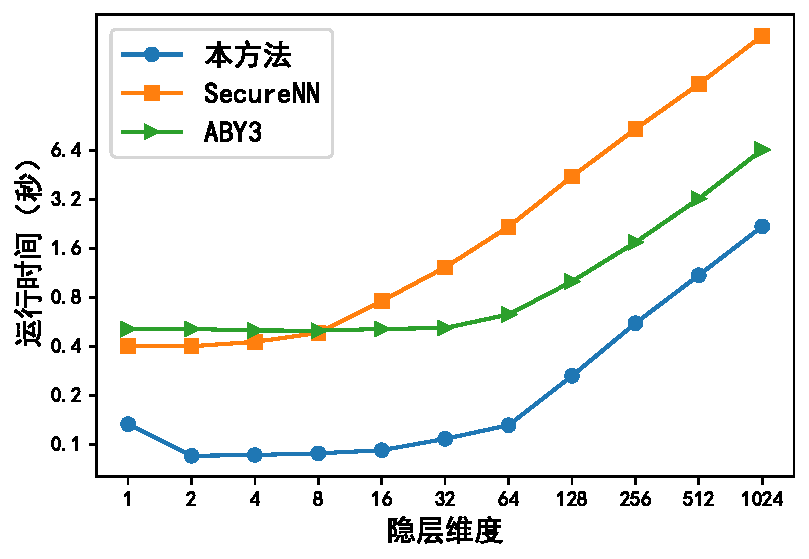
\includegraphics[width=\linewidth]{Z_Resources/ss-perm_one-layer-time.pdf}
    \caption{运行时间}
    \end{subfigure}
    %
    \begin{subfigure}[b]{0.48\linewidth}
    \centering
    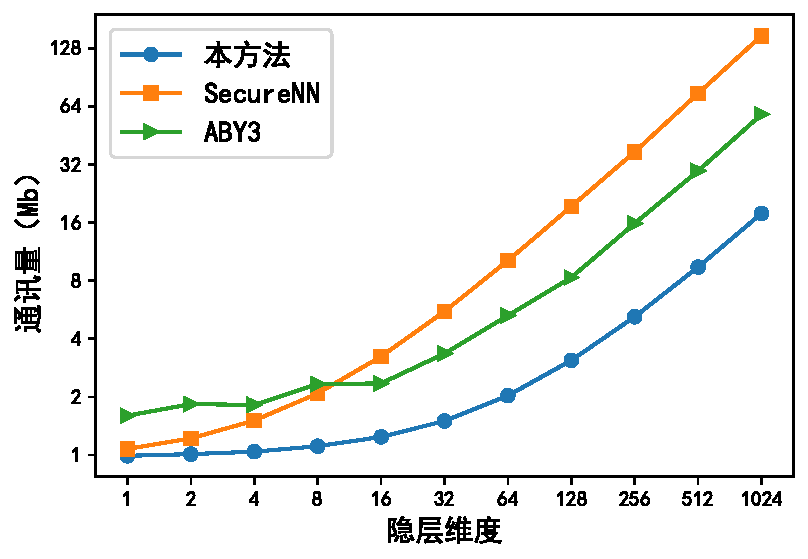
\includegraphics[width=\linewidth]{Z_Resources/ss-perm_one-layer-comm.pdf}
    \caption{总计通信量}
    \end{subfigure}
    
    \begin{subfigure}[b]{0.48\linewidth}
    \centering
    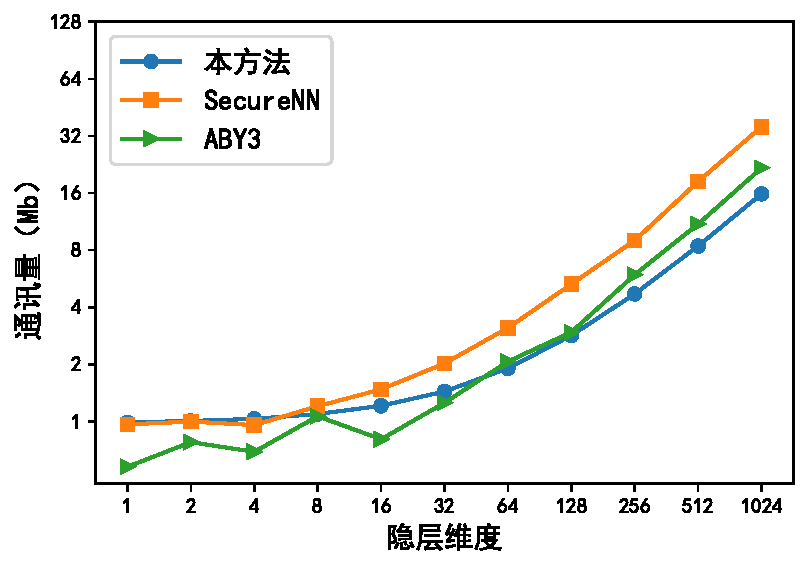
\includegraphics[width=\linewidth]{Z_Resources/ss-perm_one-layer-c01.pdf}
    \caption{$P_0$和$P_1$之间的通信量}
    \end{subfigure}
    %
    \begin{subfigure}[b]{0.48\linewidth}
    \centering
    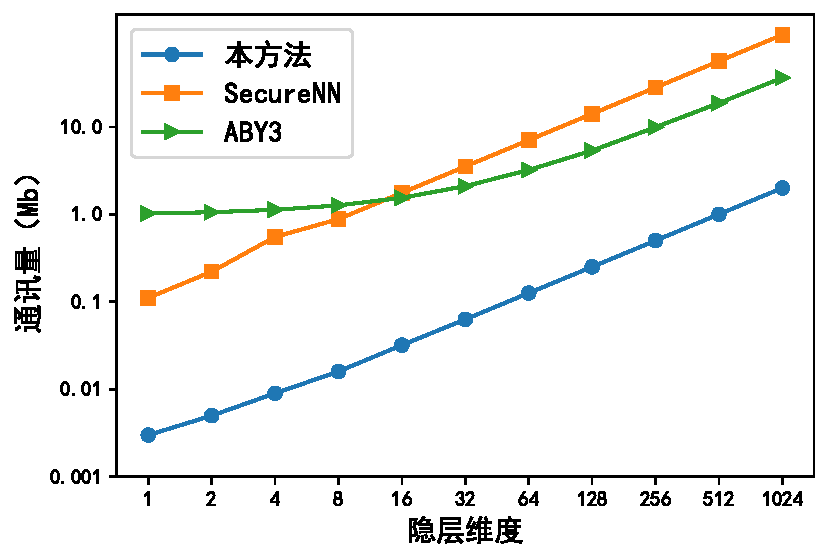
\includegraphics[width=\linewidth]{Z_Resources/ss-perm_one-layer-c2.pdf}
    \caption{$P_2$的通信量}
    \end{subfigure}
\caption{不同隐层维度时的运行时间和通信量}
\label{fig:ss-perm:layer-dim}
\end{figure}

\subsection{隐层维度对开销的影响}
为了测试本方法在不同大小的隐层上的效果,本节对本方法和对比方法在不同大小的神经网络隐层的运行时间以及通信量进行了测试,其中隐层的输入维度固定为1000。
%
本实验不仅测试了总计通信量,也测试了$P_0$和$P_1$之间的通信量和$P_2$相关的通信量。
%
实验结果呈现在\ref{fig:ss-perm:layer-dim}中。
%
可以看出,随着隐层维度逐步增加,本方法的优势逐渐扩大。
当隐层维度达到64左右时,本方法的所有通信量指标都是最低的。
%
本方法尤其减少了辅助第三方($P_2$)的通信量,相比于其他方法的通信量减少了大概1个数量级。
由于三种方法均采用秘密分享进行线性运算,因此$P_0$和$P_1$之间的通信量差距较小。

\subsection{真实数据集实验}
为了测试本章提出的方法在实际场景下的效果,本节对本章方法在真实数据下进行了实验,并且将其和明文训练进行对比,考察了训练准确率以及隐层经过随机排列后的隐私泄露程度。

\subsubsection{准确率}
为了验证本方法的训练准确率,我们在Gisette数据集~\cite{2008_gisette}和MNIST数据集~\cite{mnist}上分别使用本方法进行了训练,同时与明文对比,并绘制出验证集准确率随着训练轮数变化的曲线图在\autoref{fig:ss-perm:train}a-c中。

%
Gisette数据集~\cite{2008_gisette}是一个二分类数据集,包含了6000个训练样本和1000个测试样本,特征维度为5000。
我们用逻辑回归模型对其进行了训练。
%
MNIST数据集~\cite{mnist}是一个10分类的手写数字分类数据集,包含了60000个训练样本和10000个验证样本。
我们用两个全连接神经网络(DNN1、DNN2)对其进行训练,其结构分别为784-128-10和784-128-32-10,DNN2的第一个隐层激活函数为ReLU,其余隐层采用Sigmoid作为隐层激活函数。

实验结果表明,采用本方法的隐私保护逻辑回归和神经网络的训练曲线与明文神经网络的训练曲线几乎重合,说明本方法带来的训练精度损失可以忽略不计。

\begin{figure}[h!]
    \centering
    \begin{subfigure}[b]{0.47\linewidth}
    \centering
    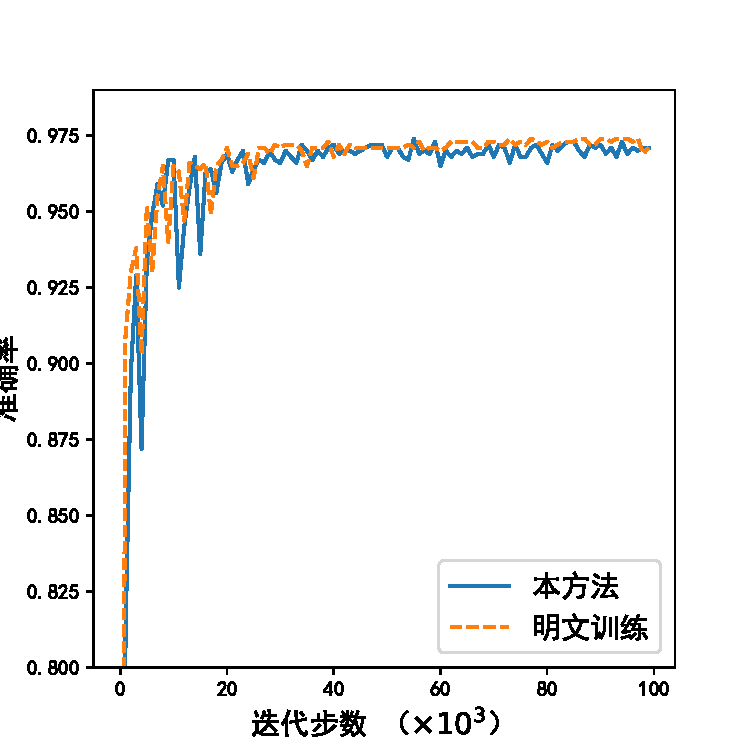
\includegraphics[width=\linewidth]{Z_Resources/ss-perm_lr.pdf}
    \caption{Gisette数据集逻辑回归训练曲线}
    \end{subfigure}
    %
    \begin{subfigure}[b]{0.47\linewidth}
    \centering
    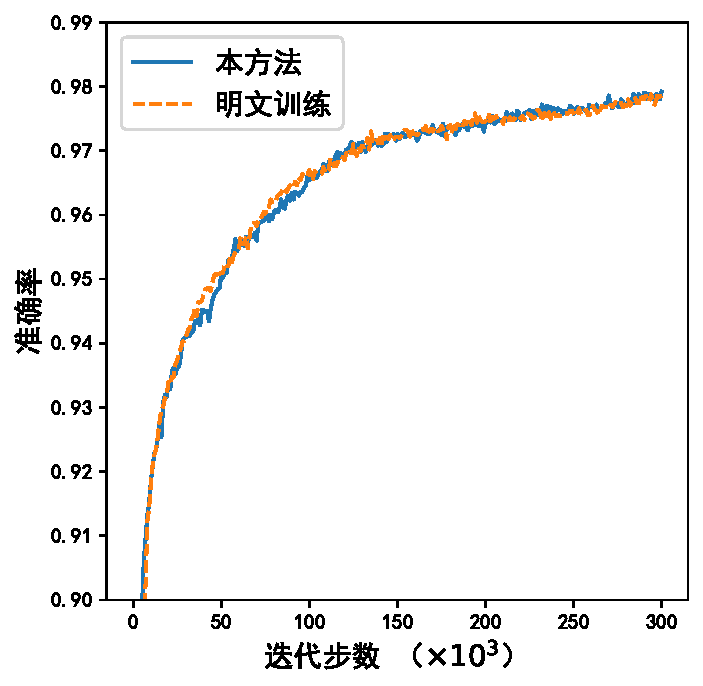
\includegraphics[width=\linewidth]{Z_Resources/ss-perm_dnn1.pdf}
    \caption{MNIST数据集DNN1训练曲线}
    \end{subfigure}
    
    \begin{subfigure}[b]{0.47\linewidth}
    \centering
    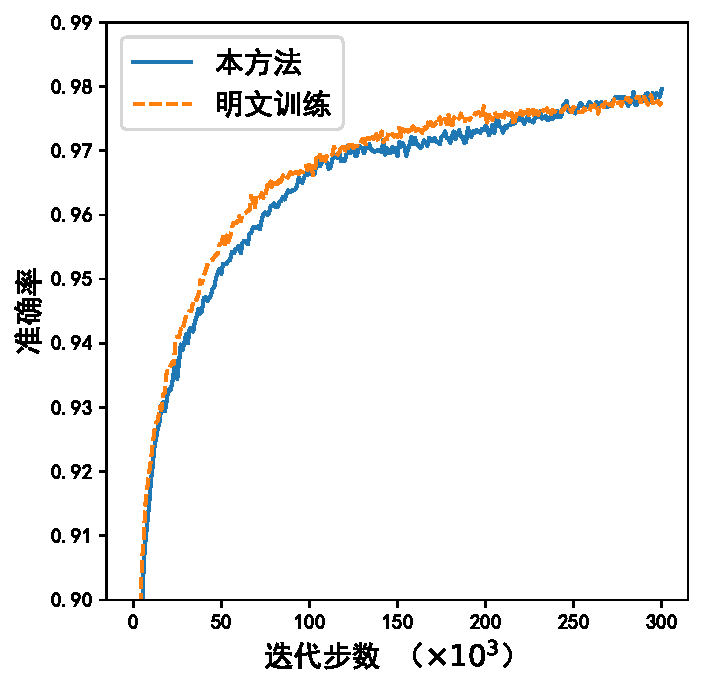
\includegraphics[width=\linewidth]{Z_Resources/ss-perm_dnn2.pdf}
    \caption{MNIST数据集DNN2训练曲线}
    \end{subfigure}
    %
    \begin{subfigure}[b]{0.47\linewidth}
    \centering
    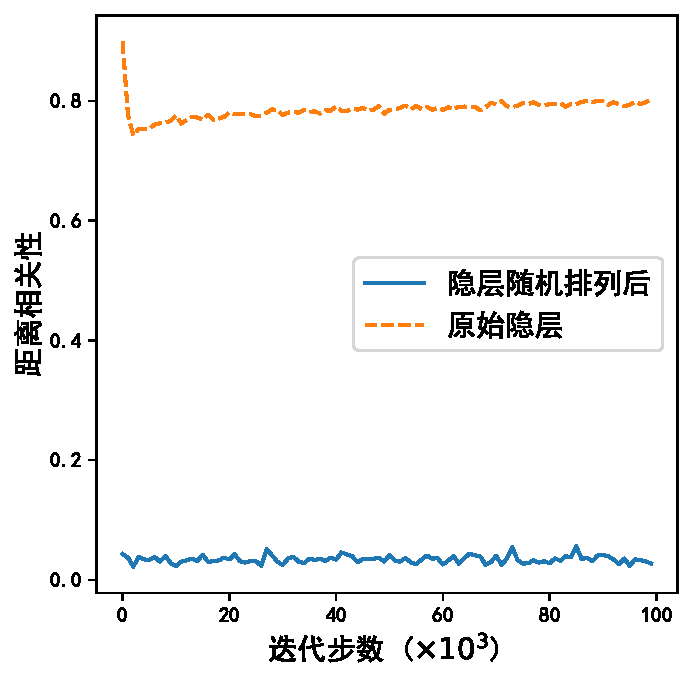
\includegraphics[width=\linewidth]{Z_Resources/ss-perm_dnn1-dcor.pdf}
    \caption{MNIST数据集DNN1隐层距离相关性}
    \end{subfigure}
\caption{在Gisette和MNIST数据集上的训练结果}
\label{fig:ss-perm:train}
\end{figure}

\subsubsection{隐层隐私泄漏情况}
我们在\autoref{fig:ss-perm:train}c中展现了DNN1隐层与输入的距离相关性,以及本方法暴露的数据(随机排列后的隐层)与输入的距离相关性。
%
可以看出,隐层与输入的距离相关性较高,在整个训练过程中维持在0.8左右的水平。
而随机排列后的隐层数据,其距离相关性大幅度降低到0.1以下,表明随机排列后的数据几乎不会带来隐私泄露。
%


另外,我们也测试了MNIST数据集中,基于隐层表征查找相似样本的结果。
%
为了考察在特殊情况下的安全性,提高隐私保护的难度,我们令一批样本全部为同一类别,因此随机排列并不能引入其他类别样本的信息。
%
实验结果呈现在\autoref{fig:ss-perm:permutation-attack}中。
%
其中最左边的列表示原始样本,蓝色方框表示框内的样本被合并为单个向量来进行随机排列。


\begin{figure}[h!]
    \centering
    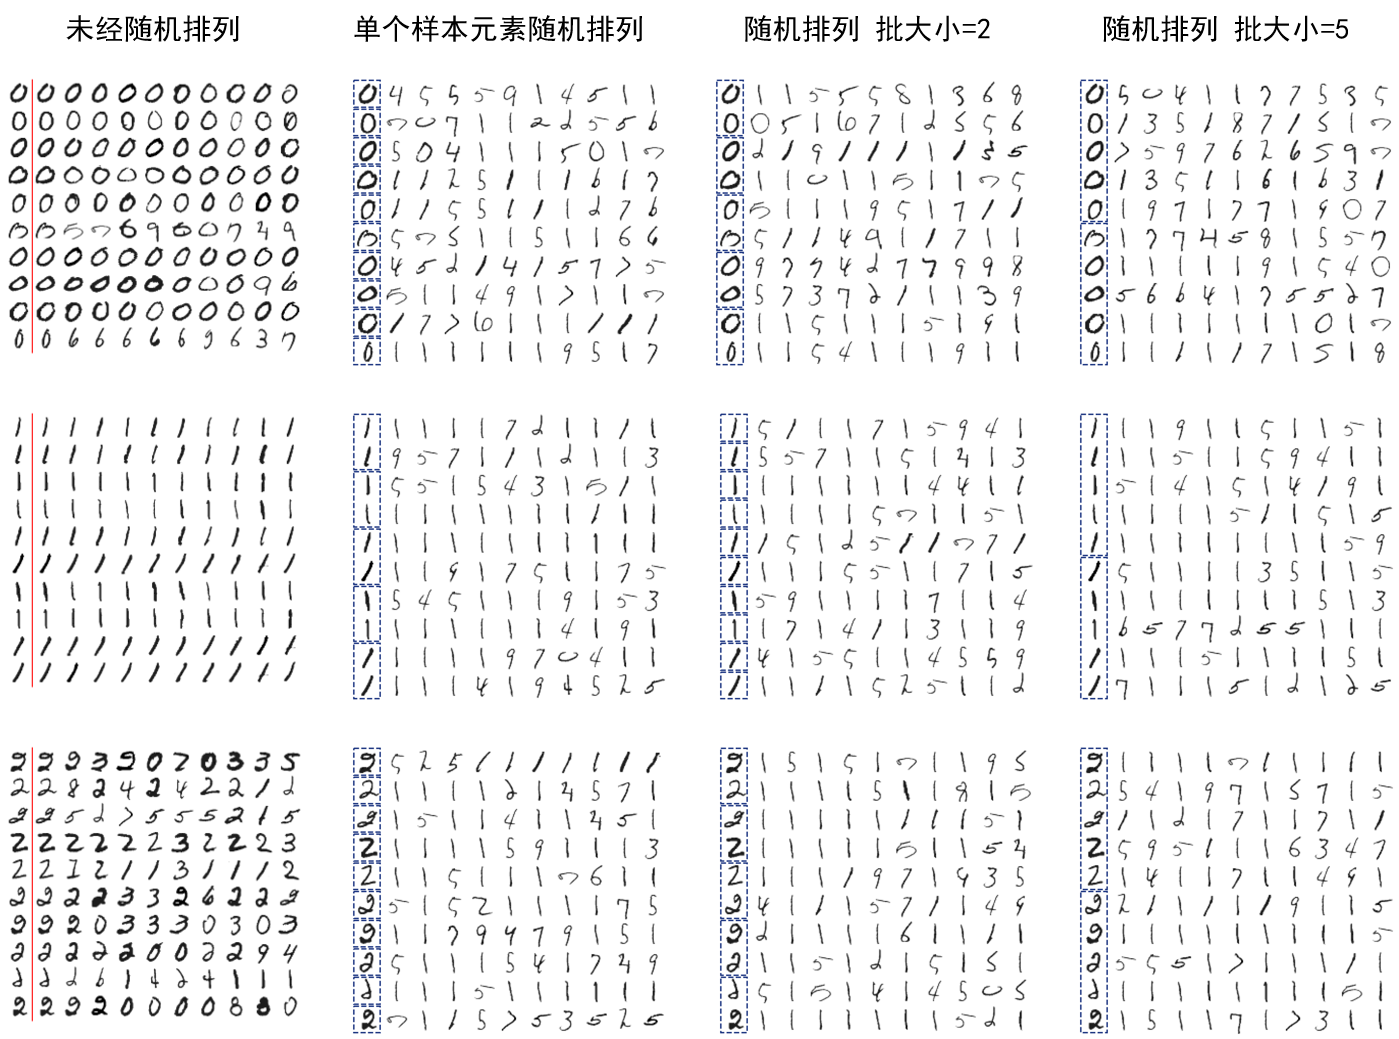
\includegraphics[width=\linewidth]{Z_Resources/ss-perm_permutation-attack.png}
    \caption{隐层表征随机排列前后的相似样本示意图}
    \label{fig:ss-perm:permutation-attack}
\end{figure}

实验结果表明,如果没有进行随机排列,也就是直接暴露隐层表征时,攻击者很容易根据隐层表征找到相似的样本。
%
而采用了随机排列之后,则攻击者找到的相似样本和原始样本无关。
%
无论原始样本属于哪个类别,找到的相似样本都是一些笔画较细的“1”等图像。
%
这是因为两个隐层表征$\bvec x, \bvec y \in \mathbb R^d$之间的距离可以用表示为
$\mathbb E_i [(x_i - y_i)^2] = \mathbb E_i [x_i^2 + y_i^2 - 2x_i y_i]$。
%
当$\bvec x, \bvec y$归一化后且$x_i, y_i$之间没有相关性时,则上式可以进一步表示为
$\mathbb E_i [x_i^2] + \mathbb E_i [y_i^2]$。
%
注意到$x_i, y_i \ge 0$。
%
因此,若$\mathbb E_i [y_i^2]$越小,就会导致$\mathbb E_i [(x_i - y_i)^2]$越小。
%
而较小的$\mathbb E_i[y_i^2]$对应是分布更加集中的$\bvec y$,其输入大概率是黑色像素较少的图片,因为MNIST数据集的图像以白色部分为主。
%

\section{本章小结}
    \chapter{基于随机排列的高效大语言模型推理框架}
\section{研究背景}
2023年ChatGPT的出现,标志着人工智能的发展到达了一个新的阶段~\cite{chatgpt}。
%
ChatGPT以及类似的大语言模型(Large Language Models),通过利用大量的语料进行自回归训练以及人类反馈强化学习,从而实现了与人类进行自然对话的能力,并且在大量任务上都达到了最先进水平~\cite{}。
%
通过提示词,大模型可以完成多种多样的任务,其效果往往超过此前研究者针对该任务精心设计的模型~\cite{}。
%
因此,当前大语言模型成为了学术界和业界的焦点,基于大语言模型的应用也层出不穷,包括了各种领域的问题回答(Question Answering)、阅读理解(Reading Comprehension)、文本生成(Text Generation)、检索增强(Retrieval Augmented Generation)等~\cite{}。


在大模型被广泛应用的同时,其隐私问题也愈加突出。
%
大模型的训练成本极大,据估计,一个GPT-3模型训练的计算成本已经高达数百万美金。
%
因此,大模型的模型参数是公司的重要资产,不能直接以开源的方式提供给用户。
%
在这种情况下,用户必须调用模型拥有方(如OpenAI公司)提供的接口(API)来使用大模型。
%
用户将自身的输入文本发送给模型拥有方的服务器,服务器上执行明文的大模型推断,然后将结果返还给用户。
%
在这个过程中,用户输入文本的隐私就被完全暴露给了模型拥有方。
%
这带来了极大的隐私泄漏风险。
%
例如,三星公司的员工使用ChatGPT分析了公司内部的机密数据,使得三星公司开始禁止员工使用类似的大模型工具~\cite{}。
%
因此,上述的隐私泄露风险给大语言模型的应用产生了一定程度的阻碍。


为了解决大模型的隐私问题,在应用大模型时同时保护用户输入和模型参数的隐私,一些研究基于密码学方法提出了初步的解决方案。
%
这些方法一般采用已有的秘密分享或同态加密方案来实现大模型中的线性运算,然后采用高阶多项式拟合的方式来实现大模型中的非线性运算,如GeLU、Softmax等。
%
但是由于采用密码学的隐私保护机器学习框架自身会带来巨大的额外开销,加之大模型的参数规模和运算量十分庞大,上述方法即使在理想的计算资源与网络环境下,也至少需要消耗几分钟时间、数十GB流量才能产生一个输出单词。
%
因此,基于密码学方法的大模型隐私推断框架的实用性依然欠缺,并且可以预见到使用已有的密码学底层算法很难实现具备实用性的大模型隐私推断。
%
如何在保护输入的模型隐私的基础上,实现高效安全的实现大模型推断,依然是一个亟待解决的问题。

\section{初步研究}
本节我们对大语言模型的模型结构进行初步的介绍和分析,并从理论和实验两方面分析使用拆分学习进行大模型隐私推断时的严重隐私泄漏问题。

\subsection{大模型结构}
当前的大语言模型都是基于Transformer架构~\cite{vaswani_2017_attention}实现的,其模型可以分为3层,分别是:
\begin{enumerate}
    \item 输入词向量(Word Embedding):即一个嵌入向量矩阵$E \in \mathbb R^{n\times d}$,其中$n$表示词汇表大小,$d$表示词向量的维度,一般为4096。
    %
    当输入$n$个单词(Token)后,其输出为$n \times d$大小的矩阵。
    %
    \item Transformer层:包含了多层Transformer结构,对隐层表征进行多次变换,其输入和输出的矩阵大小均为$n \times d$(此处忽略批样本情况,进考虑三个样本)。
    \item 输出词向量:与输入词向量相同,包含了一个矩阵$E' \in \mathbb R^{n\times d}$,且一般来说$E' = E$。
    当获得Transformer层的输出后,对输出的最后一行计算分数$\bvec  s = E'\bvec h$,表示输出单词的概率分布。
\end{enumerate}

其中Transformer层的关键模块是多头自注意力机制(Multi-Head Self-Attention,简称MHA)。
%
该模块会融合文本中不同位置单词(上下文)的信息产生输出,而其他模块仅仅对当前位置的表征进行变换。
%
具体而言,对于隐层表征$H \in \mathbb R^{n\times d}$,多头自注意力机制的运算包含如下步骤:
\begin{enumerate}
    \item 产生查询(Query)、键(Key)、值(Value)对应的向量:对于任意一个位置的隐层表征$\bvec h \in H$,通过线性投影产生对应的$\bvec q = W_q \bvec h, \bvec k = W_k \bvec h, \bvec v = W_v \bvec h \in \mathbb R^d$。
    %
    \item 将所有的查询、键、值向量分割为维度为$d'$的子向量(注意力头),总共$d/d'$个,并对其进行位置嵌入(Positional Embedding)变换,一般而言是对向量逐元素地加或乘一个固定并和当前单词相关的向量。
    %
    \item (对于每个注意力头)对于第$i$个查询$\bvec q_i'$,将其与当前存在的所有的键作内积得到分数$s'_{i, j} = \bvec q_i' \cdot \bvec k_j, j = 1\cdots n$。
    对这些分数进行Softmax归一化后再计算加权的值向量和 $\bvec h'_i = \dfrac{\exp {s'_{i, j}}}{\sum_{k = 1}^n \exp {s'_{i, k}}} \cdot \bvec v_j \in \mathbb R^{d'}$,这是当前的注意力头的输出。
    %
    \item 将各个注意力头的输出拼接起来,得到多头注意力的输出$\bvec h_i = \mathsf{concat}(\cdots, \bvec h'_i, \cdots)$。
\end{enumerate}

从上述分析中可以看出,注意力机制将不同位置(也就是不同输入单词)对应的表征进行了相互融合,从而捕捉文本中上下文的关系。
%
大语言模型在生成文本时,需要采用迭代生成的方式,即将前一轮的输出单词拼接到当前的输入语句中,然后再次输入模型预测下一个单词。
%
由于我们仅仅需要最后一个单词对应的表征,我们可以把之前MHA中计算出来的键向量和值向量缓存下来,从而只需要把最后一个单词输入模型中即可计算,从而避免重复计算。
%
这种技术被称为键值缓存(KV Cache)~\cite{pope_2023_efficiently_kv_cache}。
%
Transformer的其他模块包括全连接层(Fully-Connect Layer)、层归一化(Layer Normalization)模块,以及残差连接,是普通神经网络中的常用模块,在此不再赘述。
%
\autoref{fig:perm-llm_llm-arch}展现了一个典型的大语言模型的网络结构。

\begin{figure}[htbp]
    \centering
    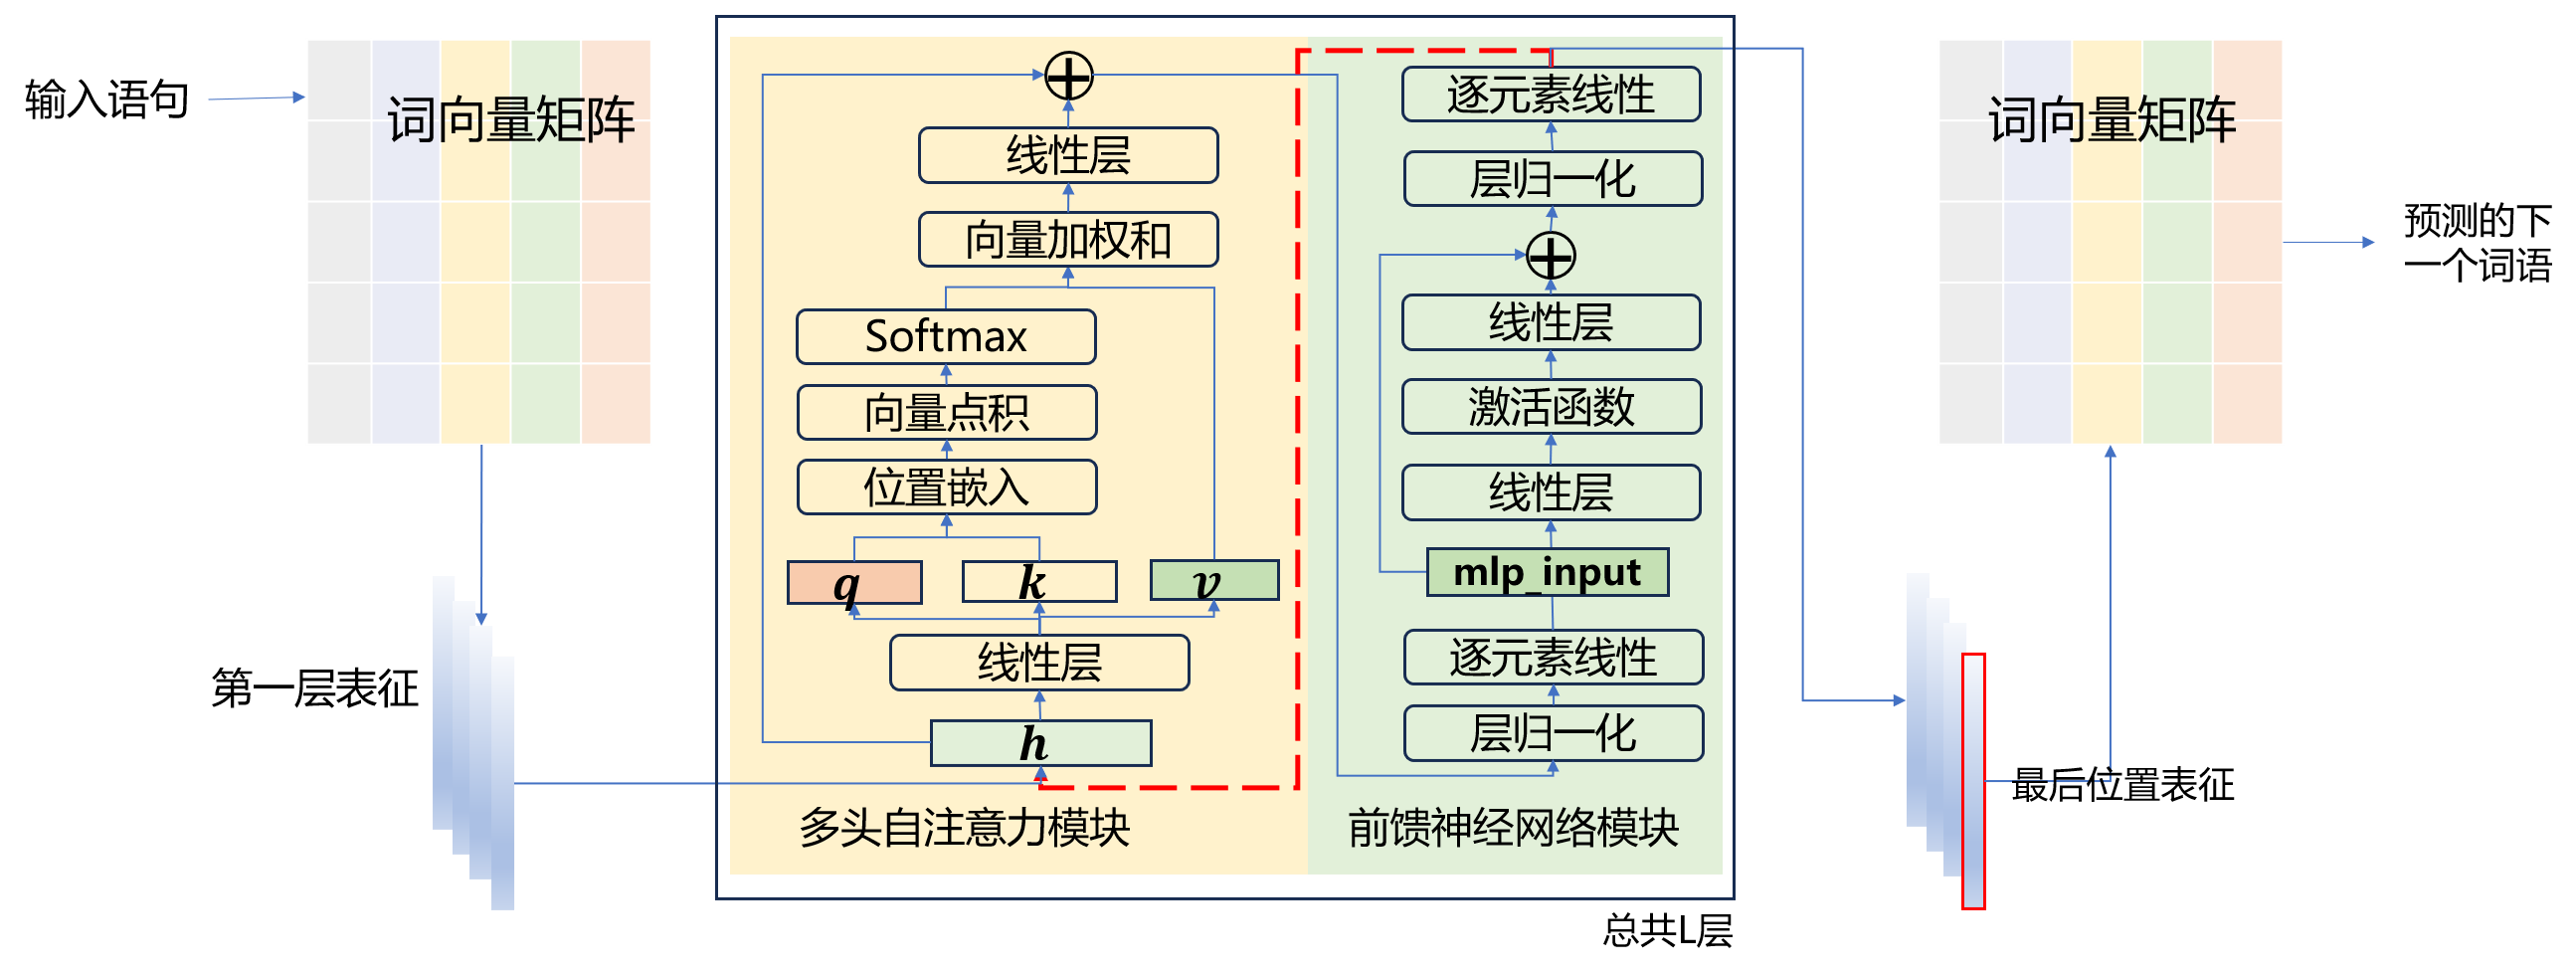
\includegraphics[width=\linewidth]{Z_Resources/perm-llm_llm-architecture.png}
    \caption{大语言模型结构示意图}
    \label{fig:perm-llm_llm-arch}
\end{figure}


\subsection{针对大模型拆分学习的攻击}
从上节的大模型结构描述中可以看出,大模型的隐层表征在每一层Transformer的变换中都保持着同样的大小,即$n \times d$($n$ 表示输入语句长度,$d$表示表征维度)。
%
因此从直观角度理解,大模型隐层表征包含了大量的输入信息。
且由于其隐层表征的尺寸随着层数增加保持不变,可以猜测即使是高层的隐层表征,依然包含着足够多的输入数据的信息。
%
已有研究提出可以通过训练逆向模型的方式从表征中恢复原始原本,无需知道模型的具体参数~\cite{morris2023embedding_almost}。
而本节则考虑攻击者已知模型参数的情况,更符合大模型的应用场景。


在拆分学习的大模型推断场景中,大模型被划分为一个底部模型$M_b$和一个顶部模型$M_h$。
%
我们假设模型拥有方最初拥有整个模型$(M_b, M_h)$,这也符合当前大模型训练是中心化的实际情况。
%
为了实现拆分学习的推断,模型拥有方将$M_b$发送给用户。
%
这种情况下,用户需要发送底部模型产生的表征$\bvec h = M_b(\bvec x)$给模型拥有方,其中$\bvec x$表示用户的输入文本对应的下标向量。

\subsubsection{表征逆向攻击}
当模型拥有方获取用户输入的表征后,就可以进行白盒攻击~\cite{hezecheng_2019_model_inversion_attack},通过如下的优化问题来猜测用户的输入:
\begin{equation}
    \label{eq:perm-llm_split-attack-0}
    \min \Vert M_b(\bvec x') - M_b(\bvec x)\Vert^2,
\end{equation}
其中$\bvec x'$是模型拥有方猜测的用户输入,$\bvec x$是用户的实际输入。
%
注意到直接对$\bvec x'$进行优化是较为困难的,因为其值域是离散的单词下标。
虽然可以转化成读热向量(One-Hot Vector),但是其依然具有离散的约束从而导致优化难以进行。
%
为此,模型拥有方可以首先优化初始表征$H'$,也就是词向量矩阵与(猜测的)用户输入对应的独热向量乘积:$H'_i = E\ \mathsf{onehot}(x'_i)$。
%
我们让$T_b$为底部模型除去词向量层(第一层)产生的模型,则我们可以把\autoref{eq:perm-llm_split-attack-0}改写为
\begin{equation}
    \label{eq:perm-llm_split-attack-1}
    \min \Vert T_b(H') - M_b(\bvec x)\Vert^2.
\end{equation}
由于此时优化变量$H'$属于连续变量,同时注意到$T_b$是模型拥有方已知的,因此我们可以直接用梯度下降等方法对\autoref{eq:perm-llm_split-attack-1}进行优化。
%
此时上述优化问题的未知数个数($H'$中的元素个数)与方程个数相等($M_b(\bvec x)$的元素个数),均为$nd$个元素,因为我们认为这个优化问题可能存在唯一的最优解,也就是$H' = H := (E\ \mathsf{onehot}(x_1), \cdots, E\ \mathsf{onehot}(x_n))$。
%
当得到猜测的表征$H'$之后,对于其中的第$i$行,使用余弦相似度计算出其最相似的词向量:
\begin{equation}
    \text{最相似单词下标} = \mathop{\text{argmax}}_i \dfrac{\bvec h'_i \cdot \bvec e_i}{\Vert \bvec h'_i \Vert\Vert \bvec e_i \Vert},
\end{equation}
其中$\bvec e_i$表示词向量矩阵的第$i$行。

综上所述,从大模型隐层表征恢复出用户输入文本的过程可以分为恢复第一层表征和从第一层表征恢复单词两步。
%
通过上述提出的两步方法,攻击者可以从隐层表征逆向推理出输入文本中每一个位置的单词,从而窃取用户的输入数据。
%

\subsubsection{可能的防御机制}
对数据加噪声是一种常用的隐私保护方法,并且在特定情况下可以达成差分隐私~\cite{dwork_2006_differential_privacy}。
%
因此,本节我们考虑在隐层表征中加入噪声进行防御的手段~\cite{morris2023embedding_almost}。
%
当用户算出底部模型产生的表征$H$后,对其进行扰动得到
\begin{equation}
    \tilde H_{ij} = H_{ij} + \lambda \cdot \epsilon, \quad \epsilon \sim \mathcal N(0, 1), 
\end{equation}
其中,$\lambda$表示噪声的大小。
%
越大的噪声一般可以实现越好的保护效果,但是也会产生更多的精度损失,损害模型性能。

\subsubsection{实验分析}
为了进一步测试上述攻击方案的可行性,我们在ChatGLM-6B模型~\cite{zeng_2022_glm130b}上进行了实验。
%
我们选用了Squad~\cite{2016_squad}和FindSum~\cite{2022_findsum}两个数据集进行实验,分别对应较短的文本和较长的文本。
%
对于每个实验,我们都对200个输入进行测试并且求其平均值。
%
攻击准确率的定义如下:
\begin{equation}
    \text{准确率} = \dfrac{1}{n} \sum_{i=1}^n \left( \dfrac{1}{l_i} \sum_{j=1}^{l_i} 1_{t'_{i,j} = t_{i,j}} \right),
\end{equation}
其中,$n = 200$表示总共的输入文本数,$l_i$表示第$i$个文本的长度,$t'_{i,j}$和$t_{i,j}$表示攻击得到的和实际的第$i$个文本的第$j$个单词。
%
由于ChatGLM-6B模型总共包含了28个Transformer层,我们设置拆分层分别为第10层和第20层。
%
我们使用梯度下降算法迭代优化\autoref{eq:perm-llm_split-attack-1}直到$H'$和$H$的余弦相似度达到0.98或迭代步数达到1000步为止。
%
我们使用半精度浮点数进行运算。

\begin{figure}[h!]
    \centering
    \begin{subfigure}{0.48\linewidth}
    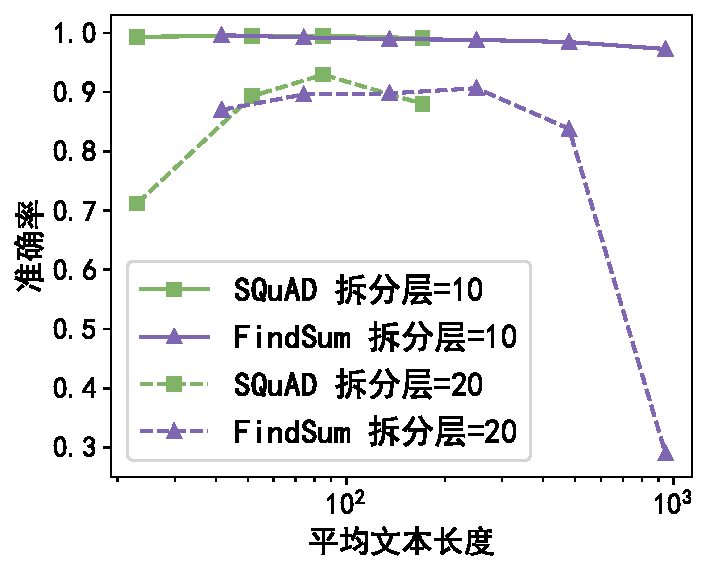
\includegraphics[width=\linewidth]{Z_Resources/perm-llm_seqlen-acc.pdf}
    \caption{攻击准确率}
    \end{subfigure}
    %
    \begin{subfigure}{0.48\linewidth}    
    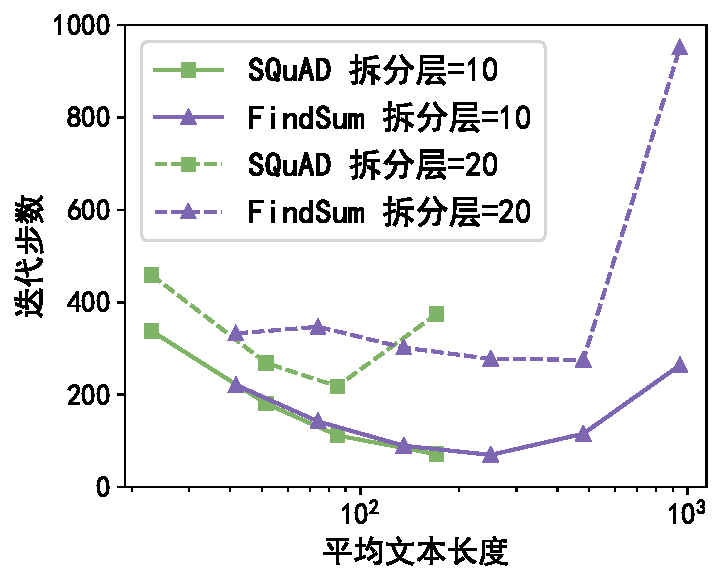
\includegraphics[width=\linewidth]{Z_Resources/perm-llm_seqlen-steps.pdf}
    \caption{攻击所需迭代步数}    
    \end{subfigure}
    \caption{攻击效果与文本长度的关系}
    \label{fig:perm-llm:attack-seqlen}
\end{figure}


\begin{figure}[h!]
    \centering
    \begin{subfigure}{0.48\linewidth}
    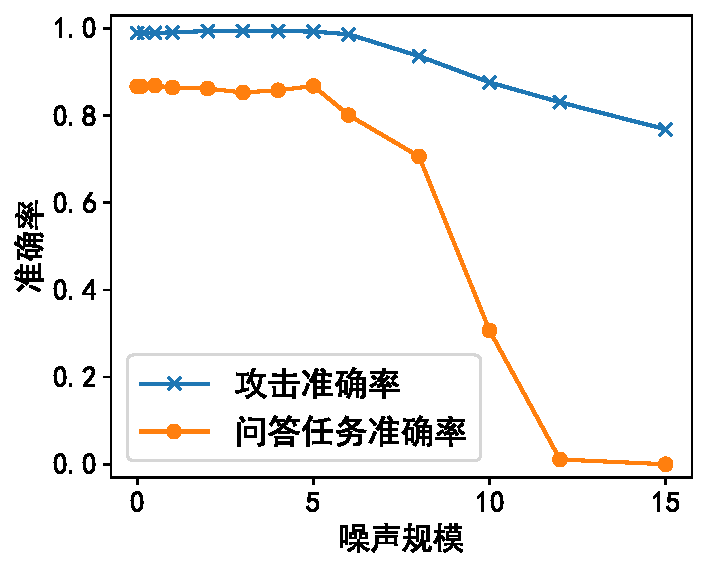
\includegraphics[width=\linewidth]{Z_Resources/perm-llm_squad-noise-layer10.pdf}
    \caption{拆分层=10}
    \end{subfigure}
    %
    \begin{subfigure}{0.48\linewidth}    
    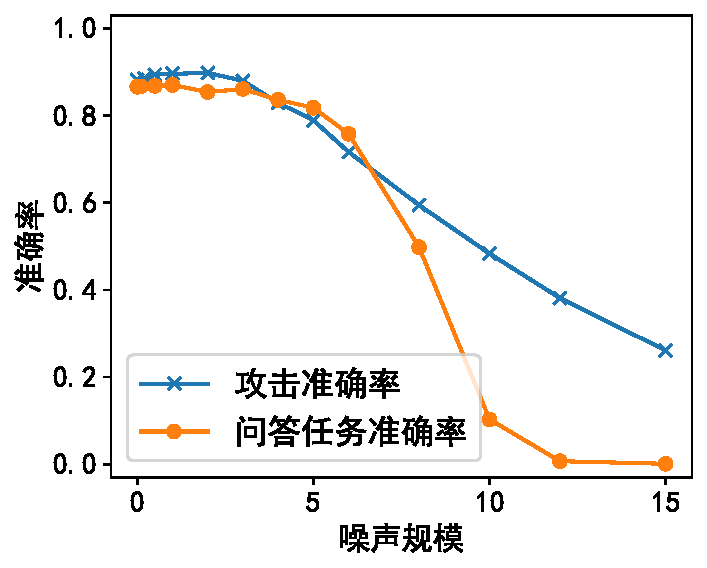
\includegraphics[width=\linewidth]{Z_Resources/perm-llm_squad-noise-layer20.pdf}
    \caption{拆分层=20}    
    \end{subfigure}
    \caption{攻击效果与噪声大小的关系}
    \label{fig:perm-llm:attack-noise}
\end{figure}

%
我们首先测试了对于不同输入语句长度的逆向攻击效果,测量了窃取用户输入文本的准确率以及迭代所用次,并呈现在\autoref{fig:perm-llm:attack-seqlen}中。
%
从图中可以看出,在拆分层为第10层时,无论文本长度多长,攻击都能达到接近100\%的准确率;而拆分层在20层时,攻击准确率略有下降,大概为90\%左右。
同时我们注意到,文本长度特别长(1000左右)或特别短(个位数)时,攻击效果也会下降。
%
特别是文本长度达到1000时,攻击效果下降明显,但是此时迭代步数也达到了我们预设的最高值,因此可能在更多的迭代步数下会达到更高的效果。
%
此外,提高浮点运算的精度(比如从16位半精度提升到32位单精度)也可能会提升攻击效果。


我们也在Squad数据集上测试了噪声规模$\lambda$的大小对攻击效果以及原始任务效果的影响。
其中原始任务的准确率指的是问答任务的准确率,按照大模型返回的字符串中是否包含参考答案的字符串来计算,若包含则为回答正确,反之则为回答错误。
%
我们将结果汇报在\autoref{fig:perm-llm:attack-noise}中。
%
可以看到,随着噪声规模的增加,攻击准确率呈现出下降趋势。
然而原始的问答任务准确率也同步开始下降,并且下降速度更快。
%
在拆分层为第10层时,当问答任务的准确率已经变成0之后,攻击准确率依然有80\%以上。
在拆分层为第20层时,两者的下降幅度更加接近,但是问答任务准确率依然在$\lambda \ge 5$后下降的更快并且更快归零。
%



上述的实验分析表明,攻击者可以通过大模型拆分层的表征,有效地以很高精度还原出用户的原始输入。
%
对拆分层表征添加噪声的防御手段并不能有效地避免此种攻击。
%
这说明拆分学习不适用于大模型隐私推断的场景。

\section{PermLLM框架}
经过前文的梳理和分析,我们可以看到拆分学习应用于大模型的隐私推断存在严重的隐私泄漏问题,与此同时,密码学方法则存在着严重的计算通讯开销问题。
%
我们注意到,密码学在进行大模型隐私推断时,其主要的开销也在于非线性激活函数GeLU上。
由于GeLU的非线性较强,各种密码学方案往往采用高阶多项式对其进行拟合,从而带来了严重的计算开销。
%
现有研究的分析表明,GeLU、层归一化等的通讯开销甚至可以达到线性计算(矩阵乘法等)的一百多倍。
%
因此,优化基于密码学的大模型隐私推断的关键在于优化非线性函数。
%
%

而上一章提出的基于秘密分享和随机排列的安全神经网络框架正是对神经网络的非线性激活函数进行优化,极大提高了神经网络隐私推断和训练的效率,同时尽可能地维持了安全性。
%
在此基础上,本章我们对此针对大模型进行进一步优化,提出融合密码学方法和随机排列的基础上,实现高效安全的大模型隐私推断框架PermLLM。
%
PermLLM框架面向的场景为两方推断的场景,且存在一个辅助第三方用于离线计算。
%
$P_0$为模型拥有方(如OpenAI),其拥有模型的所有参数信息。
%
$P_1$为用户,其目标是获取大模型的关于自身的文本输入的回复。
%
$P_2$为辅助第三方,其参与离线计算阶段,用于生成安全乘法和安全排列的预计算值。
%
我们采用了半可信的安全性设定,同\autoref{}一致。


我们将大语言模型的计算分为三个部分:线性部分、非线性部分和下标选择阶段。
其中线性阶段包含了线性层、注意力分数计算、层归一化后的逐元素线性映射等;
非线性阶段包含了GeLU激活函数、注意力分数的Softmax计算、层归一化的计算等;
而下标选择阶段则是根据预测的分数安全地产生预测词语的下标的阶段。
%
对于线性阶段,我们通过改进的秘密分享协议进行高效计算;
对于非线性阶段,我们采用基于安全随机排列协议的逐元素计算协议进行计算;
对于下标选择阶段,我们基于随机排列和同态加密设计了安全的下标选择协议,不仅支持常用的选取最大分数的词语,也支持按照概率采样等复杂的下标选择策略。
%


\subsection{隐私推断的三个阶段}
许多基于秘密分享技术的隐私保护机器学习框架会按照两个阶段运行,分别是离线(Offline)阶段和在线(Online)阶段。
%
考虑$P_0$和$P_1$要安全地计算$f(X)$的情况,其中$X$被秘密分享在两方之间,而$f$则是一个固定的函数。
%
在离线阶段,$X$还未出现,$P_0$和$P_1$并不需要知道$X$的具体值。
%
但是其可以对未来的$f(X)$进行一些准备工作,比如生成Beaver三元组来辅助安全乘法计算。
%
在在线阶段,$P_0$和$P_1$得到了$X$的具体值,再进行后续的工作。
%t
通过这种方法,参与方可以在还未进行具体的隐私计算任务时提前准备,从而可以减少具体输入出现后的安全计算的开销。

%
而在PermLLM中,我们采用类似的思想,将隐私推断分为三个阶段,分别是初始化阶段、离线阶段、在线阶段。
%
其中初始化阶段和对应的大模型权重有关,在大模型权重不改变的情况下,初始化阶段仅需执行一次。
%
离线阶段和在线阶段则和一般隐私保护机器学习框架中的定义相同。
每一次离线阶段会产生一些预计算值供在线阶段使用,而每一次在线阶段都会消耗一次离线阶段产生的预计算值。
%
比如,一个可能的运行序列可以是“初始化-离线-在线-离线-在线”,
也可以是“初始化-离线-离线-在线-在线”。
但是“初始化-离线-在线-在线-离线”是一个不合法的顺序,因为第二个在线阶段时已经没有预训练的值供其使用。

\subsection{优化的秘密分享乘法}


\subsubsection{针对线性层的秘密分享乘法}
我们首先考虑大预言模型中的线性层。
%
线性层的计算可以表示为$W \bvec x + \bvec b$,其中$W \in \mathbb R^{d\times d}$是一个大矩阵,表示权重;$\bvec x \in \mathbb R^{d}$则是输入文本相关的隐层表征。
%
在秘密分享中,共有两次通讯,分别是离线时$P_2$分发Beaver三元组($U\bvec v = \bvec w$)给$P_0$和$P_1$,和在线时$P_0$和$P_1$恢复出$W - U$和$\bvec x - \bvec v$。
%
我们注意到,由于大模型推断过程中权重$W$是固定不变的,我们可以产生一次Beaver三元组中的$U$,同时$W - U$也只需恢复一次。
因此我们可以把这些计算安排到初始化阶段进行。
%
而输入相关的$\bvec x$则会每次变化,因此三元组中的$\bvec v$和对应的$\bvec w=U\bvec v$会被每一次在线运算阶段消耗,需要在每次离线阶段重新生成。
%
因为$W$的大小是$\bvec x$的$d$倍(在大语言模型中$d > 10^3$),因此将有关$W$的计算提前到初始化阶段单次计算,可以极大地减少在线阶段和离线阶段的通讯开销。


我们在\autoref{alg:perm-llm:secure_mul_fixed}中具体描述上述算法。
同时,在\autoref{fig:perm-llm:ssmul}中,我们也对比了原始的秘密分享乘法和优化的$X$固定的秘密分享乘法。
%
利用$X$是$P_0$已知的特性,我们可以把$P_0$计算的$(X-U)(Y-V) + \langle U \rangle_0(Y-V)$,以及$P_1$计算的$\langle U \rangle_1(Y-V)$合并,
变成仅需$P_0$计算$X(Y-V)$。
%
此时$P_1$无需知道$Y-V$,只需将自身的$\langle Y \rangle_1 - \langle V \rangle_1$发送给$P_0$即可。
因此我们进一步将在线阶段的通讯次数从2轮减少到1轮。
%


\begin{algorithm}[h!]
    \caption{安全常数乘法\textsf{SecureMul}$_F(X, Y)$}
    \label{alg:perm-llm:secure_mul_fixed}
    \begin{algorithmic}[1]
    \Require $P_0$ 持有常数 $X$. 秘密分享的输入 $\langle Y \rangle$
    
    \Ensure 秘密分享的乘积 $\langle Z \rangle = \langle XY \rangle$
    
    \item[\underline{初始化阶段:}]
    %
    \State $P_2$ 产生随机的 $U$ (和 $X$ 形状相同) 并发送给 $P_0$
    %
    \State $P_0$ 发送 $X - U$ 给 $P_1$
    
    \item[\underline{离线阶段:}]
    \State $P_2$ 产生随机的 $V$ (和$Y$ 形状相同), 并且分享 $V, W \gets UV$ 给 $P_0$ 和 $P_1$
    
    \item[\underline{在线阶段:}]
    \State $P_1$ 发送 $\langle Y \rangle_1 - \langle V \rangle_1$ 给 $P_1$,$P_1$ 恢复 $X - U$
    %
    \State $P_0$ 计算 $\langle Z \rangle_0 \gets X(Y-V) + (X-U)\langle V \rangle_0 + \langle W \rangle_0$
    %
    \State $P_1$ 计算 $\langle Z \rangle_1 \gets (X-U) \langle V \rangle_1 + \langle W \rangle_1$
    \end{algorithmic}
\end{algorithm}


\begin{figure}[h!]
    \centering
    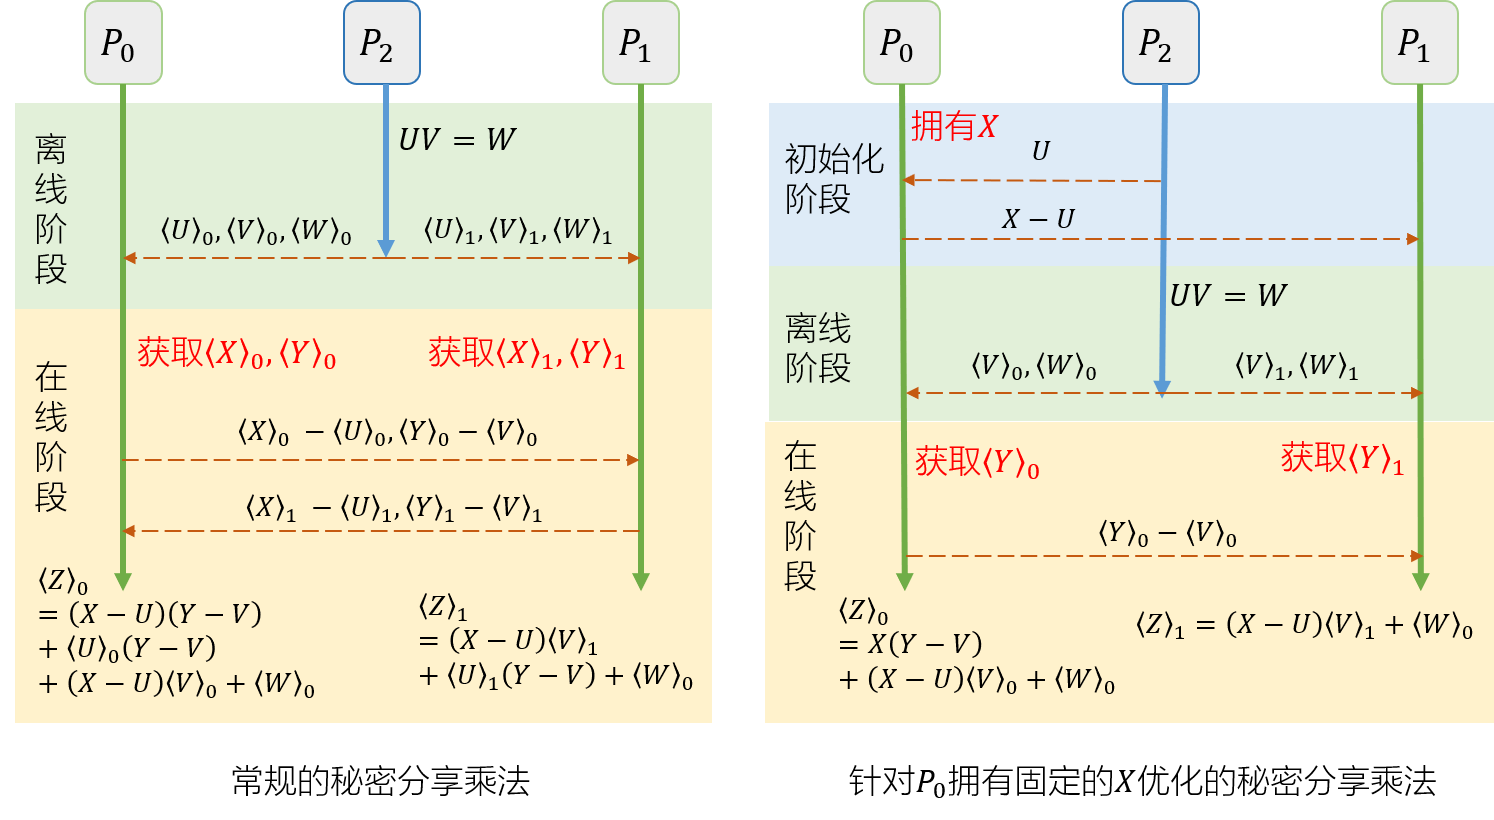
\includegraphics[width=\linewidth]{Z_Resources/perm-llm_ssmul.png}    
    \caption{优化的秘密分享乘法与原始秘密分享乘法的对比}
    \label{fig:perm-llm:ssmul}
\end{figure}


\subsubsection{针对注意力的秘密分享乘法}
在计算注意力分数时,我们需要将当前的查询向量 $\bvec q_i$ 与多个键向量 $\bvec k_1, \cdots, k_n$ 求内积,且注意到在单次文本生成任务中,每轮都会有一个新的键向量加入。
%
如果把键向量构成的矩阵当作$X$,我们可以发现情况与线性层有所类似。
乘数$X$虽然不是固定的,但是其每一轮只会加入一个新的向量,而其余部分保持不变。
%
因此,我们可以借用针对线性层优化的安全秘密分享乘法中的思想,在每一轮在线阶段的运算中,只考虑 $X$ 新增加的部分(此处记作$X'$)恢复出 $X' - U'$,从而更新原有的 $X - U$上。
%
    \chapter{总结与展望}
\section{本文工作总结}
本文深入研究了隐私保护机器学习中的效率和安全问题,针对拆分学习以及密码学和其他方法的混合方法两个方面,对隐私保护机器学习的效率和安全进行了优化,提出了一系列创新性的算法和框架。
%
这些方法在理论上有一定的创新性,同时也有较强的应用价值,可以直接部署在实际的隐私保护机器学习代码框架中。
%

在拆分学习方面,本文的研究围绕着拆分层的表征分布,创新地提出了表征的随机Top-$k$压缩方法和基于势能损失的扰动方法,分别提高了拆分学习的效率和隐私。
%
针对拆分学习的效率问题,本文探究了各种压缩方法应用于拆分学习的拆分层表征的情形,并且从表征分布空间的角度说明了Top-$k$算法在理论上有更强的泛化性能。
进一步地,我们提出随机Top-$k$算法,解决了传统的Top-$k$算法存在的收敛性问题,同时更好地发挥了理论上的泛化性优势,实现了通信高效的拆分学习训练和推理。
此外,压缩拆分层表征也能保护输入特征的隐私。
%
该方法适用于类别数量庞大、拆分层表征维度大的拆分学习模型。
%
针对拆分学习的安全问题,本文探究了拆分层表征分布和攻击效果的关系,提出将模型补全攻击视作一个有监督/无监督学习问题,将攻击效果和泛化误差联系起来。
基于此分析,本文提出了受物理学启发的势能损失函数,对拆分层表征的分布进行扰动,降低了模型补全攻击的效果,显著优于现有的降低距离相关性的方法。
该方法使得拆分层的选取可以更靠近模型输出,从而也间接地保护输入特征的隐私。

在密码学方法和其他方法的结合方面,本文首先针对密码学方法中非线性激活函数计算开销大、拟合存在误差的问题,创新性地提出了使用随机排列方法将非线性激活函数交给半可信第三方计算的方法,从而极大降低了隐私保护神经网络的计算开销。
此外,本文详细研究了随机排列和直接暴露中间结果的隐私泄露量化方法,采用距离相关性指标对隐私泄露进行了量化分析,证明了随机排列具有很强的隐私保护性能。
在此基础上,本文将随机排列方法推广至大语言模型,根据大语言模型推断过程的特性进行了优化,提高了秘密分享乘法效率;并且采用安全排列协议,将基于排列的非线性函数计算协议的在线计算由三方减少为两方,提高了安全性和通用性;此外,使用基于同态加密的隐匿查询手段来解码最终的预测单词。
%
该方法将大语言模型的隐私推断的开销降低到秒级别,效率相比于已有的密码学方法有超过百倍的提升。


\section{未来工作展望}
针对本文上述的研究工作,在隐私保护机器学习的效率和安全方面,有以下几个问题可以在未来深入研究:
%

针对拆分学习的通信压缩问题,进一步将稀疏化和量化结合起来提高通信效率,并且可以调研根据拆分层的具体结构针对性地进行压缩:如拆分层为卷积层时,更多地使用量化方法避免丢失过多信息;拆分层为全连接层时,则考虑将量化和稀疏化结合。
将通信压缩与神经网络架构搜索(Neural Architecture Search)~\cite{renpengzhen_2021_nas_survey}结合,自动化地根据具体场景找到最优压缩方案。
此外,通信压缩对拆分学习安全性的影响也值得深入研究。

针对拆分学习的安全问题,需要进一步对隐层表征的数据分布对于攻击者泛化误差的影响进行深入研究,需要考虑多分类情形,探究更加精确的量化关系。
探究新的扰动方法,如变分推断~\cite{kingma_2014_vae,alemi_2022_deep_variational}等应用于拆分学习隐层表征的效果。
研究拆分学习训练场景中的隐私保护,特别是对梯度中包含的标签信息的保护。

针对密码学和随机排列的混合方法,可以进一步对随机排列的安全性进行研究,并且结合多精度训练等方法进一步提高隐私保护神经网络的效率。
%
探究线下阶段的半可信第三方的安全性增强,如通过区块链~\cite{belotti_2019_blockchain}等技术将单一的半可信第三方转化为多个隐私服务提供方,通过共识机制(Consensus Mechanism)等方案共同保证安全性,实现更加实用的隐私保护机器学习框架。
%
探究全同态加密(Fully Homomorphic Encryption)技术与秘密分享、随机排列的结合,特别是优化线性计算部分,减少秘密分享带来的高通信量性能瓶颈,也是未来值得研究的方向。
}



% \chapter{关于本模板}

% 本模板根据浙江大学研究生院编写的《浙江大学研究生学位论文编写规则》~\cite{zjugradthesisrules},
% 在原有的 zjuthesis 模板~\cite{zjuthesis}基础上开发而来。

% 本模板的本科生版本\cite{zjuthesisrules}得到了浙江大学本科生院老师的支持与审核,
% 已经在本科生院网上公示。
% 但当前的研究生版本并未经过研究生院老师的审核,
% 同学们使用时要注意对照模板与要求,
% 切不可盲目使用。

% 作者本人并未编写过浙江大学研究生毕业论文,
% 所以不清楚具体要求。
% 如果有热心同学愿意帮忙,
% 可以替我联系相关老师,我会配合审核并修改代码。

% \section{Overleaf 使用注意事项}

% 如果你在Overleaf上编译本模板,请注意如下事项:

% \begin{itemize}
%     \item 删除根目录的 ``.latexmkrc'' 文件,否则编译失败且不报任何错误
%     \item 字体有版权所以本模板不能附带字体,请务必手动上传字体文件,并在各个专业模板下手动指定字体。
%         具体方法参照 GitHub 主页的说明。
%     \item 当前的Overleaf默认使用TexLive 2017进行编译,但一些伪粗体复制乱码的问题需要TexLive 2019版本来解决。
%         所以各位同学可以在Overleaf上编写论文时务必切换到TexLive 2019或更新版本来编译,以免产生查重相关问题。
%         具体说明参照 GitHub 主页。
% \end{itemize}


% \section{节标题}

% 我们可以用includegraphics来插入现有的jpg等格式的图片,
% 如\autoref{fig:zju-logo}所示。

% \begin{figure}[htbp]
%     \centering
%     
\includegraphics[width=.3\linewidth]{logo/zju}
%     \caption{\label{fig:zju-logo}浙江大学LOGO}
% \end{figure}


% \subsection{小节标题}


% \par 如\autoref{tab:sample}所示,这是一张自动调节列宽的表格。

% \begin{table}[htbp]
%     \caption{\label{tab:sample}自动调节列宽的表格}
%     \begin{tabularx}{\linewidth}{c|X<{\centering}}
%         \hline
%         第一列 & 第二列 \\ \hline
%         xxx & xxx \\ \hline
%         xxx & xxx \\ \hline
%         xxx & xxx \\ \hline
%     \end{tabularx}
% \end{table}


% \par 如\autoref{equ:sample},这是一个公式

% \begin{equation}
%     \label{equ:sample}
%     A=\overbrace{(a+b+c)+\underbrace{i(d+e+f)}_{\text{虚数}}}^{\text{复数}}
% \end{equation}

% \chapter{另一章}


% \begin{figure}[htbp]
%     \centering
%     \includegraphics[width=.3\linewidth]{example-image-a}
%     \caption{\label{fig:fig-placeholder}图片占位符}
% \end{figure}

% \chapter{再一章}

% \par 如\autoref{alg:sample},这是一个算法

% % \begin{algorithm}[H]
% %     \begin{algorithmic} % enter the algorithmic environment
% %         \REQUIRE $n \geq 0 \vee x \neq 0$
% %         \ENSURE $y = x^n$
% %         \STATE $y \Leftarrow 1$
% %         \IF{$n < 0$}
% %             \STATE $X \Leftarrow 1 / x$
% %             \STATE $N \Leftarrow -n$
% %         \ELSE
% %             \STATE $X \Leftarrow x$
% %             \STATE $N \Leftarrow n$
% %         \ENDIF
% %         \WHILE{$N \neq 0$}
% %             \IF{$N$ is even}
% %                 \STATE $X \Leftarrow X \times X$
% %                 \STATE $N \Leftarrow N / 2$
% %             \ELSE[$N$ is odd]
% %                 \STATE $y \Leftarrow y \times X$
% %                 \STATE $N \Leftarrow N - 1$
% %             \ENDIF
% %         \ENDWHILE
% %     \end{algorithmic}
% %     \caption{\label{alg:sample}算法样例}
% % \end{algorithm}